\documentclass[twoside]{book}

% Packages required by doxygen
\usepackage{fixltx2e}
\usepackage{calc}
\usepackage{doxygen}
\usepackage[export]{adjustbox} % also loads graphicx
\usepackage{graphicx}
\usepackage[utf8]{inputenc}
\usepackage{makeidx}
\usepackage{multicol}
\usepackage{multirow}
\PassOptionsToPackage{warn}{textcomp}
\usepackage{textcomp}
\usepackage[nointegrals]{wasysym}
\usepackage[table]{xcolor}

% Font selection
\usepackage[T1]{fontenc}
\usepackage[scaled=.90]{helvet}
\usepackage{courier}
\usepackage{amssymb}
\usepackage{sectsty}
\renewcommand{\familydefault}{\sfdefault}
\allsectionsfont{%
  \fontseries{bc}\selectfont%
  \color{darkgray}%
}
\renewcommand{\DoxyLabelFont}{%
  \fontseries{bc}\selectfont%
  \color{darkgray}%
}
\newcommand{\+}{\discretionary{\mbox{\scriptsize$\hookleftarrow$}}{}{}}

% Page & text layout
\usepackage{geometry}
\geometry{%
  a4paper,%
  top=2.5cm,%
  bottom=2.5cm,%
  left=2.5cm,%
  right=2.5cm%
}
\tolerance=750
\hfuzz=15pt
\hbadness=750
\setlength{\emergencystretch}{15pt}
\setlength{\parindent}{0cm}
\setlength{\parskip}{0.2cm}
\makeatletter
\renewcommand{\paragraph}{%
  \@startsection{paragraph}{4}{0ex}{-1.0ex}{1.0ex}{%
    \normalfont\normalsize\bfseries\SS@parafont%
  }%
}
\renewcommand{\subparagraph}{%
  \@startsection{subparagraph}{5}{0ex}{-1.0ex}{1.0ex}{%
    \normalfont\normalsize\bfseries\SS@subparafont%
  }%
}
\makeatother

% Headers & footers
\usepackage{fancyhdr}
\pagestyle{fancyplain}
\fancyhead[LE]{\fancyplain{}{\bfseries\thepage}}
\fancyhead[CE]{\fancyplain{}{}}
\fancyhead[RE]{\fancyplain{}{\bfseries\leftmark}}
\fancyhead[LO]{\fancyplain{}{\bfseries\rightmark}}
\fancyhead[CO]{\fancyplain{}{}}
\fancyhead[RO]{\fancyplain{}{\bfseries\thepage}}
\fancyfoot[LE]{\fancyplain{}{}}
\fancyfoot[CE]{\fancyplain{}{}}
\fancyfoot[RE]{\fancyplain{}{\bfseries\scriptsize Generated on Sat Dec 12 2015 22\+:20\+:39 for Graybat by Doxygen }}
\fancyfoot[LO]{\fancyplain{}{\bfseries\scriptsize Generated on Sat Dec 12 2015 22\+:20\+:39 for Graybat by Doxygen }}
\fancyfoot[CO]{\fancyplain{}{}}
\fancyfoot[RO]{\fancyplain{}{}}
\renewcommand{\footrulewidth}{0.4pt}
\renewcommand{\chaptermark}[1]{%
  \markboth{#1}{}%
}
\renewcommand{\sectionmark}[1]{%
  \markright{\thesection\ #1}%
}

% Indices & bibliography
\usepackage{natbib}
\usepackage[titles]{tocloft}
\setcounter{tocdepth}{3}
\setcounter{secnumdepth}{5}
\makeindex

% Hyperlinks (required, but should be loaded last)
\usepackage{ifpdf}
\ifpdf
  \usepackage[pdftex,pagebackref=true]{hyperref}
\else
  \usepackage[ps2pdf,pagebackref=true]{hyperref}
\fi
\hypersetup{%
  colorlinks=true,%
  linkcolor=blue,%
  citecolor=blue,%
  unicode%
}

% Custom commands
\newcommand{\clearemptydoublepage}{%
  \newpage{\pagestyle{empty}\cleardoublepage}%
}


%===== C O N T E N T S =====

\begin{document}

% Titlepage & ToC
\hypersetup{pageanchor=false,
             bookmarks=true,
             bookmarksnumbered=true,
             pdfencoding=unicode
            }
\pagenumbering{roman}
\begin{titlepage}
\vspace*{7cm}
\begin{center}%
{\Large Graybat \\[1ex]\large 1.\+0 }\\
\vspace*{1cm}
{\large Generated by Doxygen 1.8.10}\\
\vspace*{0.5cm}
{\small Sat Dec 12 2015 22:20:39}\\
\end{center}
\end{titlepage}
\clearemptydoublepage
\tableofcontents
\clearemptydoublepage
\pagenumbering{arabic}
\hypersetup{pageanchor=true}

%--- Begin generated contents ---
\chapter{Gray\+Bat}
\label{index}\hypertarget{index}{}{\bfseries Gr}aph {\bfseries A}pproach for Highl{\bfseries y} Generic Communication Schemes {\bfseries B}ased on {\bfseries A}daptive {\bfseries T}opologies

\subsection*{Description}

{\bfseries Gray\+Bat} is a C++ library that presents a graph-\/based communication approach, which enables a mapping of algorithms to communication patterns and further a mapping of these communication patterns to varying hardware architectures. Therefore, a flexible and configurable communication approach for parallel and distributed applications. These mappings are established as an intermediate layer between an application and communication libraries and are dynamically adptable during run-\/time.

An application supported by Gray\+Bat can be created with the following steps\+:


\begin{DoxyEnumerate}
\item Decide on how fine grain the application domain should be decomposed
\item Model communication pattern of subdomains as a graph
\item Choose mapping of graph vertices to peers
\item Choose hardware to run the application on
\end{DoxyEnumerate}



The \hyperlink{cage}{communication and graph environment} (cage) is the central class of Gray\+Bat. The cage provides both communication and graph operations to enable communication based on graphs and is a good point to {\bfseries get started}. Otherwise consider the \hyperlink{gol}{Game of Life} example simulation which provides a full demonstration of utilizing Gray\+Bat.

\subsection*{Further Links}


\begin{DoxyItemize}
\item \hyperlink{cage}{Communication and Graph Environment}
\item \hyperlink{tutorial}{Graybat Tutorials} 
\end{DoxyItemize}
\chapter{Communication and Graph Environment}
\label{cage}
\hypertarget{cage}{}
The communication and graph environment (\hyperlink{structgraybat_1_1Cage}{cage}) provides a graph-\/based virtual overlay network which is implemented by the policy based design. Taking this term to pieces, the \hyperlink{structgraybat_1_1Cage}{cage} is an interface which provides communication methods on basis of an existing communication library, where the possible paths of communication are described by a graph.

The behavior of the \hyperlink{structgraybat_1_1Cage}{cage} need to be defined by a \hyperlink{communicationPolicy}{communication policy} and a \hyperlink{graphPolicy}{graph policy}. These policies need to be provided as template arguments to the \hyperlink{structgraybat_1_1Cage}{cage} class. The following listings show examples on how to use and how to configure the \hyperlink{structgraybat_1_1Cage}{cage} with predefined \hyperlink{communicationPolicy}{communication policy} and \hyperlink{graphPolicy}{graph policy}.

\subsection*{Configure the graybat cage}


\begin{DoxyEnumerate}
\item Include graybat cage, communication policy, graph policy and predefined functors for communication patterns and mappings. 
\begin{DoxyCode}
\textcolor{preprocessor}{#include <graybat/Cage.hpp>}
\textcolor{preprocessor}{#include <graybat/communicationPolicy/BMPI.hpp>}
\textcolor{preprocessor}{#include <graybat/graphPolicy/BGL.hpp>}
\textcolor{preprocessor}{#include <graybat/pattern/GridDiagonal.hpp>}
\textcolor{preprocessor}{#include <graybat/mapping/Consecutive.hpp>}
\end{DoxyCode}

\item Define communication policy to use (boost.\+M\+P\+I). 
\begin{DoxyCode}
\textcolor{keyword}{typedef} \hyperlink{structgraybat_1_1communicationPolicy_1_1BMPI}{graybat::communicationPolicy::BMPI}   CommunicationPolicy;
\textcolor{keyword}{typedef} \textcolor{keyword}{typename} CommunicationPolicy::Config Config;
\end{DoxyCode}

\item Define graph policy to use (boost graph library). 
\begin{DoxyCode}
\textcolor{keyword}{typedef} \hyperlink{classgraybat_1_1graphPolicy_1_1BGL}{graybat::graphPolicy::BGL<>} GraphPolicy;
\end{DoxyCode}

\item Define cage through policies. 
\begin{DoxyCode}
\textcolor{keyword}{typedef} \hyperlink{structgraybat_1_1Cage}{graybat::Cage<CommunicatonPolicy, GraphPolicy>} Cage;
\end{DoxyCode}

\item Create Cage instance and set graph creation functor that describes the communication \hyperlink{communicationPattern}{pattern}. 
\begin{DoxyCode}
Cage cage;
cage.setGraph(\hyperlink{structgraybat_1_1pattern_1_1GridDiagonal}{graybat::pattern::GridDiagonal}(100,100))
\end{DoxyCode}

\end{DoxyEnumerate}

\subsection*{Mapping Operations}


\begin{DoxyEnumerate}
\item {\bfseries distribute}\+: Distributes vertices of the graph to peer(s) based on a \hyperlink{mapping}{mapping}. 
\begin{DoxyCode}
cage.distribute(\hyperlink{structgraybat_1_1mapping_1_1Consecutive}{graybat::mapping::Consecutive}());
\end{DoxyCode}

\item {\bfseries hosted\+Vertices}\+: The vertices mapped to the peer itself are called hosted vertices. 
\begin{DoxyCode}
\textcolor{keyword}{typedef} Cage::Vertex Vertex;

\textcolor{comment}{// Iterate over all vertices that I host}
\textcolor{keywordflow}{for}(Vertex vertex: cage.hostedVertices)\{
    std::cout << vertex.id << std::endl;
\}
\end{DoxyCode}

\end{DoxyEnumerate}

\subsection*{Graph Operations}

A peer is responsible for the communication of all its hosted vertices. Therefore, the common approach for communication in graybat is to iterate over the set of hosted vertices and send data to adjacent vertices which are connected with an outgoing edge and receive data from adjacent vertices which are connected with an incoming edge.


\begin{DoxyEnumerate}
\item {\bfseries get\+Out\+Edges}\+: Retrieve outgoing edges of hosted vertices. This information can be used to send data to adjacent vertices. 
\begin{DoxyCode}
\textcolor{keyword}{typedef} Cage::Edge Edge;
\textcolor{keywordflow}{for}(Vertex vertex: cage.hostedVertices)\{
    \textcolor{keywordflow}{for}(Edge outEdge : cage.getOutEdges(vertex))\{
        Vertex sourceVertex = outEdge.source;
        Vertex targetVertex = outEdge.target;

        std::cout << \textcolor{stringliteral}{"From vertex "} << sourceVertex.id
                  << \textcolor{stringliteral}{"over edge "}   << outEdge.id
                  << \textcolor{stringliteral}{"to vertex "}   << targetVertex.id << std::endl;
    \}
\}
\end{DoxyCode}

\item {\bfseries get\+In\+Edges}\+: Retrieve incoming edges of hosted vertices. This information can be used to receive data from adjacent vertices. 
\begin{DoxyCode}
\textcolor{keywordflow}{for}(Vertex vertex: cage.hostedVertices)\{
    \textcolor{keywordflow}{for}(Edge inEdge : cage.getInEdges(vertex))\{
        Vertex sourceVertex = inEdge.source;
        Vertex targetVertex = inEdge.target;

        std::cout << \textcolor{stringliteral}{"From vertex "} << sourceVertex.id
                  << \textcolor{stringliteral}{"over edge "}   << inEdge.id
                  << \textcolor{stringliteral}{"to vertex "}   << targetVertex.id << std::endl;
    \}
\}
\end{DoxyCode}

\end{DoxyEnumerate}

\subsection*{Point to Point Communication Operations}


\begin{DoxyItemize}
\item {\bfseries send/async\+Send}\+: Send synchronous and asynchronous data. The asynchronous version of send returns an event, which can be waited for or tested for its state. 
\begin{DoxyCode}
\textcolor{keyword}{typedef} Cage::Edge  Edge;
\textcolor{keyword}{typedef} Cage::Event Event;

\textcolor{comment}{// Events that will occur}
std::vector<Event> events;

\textcolor{comment}{// Some data that should be send}
std::vector<int> data(100,1);

\textcolor{keywordflow}{for}(Vertex vertex: cage.hostedVertices)\{
    \textcolor{keywordflow}{for}(Edge outEdge : cage.getOutEdges(vertex))\{

          \textcolor{comment}{// Synchronous}
      cage.send(outEdge, data);

      \textcolor{comment}{// Asynchronous}
      cage.send(outEdge, data, events);

          \textcolor{comment}{// Wait for and test event}
      events.back().wait();
      \textcolor{keywordtype}{bool} eventState = events.back().ready();
    \}
\}
\end{DoxyCode}

\item {\bfseries recv/async\+Recv}\+: Receive synchronous and asynchronous data. The asynchronous version of recv returns an event, which can be waited for or tested for its state. 
\begin{DoxyCode}
\textcolor{keyword}{typedef} Cage::Edge  Edge;
\textcolor{keyword}{typedef} Cage::Event Event;

\textcolor{comment}{// Events that will occur}
std::vector<Event> events;

\textcolor{comment}{// Some data that should be send}
std::vector<int> data(100,1);

\textcolor{keywordflow}{for}(Vertex vertex: cage.hostedVertices)\{
    \textcolor{keywordflow}{for}(Edge inEdge : cage.getInEdges(vertex))\{

        \textcolor{comment}{// Synchronous receive}
        cage.recv(inEdge, data);

        \textcolor{comment}{// Asynchronous receive}
        cage.recv(inEdge, data, events);

        \textcolor{comment}{// Wait for and test event}
        events.back().wait();
        \textcolor{keywordtype}{bool} eventState = events.back().ready();
    \}
\}
\end{DoxyCode}

\end{DoxyItemize}

\subsection*{Collective Communication Operations}


\begin{DoxyItemize}
\item {\bfseries spread}\+: Spread data to all adjacent vertices of a vertex that are connected by an outgoing edge. 
\begin{DoxyCode}
\textcolor{keyword}{typedef} Cage::Edge  Edge;
\textcolor{keyword}{typedef} Cage::Event Event;

\textcolor{comment}{// Events that will occur}
std::vector<Event> events;

\textcolor{comment}{// Some data that should be send}
std::vector<int> data(100,1);

\textcolor{keywordflow}{for}(Vertex vertex: cage.hostedVertices)\{
    cage.spread(vertex, data, events);
\}
\end{DoxyCode}

\item {\bfseries collect}\+: Collect data from all adjacent vertices of a vertex that are connected by an incoming edge. 
\begin{DoxyCode}
\textcolor{keyword}{typedef} Cage::Edge  Edge;
\textcolor{keyword}{typedef} Cage::Event Event;

\textcolor{comment}{// Events that will occur}
std::vector<Event> events;

\textcolor{keywordflow}{for}(Vertex vertex: cage.hostedVertices)\{
    \textcolor{comment}{// Some data that should be collected}
    std::vector<int> data(vertex.nInEdges * 100, 1);

    cage.collect(vertex, data);
\}
\end{DoxyCode}

\item {\bfseries reduce}\+: Reduce vector of data with binary operator and receive by some root vertex. 
\begin{DoxyCode}
Vertex rootVertex = cage.getVertex(0);

std::vector<int> send(100);
std::vector<int> recv(100);

\textcolor{comment}{// Each vertex need to reduce its data, the root receives reduction.}
\textcolor{keywordflow}{for}(Vertex vertex: cage.hostedVertices)\{
    cage.reduce(rootVertex, vertex, std::plus<int>, send, recv);
\}
\end{DoxyCode}

\item {\bfseries all\+Reduce}\+: Reduce vector of data and receive them by every vertex. 
\begin{DoxyCode}
std::vector<int> send(100);
std::vector<int> recv(100);

\textcolor{comment}{// Each vertex need to reduce its data, all receive reduction.}
\textcolor{keywordflow}{for}(Vertex vertex: cage.hostedVertices)\{
    cage.allReduce(rootVertex, vertex, std::plus<int>, send, recv);
\}
\end{DoxyCode}

\item {\bfseries gather}\+: Root vertex collects data from each vertex. 
\begin{DoxyCode}
Vertex rootVertex = cage.getVertex(0);

std::vector<int> send(10);
std::vector<int> recv(10 * cage.getVertices().size());

\textcolor{comment}{// Each vertex need to send its data, the root receives}
\textcolor{keywordflow}{for}(Vertex vertex: cage.hostedVertices)\{
    cage.gather(rootVertex, vertex, send, recv);
\}
\end{DoxyCode}

\item {\bfseries all\+Gather}\+: Data is send to all vertices. 
\begin{DoxyCode}
std::vector<int> send(10);
std::vector<int> recv(10 * cage.getVertices().size());

\textcolor{comment}{// Each vertex need to send its data, all receive.}
\textcolor{keywordflow}{for}(Vertex vertex: cage.hostedVertices)\{
    cage.allGather(vertex, send, recv);
\}
\end{DoxyCode}

\item {\bfseries synchronize}\+: Synchronize all peers (including their hosted vertices). 
\begin{DoxyCode}
cage.synchronize();
\end{DoxyCode}

\end{DoxyItemize}

\subsection*{Further Links}


\begin{DoxyItemize}
\item \hyperlink{communicationPolicy}{Communication Policy}
\item \hyperlink{graphPolicy}{Graph Policy}
\item \hyperlink{communicationPattern}{Communication Pattern}
\item \hyperlink{mapping}{Vertex Mapping}
\item \hyperlink{vertex}{Vertex Communication Interface}
\item \hyperlink{edge}{Edge Communication Interface} 
\end{DoxyItemize}\hypertarget{communicationPolicy}{}\section{Communication Policy}\label{communicationPolicy}
The communication policy is a class which implements the communication interface of its host class (\hyperlink{cage}{cage}).

Communication in graybat is modeled in the way, that an instance that takes part on whatever communication is called a {\itshape peer}. All peers that want to communicate in some way with each other need to group up in a \hyperlink{context}{context}. Therefore, a \hyperlink{context}{context} is a set of peers that are able to communicate with each other.

By communication is meant the exchange of arbitrary data between peers or even within one peer. Thus, communication can mean sending a message over the internet, copying data between two memories, or distributing data with the help of M\+P\+I. Therefore, a communication policy need to implement the required interface but can interpret the term communication on its own. See the code example below or consider the preimplemented communication policies.

The communication policy interface is separated into core and collective api. The core api provides the \hyperlink{context}{context} type definition, the \hyperlink{event}{event} type definition, {\bfseries point-\/to-\/point communication} methods and {\bfseries context management} methods, while the collective api contains {\bfseries collective communication} methods. The communication policy needs to implement at least the core api, the collective api based on the core api can be derived from the communication policy {\bfseries \hyperlink{structgraybat_1_1communicationPolicy_1_1Base}{graybat\+::communication\+Policy\+::\+Base}} class. Thus, it is possible to provide a communication policy implementation that does not implement all interface (core + collective) methods.

The following source code provides a basic skeleton of a communication policy\+:


\begin{DoxyCode}
\textcolor{keyword}{namespace }\hyperlink{namespacegraybat}{graybat} \{

    \textcolor{keyword}{namespace }communicationPolicy \{

        \textcolor{keyword}{namespace }traits \{

            \textcolor{keyword}{template}<>
            \textcolor{keyword}{struct }ContextType<CommunicationPolicySkeleton> \{
                \textcolor{keyword}{using} type = ...;
            \};

            \textcolor{keyword}{template}<>
            \textcolor{keyword}{struct }EventType<CommunicationPolicySkeleton> \{
                \textcolor{keyword}{using} type = ...;
            \};

            \textcolor{keyword}{template}<>
            \textcolor{keyword}{struct }ConfigType<CommunicationPolicySkeleton> \{
                \textcolor{keyword}{using} type = ...;
            \};

        \}

        \textcolor{keyword}{struct }CommunicationPolicySkeleton : \textcolor{keyword}{public} 
      \hyperlink{structgraybat_1_1communicationPolicy_1_1Base}{graybat::communicationPolicy::Base}<CommunicationPolicySkeleton> \{


            \textcolor{comment}{/*******************************************************************}
\textcolor{comment}{               COMMUNICATION POLICY CONSTRUCTIOn}
\textcolor{comment}{             ******************************************************************/}
            ZMQ(Config \textcolor{keyword}{const} config) \{...\}


            \textcolor{comment}{/*******************************************************************}
\textcolor{comment}{               POINT TO POINT COMMUNICATION INTERFACE}
\textcolor{comment}{             ******************************************************************/}
            \textcolor{keywordtype}{void} send(\textcolor{keyword}{const} VAddr destVAddr, \textcolor{keyword}{const} \hyperlink{structTag}{Tag} tag, \textcolor{keyword}{const} Context context, \textcolor{keyword}{const} T\_Send& 
      sendData) \{...\}

            Event asyncSend(\textcolor{keyword}{const} VAddr destVAddr, \textcolor{keyword}{const} \hyperlink{structTag}{Tag} tag, \textcolor{keyword}{const} Context context, T\_Send& 
      sendData) \{...\}

            \textcolor{keywordtype}{void} recv(\textcolor{keyword}{const} VAddr srcVAddr, \textcolor{keyword}{const} \hyperlink{structTag}{Tag} tag, \textcolor{keyword}{const} Context context, T\_Recv& recvData) \{...
      \}

            Event recv(\textcolor{keyword}{const} Context context, T\_Recv& recvData) \{...\}


            \textcolor{comment}{/*******************************************************************}
\textcolor{comment}{               CONTEXT MANAGEMENT INTERFACE}
\textcolor{comment}{             ******************************************************************/}
            Context splitContext(\textcolor{keyword}{const} \textcolor{keywordtype}{bool} isMember, \textcolor{keyword}{const} Context oldContext) \{...\}

            Context getGlobalContext()\{...\}

        \};

    \} \textcolor{comment}{/* namespace communicationPolicy*/}

\} \textcolor{comment}{/* namespace graybat */}
\end{DoxyCode}


\subsection*{Further Links}


\begin{DoxyItemize}
\item \hyperlink{structgraybat_1_1communicationPolicy_1_1BMPI}{graybat\+::communication\+Policy\+::\+B\+M\+P\+I}
\item \hyperlink{structgraybat_1_1communicationPolicy_1_1ZMQ}{graybat\+::communication\+Policy\+::\+Z\+M\+Q}
\item \hyperlink{context}{Context}
\item \hyperlink{event}{Event} 
\end{DoxyItemize}\hypertarget{context}{}\subsection{Context}\label{context}
A context is a set of peers which are able to communicate with each other. A context need to be defined by a \hyperlink{communicationPolicy}{communication policy}, since every communication library defines a set of peers differently. The \hyperlink{cage}{cage} defines a strict interface of a context, but the implementation is left open to the \hyperlink{communicationPolicy}{communication policy}.

The following listing provides a skeleton for a context class with all necessary methods\+:


\begin{DoxyCode}
struc ContextSkeleton \{

    \textcolor{comment}{// Returns the number of peers in this context}
    \textcolor{keywordtype}{size\_t} size()\textcolor{keyword}{ const }\{...\}

    \textcolor{comment}{// Returns the virtual address of the peer in this context}
    VAddr getVAddr()\textcolor{keyword}{ const }\{...\}

    \textcolor{comment}{// Returns the id of this context}
    ContextID getID()\textcolor{keyword}{ const }\{...\}

    \textcolor{comment}{// Returns whether the peer is member of the context}
    \textcolor{keywordtype}{bool} valid()\textcolor{keyword}{ const }\{...\}

\};
\end{DoxyCode}
 \hypertarget{event}{}\subsection{Event}\label{event}
An event is a class that is returned by non-\/blocking or asynchronous communication functions like graybat\+::\+Cage\+::async\+Send or graybat\+::\+Cage\+::async\+Recv. Each \hyperlink{communicationPolicy}{communication policy} needs to define its event class, since this can be very library dependent. The \hyperlink{cage}{cage} determines a strict event interface, but leaves their implementation open to the \hyperlink{communicationPolicy}{communication policy}.

The following listing provides a skeleton for a event class with all necessary methods\+:


\begin{DoxyCode}
\textcolor{keyword}{struct }EventSkeleton \{

    \textcolor{comment}{// Wait for the event to be finished}
    \textcolor{keywordtype}{void} wait() \{...\}

    \textcolor{comment}{// Ask for current state of the event}
    \textcolor{keywordtype}{bool} ready() \{...\}

        \textcolor{comment}{// Ask for VAddr where message of event comes from}
        VAddr source() \{...\}

        \textcolor{comment}{// Ask for the tag the message of this event was send with}
        \hyperlink{structTag}{Tag} getTag() \{...\}
\};
\end{DoxyCode}
 \hypertarget{graphPolicy}{}\section{Graph Policy}\label{graphPolicy}
The graph policy is a class which implements the graph interface of its host class (\hyperlink{cage}{cage}). A graph is defined by its vertex and edge property through template arguments and its graph description as constructor argument. The following defintion of a graph is defined by a city property which represents a vertex and a road property which represents an edge\+:


\begin{DoxyCode}
\textcolor{keyword}{typedef} \hyperlink{classgraybat_1_1graphPolicy_1_1BGL}{graybat::graphPolicy::BGL<City, Road>} CityGraph;
\end{DoxyCode}


The following property is a very simple and basic property for edges and vertices which does not contain any further information. Therefore, it is called Simple\+Property. The Simple\+Property is used when no other property is specified.


\begin{DoxyCode}
\textcolor{keyword}{struct }SimpleProperty \{

\};
\end{DoxyCode}


A property can be user defined and can contain arbitrary data\+:


\begin{DoxyCode}
\textcolor{keyword}{struct }City \{
    std::string cityName;
    \textcolor{keywordtype}{unsigned} nInhabitants;
\};

\textcolor{keyword}{struct }Road \{
    std::string roadName;
\};
\end{DoxyCode}


The following source code provides the full skeleton of a graph policy. Nevertheless, the predefined boost graph library graph policy (\hyperlink{classgraybat_1_1graphPolicy_1_1BGL}{graybat\+::graph\+Policy\+::\+B\+G\+L}) is a good starting point to be used in a \hyperlink{cage}{cage}. A custom implementation might only be necessary if there exist some special requirements.


\begin{DoxyCode}
\textcolor{keyword}{namespace }\hyperlink{namespacegraybat}{graybat} \{

        \textcolor{keyword}{namespace }graphPolicy \{

                \textcolor{keyword}{template} <\textcolor{keyword}{class} T\_VertexProperty, \textcolor{keyword}{class} T\_EdgeProperty>
                \textcolor{keyword}{class }GraphPolicySkeleton \{

                        \textcolor{comment}{/*******************************************************************}
\textcolor{comment}{                           REQUIRED TYPE DEFINITIONS}
\textcolor{comment}{                         ******************************************************************/}
                        \textcolor{keyword}{using} VertexProperty     = T\_VertexProperty;
                        \textcolor{keyword}{using} EdgeProperty       = T\_EdgeProperty;
                        \textcolor{keyword}{using} VertexDescription  = ...;
                        \textcolor{keyword}{using} EdgeDescription    = ...;
                        \textcolor{keyword}{using} GraphDescription   = ...;
                        \textcolor{keyword}{using} InEdgeIter         = ...;
                        \textcolor{keyword}{using} OutEdgeIter        = ...;
                        \textcolor{keyword}{using} AdjacentVertexIter = ...;
                        \textcolor{keyword}{using} AllVertexIter      = ...;

                        \textcolor{comment}{/*******************************************************************}
\textcolor{comment}{                           GRAPH CONSTRUCTION}
\textcolor{comment}{                         ******************************************************************/}
                        GraphPolicySkeleton(GraphDescription description) \{...\}

                        \textcolor{comment}{/*******************************************************************}
\textcolor{comment}{                           REQUIRED GRAPH OPERATIONS}
\textcolor{comment}{                         ******************************************************************/}

                        std::pair<AllVertexIter, AllVertexIter> getVertices() \{...\}

                        std::pair<EdgeID, bool> getEdge(\textcolor{keyword}{const} VertexID source, \textcolor{keyword}{const} VertexID target) \{...\}
       

                        std::pair<AdjacentVertexIter, AdjacentVertexIter> getAdjacentVertices(\textcolor{keyword}{const} 
      VertexID \textcolor{keywordtype}{id}) \{...\}

                        std::pair<OutEdgeIter, OutEdgeIter> getOutEdges(\textcolor{keyword}{const} VertexID \textcolor{keywordtype}{id}) \{...\}

                        std::pair<InEdgeIter, InEdgeIter> getInEdges(\textcolor{keyword}{const} VertexID \textcolor{keywordtype}{id})\{...\}

                        std::pair<VertexID, VertexProperty>& getVertexProperty(\textcolor{keyword}{const} VertexID vertex) \{...\}

                        std::pair<EdgeID, EdgeProperty>& getEdgeProperty(\textcolor{keyword}{const} EdgeID edge) \{...\}

                        VertexID getEdgeTarget(\textcolor{keyword}{const} EdgeID edge) \{...\}

                        VertexID getEdgeSource(\textcolor{keyword}{const} EdgeID edge) \{...\}

                \}
        \}
\}
\end{DoxyCode}


\subsection*{Further Links}


\begin{DoxyItemize}
\item \hyperlink{classgraybat_1_1graphPolicy_1_1BGL}{graybat\+::graph\+Policy\+::\+B\+G\+L} 
\end{DoxyItemize}\hypertarget{communicationPattern}{}\section{Communication Pattern}\label{communicationPattern}
A communication pattern is a class functor which generates a graph. They are used to define the communication graph of a \hyperlink{cage}{cage}. Gray\+Bat provides a handful of predefined pattern\+:


\begin{DoxyItemize}
\item \hyperlink{structgraybat_1_1pattern_1_1FullyConnected}{graybat\+::pattern\+::\+Fully\+Connected}
\item \hyperlink{structgraybat_1_1pattern_1_1GridDiagonal}{graybat\+::pattern\+::\+Grid\+Diagonal}
\item \hyperlink{structgraybat_1_1pattern_1_1Grid}{graybat\+::pattern\+::\+Grid}
\item \hyperlink{structgraybat_1_1pattern_1_1HyperCube}{graybat\+::pattern\+::\+Hyper\+Cube}
\item \hyperlink{structgraybat_1_1pattern_1_1InStar}{graybat\+::pattern\+::\+In\+Star}
\item \hyperlink{structgraybat_1_1pattern_1_1OutStar}{graybat\+::pattern\+::\+Out\+Star}
\item \hyperlink{structgraybat_1_1pattern_1_1BiStar}{graybat\+::pattern\+::\+Bi\+Star}
\item \hyperlink{structgraybat_1_1pattern_1_1EdgeLess}{graybat\+::pattern\+::\+Edge\+Less}
\item \hyperlink{structgraybat_1_1pattern_1_1Ring}{graybat\+::pattern\+::\+Ring}
\item \hyperlink{structgraybat_1_1pattern_1_1None}{graybat\+::pattern\+::\+None}
\end{DoxyItemize}

Own communication pattern can be build from the following pattern skeleton\+: 
\begin{DoxyCode}
\textcolor{keyword}{namespace }\hyperlink{namespacegraybat}{graybat} \{

  \textcolor{keyword}{namespace }pattern \{

    \textcolor{keyword}{struct }PatternSkeleton \{

        \textcolor{comment}{// Functor which returns a desired graph}
        GraphDescription operator()()\{
    \};

  \} \textcolor{comment}{/* pattern */}

\} \textcolor{comment}{/* graybat */}
\end{DoxyCode}


\subsection*{Further Links}


\begin{DoxyItemize}
\item \hyperlink{structgraybat_1_1pattern_1_1FullyConnected}{graybat\+::pattern\+::\+Fully\+Connected}
\item \hyperlink{structgraybat_1_1pattern_1_1GridDiagonal}{graybat\+::pattern\+::\+Grid\+Diagonal}
\item \hyperlink{structgraybat_1_1pattern_1_1Grid}{graybat\+::pattern\+::\+Grid}
\item \hyperlink{structgraybat_1_1pattern_1_1HyperCube}{graybat\+::pattern\+::\+Hyper\+Cube}
\item \hyperlink{structgraybat_1_1pattern_1_1InStar}{graybat\+::pattern\+::\+In\+Star}
\item \hyperlink{structgraybat_1_1pattern_1_1OutStar}{graybat\+::pattern\+::\+Out\+Star}
\item \hyperlink{structgraybat_1_1pattern_1_1BiStar}{graybat\+::pattern\+::\+Bi\+Star}
\item \hyperlink{structgraybat_1_1pattern_1_1EdgeLess}{graybat\+::pattern\+::\+Edge\+Less}
\item \hyperlink{structgraybat_1_1pattern_1_1Ring}{graybat\+::pattern\+::\+Ring}
\item \hyperlink{structgraybat_1_1pattern_1_1None}{graybat\+::pattern\+::\+None} 
\end{DoxyItemize}\hypertarget{mapping}{}\section{Vertex Mapping}\label{mapping}
A vertex mapping is a class functor which describes the mapping of a graph to peers. A mapping is used by the \hyperlink{cage}{cage} in its \hyperlink{structgraybat_1_1Cage_afeddcc035e25382462c38c77b481304d}{graybat\+::\+Cage\+::distribute} function and can strongly influence the application performance.\+Gray\+Bat defines a handful of predefined mappings\+:


\begin{DoxyItemize}
\item \hyperlink{structgraybat_1_1mapping_1_1Consecutive}{graybat\+::mapping\+::\+Consecutive}
\item \hyperlink{structgraybat_1_1mapping_1_1Filter}{graybat\+::mapping\+::\+Filter}
\item \hyperlink{structgraybat_1_1mapping_1_1GraphPartition}{graybat\+::mapping\+::\+Graph\+Partition}
\item \hyperlink{structgraybat_1_1mapping_1_1Random}{graybat\+::mapping\+::\+Random}
\item \hyperlink{structgraybat_1_1mapping_1_1Roundrobin}{graybat\+::mapping\+::\+Roundrobin}
\end{DoxyItemize}

Own vertex mappings can be build from the following mapping skeleton\+:


\begin{DoxyCode}
\textcolor{keyword}{namespace }\hyperlink{namespacegraybat}{graybat} \{

    \textcolor{keyword}{namespace }mapping \{

        \textcolor{keyword}{struct }MappingSkeleton \{

            \textcolor{keyword}{template}<\textcolor{keyword}{typename} T\_Cage>
            std::vector<typename T\_Graph::Vertex> operator()(\textcolor{keyword}{const} \textcolor{keywordtype}{unsigned} processID, \textcolor{keyword}{const} \textcolor{keywordtype}{unsigned} 
      processCount, T\_Cage &cage) \{...\}

        \};

    \} \textcolor{comment}{/* mapping */}

\} \textcolor{comment}{/* graybat */}
\end{DoxyCode}


\subsection*{Further Links}


\begin{DoxyItemize}
\item \hyperlink{structgraybat_1_1mapping_1_1Consecutive}{graybat\+::mapping\+::\+Consecutive}
\item \hyperlink{structgraybat_1_1mapping_1_1Filter}{graybat\+::mapping\+::\+Filter}
\item \hyperlink{structgraybat_1_1mapping_1_1GraphPartition}{graybat\+::mapping\+::\+Graph\+Partition}
\item \hyperlink{structgraybat_1_1mapping_1_1Random}{graybat\+::mapping\+::\+Random}
\item \hyperlink{structgraybat_1_1mapping_1_1Roundrobin}{graybat\+::mapping\+::\+Roundrobin} 
\end{DoxyItemize}\hypertarget{vertex}{}\section{Vertex Communication Interface}\label{vertex}
Next to the communication methods provided by the \hyperlink{cage}{cage} a vertex also provides methods to communicate with its adjacent vertices.

It is assume that a \hyperlink{cage}{cage} has allready been instantiated and initialised.


\begin{DoxyEnumerate}
\item Collect data from all incoming edges\+: 
\begin{DoxyCode}
\textcolor{comment}{// Just get a vertex from the cage}
Vertex vertex = cage.getVertex(0);

\textcolor{comment}{// Prepare the receive container}
std::vector<T\_Data> collectData(vertex.nInEdges());

\textcolor{comment}{// Synchronous recv messages from all incoming edges}
vertex.collect(recvData);
\end{DoxyCode}
 This functionality is also available in the cage\+: 
\begin{DoxyCode}
cage.collect(vertex, collectData);
\end{DoxyCode}

\item Spread data to all outgoing edges\+: 
\begin{DoxyCode}
\textcolor{comment}{// Again, take some random vertex}
Vertex vertex = cage.getVertex(0);

\textcolor{comment}{// Prepare the container to spread}
std::vector<T\_Data> spreadData(1, static\_cast<T\_Data>(1));

\textcolor{comment}{// Synchron send same data over all outgoing edges}
v.spread(spreadData);

\textcolor{comment}{// Asynchron send same data over all outgoing edges}
std::vector<Event> events;
v.spread(sendData, events);
\end{DoxyCode}

\end{DoxyEnumerate}

\subsection*{Further Links}


\begin{DoxyItemize}
\item \hyperlink{structgraybat_1_1CommunicationVertex}{graybat\+::\+Communication\+Vertex} 
\end{DoxyItemize}\hypertarget{edge}{}\section{Edge Communication Interface}\label{edge}
Next to the communication methods provided by the \hyperlink{cage}{cage} a edge also provides methods to communicate with its connected vertex

It is assume that a \hyperlink{cage}{cage} has allready been instantiated and initialised.


\begin{DoxyCode}
\textcolor{comment}{// Just get a vertex from the cage}
Edge edge = cage.getVertex(0).getOutEdges()[0]

\textcolor{comment}{// Prepare send container}
std::vector<T\_Data> sendData(10);

\textcolor{comment}{// Send data over edge}
edge << sendData;

\textcolor{comment}{// Recv data over inverse edge}
edge.inverse() >> recvData
\end{DoxyCode}


\subsection*{Further Links}


\begin{DoxyItemize}
\item \hyperlink{structgraybat_1_1CommunicationEdge}{graybat\+::\+Communication\+Edge} 
\end{DoxyItemize}
\chapter{Graybat Tutorials}
\label{tutorial}
\hypertarget{tutorial}{}

\begin{DoxyItemize}
\item \hyperlink{zmq}{Run Zero\+M\+Q Communication Policy}
\item \hyperlink{gol}{The Game of Life Example} 
\end{DoxyItemize}\hypertarget{zmq}{}\section{Run Zero\+M\+Q Communication Policy}\label{zmq}
The Zero\+M\+Q communication policy needs a connection to the zmq signaling server. The connection parameters need to be provided through the Zero\+M\+Q specific communication policy configuration. This configuration contains\+:


\begin{DoxyItemize}
\item Url of the signaling server
\item Own Url
\item Context size
\end{DoxyItemize}


\begin{DoxyCode}
\textcolor{keywordtype}{int} main()\{

    \textcolor{keyword}{using} GP         = \hyperlink{classgraybat_1_1graphPolicy_1_1BGL}{graybat::graphPolicy::BGL<>};
    \textcolor{keyword}{using} ZMQ        = \hyperlink{structgraybat_1_1communicationPolicy_1_1ZMQ}{graybat::communicationPolicy::ZMQ};
    \textcolor{keyword}{using} ZMQCage    = \hyperlink{structgraybat_1_1Cage}{graybat::Cage<ZMQ, GP>};
    \textcolor{keyword}{using} ZMQConfig  = \hyperlink{structgraybat_1_1communicationPolicy_1_1zmq_1_1Config}{graybat::communicationPolicy::zmq::Config};

    ZMQConfig zmqConfig = \{\textcolor{stringliteral}{"tcp://127.0.0.1:5000"},
                           \textcolor{stringliteral}{"tcp://127.0.0.1:5001"},
                           \textcolor{keyword}{static\_cast<}\textcolor{keywordtype}{size\_t}\textcolor{keyword}{>}(std::stoi(std::getenv(\textcolor{stringliteral}{"OMPI\_COMM\_WORLD\_SIZE"})))\};

    ZMQCage zmqCage(zmqConfig);

\}
\end{DoxyCode}


First the signaling server needs to be started.


\begin{DoxyCode}
$ ./zmq\_signaling --ip 127:0.0.1 --port 5000 &
\end{DoxyCode}


Afterwards, an application using the Zero\+M\+Q communication policy can be started by {\ttfamily mpiexec}.


\begin{DoxyCode}
$ mpiexec -n 4 ./a.out
\end{DoxyCode}


\subsection*{Further Links}


\begin{DoxyItemize}
\item \hyperlink{structgraybat_1_1communicationPolicy_1_1ZMQ}{graybat\+::communication\+Policy\+::\+Z\+M\+Q}
\item \hyperlink{structgraybat_1_1communicationPolicy_1_1zmq_1_1Config}{graybat\+::communication\+Policy\+::zmq\+::\+Config} 
\end{DoxyItemize}\hypertarget{gol}{}\section{The Game of Life Example}\label{gol}
The following figure shows a sketch of the game of life simulation implemented with Gray\+Bat support. The Game of Life domain (20 x 20 cells) is decomposed very fine grain, such that, every cell is represented by a vertex in a two-\/dimensional grid and neighboring vertices are connected by edges (\hyperlink{structgraybat_1_1pattern_1_1GridDiagonal}{graybat\+::pattern\+::\+Grid\+Diagonal}). The graph is partioned into four partitions and mapped to four peers (graybat\+::pattern\+::\+Graph\+Partition). Therefore, each peer is responsible for the communication of 100 vertices with its neighbors. Finally, each two peers are mapped to a quad core processor on a dual socket system (\hyperlink{structgraybat_1_1communicationPolicy_1_1BMPI}{graybat\+::communication\+Policy\+::\+B\+M\+P\+I}). This is one possible sequence of mappings for a Game of Life simulation within the Gray\+Bat framework. On each step changes are possible to adapt the simulation to other architectures, networks or algorithms.



\subsection*{See Also}


\begin{DoxyItemize}
\item \hyperlink{gol_8cpp-example}{Go\+L Sources}
\item \hyperlink{cage}{Communication and Graph Environment}
\item \hyperlink{communicationPolicy}{Communication Policy}
\item \hyperlink{graphPolicy}{Graph Policy}
\item \hyperlink{communicationPattern}{Communication Pattern}
\item \hyperlink{mapping}{Vertex Mapping} 
\end{DoxyItemize}
\chapter{Hierarchical Index}
\section{Class Hierarchy}
This inheritance list is sorted roughly, but not completely, alphabetically\+:\begin{DoxyCompactList}
\item \contentsline{section}{graybat\+:\+:communication\+Policy\+:\+:Base$<$ T\+\_\+\+Communication\+Policy $>$}{\pageref{structgraybat_1_1communicationPolicy_1_1Base}}{}
\item \contentsline{section}{graybat\+:\+:communication\+Policy\+:\+:Base$<$ B\+M\+P\+I $>$}{\pageref{structgraybat_1_1communicationPolicy_1_1Base}}{}
\begin{DoxyCompactList}
\item \contentsline{section}{graybat\+:\+:communication\+Policy\+:\+:B\+M\+P\+I}{\pageref{structgraybat_1_1communicationPolicy_1_1BMPI}}{}
\end{DoxyCompactList}
\item \contentsline{section}{graybat\+:\+:communication\+Policy\+:\+:Base$<$ Z\+M\+Q $>$}{\pageref{structgraybat_1_1communicationPolicy_1_1Base}}{}
\begin{DoxyCompactList}
\item \contentsline{section}{graybat\+:\+:communication\+Policy\+:\+:Z\+M\+Q}{\pageref{structgraybat_1_1communicationPolicy_1_1ZMQ}}{}
\end{DoxyCompactList}
\item \contentsline{section}{graybat\+:\+:graph\+Policy\+:\+:B\+G\+L$<$ T\+\_\+\+Vertex\+Property, T\+\_\+\+Edge\+Property $>$}{\pageref{classgraybat_1_1graphPolicy_1_1BGL}}{}
\item \contentsline{section}{graybat\+:\+:graph\+Policy\+:\+:B\+G\+L$<$ Vertex\+Property, Edge\+Property $>$}{\pageref{classgraybat_1_1graphPolicy_1_1BGL}}{}
\item \contentsline{section}{graybat\+:\+:pattern\+:\+:Bi\+Star$<$ T\+\_\+\+Graph\+Policy $>$}{\pageref{structgraybat_1_1pattern_1_1BiStar}}{}
\item \contentsline{section}{graybat\+:\+:Cage$<$ T\+\_\+\+Communication\+Policy, T\+\_\+\+Graph\+Policy $>$}{\pageref{structgraybat_1_1Cage}}{}
\item \contentsline{section}{Cell}{\pageref{structCell}}{}
\item \contentsline{section}{graybat\+:\+:pattern\+:\+:Chain$<$ T\+\_\+\+Graph\+Policy $>$}{\pageref{structgraybat_1_1pattern_1_1Chain}}{}
\item \contentsline{section}{graybat\+:\+:Communication\+Edge$<$ T\+\_\+\+Cage $>$}{\pageref{structgraybat_1_1CommunicationEdge}}{}
\item \contentsline{section}{graybat\+:\+:Communication\+Vertex$<$ T\+\_\+\+Cage $>$}{\pageref{structgraybat_1_1CommunicationVertex}}{}
\item \contentsline{section}{graybat\+:\+:communication\+Policy\+:\+:zmq\+:\+:Config}{\pageref{structgraybat_1_1communicationPolicy_1_1zmq_1_1Config}}{}
\item \contentsline{section}{graybat\+:\+:communication\+Policy\+:\+:bmpi\+:\+:Config}{\pageref{structgraybat_1_1communicationPolicy_1_1bmpi_1_1Config}}{}
\item \contentsline{section}{graybat\+:\+:communication\+Policy\+:\+:traits\+:\+:Config\+Type$<$ T\+\_\+\+Communication\+Policy $>$}{\pageref{structgraybat_1_1communicationPolicy_1_1traits_1_1ConfigType}}{}
\item \contentsline{section}{graybat\+:\+:communication\+Policy\+:\+:traits\+:\+:Config\+Type$<$ B\+M\+P\+I $>$}{\pageref{structgraybat_1_1communicationPolicy_1_1traits_1_1ConfigType_3_01BMPI_01_4}}{}
\item \contentsline{section}{graybat\+:\+:communication\+Policy\+:\+:traits\+:\+:Config\+Type$<$ Z\+M\+Q $>$}{\pageref{structgraybat_1_1communicationPolicy_1_1traits_1_1ConfigType_3_01ZMQ_01_4}}{}
\item \contentsline{section}{graybat\+:\+:mapping\+:\+:Consecutive}{\pageref{structgraybat_1_1mapping_1_1Consecutive}}{}
\item \contentsline{section}{graybat\+:\+:communication\+Policy\+:\+:Min\+B\+M\+P\+I\+:\+:Context}{\pageref{classgraybat_1_1communicationPolicy_1_1MinBMPI_1_1Context}}{}
\item \contentsline{section}{graybat\+:\+:communication\+Policy\+:\+:bmpi\+:\+:Context}{\pageref{classgraybat_1_1communicationPolicy_1_1bmpi_1_1Context}}{}
\item \contentsline{section}{graybat\+:\+:communication\+Policy\+:\+:zmq\+:\+:Context$<$ T\+\_\+\+C\+P $>$}{\pageref{classgraybat_1_1communicationPolicy_1_1zmq_1_1Context}}{}
\item \contentsline{section}{graybat\+:\+:communication\+Policy\+:\+:traits\+:\+:Context\+Type$<$ T\+\_\+\+Communication\+Policy $>$}{\pageref{structgraybat_1_1communicationPolicy_1_1traits_1_1ContextType}}{}
\item \contentsline{section}{graybat\+:\+:communication\+Policy\+:\+:traits\+:\+:Context\+Type$<$ B\+M\+P\+I $>$}{\pageref{structgraybat_1_1communicationPolicy_1_1traits_1_1ContextType_3_01BMPI_01_4}}{}
\item \contentsline{section}{graybat\+:\+:communication\+Policy\+:\+:traits\+:\+:Context\+Type$<$ Z\+M\+Q $>$}{\pageref{structgraybat_1_1communicationPolicy_1_1traits_1_1ContextType_3_01ZMQ_01_4}}{}
\item \contentsline{section}{graybat\+:\+:pattern\+:\+:Edge\+Less$<$ T\+\_\+\+Graph\+Policy $>$}{\pageref{structgraybat_1_1pattern_1_1EdgeLess}}{}
\item \contentsline{section}{graybat\+:\+:communication\+Policy\+:\+:Min\+B\+M\+P\+I\+:\+:Event}{\pageref{classgraybat_1_1communicationPolicy_1_1MinBMPI_1_1Event}}{}
\item \contentsline{section}{graybat\+:\+:communication\+Policy\+:\+:zmq\+:\+:Event$<$ T\+\_\+\+C\+P $>$}{\pageref{classgraybat_1_1communicationPolicy_1_1zmq_1_1Event}}{}
\item \contentsline{section}{graybat\+:\+:communication\+Policy\+:\+:bmpi\+:\+:Event}{\pageref{classgraybat_1_1communicationPolicy_1_1bmpi_1_1Event}}{}
\item \contentsline{section}{graybat\+:\+:communication\+Policy\+:\+:traits\+:\+:Event\+Type$<$ T\+\_\+\+Communication\+Policy $>$}{\pageref{structgraybat_1_1communicationPolicy_1_1traits_1_1EventType}}{}
\item \contentsline{section}{graybat\+:\+:communication\+Policy\+:\+:traits\+:\+:Event\+Type$<$ B\+M\+P\+I $>$}{\pageref{structgraybat_1_1communicationPolicy_1_1traits_1_1EventType_3_01BMPI_01_4}}{}
\item \contentsline{section}{graybat\+:\+:communication\+Policy\+:\+:traits\+:\+:Event\+Type$<$ Z\+M\+Q $>$}{\pageref{structgraybat_1_1communicationPolicy_1_1traits_1_1EventType_3_01ZMQ_01_4}}{}
\item \contentsline{section}{graybat\+:\+:mapping\+:\+:Filter}{\pageref{structgraybat_1_1mapping_1_1Filter}}{}
\item \contentsline{section}{graybat\+:\+:pattern\+:\+:Fully\+Connected$<$ T\+\_\+\+Graph\+Policy $>$}{\pageref{structgraybat_1_1pattern_1_1FullyConnected}}{}
\item \contentsline{section}{Function}{\pageref{structFunction}}{}
\item \contentsline{section}{graybat\+:\+:mapping\+:\+:Graph\+Partition}{\pageref{structgraybat_1_1mapping_1_1GraphPartition}}{}
\item \contentsline{section}{graybat\+:\+:pattern\+:\+:Grid$<$ T\+\_\+\+Graph\+Policy $>$}{\pageref{structgraybat_1_1pattern_1_1Grid}}{}
\item \contentsline{section}{graybat\+:\+:pattern\+:\+:Grid\+Diagonal$<$ T\+\_\+\+Graph\+Policy $>$}{\pageref{structgraybat_1_1pattern_1_1GridDiagonal}}{}
\item \contentsline{section}{graybat\+:\+:pattern\+:\+:Hyper\+Cube$<$ T\+\_\+\+Graph\+Policy $>$}{\pageref{structgraybat_1_1pattern_1_1HyperCube}}{}
\item \contentsline{section}{graybat\+:\+:pattern\+:\+:In\+Star$<$ T\+\_\+\+Graph\+Policy $>$}{\pageref{structgraybat_1_1pattern_1_1InStar}}{}
\item \contentsline{section}{graybat\+:\+:Cage$<$ T\+\_\+\+Communication\+Policy, T\+\_\+\+Graph\+Policy $>$\+:\+:maximum$<$ T $>$}{\pageref{structgraybat_1_1Cage_1_1maximum}}{}
\item \contentsline{section}{graybat\+:\+:communication\+Policy\+:\+:Min\+B\+M\+P\+I}{\pageref{structgraybat_1_1communicationPolicy_1_1MinBMPI}}{}
\item \contentsline{section}{graybat\+:\+:pattern\+:\+:None$<$ T\+\_\+\+Graph\+Policy $>$}{\pageref{structgraybat_1_1pattern_1_1None}}{}
\item \contentsline{section}{graybat\+:\+:pattern\+:\+:Out\+Star$<$ T\+\_\+\+Graph\+Policy $>$}{\pageref{structgraybat_1_1pattern_1_1OutStar}}{}
\item \contentsline{section}{graybat\+:\+:mapping\+:\+:Random}{\pageref{structgraybat_1_1mapping_1_1Random}}{}
\item \contentsline{section}{graybat\+:\+:pattern\+:\+:Ring$<$ T\+\_\+\+Graph\+Policy $>$}{\pageref{structgraybat_1_1pattern_1_1Ring}}{}
\item \contentsline{section}{graybat\+:\+:mapping\+:\+:Roundrobin}{\pageref{structgraybat_1_1mapping_1_1Roundrobin}}{}
\item \contentsline{section}{graybat\+:\+:graph\+Policy\+:\+:Simple\+Property}{\pageref{structgraybat_1_1graphPolicy_1_1SimpleProperty}}{}
\item \contentsline{section}{Tag}{\pageref{structTag}}{}
\end{DoxyCompactList}

\chapter{Class Index}
\section{Class List}
Here are the classes, structs, unions and interfaces with brief descriptions\+:\begin{DoxyCompactList}
\item\contentsline{section}{\hyperlink{structgraybat_1_1communicationPolicy_1_1Base}{graybat\+::communication\+Policy\+::\+Base$<$ T\+\_\+\+Communication\+Policy $>$} }{\pageref{structgraybat_1_1communicationPolicy_1_1Base}}{}
\item\contentsline{section}{\hyperlink{classgraybat_1_1graphPolicy_1_1BGL}{graybat\+::graph\+Policy\+::\+B\+G\+L$<$ T\+\_\+\+Vertex\+Property, T\+\_\+\+Edge\+Property $>$} \\*A class to describe directed graphs }{\pageref{classgraybat_1_1graphPolicy_1_1BGL}}{}
\item\contentsline{section}{\hyperlink{structgraybat_1_1pattern_1_1BiStar}{graybat\+::pattern\+::\+Bi\+Star$<$ T\+\_\+\+Graph\+Policy $>$} }{\pageref{structgraybat_1_1pattern_1_1BiStar}}{}
\item\contentsline{section}{\hyperlink{structgraybat_1_1communicationPolicy_1_1BMPI}{graybat\+::communication\+Policy\+::\+B\+M\+P\+I} \\*Implementation of the \hyperlink{structgraybat_1_1Cage}{Cage} communication\+Policy interface based on the M\+P\+I implementation boost\+::mpi }{\pageref{structgraybat_1_1communicationPolicy_1_1BMPI}}{}
\item\contentsline{section}{\hyperlink{structgraybat_1_1Cage}{graybat\+::\+Cage$<$ T\+\_\+\+Communication\+Policy, T\+\_\+\+Graph\+Policy $>$} \\*The Communication And Graph Environment enables to communicate on basis of a graph with methods of a user defined communication library }{\pageref{structgraybat_1_1Cage}}{}
\item\contentsline{section}{\hyperlink{structCell}{Cell} }{\pageref{structCell}}{}
\item\contentsline{section}{\hyperlink{structgraybat_1_1pattern_1_1Chain}{graybat\+::pattern\+::\+Chain$<$ T\+\_\+\+Graph\+Policy $>$} }{\pageref{structgraybat_1_1pattern_1_1Chain}}{}
\item\contentsline{section}{\hyperlink{structgraybat_1_1CommunicationEdge}{graybat\+::\+Communication\+Edge$<$ T\+\_\+\+Cage $>$} }{\pageref{structgraybat_1_1CommunicationEdge}}{}
\item\contentsline{section}{\hyperlink{structgraybat_1_1CommunicationVertex}{graybat\+::\+Communication\+Vertex$<$ T\+\_\+\+Cage $>$} }{\pageref{structgraybat_1_1CommunicationVertex}}{}
\item\contentsline{section}{\hyperlink{structgraybat_1_1communicationPolicy_1_1zmq_1_1Config}{graybat\+::communication\+Policy\+::zmq\+::\+Config} }{\pageref{structgraybat_1_1communicationPolicy_1_1zmq_1_1Config}}{}
\item\contentsline{section}{\hyperlink{structgraybat_1_1communicationPolicy_1_1bmpi_1_1Config}{graybat\+::communication\+Policy\+::bmpi\+::\+Config} }{\pageref{structgraybat_1_1communicationPolicy_1_1bmpi_1_1Config}}{}
\item\contentsline{section}{\hyperlink{structgraybat_1_1communicationPolicy_1_1traits_1_1ConfigType}{graybat\+::communication\+Policy\+::traits\+::\+Config\+Type$<$ T\+\_\+\+Communication\+Policy $>$} }{\pageref{structgraybat_1_1communicationPolicy_1_1traits_1_1ConfigType}}{}
\item\contentsline{section}{\hyperlink{structgraybat_1_1communicationPolicy_1_1traits_1_1ConfigType_3_01BMPI_01_4}{graybat\+::communication\+Policy\+::traits\+::\+Config\+Type$<$ B\+M\+P\+I $>$} }{\pageref{structgraybat_1_1communicationPolicy_1_1traits_1_1ConfigType_3_01BMPI_01_4}}{}
\item\contentsline{section}{\hyperlink{structgraybat_1_1communicationPolicy_1_1traits_1_1ConfigType_3_01ZMQ_01_4}{graybat\+::communication\+Policy\+::traits\+::\+Config\+Type$<$ Z\+M\+Q $>$} }{\pageref{structgraybat_1_1communicationPolicy_1_1traits_1_1ConfigType_3_01ZMQ_01_4}}{}
\item\contentsline{section}{\hyperlink{structgraybat_1_1mapping_1_1Consecutive}{graybat\+::mapping\+::\+Consecutive} }{\pageref{structgraybat_1_1mapping_1_1Consecutive}}{}
\item\contentsline{section}{\hyperlink{classgraybat_1_1communicationPolicy_1_1MinBMPI_1_1Context}{graybat\+::communication\+Policy\+::\+Min\+B\+M\+P\+I\+::\+Context} \\*A context represents a set of peers which are able to communicate with each other }{\pageref{classgraybat_1_1communicationPolicy_1_1MinBMPI_1_1Context}}{}
\item\contentsline{section}{\hyperlink{classgraybat_1_1communicationPolicy_1_1bmpi_1_1Context}{graybat\+::communication\+Policy\+::bmpi\+::\+Context} }{\pageref{classgraybat_1_1communicationPolicy_1_1bmpi_1_1Context}}{}
\item\contentsline{section}{\hyperlink{classgraybat_1_1communicationPolicy_1_1zmq_1_1Context}{graybat\+::communication\+Policy\+::zmq\+::\+Context$<$ T\+\_\+\+C\+P $>$} \\*A context represents a set of peers which are able to communicate with each other }{\pageref{classgraybat_1_1communicationPolicy_1_1zmq_1_1Context}}{}
\item\contentsline{section}{\hyperlink{structgraybat_1_1communicationPolicy_1_1traits_1_1ContextType}{graybat\+::communication\+Policy\+::traits\+::\+Context\+Type$<$ T\+\_\+\+Communication\+Policy $>$} }{\pageref{structgraybat_1_1communicationPolicy_1_1traits_1_1ContextType}}{}
\item\contentsline{section}{\hyperlink{structgraybat_1_1communicationPolicy_1_1traits_1_1ContextType_3_01BMPI_01_4}{graybat\+::communication\+Policy\+::traits\+::\+Context\+Type$<$ B\+M\+P\+I $>$} }{\pageref{structgraybat_1_1communicationPolicy_1_1traits_1_1ContextType_3_01BMPI_01_4}}{}
\item\contentsline{section}{\hyperlink{structgraybat_1_1communicationPolicy_1_1traits_1_1ContextType_3_01ZMQ_01_4}{graybat\+::communication\+Policy\+::traits\+::\+Context\+Type$<$ Z\+M\+Q $>$} }{\pageref{structgraybat_1_1communicationPolicy_1_1traits_1_1ContextType_3_01ZMQ_01_4}}{}
\item\contentsline{section}{\hyperlink{structgraybat_1_1pattern_1_1EdgeLess}{graybat\+::pattern\+::\+Edge\+Less$<$ T\+\_\+\+Graph\+Policy $>$} }{\pageref{structgraybat_1_1pattern_1_1EdgeLess}}{}
\item\contentsline{section}{\hyperlink{classgraybat_1_1communicationPolicy_1_1MinBMPI_1_1Event}{graybat\+::communication\+Policy\+::\+Min\+B\+M\+P\+I\+::\+Event} \\*An event is returned by non-\/blocking communication operations and can be asked whether an operation has finished or it can be waited for this operation to be finished }{\pageref{classgraybat_1_1communicationPolicy_1_1MinBMPI_1_1Event}}{}
\item\contentsline{section}{\hyperlink{classgraybat_1_1communicationPolicy_1_1zmq_1_1Event}{graybat\+::communication\+Policy\+::zmq\+::\+Event$<$ T\+\_\+\+C\+P $>$} \\*An event is returned by non-\/blocking communication operations and can be asked whether an operation has finished or it can be waited for this operation to be finished }{\pageref{classgraybat_1_1communicationPolicy_1_1zmq_1_1Event}}{}
\item\contentsline{section}{\hyperlink{classgraybat_1_1communicationPolicy_1_1bmpi_1_1Event}{graybat\+::communication\+Policy\+::bmpi\+::\+Event} \\*An event is returned by non-\/blocking communication operations and can be asked whether an operation has finished or it can be waited for this operation to be finished }{\pageref{classgraybat_1_1communicationPolicy_1_1bmpi_1_1Event}}{}
\item\contentsline{section}{\hyperlink{structgraybat_1_1communicationPolicy_1_1traits_1_1EventType}{graybat\+::communication\+Policy\+::traits\+::\+Event\+Type$<$ T\+\_\+\+Communication\+Policy $>$} }{\pageref{structgraybat_1_1communicationPolicy_1_1traits_1_1EventType}}{}
\item\contentsline{section}{\hyperlink{structgraybat_1_1communicationPolicy_1_1traits_1_1EventType_3_01BMPI_01_4}{graybat\+::communication\+Policy\+::traits\+::\+Event\+Type$<$ B\+M\+P\+I $>$} }{\pageref{structgraybat_1_1communicationPolicy_1_1traits_1_1EventType_3_01BMPI_01_4}}{}
\item\contentsline{section}{\hyperlink{structgraybat_1_1communicationPolicy_1_1traits_1_1EventType_3_01ZMQ_01_4}{graybat\+::communication\+Policy\+::traits\+::\+Event\+Type$<$ Z\+M\+Q $>$} }{\pageref{structgraybat_1_1communicationPolicy_1_1traits_1_1EventType_3_01ZMQ_01_4}}{}
\item\contentsline{section}{\hyperlink{structgraybat_1_1mapping_1_1Filter}{graybat\+::mapping\+::\+Filter} }{\pageref{structgraybat_1_1mapping_1_1Filter}}{}
\item\contentsline{section}{\hyperlink{structgraybat_1_1pattern_1_1FullyConnected}{graybat\+::pattern\+::\+Fully\+Connected$<$ T\+\_\+\+Graph\+Policy $>$} }{\pageref{structgraybat_1_1pattern_1_1FullyConnected}}{}
\item\contentsline{section}{\hyperlink{structFunction}{Function} }{\pageref{structFunction}}{}
\item\contentsline{section}{\hyperlink{structgraybat_1_1mapping_1_1GraphPartition}{graybat\+::mapping\+::\+Graph\+Partition} }{\pageref{structgraybat_1_1mapping_1_1GraphPartition}}{}
\item\contentsline{section}{\hyperlink{structgraybat_1_1pattern_1_1Grid}{graybat\+::pattern\+::\+Grid$<$ T\+\_\+\+Graph\+Policy $>$} }{\pageref{structgraybat_1_1pattern_1_1Grid}}{}
\item\contentsline{section}{\hyperlink{structgraybat_1_1pattern_1_1GridDiagonal}{graybat\+::pattern\+::\+Grid\+Diagonal$<$ T\+\_\+\+Graph\+Policy $>$} }{\pageref{structgraybat_1_1pattern_1_1GridDiagonal}}{}
\item\contentsline{section}{\hyperlink{structgraybat_1_1pattern_1_1HyperCube}{graybat\+::pattern\+::\+Hyper\+Cube$<$ T\+\_\+\+Graph\+Policy $>$} }{\pageref{structgraybat_1_1pattern_1_1HyperCube}}{}
\item\contentsline{section}{\hyperlink{structgraybat_1_1pattern_1_1InStar}{graybat\+::pattern\+::\+In\+Star$<$ T\+\_\+\+Graph\+Policy $>$} }{\pageref{structgraybat_1_1pattern_1_1InStar}}{}
\item\contentsline{section}{\hyperlink{structgraybat_1_1Cage_1_1maximum}{graybat\+::\+Cage$<$ T\+\_\+\+Communication\+Policy, T\+\_\+\+Graph\+Policy $>$\+::maximum$<$ T $>$} }{\pageref{structgraybat_1_1Cage_1_1maximum}}{}
\item\contentsline{section}{\hyperlink{structgraybat_1_1communicationPolicy_1_1MinBMPI}{graybat\+::communication\+Policy\+::\+Min\+B\+M\+P\+I} \\*Implementation of the \hyperlink{structgraybat_1_1Cage}{Cage} communication\+Policy interface based on the M\+P\+I implementation boost\+::mpi }{\pageref{structgraybat_1_1communicationPolicy_1_1MinBMPI}}{}
\item\contentsline{section}{\hyperlink{structgraybat_1_1pattern_1_1None}{graybat\+::pattern\+::\+None$<$ T\+\_\+\+Graph\+Policy $>$} }{\pageref{structgraybat_1_1pattern_1_1None}}{}
\item\contentsline{section}{\hyperlink{structgraybat_1_1pattern_1_1OutStar}{graybat\+::pattern\+::\+Out\+Star$<$ T\+\_\+\+Graph\+Policy $>$} }{\pageref{structgraybat_1_1pattern_1_1OutStar}}{}
\item\contentsline{section}{\hyperlink{structgraybat_1_1mapping_1_1Random}{graybat\+::mapping\+::\+Random} }{\pageref{structgraybat_1_1mapping_1_1Random}}{}
\item\contentsline{section}{\hyperlink{structgraybat_1_1pattern_1_1Ring}{graybat\+::pattern\+::\+Ring$<$ T\+\_\+\+Graph\+Policy $>$} }{\pageref{structgraybat_1_1pattern_1_1Ring}}{}
\item\contentsline{section}{\hyperlink{structgraybat_1_1mapping_1_1Roundrobin}{graybat\+::mapping\+::\+Roundrobin} }{\pageref{structgraybat_1_1mapping_1_1Roundrobin}}{}
\item\contentsline{section}{\hyperlink{structgraybat_1_1graphPolicy_1_1SimpleProperty}{graybat\+::graph\+Policy\+::\+Simple\+Property} }{\pageref{structgraybat_1_1graphPolicy_1_1SimpleProperty}}{}
\item\contentsline{section}{\hyperlink{structTag}{Tag} }{\pageref{structTag}}{}
\item\contentsline{section}{\hyperlink{structgraybat_1_1communicationPolicy_1_1ZMQ}{graybat\+::communication\+Policy\+::\+Z\+M\+Q} \\*Implementation of the \hyperlink{structgraybat_1_1Cage}{Cage} communication\+Policy interface based on \hyperlink{structgraybat_1_1communicationPolicy_1_1ZMQ}{Z\+M\+Q} }{\pageref{structgraybat_1_1communicationPolicy_1_1ZMQ}}{}
\end{DoxyCompactList}

\chapter{Class Documentation}
\hypertarget{structgraybat_1_1communicationPolicy_1_1Base}{}\section{graybat\+:\+:communication\+Policy\+:\+:Base$<$ T\+\_\+\+Communication\+Policy $>$ Struct Template Reference}
\label{structgraybat_1_1communicationPolicy_1_1Base}\index{graybat\+::communication\+Policy\+::\+Base$<$ T\+\_\+\+Communication\+Policy $>$@{graybat\+::communication\+Policy\+::\+Base$<$ T\+\_\+\+Communication\+Policy $>$}}
\subsection*{Public Types}
\begin{DoxyCompactItemize}
\item 
\hypertarget{structgraybat_1_1communicationPolicy_1_1Base_a8809cc88306f4411eff43b185d4a12ba}{}using {\bfseries Communication\+Policy} = T\+\_\+\+Communication\+Policy\label{structgraybat_1_1communicationPolicy_1_1Base_a8809cc88306f4411eff43b185d4a12ba}

\item 
\hypertarget{structgraybat_1_1communicationPolicy_1_1Base_a61555bfaae515788f4832c0f78bc36f4}{}using {\bfseries V\+Addr} = typename graybat\+::communication\+Policy\+::\+V\+Addr$<$ Communication\+Policy $>$\label{structgraybat_1_1communicationPolicy_1_1Base_a61555bfaae515788f4832c0f78bc36f4}

\item 
\hypertarget{structgraybat_1_1communicationPolicy_1_1Base_aced4ab808a9c345a0e698d21736f3a2c}{}using {\bfseries Tag} = typename graybat\+::communication\+Policy\+::\+Tag$<$ Communication\+Policy $>$\label{structgraybat_1_1communicationPolicy_1_1Base_aced4ab808a9c345a0e698d21736f3a2c}

\item 
\hypertarget{structgraybat_1_1communicationPolicy_1_1Base_a12a885bada327fddc91cfe4515af6471}{}using {\bfseries Context} = typename graybat\+::communication\+Policy\+::\+Context$<$ Communication\+Policy $>$\label{structgraybat_1_1communicationPolicy_1_1Base_a12a885bada327fddc91cfe4515af6471}

\item 
\hypertarget{structgraybat_1_1communicationPolicy_1_1Base_a2fc51f670372dfb2d7f8474a5a0f5e89}{}using {\bfseries Event} = typename graybat\+::communication\+Policy\+::\+Event$<$ Communication\+Policy $>$\label{structgraybat_1_1communicationPolicy_1_1Base_a2fc51f670372dfb2d7f8474a5a0f5e89}

\end{DoxyCompactItemize}
\subsection*{Public Member Functions}
\begin{Indent}{\bf Point to Point Communication Interface}\par
\begin{DoxyCompactItemize}
\item 
\hypertarget{structgraybat_1_1communicationPolicy_1_1Base_a7c7b3cd367ec07fa9d12ebbbb89dabb8}{}{\footnotesize template$<$typename T\+\_\+\+Send $>$ }\\void {\bfseries send} (const V\+Addr dest\+V\+Addr, const \hyperlink{structTag}{Tag} tag, const Context context, const T\+\_\+\+Send \&send\+Data)=delete\label{structgraybat_1_1communicationPolicy_1_1Base_a7c7b3cd367ec07fa9d12ebbbb89dabb8}

\item 
\hypertarget{structgraybat_1_1communicationPolicy_1_1Base_a7dfe96d75727357e0bbac4f8dad93a55}{}{\footnotesize template$<$typename T\+\_\+\+Send $>$ }\\Event {\bfseries async\+Send} (const V\+Addr dest\+V\+Addr, const \hyperlink{structTag}{Tag} tag, const Context context, const T\+\_\+\+Send \&send\+Data)=delete\label{structgraybat_1_1communicationPolicy_1_1Base_a7dfe96d75727357e0bbac4f8dad93a55}

\item 
\hypertarget{structgraybat_1_1communicationPolicy_1_1Base_a1785dcc6035447fc3c2b1cd9fee9a4b5}{}{\footnotesize template$<$typename T\+\_\+\+Recv $>$ }\\void {\bfseries recv} (const V\+Addr src\+V\+Addr, const \hyperlink{structTag}{Tag} tag, const Context context, T\+\_\+\+Recv \&recv\+Data)=delete\label{structgraybat_1_1communicationPolicy_1_1Base_a1785dcc6035447fc3c2b1cd9fee9a4b5}

\item 
\hypertarget{structgraybat_1_1communicationPolicy_1_1Base_a2c7e5b0d65bfa0fcfa3377598eb79882}{}{\footnotesize template$<$typename T\+\_\+\+Recv $>$ }\\Event {\bfseries recv} (const Context context, T\+\_\+\+Recv \&recv\+Data)=delete\label{structgraybat_1_1communicationPolicy_1_1Base_a2c7e5b0d65bfa0fcfa3377598eb79882}

\item 
\hypertarget{structgraybat_1_1communicationPolicy_1_1Base_adee3935d47f527c2802d3b88b546b0a2}{}{\footnotesize template$<$typename T\+\_\+\+Recv $>$ }\\Event {\bfseries async\+Recv} (const V\+Addr src\+V\+Addr, const \hyperlink{structTag}{Tag} tag, const Context context, T\+\_\+\+Recv \&recv\+Data)=delete\label{structgraybat_1_1communicationPolicy_1_1Base_adee3935d47f527c2802d3b88b546b0a2}

\end{DoxyCompactItemize}
\end{Indent}
\begin{Indent}{\bf Collective Communication Interface}\par
\begin{DoxyCompactItemize}
\item 
{\footnotesize template$<$typename T\+\_\+\+Send , typename T\+\_\+\+Recv $>$ }\\void \hyperlink{structgraybat_1_1communicationPolicy_1_1Base_a3db000db20b6cb8fd6e63f3d53e82090}{gather} (const V\+Addr root\+V\+Addr, const Context context, const T\+\_\+\+Send \&send\+Data, T\+\_\+\+Recv \&recv\+Data)
\begin{DoxyCompactList}\small\item\em Collects {\itshape send\+Data} from all peers of the {\itshape context} and transmits it as a list to the peer with {\itshape root\+V\+Addr}. Data of all peers has to be from the {\bfseries same} size. \end{DoxyCompactList}\item 
{\footnotesize template$<$typename T\+\_\+\+Send , typename T\+\_\+\+Recv $>$ }\\void \hyperlink{structgraybat_1_1communicationPolicy_1_1Base_a1434994bead59ef38b6eff8346538f0b}{gather\+Var} (const V\+Addr root\+V\+Addr, const Context context, const T\+\_\+\+Send \&send\+Data, T\+\_\+\+Recv \&recv\+Data, std\+::vector$<$ unsigned $>$ \&recv\+Count)
\begin{DoxyCompactList}\small\item\em Collects {\itshape send\+Data} from all members of the {\itshape context} with {\bfseries varying} size and transmits it as a list to peer with {\itshape root\+V\+Addr}. \end{DoxyCompactList}\item 
{\footnotesize template$<$typename T\+\_\+\+Send , typename T\+\_\+\+Recv $>$ }\\void \hyperlink{structgraybat_1_1communicationPolicy_1_1Base_a1b409ea49d7aba2dee0c83e28dda1b65}{all\+Gather} (Context context, const T\+\_\+\+Send \&send\+Data, T\+\_\+\+Recv \&recv\+Data)
\begin{DoxyCompactList}\small\item\em Collects {\itshape send\+Data} from all members of the {\itshape context} and transmits it as a list to every peer in the {\itshape context} \end{DoxyCompactList}\item 
{\footnotesize template$<$typename T\+\_\+\+Send , typename T\+\_\+\+Recv $>$ }\\void \hyperlink{structgraybat_1_1communicationPolicy_1_1Base_a1bad18907fcc45db9d4a119e726061a8}{all\+Gather\+Var} (const Context context, const T\+\_\+\+Send \&send\+Data, T\+\_\+\+Recv \&recv\+Data, std\+::vector$<$ unsigned $>$ \&recv\+Count)
\begin{DoxyCompactList}\small\item\em Collects {\itshape send\+Data} from all peers of the {\itshape context}. Size of {\itshape send\+Data} can vary in size. The data is received by every peer in the {\itshape context}. \end{DoxyCompactList}\item 
{\footnotesize template$<$typename T\+\_\+\+Send , typename T\+\_\+\+Recv $>$ }\\void \hyperlink{structgraybat_1_1communicationPolicy_1_1Base_af1ed07ce5f107f04926d7b7c39c9834e}{scatter} (const V\+Addr root\+V\+Addr, const Context context, const T\+\_\+\+Send \&send\+Data, T\+\_\+\+Recv \&recv\+Data)
\begin{DoxyCompactList}\small\item\em Distributes {\itshape send\+Data} from peer {\itshape root\+V\+Addr} to all peers in {\itshape context}. Every peer will receive different data. \end{DoxyCompactList}\item 
{\footnotesize template$<$typename T\+\_\+\+Send , typename T\+\_\+\+Recv $>$ }\\void \hyperlink{structgraybat_1_1communicationPolicy_1_1Base_ac4aa66d3ed33c810ae48ae762b432b14}{all\+Scatter} (const Context context, const T\+\_\+\+Send \&send\+Data, T\+\_\+\+Recv \&recv\+Data)
\begin{DoxyCompactList}\small\item\em Distributes {\itshape send\+Data} of all peer in the {\itshape context} to all peers in the {\itshape context}. Every peer will receive data from every other peer (also the own data) \end{DoxyCompactList}\item 
{\footnotesize template$<$typename T\+\_\+\+Send , typename T\+\_\+\+Recv , typename T\+\_\+\+Op $>$ }\\void \hyperlink{structgraybat_1_1communicationPolicy_1_1Base_ad3bf74c91931b35b56fbb54ac535bc14}{reduce} (const V\+Addr root\+V\+Addr, const Context context, const T\+\_\+\+Op op, const T\+\_\+\+Send \&send\+Data, T\+\_\+\+Recv \&recv\+Data)
\begin{DoxyCompactList}\small\item\em Performs a reduction with a binary operator {\itshape op} on all {\itshape send\+Data} elements from all peers whithin the {\itshape context}. The result will be received by the peer with {\itshape root\+V\+Addr}. Binary operations like std\+::plus, std\+::minus can be used. But, they can also be defined as binary operator simular to std\+::plus etc. \end{DoxyCompactList}\item 
{\footnotesize template$<$typename T\+\_\+\+Send , typename T\+\_\+\+Recv , typename T\+\_\+\+Op $>$ }\\void \hyperlink{structgraybat_1_1communicationPolicy_1_1Base_ac77038454619b683f006ba149aea2dcb}{all\+Reduce} (const Context context, T\+\_\+\+Op op, const T\+\_\+\+Send \&send\+Data, T\+\_\+\+Recv \&recv\+Data)
\begin{DoxyCompactList}\small\item\em Performs a reduction with a binary operator {\itshape op} on all {\itshape send\+Data} elements from all peers whithin the {\itshape context}. The result will be received by all peers. \end{DoxyCompactList}\item 
{\footnotesize template$<$typename T\+\_\+\+Send\+Recv $>$ }\\void \hyperlink{structgraybat_1_1communicationPolicy_1_1Base_a431ed56b3d5ade805200b565ce98daa0}{broadcast} (const V\+Addr root\+V\+Addr, const Context context, T\+\_\+\+Send\+Recv \&data)
\begin{DoxyCompactList}\small\item\em Send {\itshape send\+Data} from peer {\itshape root\+V\+Addr} to all peers in {\itshape context}. Every peer will receive the same data. \end{DoxyCompactList}\item 
\hypertarget{structgraybat_1_1communicationPolicy_1_1Base_abc4e72365c6ad134ba6e31abd8fa2163}{}void \hyperlink{structgraybat_1_1communicationPolicy_1_1Base_abc4e72365c6ad134ba6e31abd8fa2163}{synchronize} (const Context context)\label{structgraybat_1_1communicationPolicy_1_1Base_abc4e72365c6ad134ba6e31abd8fa2163}

\begin{DoxyCompactList}\small\item\em Synchronizes all peers within {\itshape context} to the same point in the programm execution (barrier). \end{DoxyCompactList}\end{DoxyCompactItemize}
\end{Indent}


\subsection{Member Function Documentation}
\hypertarget{structgraybat_1_1communicationPolicy_1_1Base_a1b409ea49d7aba2dee0c83e28dda1b65}{}\index{graybat\+::communication\+Policy\+::\+Base@{graybat\+::communication\+Policy\+::\+Base}!all\+Gather@{all\+Gather}}
\index{all\+Gather@{all\+Gather}!graybat\+::communication\+Policy\+::\+Base@{graybat\+::communication\+Policy\+::\+Base}}
\subsubsection[{all\+Gather(\+Context context, const T\+\_\+\+Send \&send\+Data, T\+\_\+\+Recv \&recv\+Data)}]{\setlength{\rightskip}{0pt plus 5cm}template$<$typename T\+\_\+\+Communication\+Policy $>$ template$<$typename T\+\_\+\+Send , typename T\+\_\+\+Recv $>$ void {\bf graybat\+::communication\+Policy\+::\+Base}$<$ T\+\_\+\+Communication\+Policy $>$\+::all\+Gather (
\begin{DoxyParamCaption}
\item[{Context}]{context, }
\item[{const T\+\_\+\+Send \&}]{send\+Data, }
\item[{T\+\_\+\+Recv \&}]{recv\+Data}
\end{DoxyParamCaption}
)}\label{structgraybat_1_1communicationPolicy_1_1Base_a1b409ea49d7aba2dee0c83e28dda1b65}


Collects {\itshape send\+Data} from all members of the {\itshape context} and transmits it as a list to every peer in the {\itshape context} 


\begin{DoxyParams}[1]{Parameters}
\mbox{\tt in}  & {\em context} & Set of peers that want to send Data \\
\hline
\mbox{\tt in}  & {\em send\+Data} & Data that every peer in the {\itshape context} sends with {\bfseries same} size \\
\hline
\mbox{\tt out}  & {\em recv\+Data} & Data from all {\itshape context} members, that all peers$\ast$ will receive. \\
\hline
\end{DoxyParams}
\hypertarget{structgraybat_1_1communicationPolicy_1_1Base_a1bad18907fcc45db9d4a119e726061a8}{}\index{graybat\+::communication\+Policy\+::\+Base@{graybat\+::communication\+Policy\+::\+Base}!all\+Gather\+Var@{all\+Gather\+Var}}
\index{all\+Gather\+Var@{all\+Gather\+Var}!graybat\+::communication\+Policy\+::\+Base@{graybat\+::communication\+Policy\+::\+Base}}
\subsubsection[{all\+Gather\+Var(const Context context, const T\+\_\+\+Send \&send\+Data, T\+\_\+\+Recv \&recv\+Data, std\+::vector$<$ unsigned $>$ \&recv\+Count)}]{\setlength{\rightskip}{0pt plus 5cm}template$<$typename T\+\_\+\+Communication\+Policy $>$ template$<$typename T\+\_\+\+Send , typename T\+\_\+\+Recv $>$ void {\bf graybat\+::communication\+Policy\+::\+Base}$<$ T\+\_\+\+Communication\+Policy $>$\+::all\+Gather\+Var (
\begin{DoxyParamCaption}
\item[{const Context}]{context, }
\item[{const T\+\_\+\+Send \&}]{send\+Data, }
\item[{T\+\_\+\+Recv \&}]{recv\+Data, }
\item[{std\+::vector$<$ unsigned $>$ \&}]{recv\+Count}
\end{DoxyParamCaption}
)}\label{structgraybat_1_1communicationPolicy_1_1Base_a1bad18907fcc45db9d4a119e726061a8}


Collects {\itshape send\+Data} from all peers of the {\itshape context}. Size of {\itshape send\+Data} can vary in size. The data is received by every peer in the {\itshape context}. 


\begin{DoxyParams}[1]{Parameters}
\mbox{\tt in}  & {\em context} & Set of peers that want to send Data \\
\hline
\mbox{\tt in}  & {\em send\+Data} & Data that every peer in the {\itshape context} sends with {\bfseries varying} size \\
\hline
\mbox{\tt out}  & {\em recv\+Data} & Data from all {\itshape context} members, that all peers$\ast$ will receive. \\
\hline
\mbox{\tt out}  & {\em recv\+Count} & Number of elements each peer sends (can by varying). \\
\hline
\end{DoxyParams}
\hypertarget{structgraybat_1_1communicationPolicy_1_1Base_ac77038454619b683f006ba149aea2dcb}{}\index{graybat\+::communication\+Policy\+::\+Base@{graybat\+::communication\+Policy\+::\+Base}!all\+Reduce@{all\+Reduce}}
\index{all\+Reduce@{all\+Reduce}!graybat\+::communication\+Policy\+::\+Base@{graybat\+::communication\+Policy\+::\+Base}}
\subsubsection[{all\+Reduce(const Context context, T\+\_\+\+Op op, const T\+\_\+\+Send \&send\+Data, T\+\_\+\+Recv \&recv\+Data)}]{\setlength{\rightskip}{0pt plus 5cm}template$<$typename T\+\_\+\+Communication\+Policy $>$ template$<$typename T\+\_\+\+Send , typename T\+\_\+\+Recv , typename T\+\_\+\+Op $>$ void {\bf graybat\+::communication\+Policy\+::\+Base}$<$ T\+\_\+\+Communication\+Policy $>$\+::all\+Reduce (
\begin{DoxyParamCaption}
\item[{const Context}]{context, }
\item[{T\+\_\+\+Op}]{op, }
\item[{const T\+\_\+\+Send \&}]{send\+Data, }
\item[{T\+\_\+\+Recv \&}]{recv\+Data}
\end{DoxyParamCaption}
)}\label{structgraybat_1_1communicationPolicy_1_1Base_ac77038454619b683f006ba149aea2dcb}


Performs a reduction with a binary operator {\itshape op} on all {\itshape send\+Data} elements from all peers whithin the {\itshape context}. The result will be received by all peers. 


\begin{DoxyParams}[1]{Parameters}
\mbox{\tt in}  & {\em context} & Set of peers that \\
\hline
\mbox{\tt in}  & {\em op} & Binary operator that should be used for reduction \\
\hline
\mbox{\tt in}  & {\em send\+Data} & Data that every peer contributes to the reduction \\
\hline
\mbox{\tt out}  & {\em recv\+Data} & Reduced send\+Data that will be received by all peers. It will have same size of send\+Data and contains the ith reduced send\+Data values. \\
\hline
\end{DoxyParams}
\hypertarget{structgraybat_1_1communicationPolicy_1_1Base_ac4aa66d3ed33c810ae48ae762b432b14}{}\index{graybat\+::communication\+Policy\+::\+Base@{graybat\+::communication\+Policy\+::\+Base}!all\+Scatter@{all\+Scatter}}
\index{all\+Scatter@{all\+Scatter}!graybat\+::communication\+Policy\+::\+Base@{graybat\+::communication\+Policy\+::\+Base}}
\subsubsection[{all\+Scatter(const Context context, const T\+\_\+\+Send \&send\+Data, T\+\_\+\+Recv \&recv\+Data)}]{\setlength{\rightskip}{0pt plus 5cm}template$<$typename T\+\_\+\+Communication\+Policy $>$ template$<$typename T\+\_\+\+Send , typename T\+\_\+\+Recv $>$ void {\bf graybat\+::communication\+Policy\+::\+Base}$<$ T\+\_\+\+Communication\+Policy $>$\+::all\+Scatter (
\begin{DoxyParamCaption}
\item[{const Context}]{context, }
\item[{const T\+\_\+\+Send \&}]{send\+Data, }
\item[{T\+\_\+\+Recv \&}]{recv\+Data}
\end{DoxyParamCaption}
)}\label{structgraybat_1_1communicationPolicy_1_1Base_ac4aa66d3ed33c810ae48ae762b432b14}


Distributes {\itshape send\+Data} of all peer in the {\itshape context} to all peers in the {\itshape context}. Every peer will receive data from every other peer (also the own data) 


\begin{DoxyParams}[1]{Parameters}
\mbox{\tt in}  & {\em context} & Set of peers that want to receive Data \\
\hline
\mbox{\tt in}  & {\em send\+Data} & Data that each peer wants to send. Each peer will receive same number of data elements, but not the same data elements. send\+Data will be divided in equal chunks of data and is then distributed.\\
\hline
\mbox{\tt out}  & {\em recv\+Data} & Data from all peer. \\
\hline
\end{DoxyParams}
\hypertarget{structgraybat_1_1communicationPolicy_1_1Base_a431ed56b3d5ade805200b565ce98daa0}{}\index{graybat\+::communication\+Policy\+::\+Base@{graybat\+::communication\+Policy\+::\+Base}!broadcast@{broadcast}}
\index{broadcast@{broadcast}!graybat\+::communication\+Policy\+::\+Base@{graybat\+::communication\+Policy\+::\+Base}}
\subsubsection[{broadcast(const V\+Addr root\+V\+Addr, const Context context, T\+\_\+\+Send\+Recv \&data)}]{\setlength{\rightskip}{0pt plus 5cm}template$<$typename T\+\_\+\+Communication\+Policy $>$ template$<$typename T\+\_\+\+Send\+Recv $>$ void {\bf graybat\+::communication\+Policy\+::\+Base}$<$ T\+\_\+\+Communication\+Policy $>$\+::broadcast (
\begin{DoxyParamCaption}
\item[{const V\+Addr}]{root\+V\+Addr, }
\item[{const Context}]{context, }
\item[{T\+\_\+\+Send\+Recv \&}]{data}
\end{DoxyParamCaption}
)}\label{structgraybat_1_1communicationPolicy_1_1Base_a431ed56b3d5ade805200b565ce98daa0}


Send {\itshape send\+Data} from peer {\itshape root\+V\+Addr} to all peers in {\itshape context}. Every peer will receive the same data. 

\begin{DoxyRemark}{Remarks}
In Contrast to scatter where every peer receives different data
\end{DoxyRemark}

\begin{DoxyParams}[1]{Parameters}
\mbox{\tt in}  & {\em root\+V\+Addr} & Source peer \\
\hline
\mbox{\tt in}  & {\em context} & Set of peers that want to receive Data \\
\hline
\mbox{\tt in}  & {\em send\+Data} & Data that peer with {\itshape root\+V\+Addr} will send to the peers of the {\itshape context} \\
\hline
\mbox{\tt out}  & {\em recv\+Data} & Data from peer with {\itshape root\+V\+Addr}. \\
\hline
\end{DoxyParams}
\hypertarget{structgraybat_1_1communicationPolicy_1_1Base_a3db000db20b6cb8fd6e63f3d53e82090}{}\index{graybat\+::communication\+Policy\+::\+Base@{graybat\+::communication\+Policy\+::\+Base}!gather@{gather}}
\index{gather@{gather}!graybat\+::communication\+Policy\+::\+Base@{graybat\+::communication\+Policy\+::\+Base}}
\subsubsection[{gather(const V\+Addr root\+V\+Addr, const Context context, const T\+\_\+\+Send \&send\+Data, T\+\_\+\+Recv \&recv\+Data)}]{\setlength{\rightskip}{0pt plus 5cm}template$<$typename T\+\_\+\+Communication\+Policy $>$ template$<$typename T\+\_\+\+Send , typename T\+\_\+\+Recv $>$ void {\bf graybat\+::communication\+Policy\+::\+Base}$<$ T\+\_\+\+Communication\+Policy $>$\+::gather (
\begin{DoxyParamCaption}
\item[{const V\+Addr}]{root\+V\+Addr, }
\item[{const Context}]{context, }
\item[{const T\+\_\+\+Send \&}]{send\+Data, }
\item[{T\+\_\+\+Recv \&}]{recv\+Data}
\end{DoxyParamCaption}
)}\label{structgraybat_1_1communicationPolicy_1_1Base_a3db000db20b6cb8fd6e63f3d53e82090}


Collects {\itshape send\+Data} from all peers of the {\itshape context} and transmits it as a list to the peer with {\itshape root\+V\+Addr}. Data of all peers has to be from the {\bfseries same} size. 


\begin{DoxyParams}[1]{Parameters}
\mbox{\tt in}  & {\em root\+V\+Addr} & Peer that will receive collcted data from {\itshape context} members \\
\hline
\mbox{\tt in}  & {\em context} & Set of peers that want to send Data \\
\hline
\mbox{\tt in}  & {\em send\+Data} & Data that every peer in the {\itshape context} sends. Data of all peers in the {\itshape context} need to have {\bfseries same} size(). \\
\hline
\mbox{\tt out}  & {\em recv\+Data} & Data from all {\itshape context} members, that peer with virtual address {\itshape root\+V\+Addr} will receive. {\itshape recv\+Data} of all other members of the {\itshape context} will be empty. \\
\hline
\end{DoxyParams}
\hypertarget{structgraybat_1_1communicationPolicy_1_1Base_a1434994bead59ef38b6eff8346538f0b}{}\index{graybat\+::communication\+Policy\+::\+Base@{graybat\+::communication\+Policy\+::\+Base}!gather\+Var@{gather\+Var}}
\index{gather\+Var@{gather\+Var}!graybat\+::communication\+Policy\+::\+Base@{graybat\+::communication\+Policy\+::\+Base}}
\subsubsection[{gather\+Var(const V\+Addr root\+V\+Addr, const Context context, const T\+\_\+\+Send \&send\+Data, T\+\_\+\+Recv \&recv\+Data, std\+::vector$<$ unsigned $>$ \&recv\+Count)}]{\setlength{\rightskip}{0pt plus 5cm}template$<$typename T\+\_\+\+Communication\+Policy $>$ template$<$typename T\+\_\+\+Send , typename T\+\_\+\+Recv $>$ void {\bf graybat\+::communication\+Policy\+::\+Base}$<$ T\+\_\+\+Communication\+Policy $>$\+::gather\+Var (
\begin{DoxyParamCaption}
\item[{const V\+Addr}]{root\+V\+Addr, }
\item[{const Context}]{context, }
\item[{const T\+\_\+\+Send \&}]{send\+Data, }
\item[{T\+\_\+\+Recv \&}]{recv\+Data, }
\item[{std\+::vector$<$ unsigned $>$ \&}]{recv\+Count}
\end{DoxyParamCaption}
)}\label{structgraybat_1_1communicationPolicy_1_1Base_a1434994bead59ef38b6eff8346538f0b}


Collects {\itshape send\+Data} from all members of the {\itshape context} with {\bfseries varying} size and transmits it as a list to peer with {\itshape root\+V\+Addr}. 


\begin{DoxyParams}[1]{Parameters}
\mbox{\tt in}  & {\em root\+V\+Addr} & Peer that will receive collcted data from {\itshape context} members \\
\hline
\mbox{\tt in}  & {\em context} & Set of peers that want to send Data \\
\hline
\mbox{\tt in}  & {\em send\+Data} & Data that every peer in the {\itshape context} sends. The Data can have {\bfseries varying} size \\
\hline
\mbox{\tt out}  & {\em recv\+Data} & Data from all {\itshape context} peers, that peer with {\itshape root\+V\+Addr} will receive. {\itshape recv\+Data} of all other peers of the {\itshape context} will be empty. The received data is ordered by the V\+Addr of the peers. \\
\hline
\mbox{\tt out}  & {\em recv\+Count} & Number of elements each peer sends (can by varying). \\
\hline
\end{DoxyParams}
\hypertarget{structgraybat_1_1communicationPolicy_1_1Base_ad3bf74c91931b35b56fbb54ac535bc14}{}\index{graybat\+::communication\+Policy\+::\+Base@{graybat\+::communication\+Policy\+::\+Base}!reduce@{reduce}}
\index{reduce@{reduce}!graybat\+::communication\+Policy\+::\+Base@{graybat\+::communication\+Policy\+::\+Base}}
\subsubsection[{reduce(const V\+Addr root\+V\+Addr, const Context context, const T\+\_\+\+Op op, const T\+\_\+\+Send \&send\+Data, T\+\_\+\+Recv \&recv\+Data)}]{\setlength{\rightskip}{0pt plus 5cm}template$<$typename T\+\_\+\+Communication\+Policy $>$ template$<$typename T\+\_\+\+Send , typename T\+\_\+\+Recv , typename T\+\_\+\+Op $>$ void {\bf graybat\+::communication\+Policy\+::\+Base}$<$ T\+\_\+\+Communication\+Policy $>$\+::reduce (
\begin{DoxyParamCaption}
\item[{const V\+Addr}]{root\+V\+Addr, }
\item[{const Context}]{context, }
\item[{const T\+\_\+\+Op}]{op, }
\item[{const T\+\_\+\+Send \&}]{send\+Data, }
\item[{T\+\_\+\+Recv \&}]{recv\+Data}
\end{DoxyParamCaption}
)}\label{structgraybat_1_1communicationPolicy_1_1Base_ad3bf74c91931b35b56fbb54ac535bc14}


Performs a reduction with a binary operator {\itshape op} on all {\itshape send\+Data} elements from all peers whithin the {\itshape context}. The result will be received by the peer with {\itshape root\+V\+Addr}. Binary operations like std\+::plus, std\+::minus can be used. But, they can also be defined as binary operator simular to std\+::plus etc. 


\begin{DoxyParams}[1]{Parameters}
\mbox{\tt in}  & {\em root\+V\+Addr} & peer that will receive the result of reduction \\
\hline
\mbox{\tt in}  & {\em context} & Set of peers that \\
\hline
\mbox{\tt in}  & {\em op} & Binary operator that should be used for reduction \\
\hline
\mbox{\tt in}  & {\em send\+Data} & Data that every peer contributes to the reduction \\
\hline
\mbox{\tt out}  & {\em recv\+Data} & Reduced send\+Data that will be received by peer with {\itshape root\+V\+Addr}. It will have same size of send\+Data and contains the ith reduced send\+Data values. \\
\hline
\end{DoxyParams}
\hypertarget{structgraybat_1_1communicationPolicy_1_1Base_af1ed07ce5f107f04926d7b7c39c9834e}{}\index{graybat\+::communication\+Policy\+::\+Base@{graybat\+::communication\+Policy\+::\+Base}!scatter@{scatter}}
\index{scatter@{scatter}!graybat\+::communication\+Policy\+::\+Base@{graybat\+::communication\+Policy\+::\+Base}}
\subsubsection[{scatter(const V\+Addr root\+V\+Addr, const Context context, const T\+\_\+\+Send \&send\+Data, T\+\_\+\+Recv \&recv\+Data)}]{\setlength{\rightskip}{0pt plus 5cm}template$<$typename T\+\_\+\+Communication\+Policy $>$ template$<$typename T\+\_\+\+Send , typename T\+\_\+\+Recv $>$ void {\bf graybat\+::communication\+Policy\+::\+Base}$<$ T\+\_\+\+Communication\+Policy $>$\+::scatter (
\begin{DoxyParamCaption}
\item[{const V\+Addr}]{root\+V\+Addr, }
\item[{const Context}]{context, }
\item[{const T\+\_\+\+Send \&}]{send\+Data, }
\item[{T\+\_\+\+Recv \&}]{recv\+Data}
\end{DoxyParamCaption}
)}\label{structgraybat_1_1communicationPolicy_1_1Base_af1ed07ce5f107f04926d7b7c39c9834e}


Distributes {\itshape send\+Data} from peer {\itshape root\+V\+Addr} to all peers in {\itshape context}. Every peer will receive different data. 

\begin{DoxyRemark}{Remarks}
In Contrast to broadcast where every peer receives the same data
\end{DoxyRemark}

\begin{DoxyParams}[1]{Parameters}
\mbox{\tt in}  & {\em root\+V\+Addr} & peer that want to distribute its data \\
\hline
\mbox{\tt in}  & {\em context} & Set of peers that want to receive Data \\
\hline
\mbox{\tt in}  & {\em send\+Data} & Data that peer with {\itshape root\+V\+Addr} will distribute over the peers of the {\itshape context} \\
\hline
\mbox{\tt out}  & {\em recv\+Data} & Data from peer with {\itshape root\+V\+Addr}. \\
\hline
\end{DoxyParams}


The documentation for this struct was generated from the following file\+:\begin{DoxyCompactItemize}
\item 
include/graybat/communication\+Policy/Base.\+hpp\end{DoxyCompactItemize}

\hypertarget{classgraybat_1_1graphPolicy_1_1BGL}{}\section{graybat\+:\+:graph\+Policy\+:\+:B\+G\+L$<$ T\+\_\+\+Vertex\+Property, T\+\_\+\+Edge\+Property $>$ Class Template Reference}
\label{classgraybat_1_1graphPolicy_1_1BGL}\index{graybat\+::graph\+Policy\+::\+B\+G\+L$<$ T\+\_\+\+Vertex\+Property, T\+\_\+\+Edge\+Property $>$@{graybat\+::graph\+Policy\+::\+B\+G\+L$<$ T\+\_\+\+Vertex\+Property, T\+\_\+\+Edge\+Property $>$}}


A class to describe directed graphs.  




{\ttfamily \#include $<$B\+G\+L.\+hpp$>$}

\subsection*{Public Types}
\begin{DoxyCompactItemize}
\item 
\hypertarget{classgraybat_1_1graphPolicy_1_1BGL_a265ad5af8b806b224bb7279bda3193c7}{}using {\bfseries Vertex\+Property} = T\+\_\+\+Vertex\+Property\label{classgraybat_1_1graphPolicy_1_1BGL_a265ad5af8b806b224bb7279bda3193c7}

\item 
\hypertarget{classgraybat_1_1graphPolicy_1_1BGL_ab914ee8a3223cc86c73af3046bf417cf}{}using {\bfseries Edge\+Property} = T\+\_\+\+Edge\+Property\label{classgraybat_1_1graphPolicy_1_1BGL_ab914ee8a3223cc86c73af3046bf417cf}

\item 
\hypertarget{classgraybat_1_1graphPolicy_1_1BGL_ae9fc60048660948bfc2418ed74cd3882}{}using {\bfseries Vertex\+Description} = graybat\+::graph\+Policy\+::\+Vertex\+Description$<$ \hyperlink{classgraybat_1_1graphPolicy_1_1BGL}{B\+G\+L} $>$\label{classgraybat_1_1graphPolicy_1_1BGL_ae9fc60048660948bfc2418ed74cd3882}

\item 
\hypertarget{classgraybat_1_1graphPolicy_1_1BGL_a72d9bad73b4ba1021b384379638b8e1e}{}using {\bfseries Edge\+Description} = graybat\+::graph\+Policy\+::\+Edge\+Description$<$ \hyperlink{classgraybat_1_1graphPolicy_1_1BGL}{B\+G\+L} $>$\label{classgraybat_1_1graphPolicy_1_1BGL_a72d9bad73b4ba1021b384379638b8e1e}

\item 
\hypertarget{classgraybat_1_1graphPolicy_1_1BGL_ab58617e8a5ce35716fa72c6c8ecee583}{}using {\bfseries Graph\+Description} = graybat\+::graph\+Policy\+::\+Graph\+Description$<$ \hyperlink{classgraybat_1_1graphPolicy_1_1BGL}{B\+G\+L} $>$\label{classgraybat_1_1graphPolicy_1_1BGL_ab58617e8a5ce35716fa72c6c8ecee583}

\item 
\hypertarget{classgraybat_1_1graphPolicy_1_1BGL_a29fc9b001ea3fc7288b710296de29e1c}{}using {\bfseries In\+Edge\+Iter} = typename boost\+::graph\+\_\+traits$<$ B\+G\+L\+Graph $>$\+::in\+\_\+edge\+\_\+iterator\label{classgraybat_1_1graphPolicy_1_1BGL_a29fc9b001ea3fc7288b710296de29e1c}

\item 
\hypertarget{classgraybat_1_1graphPolicy_1_1BGL_a275a43ac191b7f9bf5015b29bea4840e}{}using {\bfseries Out\+Edge\+Iter} = typename boost\+::graph\+\_\+traits$<$ B\+G\+L\+Graph $>$\+::out\+\_\+edge\+\_\+iterator\label{classgraybat_1_1graphPolicy_1_1BGL_a275a43ac191b7f9bf5015b29bea4840e}

\item 
\hypertarget{classgraybat_1_1graphPolicy_1_1BGL_a43c38b9bb4eab53bd2912809ceec36ff}{}using {\bfseries Adjacent\+Vertex\+Iter} = typename boost\+::graph\+\_\+traits$<$ B\+G\+L\+Graph $>$\+::adjacency\+\_\+iterator\label{classgraybat_1_1graphPolicy_1_1BGL_a43c38b9bb4eab53bd2912809ceec36ff}

\item 
\hypertarget{classgraybat_1_1graphPolicy_1_1BGL_acecbb87f46332b42010a20b89918223b}{}using {\bfseries All\+Vertex\+Iter} = typename boost\+::graph\+\_\+traits$<$ B\+G\+L\+Graph $>$\+::vertex\+\_\+iterator\label{classgraybat_1_1graphPolicy_1_1BGL_acecbb87f46332b42010a20b89918223b}

\end{DoxyCompactItemize}
\subsection*{Public Member Functions}
\begin{DoxyCompactItemize}
\item 
\hypertarget{classgraybat_1_1graphPolicy_1_1BGL_ae062d8b00efe814ec10ecb9caeea6d48}{}\hyperlink{classgraybat_1_1graphPolicy_1_1BGL_ae062d8b00efe814ec10ecb9caeea6d48}{B\+G\+L} (Graph\+Description graph\+Desc)\label{classgraybat_1_1graphPolicy_1_1BGL_ae062d8b00efe814ec10ecb9caeea6d48}

\begin{DoxyCompactList}\small\item\em The graph has to be described by {\itshape edges} (source Vertex ==$>$ target Vertex) and the {\itshape vertices} of this graph. \end{DoxyCompactList}\item 
\hypertarget{classgraybat_1_1graphPolicy_1_1BGL_ade448ae25290e434463d31a27c1387db}{}std\+::pair$<$ All\+Vertex\+Iter, All\+Vertex\+Iter $>$ \hyperlink{classgraybat_1_1graphPolicy_1_1BGL_ade448ae25290e434463d31a27c1387db}{get\+Vertices} ()\label{classgraybat_1_1graphPolicy_1_1BGL_ade448ae25290e434463d31a27c1387db}

\begin{DoxyCompactList}\small\item\em Returns all vertices of the graph. \end{DoxyCompactList}\item 
\hypertarget{classgraybat_1_1graphPolicy_1_1BGL_ad23dcf17164f42ec8fb9fe7a3de8c01e}{}std\+::pair$<$ Edge\+I\+D, bool $>$ \hyperlink{classgraybat_1_1graphPolicy_1_1BGL_ad23dcf17164f42ec8fb9fe7a3de8c01e}{get\+Edge} (const Vertex\+I\+D source, const Vertex\+I\+D target)\label{classgraybat_1_1graphPolicy_1_1BGL_ad23dcf17164f42ec8fb9fe7a3de8c01e}

\begin{DoxyCompactList}\small\item\em Returns the edge between source and target vertex. \end{DoxyCompactList}\item 
\hypertarget{classgraybat_1_1graphPolicy_1_1BGL_a1f01ae55ce810b789df9f64806c94bec}{}std\+::pair$<$ Adjacent\+Vertex\+Iter, Adjacent\+Vertex\+Iter $>$ \hyperlink{classgraybat_1_1graphPolicy_1_1BGL_a1f01ae55ce810b789df9f64806c94bec}{get\+Adjacent\+Vertices} (const Vertex\+I\+D id)\label{classgraybat_1_1graphPolicy_1_1BGL_a1f01ae55ce810b789df9f64806c94bec}

\begin{DoxyCompactList}\small\item\em Returns all vertices, that are adjacent (connected) to {\itshape vertex} \end{DoxyCompactList}\item 
\hypertarget{classgraybat_1_1graphPolicy_1_1BGL_a57d05597e0b6ed9f92828809cb6740f5}{}std\+::pair$<$ Out\+Edge\+Iter, Out\+Edge\+Iter $>$ \hyperlink{classgraybat_1_1graphPolicy_1_1BGL_a57d05597e0b6ed9f92828809cb6740f5}{get\+Out\+Edges} (const Vertex\+I\+D id)\label{classgraybat_1_1graphPolicy_1_1BGL_a57d05597e0b6ed9f92828809cb6740f5}

\begin{DoxyCompactList}\small\item\em Returns all outgoing edgpes of {\itshape src\+Vertex} paired with its target vertex. \end{DoxyCompactList}\item 
\hypertarget{classgraybat_1_1graphPolicy_1_1BGL_aed44e414d59e72afee296f92a78917ec}{}std\+::pair$<$ In\+Edge\+Iter, In\+Edge\+Iter $>$ \hyperlink{classgraybat_1_1graphPolicy_1_1BGL_aed44e414d59e72afee296f92a78917ec}{get\+In\+Edges} (const Vertex\+I\+D id)\label{classgraybat_1_1graphPolicy_1_1BGL_aed44e414d59e72afee296f92a78917ec}

\begin{DoxyCompactList}\small\item\em Returns all incoming edges to {\itshape target\+Vertex} paired with its source vertex. \end{DoxyCompactList}\item 
Bgl\+Vertex\+I\+D \hyperlink{classgraybat_1_1graphPolicy_1_1BGL_a93884489eaf5a2b8367c1cf04c0a3434}{get\+Local\+I\+D} (Vertex\+Property vertex)
\begin{DoxyCompactList}\small\item\em Returns the local id of {\itshape vertex} in this graph. \end{DoxyCompactList}\item 
\hypertarget{classgraybat_1_1graphPolicy_1_1BGL_aed8f8b55547a5a6c92d7f711a9a0fe83}{}void {\bfseries set\+Vertex\+Property} (Bgl\+Vertex\+I\+D vertex, Vertex\+Property value)\label{classgraybat_1_1graphPolicy_1_1BGL_aed8f8b55547a5a6c92d7f711a9a0fe83}

\item 
\hypertarget{classgraybat_1_1graphPolicy_1_1BGL_a4b6d62720736780aa068b624bdf29ab7}{}void {\bfseries set\+Vertex\+Property} (Bgl\+Vertex\+I\+D vertex, std\+::pair$<$ Vertex\+I\+D, Vertex\+Property $>$ prop\+Pair)\label{classgraybat_1_1graphPolicy_1_1BGL_a4b6d62720736780aa068b624bdf29ab7}

\item 
\hypertarget{classgraybat_1_1graphPolicy_1_1BGL_a9c71ddaa997554f110b060218e956a8f}{}void {\bfseries set\+Edge\+Property} (Bgl\+Edge\+I\+D edge, Edge\+Property value)\label{classgraybat_1_1graphPolicy_1_1BGL_a9c71ddaa997554f110b060218e956a8f}

\item 
\hypertarget{classgraybat_1_1graphPolicy_1_1BGL_a1fb088ef6256a68b8999c7b4c04be17d}{}void {\bfseries set\+Edge\+Property} (Bgl\+Edge\+I\+D edge, std\+::pair$<$ Edge\+I\+D, Edge\+Property $>$ prop\+Pair)\label{classgraybat_1_1graphPolicy_1_1BGL_a1fb088ef6256a68b8999c7b4c04be17d}

\item 
\hypertarget{classgraybat_1_1graphPolicy_1_1BGL_a73b7e073fda7a9e21c5f420e984ba618}{}std\+::pair$<$ Vertex\+I\+D, Vertex\+Property $>$ \& \hyperlink{classgraybat_1_1graphPolicy_1_1BGL_a73b7e073fda7a9e21c5f420e984ba618}{get\+Vertex\+Property} (const Vertex\+I\+D vertex)\label{classgraybat_1_1graphPolicy_1_1BGL_a73b7e073fda7a9e21c5f420e984ba618}

\begin{DoxyCompactList}\small\item\em Returns the property of {\itshape vertex}. \end{DoxyCompactList}\item 
\hypertarget{classgraybat_1_1graphPolicy_1_1BGL_ad628ab3bb283a87337bb5d1da4e6c31b}{}std\+::pair$<$ Edge\+I\+D, Edge\+Property $>$ \& \hyperlink{classgraybat_1_1graphPolicy_1_1BGL_ad628ab3bb283a87337bb5d1da4e6c31b}{get\+Edge\+Property} (const Bgl\+Edge\+I\+D edge)\label{classgraybat_1_1graphPolicy_1_1BGL_ad628ab3bb283a87337bb5d1da4e6c31b}

\begin{DoxyCompactList}\small\item\em Return the property of {\itshape edge}. \end{DoxyCompactList}\item 
\hypertarget{classgraybat_1_1graphPolicy_1_1BGL_ab50e44a641bb3e0e3d2f2778419e78c5}{}std\+::pair$<$ Edge\+I\+D, Edge\+Property $>$ \& {\bfseries get\+Edge\+Property} (const Edge\+I\+D edge)\label{classgraybat_1_1graphPolicy_1_1BGL_ab50e44a641bb3e0e3d2f2778419e78c5}

\item 
\hypertarget{classgraybat_1_1graphPolicy_1_1BGL_ac54da8279752a79998ae35fbf64c8338}{}Bgl\+Vertex\+I\+D \hyperlink{classgraybat_1_1graphPolicy_1_1BGL_ac54da8279752a79998ae35fbf64c8338}{get\+Edge\+Target} (const Bgl\+Edge\+I\+D edge)\label{classgraybat_1_1graphPolicy_1_1BGL_ac54da8279752a79998ae35fbf64c8338}

\begin{DoxyCompactList}\small\item\em Return the vertex to which {\itshape edge} points to. \end{DoxyCompactList}\item 
\hypertarget{classgraybat_1_1graphPolicy_1_1BGL_a47913c1d620cfa54b3c8ca52331e8a1f}{}Vertex\+I\+D {\bfseries get\+Edge\+Target} (const Edge\+I\+D edge)\label{classgraybat_1_1graphPolicy_1_1BGL_a47913c1d620cfa54b3c8ca52331e8a1f}

\item 
\hypertarget{classgraybat_1_1graphPolicy_1_1BGL_a2732a7037a0108afda5c7a5c1d51b9c3}{}Bgl\+Vertex\+I\+D \hyperlink{classgraybat_1_1graphPolicy_1_1BGL_a2732a7037a0108afda5c7a5c1d51b9c3}{get\+Edge\+Source} (const Bgl\+Edge\+I\+D edge)\label{classgraybat_1_1graphPolicy_1_1BGL_a2732a7037a0108afda5c7a5c1d51b9c3}

\begin{DoxyCompactList}\small\item\em Return the vertex to which {\itshape edge} points from. \end{DoxyCompactList}\item 
\hypertarget{classgraybat_1_1graphPolicy_1_1BGL_ac29f99d16c0fa59f248e8d060ab748e4}{}Vertex\+I\+D {\bfseries get\+Edge\+Source} (const Edge\+I\+D edge)\label{classgraybat_1_1graphPolicy_1_1BGL_ac29f99d16c0fa59f248e8d060ab748e4}

\end{DoxyCompactItemize}
\subsection*{Public Attributes}
\begin{DoxyCompactItemize}
\item 
\hypertarget{classgraybat_1_1graphPolicy_1_1BGL_acdd10fa9cbff26e97387ad12d8fd8726}{}Graph\+I\+D {\bfseries id}\label{classgraybat_1_1graphPolicy_1_1BGL_acdd10fa9cbff26e97387ad12d8fd8726}

\end{DoxyCompactItemize}


\subsection{Detailed Description}
\subsubsection*{template$<$class T\+\_\+\+Vertex\+Property = Simple\+Property, class T\+\_\+\+Edge\+Property = Simple\+Property$>$class graybat\+::graph\+Policy\+::\+B\+G\+L$<$ T\+\_\+\+Vertex\+Property, T\+\_\+\+Edge\+Property $>$}

A class to describe directed graphs. 

Graph\+Policy on basis of the boost graph library. \begin{Desc}
\item[Examples\+: ]\par
\hyperlink{anyrecv_8cpp-example}{anyrecv.\+cpp}, \hyperlink{chain_8cpp-example}{chain.\+cpp}, \hyperlink{forward_8cpp-example}{forward.\+cpp}, \hyperlink{gol_8cpp-example}{gol.\+cpp}, and \hyperlink{ring_8cpp-example}{ring.\+cpp}.\end{Desc}


\subsection{Member Function Documentation}
\hypertarget{classgraybat_1_1graphPolicy_1_1BGL_a93884489eaf5a2b8367c1cf04c0a3434}{}\index{graybat\+::graph\+Policy\+::\+B\+G\+L@{graybat\+::graph\+Policy\+::\+B\+G\+L}!get\+Local\+I\+D@{get\+Local\+I\+D}}
\index{get\+Local\+I\+D@{get\+Local\+I\+D}!graybat\+::graph\+Policy\+::\+B\+G\+L@{graybat\+::graph\+Policy\+::\+B\+G\+L}}
\subsubsection[{get\+Local\+I\+D(\+Vertex\+Property vertex)}]{\setlength{\rightskip}{0pt plus 5cm}template$<$class T\+\_\+\+Vertex\+Property = Simple\+Property, class T\+\_\+\+Edge\+Property = Simple\+Property$>$ Bgl\+Vertex\+I\+D {\bf graybat\+::graph\+Policy\+::\+B\+G\+L}$<$ T\+\_\+\+Vertex\+Property, T\+\_\+\+Edge\+Property $>$\+::get\+Local\+I\+D (
\begin{DoxyParamCaption}
\item[{Vertex\+Property}]{vertex}
\end{DoxyParamCaption}
)\hspace{0.3cm}{\ttfamily [inline]}}\label{classgraybat_1_1graphPolicy_1_1BGL_a93884489eaf5a2b8367c1cf04c0a3434}


Returns the local id of {\itshape vertex} in this graph. 

If this graph has no supergraph (has\+Super\+Graph()==false) then local ids are the same as global ids. 

The documentation for this class was generated from the following file\+:\begin{DoxyCompactItemize}
\item 
include/graybat/graph\+Policy/B\+G\+L.\+hpp\end{DoxyCompactItemize}

\hypertarget{structgraybat_1_1pattern_1_1BiStar}{}\section{graybat\+:\+:pattern\+:\+:Bi\+Star$<$ T\+\_\+\+Graph\+Policy $>$ Struct Template Reference}
\label{structgraybat_1_1pattern_1_1BiStar}\index{graybat\+::pattern\+::\+Bi\+Star$<$ T\+\_\+\+Graph\+Policy $>$@{graybat\+::pattern\+::\+Bi\+Star$<$ T\+\_\+\+Graph\+Policy $>$}}
\subsection*{Public Types}
\begin{DoxyCompactItemize}
\item 
\hypertarget{structgraybat_1_1pattern_1_1BiStar_ac59d113028fb3b57cc8044585121f697}{}using {\bfseries Graph\+Policy} = T\+\_\+\+Graph\+Policy\label{structgraybat_1_1pattern_1_1BiStar_ac59d113028fb3b57cc8044585121f697}

\item 
\hypertarget{structgraybat_1_1pattern_1_1BiStar_a2e042b47d1edb7501181a249a2ae2a0d}{}using {\bfseries Vertex\+Description} = graybat\+::graph\+Policy\+::\+Vertex\+Description$<$ Graph\+Policy $>$\label{structgraybat_1_1pattern_1_1BiStar_a2e042b47d1edb7501181a249a2ae2a0d}

\item 
\hypertarget{structgraybat_1_1pattern_1_1BiStar_a1778f38420cdbc819c8c94be96629d09}{}using {\bfseries Edge\+Description} = graybat\+::graph\+Policy\+::\+Edge\+Description$<$ Graph\+Policy $>$\label{structgraybat_1_1pattern_1_1BiStar_a1778f38420cdbc819c8c94be96629d09}

\item 
\hypertarget{structgraybat_1_1pattern_1_1BiStar_a909139cb3caa47a7fe369c839ed77ccb}{}using {\bfseries Graph\+Description} = graybat\+::graph\+Policy\+::\+Graph\+Description$<$ Graph\+Policy $>$\label{structgraybat_1_1pattern_1_1BiStar_a909139cb3caa47a7fe369c839ed77ccb}

\item 
\hypertarget{structgraybat_1_1pattern_1_1BiStar_ac448e89b5a2d1bcc23389a3cab55edbf}{}using {\bfseries Edge\+Property} = graybat\+::graph\+Policy\+::\+Edge\+Property$<$ Graph\+Policy $>$\label{structgraybat_1_1pattern_1_1BiStar_ac448e89b5a2d1bcc23389a3cab55edbf}

\item 
\hypertarget{structgraybat_1_1pattern_1_1BiStar_ae7c54edb7fb77ffcafb67f40724de7a4}{}using {\bfseries Vertex\+Property} = graybat\+::graph\+Policy\+::\+Vertex\+Property$<$ Graph\+Policy $>$\label{structgraybat_1_1pattern_1_1BiStar_ae7c54edb7fb77ffcafb67f40724de7a4}

\end{DoxyCompactItemize}
\subsection*{Public Member Functions}
\begin{DoxyCompactItemize}
\item 
\hypertarget{structgraybat_1_1pattern_1_1BiStar_a1e0102965ea0ac229e95a2cd57db86d5}{}{\bfseries Bi\+Star} (const unsigned vertices\+Count)\label{structgraybat_1_1pattern_1_1BiStar_a1e0102965ea0ac229e95a2cd57db86d5}

\item 
\hypertarget{structgraybat_1_1pattern_1_1BiStar_a881de59bec1ca2640b4aef5eec2d08fe}{}Graph\+Description {\bfseries operator()} ()\label{structgraybat_1_1pattern_1_1BiStar_a881de59bec1ca2640b4aef5eec2d08fe}

\end{DoxyCompactItemize}
\subsection*{Public Attributes}
\begin{DoxyCompactItemize}
\item 
\hypertarget{structgraybat_1_1pattern_1_1BiStar_a92fe074a2b9adcb729435461fb979da2}{}const unsigned {\bfseries vertices\+Count}\label{structgraybat_1_1pattern_1_1BiStar_a92fe074a2b9adcb729435461fb979da2}

\end{DoxyCompactItemize}


\subsection{Detailed Description}
\subsubsection*{template$<$typename T\+\_\+\+Graph\+Policy$>$struct graybat\+::pattern\+::\+Bi\+Star$<$ T\+\_\+\+Graph\+Policy $>$}

\begin{Desc}
\item[Examples\+: ]\par
\hyperlink{anyrecv_8cpp-example}{anyrecv.\+cpp}.\end{Desc}


The documentation for this struct was generated from the following file\+:\begin{DoxyCompactItemize}
\item 
include/graybat/pattern/Bi\+Star.\+hpp\end{DoxyCompactItemize}

\hypertarget{structgraybat_1_1communicationPolicy_1_1BMPI}{}\section{graybat\+:\+:communication\+Policy\+:\+:B\+M\+P\+I Class Reference}
\label{structgraybat_1_1communicationPolicy_1_1BMPI}\index{graybat\+::communication\+Policy\+::\+B\+M\+P\+I@{graybat\+::communication\+Policy\+::\+B\+M\+P\+I}}


Implementation of the \hyperlink{structgraybat_1_1Cage}{Cage} communication\+Policy interface based on the M\+P\+I implementation boost\+::mpi.  




{\ttfamily \#include $<$B\+M\+P\+I.\+hpp$>$}

Inheritance diagram for graybat\+:\+:communication\+Policy\+:\+:B\+M\+P\+I\+:\begin{figure}[H]
\begin{center}
\leavevmode
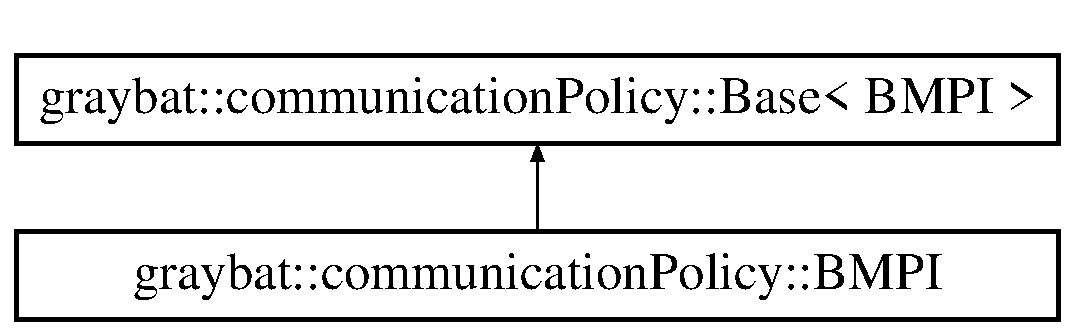
\includegraphics[height=2.000000cm]{structgraybat_1_1communicationPolicy_1_1BMPI}
\end{center}
\end{figure}
\subsection*{Public Types}
\begin{DoxyCompactItemize}
\item 
\hypertarget{structgraybat_1_1communicationPolicy_1_1BMPI_a8d250a80c1b23afea7da0aad7f008d00}{}using {\bfseries Tag} = typename graybat\+::communication\+Policy\+::\+Tag$<$ \hyperlink{structgraybat_1_1communicationPolicy_1_1BMPI}{B\+M\+P\+I} $>$\label{structgraybat_1_1communicationPolicy_1_1BMPI_a8d250a80c1b23afea7da0aad7f008d00}

\item 
\hypertarget{structgraybat_1_1communicationPolicy_1_1BMPI_a330e0f2f8ec3428af2ea9dd2d5695175}{}using {\bfseries Context\+I\+D} = typename graybat\+::communication\+Policy\+::\+Context\+I\+D$<$ \hyperlink{structgraybat_1_1communicationPolicy_1_1BMPI}{B\+M\+P\+I} $>$\label{structgraybat_1_1communicationPolicy_1_1BMPI_a330e0f2f8ec3428af2ea9dd2d5695175}

\item 
\hypertarget{structgraybat_1_1communicationPolicy_1_1BMPI_ac8cba626cca2151ace6a47bd0e51b64b}{}using {\bfseries Msg\+Type} = typename graybat\+::communication\+Policy\+::\+Msg\+Type$<$ \hyperlink{structgraybat_1_1communicationPolicy_1_1BMPI}{B\+M\+P\+I} $>$\label{structgraybat_1_1communicationPolicy_1_1BMPI_ac8cba626cca2151ace6a47bd0e51b64b}

\item 
\hypertarget{structgraybat_1_1communicationPolicy_1_1BMPI_ac214b2b6b3b852c387ebb3e3512555f2}{}using {\bfseries V\+Addr} = typename graybat\+::communication\+Policy\+::\+V\+Addr$<$ \hyperlink{structgraybat_1_1communicationPolicy_1_1BMPI}{B\+M\+P\+I} $>$\label{structgraybat_1_1communicationPolicy_1_1BMPI_ac214b2b6b3b852c387ebb3e3512555f2}

\item 
\hypertarget{structgraybat_1_1communicationPolicy_1_1BMPI_a571329de1fa15aa9e8fedcd9d70c6cb1}{}using {\bfseries Context} = typename graybat\+::communication\+Policy\+::\+Context$<$ \hyperlink{structgraybat_1_1communicationPolicy_1_1BMPI}{B\+M\+P\+I} $>$\label{structgraybat_1_1communicationPolicy_1_1BMPI_a571329de1fa15aa9e8fedcd9d70c6cb1}

\item 
\hypertarget{structgraybat_1_1communicationPolicy_1_1BMPI_afbdda3b27c1c7a556ea87368a0e02c3e}{}using {\bfseries Event} = typename graybat\+::communication\+Policy\+::\+Event$<$ \hyperlink{structgraybat_1_1communicationPolicy_1_1BMPI}{B\+M\+P\+I} $>$\label{structgraybat_1_1communicationPolicy_1_1BMPI_afbdda3b27c1c7a556ea87368a0e02c3e}

\item 
\hypertarget{structgraybat_1_1communicationPolicy_1_1BMPI_a38d4867df284c0642aa17cdefc68c676}{}using {\bfseries Config} = typename graybat\+::communication\+Policy\+::\+Config$<$ \hyperlink{structgraybat_1_1communicationPolicy_1_1BMPI}{B\+M\+P\+I} $>$\label{structgraybat_1_1communicationPolicy_1_1BMPI_a38d4867df284c0642aa17cdefc68c676}

\item 
\hypertarget{structgraybat_1_1communicationPolicy_1_1BMPI_a3dff8c14cca1780c399d51b7eb6df610}{}using {\bfseries Uri} = int\label{structgraybat_1_1communicationPolicy_1_1BMPI_a3dff8c14cca1780c399d51b7eb6df610}

\end{DoxyCompactItemize}
\subsection*{Public Member Functions}
\begin{DoxyCompactItemize}
\item 
\hypertarget{structgraybat_1_1communicationPolicy_1_1BMPI_a7f47c4f3521415aca2f6f6321b8bb87a}{}{\bfseries B\+M\+P\+I} (Config const config)\label{structgraybat_1_1communicationPolicy_1_1BMPI_a7f47c4f3521415aca2f6f6321b8bb87a}

\end{DoxyCompactItemize}
\begin{Indent}{\bf Point to Point Communication Interface}\par
\begin{DoxyCompactItemize}
\item 
{\footnotesize template$<$typename T\+\_\+\+Send $>$ }\\void \hyperlink{structgraybat_1_1communicationPolicy_1_1BMPI_a798111a6407368dc1b33b9893d9d1330}{send} (const V\+Addr dest\+V\+Addr, const \hyperlink{structTag}{Tag} tag, const Context context, const T\+\_\+\+Send \&send\+Data)
\begin{DoxyCompactList}\small\item\em Blocking transmission of a message send\+Data to peer with virtual address dest\+V\+Addr. \end{DoxyCompactList}\item 
{\footnotesize template$<$typename T\+\_\+\+Send $>$ }\\Event \hyperlink{structgraybat_1_1communicationPolicy_1_1BMPI_a68444513404ebd1548f34cbf3a2c3cc2}{async\+Send} (const V\+Addr dest\+V\+Addr, const \hyperlink{structTag}{Tag} tag, const Context context, const T\+\_\+\+Send \&send\+Data)
\begin{DoxyCompactList}\small\item\em Non blocking transmission of a message send\+Data to peer with virtual address dest\+V\+Addr. \end{DoxyCompactList}\item 
{\footnotesize template$<$typename T\+\_\+\+Recv $>$ }\\void \hyperlink{structgraybat_1_1communicationPolicy_1_1BMPI_a4201b53dcff9d3acef8724031d93a8fd}{recv} (const V\+Addr src\+V\+Addr, const \hyperlink{structTag}{Tag} tag, const Context context, T\+\_\+\+Recv \&recv\+Data)
\begin{DoxyCompactList}\small\item\em Blocking receive of a message recv\+Data from peer with virtual address src\+V\+Addr. \end{DoxyCompactList}\item 
\hypertarget{structgraybat_1_1communicationPolicy_1_1BMPI_a9b8346f1fab44e4160819a352f264884}{}{\footnotesize template$<$typename T\+\_\+\+Recv $>$ }\\Event {\bfseries recv} (const Context context, T\+\_\+\+Recv \&recv\+Data)\label{structgraybat_1_1communicationPolicy_1_1BMPI_a9b8346f1fab44e4160819a352f264884}

\item 
{\footnotesize template$<$typename T\+\_\+\+Recv $>$ }\\Event \hyperlink{structgraybat_1_1communicationPolicy_1_1BMPI_a092b709e200b44cacf32909e9dace56b}{async\+Recv} (const V\+Addr src\+V\+Addr, const \hyperlink{structTag}{Tag} tag, const Context context, T\+\_\+\+Recv \&recv\+Data)
\begin{DoxyCompactList}\small\item\em Non blocking receive of a message recv\+Data from peer with virtual address src\+V\+Addr. \end{DoxyCompactList}\end{DoxyCompactItemize}
\end{Indent}
\begin{Indent}{\bf Collective Communication Interface}\par
\begin{DoxyCompactItemize}
\item 
{\footnotesize template$<$typename T\+\_\+\+Send , typename T\+\_\+\+Recv $>$ }\\void \hyperlink{structgraybat_1_1communicationPolicy_1_1BMPI_a37fcb4dced08f33b4eee2adabf25fe0f}{gather} (const V\+Addr root\+V\+Addr, const Context context, const T\+\_\+\+Send \&send\+Data, T\+\_\+\+Recv \&recv\+Data)
\begin{DoxyCompactList}\small\item\em Collects {\itshape send\+Data} from all peers of the {\itshape context} and transmits it as a list to the peer with {\itshape root\+V\+Addr}. Data of all peers has to be from the {\bfseries same} size. \end{DoxyCompactList}\item 
{\footnotesize template$<$typename T\+\_\+\+Send , typename T\+\_\+\+Recv $>$ }\\void \hyperlink{structgraybat_1_1communicationPolicy_1_1BMPI_a772c45a8a2ec8ae749fef75ca2439cee}{gather\+Var} (const V\+Addr root\+V\+Addr, const Context context, const T\+\_\+\+Send \&send\+Data, T\+\_\+\+Recv \&recv\+Data, std\+::vector$<$ unsigned $>$ \&recv\+Count)
\begin{DoxyCompactList}\small\item\em Collects {\itshape send\+Data} from all members of the {\itshape context} with {\bfseries varying} size and transmits it as a list to peer with {\itshape root\+V\+Addr}. \end{DoxyCompactList}\item 
{\footnotesize template$<$typename T\+\_\+\+Send , typename T\+\_\+\+Recv $>$ }\\void \hyperlink{structgraybat_1_1communicationPolicy_1_1BMPI_abadfee42ac90516c1158292da79b0345}{all\+Gather} (Context context, const T\+\_\+\+Send \&send\+Data, T\+\_\+\+Recv \&recv\+Data)
\begin{DoxyCompactList}\small\item\em Collects {\itshape send\+Data} from all members of the {\itshape context} and transmits it as a list to every peer in the {\itshape context} \end{DoxyCompactList}\item 
{\footnotesize template$<$typename T\+\_\+\+Send , typename T\+\_\+\+Recv $>$ }\\void \hyperlink{structgraybat_1_1communicationPolicy_1_1BMPI_a0a365caf09acb118502623527c70668e}{all\+Gather\+Var} (const Context context, const T\+\_\+\+Send \&send\+Data, T\+\_\+\+Recv \&recv\+Data, std\+::vector$<$ unsigned $>$ \&recv\+Count)
\begin{DoxyCompactList}\small\item\em Collects {\itshape send\+Data} from all peers of the {\itshape context}. Size of {\itshape send\+Data} can vary in size. The data is received by every peer in the {\itshape context}. \end{DoxyCompactList}\item 
{\footnotesize template$<$typename T\+\_\+\+Send , typename T\+\_\+\+Recv $>$ }\\void \hyperlink{structgraybat_1_1communicationPolicy_1_1BMPI_ad1263d7d13beec1fe7267696c908d6eb}{scatter} (const V\+Addr root\+V\+Addr, const Context context, const T\+\_\+\+Send \&send\+Data, T\+\_\+\+Recv \&recv\+Data)
\begin{DoxyCompactList}\small\item\em Distributes {\itshape send\+Data} from peer {\itshape root\+V\+Addr} to all peers in {\itshape context}. Every peer will receive different data. \end{DoxyCompactList}\item 
{\footnotesize template$<$typename T\+\_\+\+Send , typename T\+\_\+\+Recv $>$ }\\void \hyperlink{structgraybat_1_1communicationPolicy_1_1BMPI_a1558d37c09b31ce63e7926f183515fa5}{all\+To\+All} (const Context context, const T\+\_\+\+Send \&send\+Data, T\+\_\+\+Recv \&recv\+Data)
\begin{DoxyCompactList}\small\item\em Distributes {\itshape send\+Data} of all peer in the {\itshape context} to all peers in the {\itshape context}. Every peer will receive data from every other peer (also the own data) \end{DoxyCompactList}\item 
{\footnotesize template$<$typename T\+\_\+\+Send , typename T\+\_\+\+Recv , typename T\+\_\+\+Op $>$ }\\void \hyperlink{structgraybat_1_1communicationPolicy_1_1BMPI_abee4b7a6d3026127cac5b25aa7d860f6}{reduce} (const V\+Addr root\+V\+Addr, const Context context, const T\+\_\+\+Op op, const T\+\_\+\+Send \&send\+Data, T\+\_\+\+Recv \&recv\+Data)
\begin{DoxyCompactList}\small\item\em Performs a reduction with a binary operator {\itshape op} on all {\itshape send\+Data} elements from all peers whithin the {\itshape context}. The result will be received by the peer with {\itshape root\+V\+Addr}. Binary operations like std\+::plus, std\+::minus can be used. But, they can also be defined as binary operator simular to std\+::plus etc. \end{DoxyCompactList}\item 
{\footnotesize template$<$typename T\+\_\+\+Send , typename T\+\_\+\+Recv , typename T\+\_\+\+Op $>$ }\\void \hyperlink{structgraybat_1_1communicationPolicy_1_1BMPI_aed0dd7f1c36157182cf0d0545879a6b8}{all\+Reduce} (const Context context, T\+\_\+\+Op op, const T\+\_\+\+Send \&send\+Data, T\+\_\+\+Recv \&recv\+Data)
\begin{DoxyCompactList}\small\item\em Performs a reduction with a binary operator {\itshape op} on all {\itshape send\+Data} elements from all peers whithin the {\itshape context}. The result will be received by all peers. \end{DoxyCompactList}\item 
{\footnotesize template$<$typename T\+\_\+\+Send\+Recv $>$ }\\void \hyperlink{structgraybat_1_1communicationPolicy_1_1BMPI_ad21dca81db3bd46870062ef978f00206}{broadcast} (const V\+Addr root\+V\+Addr, const Context context, T\+\_\+\+Send\+Recv \&data)
\begin{DoxyCompactList}\small\item\em Send {\itshape send\+Data} from peer {\itshape root\+V\+Addr} to all peers in {\itshape context}. Every peer will receive the same data. \end{DoxyCompactList}\item 
\hypertarget{structgraybat_1_1communicationPolicy_1_1BMPI_aa99355d8aae18e14c59b82c4ab4e2c29}{}void \hyperlink{structgraybat_1_1communicationPolicy_1_1BMPI_aa99355d8aae18e14c59b82c4ab4e2c29}{synchronize} (const Context context)\label{structgraybat_1_1communicationPolicy_1_1BMPI_aa99355d8aae18e14c59b82c4ab4e2c29}

\begin{DoxyCompactList}\small\item\em Synchronizes all peers within {\itshape context} to the same point in the programm execution (barrier). \end{DoxyCompactList}\item 
void \hyperlink{structgraybat_1_1communicationPolicy_1_1BMPI_ae2cb4b8fa14af3cd34fc4dd8c3af6baa}{synchronize} ()
\begin{DoxyCompactList}\small\item\em Synchronizes all peers within the global\+Context in the programm execution (barrier). \end{DoxyCompactList}\end{DoxyCompactItemize}
\end{Indent}
\begin{Indent}{\bf Context Management Interface}\par
\begin{DoxyCompactItemize}
\item 
\hypertarget{structgraybat_1_1communicationPolicy_1_1BMPI_a4c65002f731605e7e6d80acdc1d4c678}{}Context \hyperlink{structgraybat_1_1communicationPolicy_1_1BMPI_a4c65002f731605e7e6d80acdc1d4c678}{split\+Context} (const bool is\+Member, const Context old\+Context)\label{structgraybat_1_1communicationPolicy_1_1BMPI_a4c65002f731605e7e6d80acdc1d4c678}

\begin{DoxyCompactList}\small\item\em Creates a new context with all peers that declared is\+Member as true. \end{DoxyCompactList}\item 
\hypertarget{structgraybat_1_1communicationPolicy_1_1BMPI_aaaaaec7667d29a126cfc883cf552da31}{}Context \hyperlink{structgraybat_1_1communicationPolicy_1_1BMPI_aaaaaec7667d29a126cfc883cf552da31}{get\+Global\+Context} ()\label{structgraybat_1_1communicationPolicy_1_1BMPI_aaaaaec7667d29a126cfc883cf552da31}

\begin{DoxyCompactList}\small\item\em Returns the context that contains all peers. \end{DoxyCompactList}\end{DoxyCompactItemize}
\end{Indent}


\subsection{Detailed Description}
Implementation of the \hyperlink{structgraybat_1_1Cage}{Cage} communication\+Policy interface based on the M\+P\+I implementation boost\+::mpi. \begin{Desc}
\item[Examples\+: ]\par
\hyperlink{anyrecv_8cpp-example}{anyrecv.\+cpp}, \hyperlink{chain_8cpp-example}{chain.\+cpp}, \hyperlink{forward_8cpp-example}{forward.\+cpp}, \hyperlink{gol_8cpp-example}{gol.\+cpp}, and \hyperlink{ring_8cpp-example}{ring.\+cpp}.\end{Desc}


\subsection{Member Function Documentation}
\hypertarget{structgraybat_1_1communicationPolicy_1_1BMPI_abadfee42ac90516c1158292da79b0345}{}\index{graybat\+::communication\+Policy\+::\+B\+M\+P\+I@{graybat\+::communication\+Policy\+::\+B\+M\+P\+I}!all\+Gather@{all\+Gather}}
\index{all\+Gather@{all\+Gather}!graybat\+::communication\+Policy\+::\+B\+M\+P\+I@{graybat\+::communication\+Policy\+::\+B\+M\+P\+I}}
\subsubsection[{all\+Gather(\+Context context, const T\+\_\+\+Send \&send\+Data, T\+\_\+\+Recv \&recv\+Data)}]{\setlength{\rightskip}{0pt plus 5cm}template$<$typename T\+\_\+\+Send , typename T\+\_\+\+Recv $>$ void graybat\+::communication\+Policy\+::\+B\+M\+P\+I\+::all\+Gather (
\begin{DoxyParamCaption}
\item[{Context}]{context, }
\item[{const T\+\_\+\+Send \&}]{send\+Data, }
\item[{T\+\_\+\+Recv \&}]{recv\+Data}
\end{DoxyParamCaption}
)\hspace{0.3cm}{\ttfamily [inline]}}\label{structgraybat_1_1communicationPolicy_1_1BMPI_abadfee42ac90516c1158292da79b0345}


Collects {\itshape send\+Data} from all members of the {\itshape context} and transmits it as a list to every peer in the {\itshape context} 


\begin{DoxyParams}[1]{Parameters}
\mbox{\tt in}  & {\em context} & Set of peers that want to send Data \\
\hline
\mbox{\tt in}  & {\em send\+Data} & Data that every peer in the {\itshape context} sends with {\bfseries same} size \\
\hline
\mbox{\tt out}  & {\em recv\+Data} & Data from all {\itshape context} members, that all peers$\ast$ will receive. \\
\hline
\end{DoxyParams}
\hypertarget{structgraybat_1_1communicationPolicy_1_1BMPI_a0a365caf09acb118502623527c70668e}{}\index{graybat\+::communication\+Policy\+::\+B\+M\+P\+I@{graybat\+::communication\+Policy\+::\+B\+M\+P\+I}!all\+Gather\+Var@{all\+Gather\+Var}}
\index{all\+Gather\+Var@{all\+Gather\+Var}!graybat\+::communication\+Policy\+::\+B\+M\+P\+I@{graybat\+::communication\+Policy\+::\+B\+M\+P\+I}}
\subsubsection[{all\+Gather\+Var(const Context context, const T\+\_\+\+Send \&send\+Data, T\+\_\+\+Recv \&recv\+Data, std\+::vector$<$ unsigned $>$ \&recv\+Count)}]{\setlength{\rightskip}{0pt plus 5cm}template$<$typename T\+\_\+\+Send , typename T\+\_\+\+Recv $>$ void graybat\+::communication\+Policy\+::\+B\+M\+P\+I\+::all\+Gather\+Var (
\begin{DoxyParamCaption}
\item[{const Context}]{context, }
\item[{const T\+\_\+\+Send \&}]{send\+Data, }
\item[{T\+\_\+\+Recv \&}]{recv\+Data, }
\item[{std\+::vector$<$ unsigned $>$ \&}]{recv\+Count}
\end{DoxyParamCaption}
)\hspace{0.3cm}{\ttfamily [inline]}}\label{structgraybat_1_1communicationPolicy_1_1BMPI_a0a365caf09acb118502623527c70668e}


Collects {\itshape send\+Data} from all peers of the {\itshape context}. Size of {\itshape send\+Data} can vary in size. The data is received by every peer in the {\itshape context}. 


\begin{DoxyParams}[1]{Parameters}
\mbox{\tt in}  & {\em context} & Set of peers that want to send Data \\
\hline
\mbox{\tt in}  & {\em send\+Data} & Data that every peer in the {\itshape context} sends with {\bfseries varying} size \\
\hline
\mbox{\tt out}  & {\em recv\+Data} & Data from all {\itshape context} members, that all peers$\ast$ will receive. \\
\hline
\mbox{\tt out}  & {\em recv\+Count} & Number of elements each peer sends (can by varying). \\
\hline
\end{DoxyParams}
\hypertarget{structgraybat_1_1communicationPolicy_1_1BMPI_aed0dd7f1c36157182cf0d0545879a6b8}{}\index{graybat\+::communication\+Policy\+::\+B\+M\+P\+I@{graybat\+::communication\+Policy\+::\+B\+M\+P\+I}!all\+Reduce@{all\+Reduce}}
\index{all\+Reduce@{all\+Reduce}!graybat\+::communication\+Policy\+::\+B\+M\+P\+I@{graybat\+::communication\+Policy\+::\+B\+M\+P\+I}}
\subsubsection[{all\+Reduce(const Context context, T\+\_\+\+Op op, const T\+\_\+\+Send \&send\+Data, T\+\_\+\+Recv \&recv\+Data)}]{\setlength{\rightskip}{0pt plus 5cm}template$<$typename T\+\_\+\+Send , typename T\+\_\+\+Recv , typename T\+\_\+\+Op $>$ void graybat\+::communication\+Policy\+::\+B\+M\+P\+I\+::all\+Reduce (
\begin{DoxyParamCaption}
\item[{const Context}]{context, }
\item[{T\+\_\+\+Op}]{op, }
\item[{const T\+\_\+\+Send \&}]{send\+Data, }
\item[{T\+\_\+\+Recv \&}]{recv\+Data}
\end{DoxyParamCaption}
)\hspace{0.3cm}{\ttfamily [inline]}}\label{structgraybat_1_1communicationPolicy_1_1BMPI_aed0dd7f1c36157182cf0d0545879a6b8}


Performs a reduction with a binary operator {\itshape op} on all {\itshape send\+Data} elements from all peers whithin the {\itshape context}. The result will be received by all peers. 


\begin{DoxyParams}[1]{Parameters}
\mbox{\tt in}  & {\em context} & Set of peers that \\
\hline
\mbox{\tt in}  & {\em op} & Binary operator that should be used for reduction \\
\hline
\mbox{\tt in}  & {\em send\+Data} & Data that every peer contributes to the reduction \\
\hline
\mbox{\tt out}  & {\em recv\+Data} & Reduced send\+Data that will be received by all peers. It will have same size of send\+Data and contains the ith reduced send\+Data values. \\
\hline
\end{DoxyParams}
\hypertarget{structgraybat_1_1communicationPolicy_1_1BMPI_a1558d37c09b31ce63e7926f183515fa5}{}\index{graybat\+::communication\+Policy\+::\+B\+M\+P\+I@{graybat\+::communication\+Policy\+::\+B\+M\+P\+I}!all\+To\+All@{all\+To\+All}}
\index{all\+To\+All@{all\+To\+All}!graybat\+::communication\+Policy\+::\+B\+M\+P\+I@{graybat\+::communication\+Policy\+::\+B\+M\+P\+I}}
\subsubsection[{all\+To\+All(const Context context, const T\+\_\+\+Send \&send\+Data, T\+\_\+\+Recv \&recv\+Data)}]{\setlength{\rightskip}{0pt plus 5cm}template$<$typename T\+\_\+\+Send , typename T\+\_\+\+Recv $>$ void graybat\+::communication\+Policy\+::\+B\+M\+P\+I\+::all\+To\+All (
\begin{DoxyParamCaption}
\item[{const Context}]{context, }
\item[{const T\+\_\+\+Send \&}]{send\+Data, }
\item[{T\+\_\+\+Recv \&}]{recv\+Data}
\end{DoxyParamCaption}
)\hspace{0.3cm}{\ttfamily [inline]}}\label{structgraybat_1_1communicationPolicy_1_1BMPI_a1558d37c09b31ce63e7926f183515fa5}


Distributes {\itshape send\+Data} of all peer in the {\itshape context} to all peers in the {\itshape context}. Every peer will receive data from every other peer (also the own data) 


\begin{DoxyParams}[1]{Parameters}
\mbox{\tt in}  & {\em context} & Set of peers that want to receive Data \\
\hline
\mbox{\tt in}  & {\em send\+Data} & Data that each peer wants to send. Each peer will receive same number of data elements, but not the same data elements. send\+Data will be divided in equal chunks of data and is then distributed.\\
\hline
\mbox{\tt out}  & {\em recv\+Data} & Data from all peer. \\
\hline
\end{DoxyParams}
\hypertarget{structgraybat_1_1communicationPolicy_1_1BMPI_a092b709e200b44cacf32909e9dace56b}{}\index{graybat\+::communication\+Policy\+::\+B\+M\+P\+I@{graybat\+::communication\+Policy\+::\+B\+M\+P\+I}!async\+Recv@{async\+Recv}}
\index{async\+Recv@{async\+Recv}!graybat\+::communication\+Policy\+::\+B\+M\+P\+I@{graybat\+::communication\+Policy\+::\+B\+M\+P\+I}}
\subsubsection[{async\+Recv(const V\+Addr src\+V\+Addr, const Tag tag, const Context context, T\+\_\+\+Recv \&recv\+Data)}]{\setlength{\rightskip}{0pt plus 5cm}template$<$typename T\+\_\+\+Recv $>$ Event graybat\+::communication\+Policy\+::\+B\+M\+P\+I\+::async\+Recv (
\begin{DoxyParamCaption}
\item[{const V\+Addr}]{src\+V\+Addr, }
\item[{const {\bf Tag}}]{tag, }
\item[{const Context}]{context, }
\item[{T\+\_\+\+Recv \&}]{recv\+Data}
\end{DoxyParamCaption}
)\hspace{0.3cm}{\ttfamily [inline]}}\label{structgraybat_1_1communicationPolicy_1_1BMPI_a092b709e200b44cacf32909e9dace56b}


Non blocking receive of a message recv\+Data from peer with virtual address src\+V\+Addr. 


\begin{DoxyParams}[1]{Parameters}
\mbox{\tt in}  & {\em src\+V\+Addr} & V\+Addr of peer that sended the message \\
\hline
\mbox{\tt in}  & {\em tag} & Description of the message to better distinguish messages types \\
\hline
\mbox{\tt in}  & {\em context} & Context in which both sender and receiver are included \\
\hline
\mbox{\tt out}  & {\em recv\+Data} & Data reference of template type T will be received from sender peer. T need to provide the function data(), that returns the pointer to the data memory address. And the function size(), that return the amount of data elements to send. Notice, that std\+::vector and std\+::array implement this interface.\\
\hline
\end{DoxyParams}
\begin{DoxyReturn}{Returns}
Event 
\end{DoxyReturn}
\hypertarget{structgraybat_1_1communicationPolicy_1_1BMPI_a68444513404ebd1548f34cbf3a2c3cc2}{}\index{graybat\+::communication\+Policy\+::\+B\+M\+P\+I@{graybat\+::communication\+Policy\+::\+B\+M\+P\+I}!async\+Send@{async\+Send}}
\index{async\+Send@{async\+Send}!graybat\+::communication\+Policy\+::\+B\+M\+P\+I@{graybat\+::communication\+Policy\+::\+B\+M\+P\+I}}
\subsubsection[{async\+Send(const V\+Addr dest\+V\+Addr, const Tag tag, const Context context, const T\+\_\+\+Send \&send\+Data)}]{\setlength{\rightskip}{0pt plus 5cm}template$<$typename T\+\_\+\+Send $>$ Event graybat\+::communication\+Policy\+::\+B\+M\+P\+I\+::async\+Send (
\begin{DoxyParamCaption}
\item[{const V\+Addr}]{dest\+V\+Addr, }
\item[{const {\bf Tag}}]{tag, }
\item[{const Context}]{context, }
\item[{const T\+\_\+\+Send \&}]{send\+Data}
\end{DoxyParamCaption}
)\hspace{0.3cm}{\ttfamily [inline]}}\label{structgraybat_1_1communicationPolicy_1_1BMPI_a68444513404ebd1548f34cbf3a2c3cc2}


Non blocking transmission of a message send\+Data to peer with virtual address dest\+V\+Addr. 


\begin{DoxyParams}[1]{Parameters}
\mbox{\tt in}  & {\em dest\+V\+Addr} & V\+Addr of peer that will receive the message \\
\hline
\mbox{\tt in}  & {\em tag} & Description of the message to better distinguish messages types \\
\hline
\mbox{\tt in}  & {\em context} & Context in which both sender and receiver are included \\
\hline
\mbox{\tt in}  & {\em send\+Data} & Data reference of template type T will be. T need to provide the function data(), that returns the pointer to the data memory address. And the function size(), that return the amount of data elements to send. Notice, that std\+::vector and std\+::array implement this interface.\\
\hline
\end{DoxyParams}
\begin{DoxyReturn}{Returns}
Event 
\end{DoxyReturn}
\hypertarget{structgraybat_1_1communicationPolicy_1_1BMPI_ad21dca81db3bd46870062ef978f00206}{}\index{graybat\+::communication\+Policy\+::\+B\+M\+P\+I@{graybat\+::communication\+Policy\+::\+B\+M\+P\+I}!broadcast@{broadcast}}
\index{broadcast@{broadcast}!graybat\+::communication\+Policy\+::\+B\+M\+P\+I@{graybat\+::communication\+Policy\+::\+B\+M\+P\+I}}
\subsubsection[{broadcast(const V\+Addr root\+V\+Addr, const Context context, T\+\_\+\+Send\+Recv \&data)}]{\setlength{\rightskip}{0pt plus 5cm}template$<$typename T\+\_\+\+Send\+Recv $>$ void graybat\+::communication\+Policy\+::\+B\+M\+P\+I\+::broadcast (
\begin{DoxyParamCaption}
\item[{const V\+Addr}]{root\+V\+Addr, }
\item[{const Context}]{context, }
\item[{T\+\_\+\+Send\+Recv \&}]{data}
\end{DoxyParamCaption}
)\hspace{0.3cm}{\ttfamily [inline]}}\label{structgraybat_1_1communicationPolicy_1_1BMPI_ad21dca81db3bd46870062ef978f00206}


Send {\itshape send\+Data} from peer {\itshape root\+V\+Addr} to all peers in {\itshape context}. Every peer will receive the same data. 

\begin{DoxyRemark}{Remarks}
In Contrast to scatter where every peer receives different data
\end{DoxyRemark}

\begin{DoxyParams}[1]{Parameters}
\mbox{\tt in}  & {\em root\+V\+Addr} & Source peer \\
\hline
\mbox{\tt in}  & {\em context} & Set of peers that want to receive Data \\
\hline
\mbox{\tt in}  & {\em send\+Data} & Data that peer with {\itshape root\+V\+Addr} will send to the peers of the {\itshape context} \\
\hline
\mbox{\tt out}  & {\em recv\+Data} & Data from peer with {\itshape root\+V\+Addr}. \\
\hline
\end{DoxyParams}
\hypertarget{structgraybat_1_1communicationPolicy_1_1BMPI_a37fcb4dced08f33b4eee2adabf25fe0f}{}\index{graybat\+::communication\+Policy\+::\+B\+M\+P\+I@{graybat\+::communication\+Policy\+::\+B\+M\+P\+I}!gather@{gather}}
\index{gather@{gather}!graybat\+::communication\+Policy\+::\+B\+M\+P\+I@{graybat\+::communication\+Policy\+::\+B\+M\+P\+I}}
\subsubsection[{gather(const V\+Addr root\+V\+Addr, const Context context, const T\+\_\+\+Send \&send\+Data, T\+\_\+\+Recv \&recv\+Data)}]{\setlength{\rightskip}{0pt plus 5cm}template$<$typename T\+\_\+\+Send , typename T\+\_\+\+Recv $>$ void graybat\+::communication\+Policy\+::\+B\+M\+P\+I\+::gather (
\begin{DoxyParamCaption}
\item[{const V\+Addr}]{root\+V\+Addr, }
\item[{const Context}]{context, }
\item[{const T\+\_\+\+Send \&}]{send\+Data, }
\item[{T\+\_\+\+Recv \&}]{recv\+Data}
\end{DoxyParamCaption}
)\hspace{0.3cm}{\ttfamily [inline]}}\label{structgraybat_1_1communicationPolicy_1_1BMPI_a37fcb4dced08f33b4eee2adabf25fe0f}


Collects {\itshape send\+Data} from all peers of the {\itshape context} and transmits it as a list to the peer with {\itshape root\+V\+Addr}. Data of all peers has to be from the {\bfseries same} size. 


\begin{DoxyParams}[1]{Parameters}
\mbox{\tt in}  & {\em root\+V\+Addr} & Peer that will receive collcted data from {\itshape context} members \\
\hline
\mbox{\tt in}  & {\em context} & Set of peers that want to send Data \\
\hline
\mbox{\tt in}  & {\em send\+Data} & Data that every peer in the {\itshape context} sends. Data of all peers in the {\itshape context} need to have {\bfseries same} size(). \\
\hline
\mbox{\tt out}  & {\em recv\+Data} & Data from all {\itshape context} members, that peer with virtual address {\itshape root\+V\+Addr} will receive. {\itshape recv\+Data} of all other members of the {\itshape context} will be empty. \\
\hline
\end{DoxyParams}
\hypertarget{structgraybat_1_1communicationPolicy_1_1BMPI_a772c45a8a2ec8ae749fef75ca2439cee}{}\index{graybat\+::communication\+Policy\+::\+B\+M\+P\+I@{graybat\+::communication\+Policy\+::\+B\+M\+P\+I}!gather\+Var@{gather\+Var}}
\index{gather\+Var@{gather\+Var}!graybat\+::communication\+Policy\+::\+B\+M\+P\+I@{graybat\+::communication\+Policy\+::\+B\+M\+P\+I}}
\subsubsection[{gather\+Var(const V\+Addr root\+V\+Addr, const Context context, const T\+\_\+\+Send \&send\+Data, T\+\_\+\+Recv \&recv\+Data, std\+::vector$<$ unsigned $>$ \&recv\+Count)}]{\setlength{\rightskip}{0pt plus 5cm}template$<$typename T\+\_\+\+Send , typename T\+\_\+\+Recv $>$ void graybat\+::communication\+Policy\+::\+B\+M\+P\+I\+::gather\+Var (
\begin{DoxyParamCaption}
\item[{const V\+Addr}]{root\+V\+Addr, }
\item[{const Context}]{context, }
\item[{const T\+\_\+\+Send \&}]{send\+Data, }
\item[{T\+\_\+\+Recv \&}]{recv\+Data, }
\item[{std\+::vector$<$ unsigned $>$ \&}]{recv\+Count}
\end{DoxyParamCaption}
)\hspace{0.3cm}{\ttfamily [inline]}}\label{structgraybat_1_1communicationPolicy_1_1BMPI_a772c45a8a2ec8ae749fef75ca2439cee}


Collects {\itshape send\+Data} from all members of the {\itshape context} with {\bfseries varying} size and transmits it as a list to peer with {\itshape root\+V\+Addr}. 


\begin{DoxyParams}[1]{Parameters}
\mbox{\tt in}  & {\em root\+V\+Addr} & Peer that will receive collcted data from {\itshape context} members \\
\hline
\mbox{\tt in}  & {\em context} & Set of peers that want to send Data \\
\hline
\mbox{\tt in}  & {\em send\+Data} & Data that every peer in the {\itshape context} sends. The Data can have {\bfseries varying} size \\
\hline
\mbox{\tt out}  & {\em recv\+Data} & Data from all {\itshape context} peers, that peer with {\itshape root\+V\+Addr} will receive. {\itshape recv\+Data} of all other peers of the {\itshape context} will be empty. The received data is ordered by the V\+Addr of the peers. \\
\hline
\mbox{\tt out}  & {\em recv\+Count} & Number of elements each peer sends (can by varying). \\
\hline
\end{DoxyParams}
\hypertarget{structgraybat_1_1communicationPolicy_1_1BMPI_a4201b53dcff9d3acef8724031d93a8fd}{}\index{graybat\+::communication\+Policy\+::\+B\+M\+P\+I@{graybat\+::communication\+Policy\+::\+B\+M\+P\+I}!recv@{recv}}
\index{recv@{recv}!graybat\+::communication\+Policy\+::\+B\+M\+P\+I@{graybat\+::communication\+Policy\+::\+B\+M\+P\+I}}
\subsubsection[{recv(const V\+Addr src\+V\+Addr, const Tag tag, const Context context, T\+\_\+\+Recv \&recv\+Data)}]{\setlength{\rightskip}{0pt plus 5cm}template$<$typename T\+\_\+\+Recv $>$ void graybat\+::communication\+Policy\+::\+B\+M\+P\+I\+::recv (
\begin{DoxyParamCaption}
\item[{const V\+Addr}]{src\+V\+Addr, }
\item[{const {\bf Tag}}]{tag, }
\item[{const Context}]{context, }
\item[{T\+\_\+\+Recv \&}]{recv\+Data}
\end{DoxyParamCaption}
)\hspace{0.3cm}{\ttfamily [inline]}}\label{structgraybat_1_1communicationPolicy_1_1BMPI_a4201b53dcff9d3acef8724031d93a8fd}


Blocking receive of a message recv\+Data from peer with virtual address src\+V\+Addr. 


\begin{DoxyParams}[1]{Parameters}
\mbox{\tt in}  & {\em src\+V\+Addr} & V\+Addr of peer that sended the message \\
\hline
\mbox{\tt in}  & {\em tag} & Description of the message to better distinguish messages types \\
\hline
\mbox{\tt in}  & {\em context} & Context in which both sender and receiver are included \\
\hline
\mbox{\tt out}  & {\em recv\+Data} & Data reference of template type T will be received from sender peer. T need to provide the function data(), that returns the pointer to the data memory address. And the function size(), that return the amount of data elements to send. Notice, that std\+::vector and std\+::array implement this interface. \\
\hline
\end{DoxyParams}
\hypertarget{structgraybat_1_1communicationPolicy_1_1BMPI_abee4b7a6d3026127cac5b25aa7d860f6}{}\index{graybat\+::communication\+Policy\+::\+B\+M\+P\+I@{graybat\+::communication\+Policy\+::\+B\+M\+P\+I}!reduce@{reduce}}
\index{reduce@{reduce}!graybat\+::communication\+Policy\+::\+B\+M\+P\+I@{graybat\+::communication\+Policy\+::\+B\+M\+P\+I}}
\subsubsection[{reduce(const V\+Addr root\+V\+Addr, const Context context, const T\+\_\+\+Op op, const T\+\_\+\+Send \&send\+Data, T\+\_\+\+Recv \&recv\+Data)}]{\setlength{\rightskip}{0pt plus 5cm}template$<$typename T\+\_\+\+Send , typename T\+\_\+\+Recv , typename T\+\_\+\+Op $>$ void graybat\+::communication\+Policy\+::\+B\+M\+P\+I\+::reduce (
\begin{DoxyParamCaption}
\item[{const V\+Addr}]{root\+V\+Addr, }
\item[{const Context}]{context, }
\item[{const T\+\_\+\+Op}]{op, }
\item[{const T\+\_\+\+Send \&}]{send\+Data, }
\item[{T\+\_\+\+Recv \&}]{recv\+Data}
\end{DoxyParamCaption}
)\hspace{0.3cm}{\ttfamily [inline]}}\label{structgraybat_1_1communicationPolicy_1_1BMPI_abee4b7a6d3026127cac5b25aa7d860f6}


Performs a reduction with a binary operator {\itshape op} on all {\itshape send\+Data} elements from all peers whithin the {\itshape context}. The result will be received by the peer with {\itshape root\+V\+Addr}. Binary operations like std\+::plus, std\+::minus can be used. But, they can also be defined as binary operator simular to std\+::plus etc. 


\begin{DoxyParams}[1]{Parameters}
\mbox{\tt in}  & {\em root\+V\+Addr} & peer that will receive the result of reduction \\
\hline
\mbox{\tt in}  & {\em context} & Set of peers that \\
\hline
\mbox{\tt in}  & {\em op} & Binary operator that should be used for reduction \\
\hline
\mbox{\tt in}  & {\em send\+Data} & Data that every peer contributes to the reduction \\
\hline
\mbox{\tt out}  & {\em recv\+Data} & Reduced send\+Data that will be received by peer with {\itshape root\+V\+Addr}. It will have same size of send\+Data and contains the ith reduced send\+Data values. \\
\hline
\end{DoxyParams}
\hypertarget{structgraybat_1_1communicationPolicy_1_1BMPI_ad1263d7d13beec1fe7267696c908d6eb}{}\index{graybat\+::communication\+Policy\+::\+B\+M\+P\+I@{graybat\+::communication\+Policy\+::\+B\+M\+P\+I}!scatter@{scatter}}
\index{scatter@{scatter}!graybat\+::communication\+Policy\+::\+B\+M\+P\+I@{graybat\+::communication\+Policy\+::\+B\+M\+P\+I}}
\subsubsection[{scatter(const V\+Addr root\+V\+Addr, const Context context, const T\+\_\+\+Send \&send\+Data, T\+\_\+\+Recv \&recv\+Data)}]{\setlength{\rightskip}{0pt plus 5cm}template$<$typename T\+\_\+\+Send , typename T\+\_\+\+Recv $>$ void graybat\+::communication\+Policy\+::\+B\+M\+P\+I\+::scatter (
\begin{DoxyParamCaption}
\item[{const V\+Addr}]{root\+V\+Addr, }
\item[{const Context}]{context, }
\item[{const T\+\_\+\+Send \&}]{send\+Data, }
\item[{T\+\_\+\+Recv \&}]{recv\+Data}
\end{DoxyParamCaption}
)\hspace{0.3cm}{\ttfamily [inline]}}\label{structgraybat_1_1communicationPolicy_1_1BMPI_ad1263d7d13beec1fe7267696c908d6eb}


Distributes {\itshape send\+Data} from peer {\itshape root\+V\+Addr} to all peers in {\itshape context}. Every peer will receive different data. 

\begin{DoxyRemark}{Remarks}
In Contrast to broadcast where every peer receives the same data
\end{DoxyRemark}

\begin{DoxyParams}[1]{Parameters}
\mbox{\tt in}  & {\em root\+V\+Addr} & peer that want to distribute its data \\
\hline
\mbox{\tt in}  & {\em context} & Set of peers that want to receive Data \\
\hline
\mbox{\tt in}  & {\em send\+Data} & Data that peer with {\itshape root\+V\+Addr} will distribute over the peers of the {\itshape context} \\
\hline
\mbox{\tt out}  & {\em recv\+Data} & Data from peer with {\itshape root\+V\+Addr}. \\
\hline
\end{DoxyParams}
\hypertarget{structgraybat_1_1communicationPolicy_1_1BMPI_a798111a6407368dc1b33b9893d9d1330}{}\index{graybat\+::communication\+Policy\+::\+B\+M\+P\+I@{graybat\+::communication\+Policy\+::\+B\+M\+P\+I}!send@{send}}
\index{send@{send}!graybat\+::communication\+Policy\+::\+B\+M\+P\+I@{graybat\+::communication\+Policy\+::\+B\+M\+P\+I}}
\subsubsection[{send(const V\+Addr dest\+V\+Addr, const Tag tag, const Context context, const T\+\_\+\+Send \&send\+Data)}]{\setlength{\rightskip}{0pt plus 5cm}template$<$typename T\+\_\+\+Send $>$ void graybat\+::communication\+Policy\+::\+B\+M\+P\+I\+::send (
\begin{DoxyParamCaption}
\item[{const V\+Addr}]{dest\+V\+Addr, }
\item[{const {\bf Tag}}]{tag, }
\item[{const Context}]{context, }
\item[{const T\+\_\+\+Send \&}]{send\+Data}
\end{DoxyParamCaption}
)\hspace{0.3cm}{\ttfamily [inline]}}\label{structgraybat_1_1communicationPolicy_1_1BMPI_a798111a6407368dc1b33b9893d9d1330}


Blocking transmission of a message send\+Data to peer with virtual address dest\+V\+Addr. 


\begin{DoxyParams}[1]{Parameters}
\mbox{\tt in}  & {\em dest\+V\+Addr} & V\+Addr of peer that will receive the message \\
\hline
\mbox{\tt in}  & {\em tag} & Description of the message to better distinguish messages types \\
\hline
\mbox{\tt in}  & {\em context} & Context in which both sender and receiver are included \\
\hline
\mbox{\tt in}  & {\em send\+Data} & Data reference of template type T will be send to receiver peer. T need to provide the function data(), that returns the pointer to the data memory address. And the function size(), that return the amount of data elements to send. Notice, that std\+::vector and std\+::array implement this interface. \\
\hline
\end{DoxyParams}
\hypertarget{structgraybat_1_1communicationPolicy_1_1BMPI_ae2cb4b8fa14af3cd34fc4dd8c3af6baa}{}\index{graybat\+::communication\+Policy\+::\+B\+M\+P\+I@{graybat\+::communication\+Policy\+::\+B\+M\+P\+I}!synchronize@{synchronize}}
\index{synchronize@{synchronize}!graybat\+::communication\+Policy\+::\+B\+M\+P\+I@{graybat\+::communication\+Policy\+::\+B\+M\+P\+I}}
\subsubsection[{synchronize()}]{\setlength{\rightskip}{0pt plus 5cm}void graybat\+::communication\+Policy\+::\+B\+M\+P\+I\+::synchronize (
\begin{DoxyParamCaption}
{}
\end{DoxyParamCaption}
)\hspace{0.3cm}{\ttfamily [inline]}}\label{structgraybat_1_1communicationPolicy_1_1BMPI_ae2cb4b8fa14af3cd34fc4dd8c3af6baa}


Synchronizes all peers within the global\+Context in the programm execution (barrier). 

\begin{DoxySeeAlso}{See also}
\hyperlink{structgraybat_1_1communicationPolicy_1_1BMPI_aaaaaec7667d29a126cfc883cf552da31}{get\+Global\+Context()} 
\end{DoxySeeAlso}


The documentation for this class was generated from the following file\+:\begin{DoxyCompactItemize}
\item 
include/graybat/communication\+Policy/B\+M\+P\+I.\+hpp\end{DoxyCompactItemize}

\hypertarget{structgraybat_1_1Cage}{}\section{graybat\+:\+:Cage$<$ T\+\_\+\+Communication\+Policy, T\+\_\+\+Graph\+Policy $>$ Class Template Reference}
\label{structgraybat_1_1Cage}\index{graybat\+::\+Cage$<$ T\+\_\+\+Communication\+Policy, T\+\_\+\+Graph\+Policy $>$@{graybat\+::\+Cage$<$ T\+\_\+\+Communication\+Policy, T\+\_\+\+Graph\+Policy $>$}}


The Communication And Graph Environment enables to communicate on basis of a graph with methods of a user defined communication library.  




{\ttfamily \#include $<$Cage.\+hpp$>$}

\subsection*{Classes}
\begin{DoxyCompactItemize}
\item 
struct \hyperlink{structgraybat_1_1Cage_1_1maximum}{maximum}
\end{DoxyCompactItemize}
\subsection*{Public Types}
\begin{DoxyCompactItemize}
\item 
\hypertarget{structgraybat_1_1Cage_a848caea3a16ff2390c8b0020cef298f2}{}using {\bfseries Communication\+Policy} = T\+\_\+\+Communication\+Policy\label{structgraybat_1_1Cage_a848caea3a16ff2390c8b0020cef298f2}

\item 
\hypertarget{structgraybat_1_1Cage_afc98171db17598bd0030d90ff101e4c2}{}using {\bfseries Graph\+Policy} = T\+\_\+\+Graph\+Policy\label{structgraybat_1_1Cage_afc98171db17598bd0030d90ff101e4c2}

\item 
\hypertarget{structgraybat_1_1Cage_ac7de84bd47f0af51bf87051355424ce9}{}using {\bfseries Cage\+\_\+t} = \hyperlink{structgraybat_1_1Cage}{Cage}$<$ Communication\+Policy, Graph\+Policy $>$\label{structgraybat_1_1Cage_ac7de84bd47f0af51bf87051355424ce9}

\item 
\hypertarget{structgraybat_1_1Cage_a5fcd15bbd715221a9d05f2fa5f2d14d5}{}using {\bfseries V\+Addr} = graybat\+::communication\+Policy\+::\+V\+Addr$<$ Communication\+Policy $>$\label{structgraybat_1_1Cage_a5fcd15bbd715221a9d05f2fa5f2d14d5}

\item 
\hypertarget{structgraybat_1_1Cage_a716c512829be5cca5dcbf2a52754d10d}{}using {\bfseries Context} = graybat\+::communication\+Policy\+::\+Context$<$ Communication\+Policy $>$\label{structgraybat_1_1Cage_a716c512829be5cca5dcbf2a52754d10d}

\item 
\hypertarget{structgraybat_1_1Cage_af23858450f27e9dfde241521a13df525}{}using {\bfseries Event} = graybat\+::communication\+Policy\+::\+Event$<$ Communication\+Policy $>$\label{structgraybat_1_1Cage_af23858450f27e9dfde241521a13df525}

\item 
\hypertarget{structgraybat_1_1Cage_a425d340120d20ee287043cbaa3e66d27}{}using {\bfseries C\+P\+Config} = graybat\+::communication\+Policy\+::\+Config$<$ Communication\+Policy $>$\label{structgraybat_1_1Cage_a425d340120d20ee287043cbaa3e66d27}

\item 
\hypertarget{structgraybat_1_1Cage_a1c8a9c50bfa2ac05eb0e36acf2c4f791}{}using {\bfseries Edge} = \hyperlink{structgraybat_1_1CommunicationEdge}{graybat\+::\+Communication\+Edge}$<$ \hyperlink{structgraybat_1_1Cage}{Cage\+\_\+t} $>$\label{structgraybat_1_1Cage_a1c8a9c50bfa2ac05eb0e36acf2c4f791}

\item 
\hypertarget{structgraybat_1_1Cage_acfd9a202873f8a3d1cc5680bc2ac9267}{}using {\bfseries Vertex} = \hyperlink{structgraybat_1_1CommunicationVertex}{graybat\+::\+Communication\+Vertex}$<$ \hyperlink{structgraybat_1_1Cage}{Cage\+\_\+t} $>$\label{structgraybat_1_1Cage_acfd9a202873f8a3d1cc5680bc2ac9267}

\item 
\hypertarget{structgraybat_1_1Cage_ae6c3a8d91a9e19c48b760216646b07e3}{}using {\bfseries Edge\+Description} = graybat\+::graph\+Policy\+::\+Edge\+Description$<$ Graph\+Policy $>$\label{structgraybat_1_1Cage_ae6c3a8d91a9e19c48b760216646b07e3}

\item 
\hypertarget{structgraybat_1_1Cage_a8dcd6874d2fbb5a2a731f197aedcb87f}{}using {\bfseries Graph\+Description} = graybat\+::graph\+Policy\+::\+Graph\+Description$<$ Graph\+Policy $>$\label{structgraybat_1_1Cage_a8dcd6874d2fbb5a2a731f197aedcb87f}

\item 
\hypertarget{structgraybat_1_1Cage_ad1ae456d67c2804c63a3d651096ec2c8}{}using {\bfseries Vertex\+I\+D} = graybat\+::graph\+Policy\+::\+Vertex\+I\+D\label{structgraybat_1_1Cage_ad1ae456d67c2804c63a3d651096ec2c8}

\item 
\hypertarget{structgraybat_1_1Cage_af7f17dd2b92c84abe4b9d49b2ae6f475}{}using {\bfseries Edge\+I\+D} = graybat\+::graph\+Policy\+::\+Edge\+I\+D\label{structgraybat_1_1Cage_af7f17dd2b92c84abe4b9d49b2ae6f475}

\item 
\hypertarget{structgraybat_1_1Cage_af763549ebaa29f10a5c72246c81a8c5d}{}using {\bfseries Graph\+I\+D} = graybat\+::graph\+Policy\+::\+Graph\+I\+D\label{structgraybat_1_1Cage_af763549ebaa29f10a5c72246c81a8c5d}

\item 
\hypertarget{structgraybat_1_1Cage_abcd2ec48a85543b8521fd85ed7dd1927}{}using {\bfseries Peer} = size\+\_\+t\label{structgraybat_1_1Cage_abcd2ec48a85543b8521fd85ed7dd1927}

\end{DoxyCompactItemize}
\subsection*{Public Member Functions}
\begin{DoxyCompactItemize}
\item 
\hypertarget{structgraybat_1_1Cage_a4a5b4f29c8fef120674b95ac25f05518}{}{\footnotesize template$<$class T\+\_\+\+Functor $>$ }\\{\bfseries Cage} (C\+P\+Config const cp\+Config, T\+\_\+\+Functor graph\+Functor)\label{structgraybat_1_1Cage_a4a5b4f29c8fef120674b95ac25f05518}

\item 
\hypertarget{structgraybat_1_1Cage_a9e76d7d8a6dddbb5fbf6882506f80ab1}{}{\bfseries Cage} (C\+P\+Config const cp\+Config)\label{structgraybat_1_1Cage_a9e76d7d8a6dddbb5fbf6882506f80ab1}

\end{DoxyCompactItemize}
\begin{Indent}{\bf Graph Operations}\par
\begin{DoxyCompactItemize}
\item 
\hypertarget{structgraybat_1_1Cage_adeb898f46486654a94ee8198d31272fb}{}{\footnotesize template$<$class T\+\_\+\+Functor $>$ }\\void {\bfseries set\+Graph} (T\+\_\+\+Functor graph\+Functor)\label{structgraybat_1_1Cage_adeb898f46486654a94ee8198d31272fb}

\item 
\hypertarget{structgraybat_1_1Cage_a2e4558e1f636d7e6db3f0a1fce63a6fb}{}std\+::vector$<$ \hyperlink{structgraybat_1_1CommunicationVertex}{Vertex} $>$ {\bfseries get\+Vertices} ()\label{structgraybat_1_1Cage_a2e4558e1f636d7e6db3f0a1fce63a6fb}

\item 
\hypertarget{structgraybat_1_1Cage_a1e979baa57c86526fab054a731f59b32}{}\hyperlink{structgraybat_1_1CommunicationVertex}{Vertex} {\bfseries get\+Vertex} (const Vertex\+I\+D vertex\+I\+D)\label{structgraybat_1_1Cage_a1e979baa57c86526fab054a731f59b32}

\item 
\hypertarget{structgraybat_1_1Cage_afe51aef46fbc4e1f2c3c62fcfee15126}{}\hyperlink{structgraybat_1_1CommunicationEdge}{Edge} {\bfseries get\+Edge} (const \hyperlink{structgraybat_1_1CommunicationVertex}{Vertex} source, const \hyperlink{structgraybat_1_1CommunicationVertex}{Vertex} target)\label{structgraybat_1_1Cage_afe51aef46fbc4e1f2c3c62fcfee15126}

\item 
\hypertarget{structgraybat_1_1Cage_ad8bc02fb9875ce4a66e7cfb7d8cbbd99}{}std\+::vector$<$ \hyperlink{structgraybat_1_1CommunicationVertex}{Vertex} $>$ {\bfseries get\+Adjacent\+Vertices} (const \hyperlink{structgraybat_1_1CommunicationVertex}{Vertex} \&v)\label{structgraybat_1_1Cage_ad8bc02fb9875ce4a66e7cfb7d8cbbd99}

\item 
\hypertarget{structgraybat_1_1Cage_a21621e29fa96e5334eca259f5ca09b9f}{}std\+::vector$<$ \hyperlink{structgraybat_1_1CommunicationEdge}{Edge} $>$ {\bfseries get\+Out\+Edges} (const \hyperlink{structgraybat_1_1CommunicationVertex}{Vertex} \&v)\label{structgraybat_1_1Cage_a21621e29fa96e5334eca259f5ca09b9f}

\item 
\hypertarget{structgraybat_1_1Cage_a8d8873582c6499be4ae375f0d689c2be}{}std\+::vector$<$ \hyperlink{structgraybat_1_1CommunicationEdge}{Edge} $>$ {\bfseries get\+In\+Edges} (const \hyperlink{structgraybat_1_1CommunicationVertex}{Vertex} v)\label{structgraybat_1_1Cage_a8d8873582c6499be4ae375f0d689c2be}

\end{DoxyCompactItemize}
\end{Indent}
\begin{Indent}{\bf Mapping Operations}\par
\begin{DoxyCompactItemize}
\item 
{\footnotesize template$<$class T\+\_\+\+Functor $>$ }\\void \hyperlink{structgraybat_1_1Cage_afeddcc035e25382462c38c77b481304d}{distribute} (T\+\_\+\+Functor dist\+Functor)
\begin{DoxyCompactList}\small\item\em Distribution of the graph vertices to the peers of the global context. The dist\+Functor it the function responsible for this distribution. \end{DoxyCompactList}\item 
void \hyperlink{structgraybat_1_1Cage_a8888227acfa41b0a9127a607ca16d32d}{announce} (const std\+::vector$<$ \hyperlink{structgraybat_1_1CommunicationVertex}{Vertex} $>$ vertices, const bool global=true)
\begin{DoxyCompactList}\small\item\em Announces {\itshape vertices} of a {\itshape graph} to the network, so that other peers know that these {\itshape vertices} are hosted by this peer. \end{DoxyCompactList}\item 
V\+Addr \hyperlink{structgraybat_1_1Cage_aefc3bddf2aa1ebbc363a35a35be8fb38}{locate\+Vertex} (\hyperlink{structgraybat_1_1CommunicationVertex}{Vertex} vertex)
\begin{DoxyCompactList}\small\item\em Returns the V\+Addr of the host of {\itshape vertex} in the graph. \end{DoxyCompactList}\item 
\hypertarget{structgraybat_1_1Cage_ad135a7bfe6929c6dfb0a4ffde2373316}{}std\+::vector$<$ \hyperlink{structgraybat_1_1CommunicationVertex}{Vertex} $>$ \hyperlink{structgraybat_1_1Cage_ad135a7bfe6929c6dfb0a4ffde2373316}{get\+Hosted\+Vertices} (const V\+Addr v\+Addr)\label{structgraybat_1_1Cage_ad135a7bfe6929c6dfb0a4ffde2373316}

\begin{DoxyCompactList}\small\item\em Opposite operation of \hyperlink{structgraybat_1_1Cage_aefc3bddf2aa1ebbc363a35a35be8fb38}{locate\+Vertex()}. It returns the vertices that are hosted by the peer with {\itshape v\+Addr} \end{DoxyCompactList}\item 
\hypertarget{structgraybat_1_1Cage_abf0aa8d61511ba1e2593fb45e694aa16}{}bool \hyperlink{structgraybat_1_1Cage_abf0aa8d61511ba1e2593fb45e694aa16}{peer\+Hosts\+Vertex} (\hyperlink{structgraybat_1_1CommunicationVertex}{Vertex} vertex)\label{structgraybat_1_1Cage_abf0aa8d61511ba1e2593fb45e694aa16}

\begin{DoxyCompactList}\small\item\em Returns true if the {\itshape vertex} is hosted by the calling peer otherwise false. \end{DoxyCompactList}\item 
\hypertarget{structgraybat_1_1Cage_a2eef0dae96d63420aaee9bdc95f7f977}{}std\+::vector$<$ Peer $>$ {\bfseries get\+Peers} ()\label{structgraybat_1_1Cage_a2eef0dae96d63420aaee9bdc95f7f977}

\end{DoxyCompactItemize}
\end{Indent}
\begin{Indent}{\bf Point to Point Communication Operations}\par
\begin{DoxyCompactItemize}
\item 
{\footnotesize template$<$typename T $>$ }\\void \hyperlink{structgraybat_1_1Cage_ab9a114ae8076ccbe9b233c68ff2d155b}{send} (const \hyperlink{structgraybat_1_1CommunicationEdge}{Edge} edge, const T \&data)
\begin{DoxyCompactList}\small\item\em Synchron transmission of {\itshape data} to the {\itshape dest\+Vertex} on {\itshape edge}. \end{DoxyCompactList}\item 
{\footnotesize template$<$typename T $>$ }\\void \hyperlink{structgraybat_1_1Cage_abbd6352f368e4d3cafa3ba26f54c6e93}{send} (const \hyperlink{structgraybat_1_1CommunicationEdge}{Edge} edge, const T \&data, std\+::vector$<$ Event $>$ \&events)
\begin{DoxyCompactList}\small\item\em Asynchron transmission of {\itshape data} to the {\itshape dest\+Vertex} on {\itshape edge}. \end{DoxyCompactList}\item 
{\footnotesize template$<$typename T $>$ }\\void \hyperlink{structgraybat_1_1Cage_aa3085ae78588c6bc49aae16391abc52f}{recv} (const \hyperlink{structgraybat_1_1CommunicationEdge}{Edge} edge, T \&data)
\begin{DoxyCompactList}\small\item\em Synchron receive of {\itshape data} from the {\itshape src\+Vertex} on {\itshape edge}. \end{DoxyCompactList}\item 
\hypertarget{structgraybat_1_1Cage_a6714c94d1ae252456f7801e47cbee345}{}{\footnotesize template$<$typename T $>$ }\\\hyperlink{structgraybat_1_1CommunicationEdge}{Edge} {\bfseries recv} (T \&data)\label{structgraybat_1_1Cage_a6714c94d1ae252456f7801e47cbee345}

\item 
{\footnotesize template$<$typename T $>$ }\\void \hyperlink{structgraybat_1_1Cage_a0c895e002001d07877f7dd311a3c279f}{recv} (const \hyperlink{structgraybat_1_1CommunicationEdge}{Edge} edge, T \&data, std\+::vector$<$ Event $>$ \&events)
\begin{DoxyCompactList}\small\item\em Asynchron receive of {\itshape data} from the {\itshape src\+Vertex} on {\itshape edge}. \end{DoxyCompactList}\end{DoxyCompactItemize}
\end{Indent}
\begin{Indent}{\bf Collective Communication Operations}\par
\begin{DoxyCompactItemize}
\item 
\hypertarget{structgraybat_1_1Cage_a36fa784cb2d80c8f18005729d1035fee}{}{\footnotesize template$<$typename T\+\_\+\+Data , typename Op $>$ }\\void {\bfseries reduce} (const \hyperlink{structgraybat_1_1CommunicationVertex}{Vertex} root\+Vertex, const \hyperlink{structgraybat_1_1CommunicationVertex}{Vertex} src\+Vertex, Op op, const std\+::vector$<$ T\+\_\+\+Data $>$ send\+Data, std\+::vector$<$ T\+\_\+\+Data $>$ \&recv\+Data)\label{structgraybat_1_1Cage_a36fa784cb2d80c8f18005729d1035fee}

\item 
\hypertarget{structgraybat_1_1Cage_aeaefc0dd7e23f1125dabcb9002ad45f2}{}{\footnotesize template$<$typename T\+\_\+\+Data , typename T\+\_\+\+Recv , typename Op $>$ }\\void {\bfseries all\+Reduce} (const \hyperlink{structgraybat_1_1CommunicationVertex}{Vertex} src\+Vertex, Op op, const std\+::vector$<$ T\+\_\+\+Data $>$ send\+Data, T\+\_\+\+Recv \&recv\+Data)\label{structgraybat_1_1Cage_aeaefc0dd7e23f1125dabcb9002ad45f2}

\item 
\hypertarget{structgraybat_1_1Cage_aa828d0331211a8388b21cee321d8edb9}{}{\footnotesize template$<$typename T\+\_\+\+Send , typename T\+\_\+\+Recv $>$ }\\void {\bfseries gather} (const \hyperlink{structgraybat_1_1CommunicationVertex}{Vertex} root\+Vertex, const \hyperlink{structgraybat_1_1CommunicationVertex}{Vertex} src\+Vertex, const T\+\_\+\+Send send\+Data, T\+\_\+\+Recv \&recv\+Data, const bool reorder)\label{structgraybat_1_1Cage_aa828d0331211a8388b21cee321d8edb9}

\item 
{\footnotesize template$<$typename T\+\_\+\+Send , typename T\+\_\+\+Recv $>$ }\\void \hyperlink{structgraybat_1_1Cage_a57b8858bb4ae33204c049c50c1a27aca}{all\+Gather} (const \hyperlink{structgraybat_1_1CommunicationVertex}{Vertex} src\+Vertex, T\+\_\+\+Send send\+Data, T\+\_\+\+Recv \&recv\+Data, const bool reorder)
\item 
{\footnotesize template$<$typename T $>$ }\\void \hyperlink{structgraybat_1_1Cage_ad7530589eef3e5d7dc1e70adb74c75f4}{spread} (const \hyperlink{structgraybat_1_1CommunicationVertex}{Vertex} vertex, const T \&data, std\+::vector$<$ Event $>$ \&events)
\begin{DoxyCompactList}\small\item\em Spread data from a vertex to all adjacent vertices connected by an outgoing edge (async). \end{DoxyCompactList}\item 
{\footnotesize template$<$typename T $>$ }\\void \hyperlink{structgraybat_1_1Cage_aa387169a4a053f30479ff478aa8d5cf8}{spread} (const \hyperlink{structgraybat_1_1CommunicationVertex}{Vertex} vertex, const T \&data)
\begin{DoxyCompactList}\small\item\em Spread data from a vertex to all adjacent vertices connected by an outgoing edge (sync). \end{DoxyCompactList}\item 
{\footnotesize template$<$typename T $>$ }\\void \hyperlink{structgraybat_1_1Cage_a9b7eaa7c2302a32e5408bb92ae4b6f53}{collect} (const \hyperlink{structgraybat_1_1CommunicationVertex}{Vertex} vertex, T \&data)
\begin{DoxyCompactList}\small\item\em Collects data from all incoming edges under the assumption that all vertices send the same number of data. \end{DoxyCompactList}\item 
\hypertarget{structgraybat_1_1Cage_a13a8d9fcfbb52bddb37c882d76e940f9}{}void {\bfseries synchronize} ()\label{structgraybat_1_1Cage_a13a8d9fcfbb52bddb37c882d76e940f9}

\item 
\hypertarget{structgraybat_1_1Cage_a44f5edf7c4ff86661198e53ba20109e0}{}int {\bfseries Context\+I\+D} ()\label{structgraybat_1_1Cage_a44f5edf7c4ff86661198e53ba20109e0}

\end{DoxyCompactItemize}
\end{Indent}
\subsection*{Public Attributes}
\begin{DoxyCompactItemize}
\item 
\hypertarget{structgraybat_1_1Cage_a814df63d13307540a09a734365c6bc17}{}Communication\+Policy {\bfseries comm}\label{structgraybat_1_1Cage_a814df63d13307540a09a734365c6bc17}

\item 
\hypertarget{structgraybat_1_1Cage_ac65609fabcd12ea956a50dfc9f7f8822}{}Graph\+Policy {\bfseries graph}\label{structgraybat_1_1Cage_ac65609fabcd12ea956a50dfc9f7f8822}

\item 
\hypertarget{structgraybat_1_1Cage_aaae110547d929e8f93c4d43b5c7f5012}{}Context {\bfseries graph\+Context}\label{structgraybat_1_1Cage_aaae110547d929e8f93c4d43b5c7f5012}

\item 
\hypertarget{structgraybat_1_1Cage_acae38e3176ae872f115bc277ed896c99}{}std\+::vector$<$ \hyperlink{structgraybat_1_1CommunicationVertex}{Vertex} $>$ {\bfseries hosted\+Vertices}\label{structgraybat_1_1Cage_acae38e3176ae872f115bc277ed896c99}

\item 
\hypertarget{structgraybat_1_1Cage_a39ab4a85708473a09befb09b2d41d2e5}{}std\+::map$<$ Vertex\+I\+D, V\+Addr $>$ {\bfseries vertex\+Map}\label{structgraybat_1_1Cage_a39ab4a85708473a09befb09b2d41d2e5}

\item 
\hypertarget{structgraybat_1_1Cage_aac8f8f77d9b63e53b855c306cb21bda6}{}std\+::map$<$ Graph\+I\+D, Context $>$ {\bfseries graph\+Map}\label{structgraybat_1_1Cage_aac8f8f77d9b63e53b855c306cb21bda6}

\item 
\hypertarget{structgraybat_1_1Cage_af0cbddbcb1a81ac31b0c6307fd3df542}{}std\+::map$<$ V\+Addr, std\+::vector$<$ \hyperlink{structgraybat_1_1CommunicationVertex}{Vertex} $>$ $>$ {\bfseries peer\+Map}\label{structgraybat_1_1Cage_af0cbddbcb1a81ac31b0c6307fd3df542}

\end{DoxyCompactItemize}


\subsection{Detailed Description}
\subsubsection*{template$<$typename T\+\_\+\+Communication\+Policy, typename T\+\_\+\+Graph\+Policy$>$class graybat\+::\+Cage$<$ T\+\_\+\+Communication\+Policy, T\+\_\+\+Graph\+Policy $>$}

The Communication And Graph Environment enables to communicate on basis of a graph with methods of a user defined communication library. 

A cage is defined by its Communication and Graph policy. The communication policy provides methods for point to point and collective operations. The graph policy provides methods to query graph imformation of the cage graph.

\begin{DoxyRemark}{Remarks}
A peer can host several vertices. 
\end{DoxyRemark}
\begin{Desc}
\item[Examples\+: ]\par
\hyperlink{anyrecv_8cpp-example}{anyrecv.\+cpp}, \hyperlink{chain_8cpp-example}{chain.\+cpp}, \hyperlink{forward_8cpp-example}{forward.\+cpp}, \hyperlink{gol_8cpp-example}{gol.\+cpp}, and \hyperlink{ring_8cpp-example}{ring.\+cpp}.\end{Desc}


\subsection{Member Function Documentation}
\hypertarget{structgraybat_1_1Cage_a57b8858bb4ae33204c049c50c1a27aca}{}\index{graybat\+::\+Cage@{graybat\+::\+Cage}!all\+Gather@{all\+Gather}}
\index{all\+Gather@{all\+Gather}!graybat\+::\+Cage@{graybat\+::\+Cage}}
\subsubsection[{all\+Gather(const Vertex src\+Vertex, T\+\_\+\+Send send\+Data, T\+\_\+\+Recv \&recv\+Data, const bool reorder)}]{\setlength{\rightskip}{0pt plus 5cm}template$<$typename T\+\_\+\+Communication\+Policy , typename T\+\_\+\+Graph\+Policy $>$ template$<$typename T\+\_\+\+Send , typename T\+\_\+\+Recv $>$ void {\bf graybat\+::\+Cage}$<$ T\+\_\+\+Communication\+Policy, T\+\_\+\+Graph\+Policy $>$\+::all\+Gather (
\begin{DoxyParamCaption}
\item[{const {\bf Vertex}}]{src\+Vertex, }
\item[{T\+\_\+\+Send}]{send\+Data, }
\item[{T\+\_\+\+Recv \&}]{recv\+Data, }
\item[{const bool}]{reorder}
\end{DoxyParamCaption}
)\hspace{0.3cm}{\ttfamily [inline]}}\label{structgraybat_1_1Cage_a57b8858bb4ae33204c049c50c1a27aca}
\hypertarget{structgraybat_1_1Cage_a8888227acfa41b0a9127a607ca16d32d}{}\index{graybat\+::\+Cage@{graybat\+::\+Cage}!announce@{announce}}
\index{announce@{announce}!graybat\+::\+Cage@{graybat\+::\+Cage}}
\subsubsection[{announce(const std\+::vector$<$ Vertex $>$ vertices, const bool global=true)}]{\setlength{\rightskip}{0pt plus 5cm}template$<$typename T\+\_\+\+Communication\+Policy , typename T\+\_\+\+Graph\+Policy $>$ void {\bf graybat\+::\+Cage}$<$ T\+\_\+\+Communication\+Policy, T\+\_\+\+Graph\+Policy $>$\+::announce (
\begin{DoxyParamCaption}
\item[{const std\+::vector$<$ {\bf Vertex} $>$}]{vertices, }
\item[{const bool}]{global = {\ttfamily true}}
\end{DoxyParamCaption}
)\hspace{0.3cm}{\ttfamily [inline]}}\label{structgraybat_1_1Cage_a8888227acfa41b0a9127a607ca16d32d}


Announces {\itshape vertices} of a {\itshape graph} to the network, so that other peers know that these {\itshape vertices} are hosted by this peer. 

The general workflow includes two steps\+:
\begin{DoxyEnumerate}
\item Each peer, that hosts vertices of the {\itshape graph} announces its {\itshape vertices}
\begin{DoxyItemize}
\item Each peer will send its hosted vertices and update its vertices location
\item The host peers will create a new context for {\itshape graph}
\end{DoxyItemize}
\item Vertices can now be located by \hyperlink{structgraybat_1_1Cage_aefc3bddf2aa1ebbc363a35a35be8fb38}{locate\+Vertex()}
\item use Graphpeer to communicate between vertices
\end{DoxyEnumerate}

\begin{DoxyRemark}{Remarks}
This is a collective Operation on which either all host peers of the supergraph of {\itshape graph} have to take part or when {\itshape graph} has no supergraph then all Communicatos from the global\+Context (which should be all peers in the network).
\end{DoxyRemark}



\begin{DoxyParams}[1]{Parameters}
\mbox{\tt in}  & {\em graph} & Its vertices will be announced \\
\hline
\mbox{\tt in}  & {\em vertices} & A set of vertices, that will be hosted by this peer \\
\hline
\end{DoxyParams}
\hypertarget{structgraybat_1_1Cage_a9b7eaa7c2302a32e5408bb92ae4b6f53}{}\index{graybat\+::\+Cage@{graybat\+::\+Cage}!collect@{collect}}
\index{collect@{collect}!graybat\+::\+Cage@{graybat\+::\+Cage}}
\subsubsection[{collect(const Vertex vertex, T \&data)}]{\setlength{\rightskip}{0pt plus 5cm}template$<$typename T\+\_\+\+Communication\+Policy , typename T\+\_\+\+Graph\+Policy $>$ template$<$typename T $>$ void {\bf graybat\+::\+Cage}$<$ T\+\_\+\+Communication\+Policy, T\+\_\+\+Graph\+Policy $>$\+::collect (
\begin{DoxyParamCaption}
\item[{const {\bf Vertex}}]{vertex, }
\item[{T \&}]{data}
\end{DoxyParamCaption}
)\hspace{0.3cm}{\ttfamily [inline]}}\label{structgraybat_1_1Cage_a9b7eaa7c2302a32e5408bb92ae4b6f53}


Collects data from all incoming edges under the assumption that all vertices send the same number of data. 


\begin{DoxyParams}[1]{Parameters}
\mbox{\tt in}  & {\em vertex} & that collects data \\
\hline
\mbox{\tt in}  & {\em data} & were collected data will be stored \\
\hline
\end{DoxyParams}
\hypertarget{structgraybat_1_1Cage_afeddcc035e25382462c38c77b481304d}{}\index{graybat\+::\+Cage@{graybat\+::\+Cage}!distribute@{distribute}}
\index{distribute@{distribute}!graybat\+::\+Cage@{graybat\+::\+Cage}}
\subsubsection[{distribute(\+T\+\_\+\+Functor dist\+Functor)}]{\setlength{\rightskip}{0pt plus 5cm}template$<$typename T\+\_\+\+Communication\+Policy , typename T\+\_\+\+Graph\+Policy $>$ template$<$class T\+\_\+\+Functor $>$ void {\bf graybat\+::\+Cage}$<$ T\+\_\+\+Communication\+Policy, T\+\_\+\+Graph\+Policy $>$\+::distribute (
\begin{DoxyParamCaption}
\item[{T\+\_\+\+Functor}]{dist\+Functor}
\end{DoxyParamCaption}
)\hspace{0.3cm}{\ttfamily [inline]}}\label{structgraybat_1_1Cage_afeddcc035e25382462c38c77b481304d}


Distribution of the graph vertices to the peers of the global context. The dist\+Functor it the function responsible for this distribution. 


\begin{DoxyParams}{Parameters}
{\em dist\+Functor} & \hyperlink{structFunction}{Function} for vertex distribution with the following interface\+: dist\+Functor(\+Own\+V\+Addr, Context\+Size, Graph) \\
\hline
\end{DoxyParams}
\hypertarget{structgraybat_1_1Cage_aefc3bddf2aa1ebbc363a35a35be8fb38}{}\index{graybat\+::\+Cage@{graybat\+::\+Cage}!locate\+Vertex@{locate\+Vertex}}
\index{locate\+Vertex@{locate\+Vertex}!graybat\+::\+Cage@{graybat\+::\+Cage}}
\subsubsection[{locate\+Vertex(\+Vertex vertex)}]{\setlength{\rightskip}{0pt plus 5cm}template$<$typename T\+\_\+\+Communication\+Policy , typename T\+\_\+\+Graph\+Policy $>$ V\+Addr {\bf graybat\+::\+Cage}$<$ T\+\_\+\+Communication\+Policy, T\+\_\+\+Graph\+Policy $>$\+::locate\+Vertex (
\begin{DoxyParamCaption}
\item[{{\bf Vertex}}]{vertex}
\end{DoxyParamCaption}
)\hspace{0.3cm}{\ttfamily [inline]}}\label{structgraybat_1_1Cage_aefc3bddf2aa1ebbc363a35a35be8fb38}


Returns the V\+Addr of the host of {\itshape vertex} in the graph. 


\begin{DoxyParams}[1]{Parameters}
\mbox{\tt in}  & {\em vertex} & Will be located. \\
\hline
\end{DoxyParams}
\hypertarget{structgraybat_1_1Cage_aa3085ae78588c6bc49aae16391abc52f}{}\index{graybat\+::\+Cage@{graybat\+::\+Cage}!recv@{recv}}
\index{recv@{recv}!graybat\+::\+Cage@{graybat\+::\+Cage}}
\subsubsection[{recv(const Edge edge, T \&data)}]{\setlength{\rightskip}{0pt plus 5cm}template$<$typename T\+\_\+\+Communication\+Policy , typename T\+\_\+\+Graph\+Policy $>$ template$<$typename T $>$ void {\bf graybat\+::\+Cage}$<$ T\+\_\+\+Communication\+Policy, T\+\_\+\+Graph\+Policy $>$\+::recv (
\begin{DoxyParamCaption}
\item[{const {\bf Edge}}]{edge, }
\item[{T \&}]{data}
\end{DoxyParamCaption}
)\hspace{0.3cm}{\ttfamily [inline]}}\label{structgraybat_1_1Cage_aa3085ae78588c6bc49aae16391abc52f}


Synchron receive of {\itshape data} from the {\itshape src\+Vertex} on {\itshape edge}. 


\begin{DoxyParams}[1]{Parameters}
\mbox{\tt in}  & {\em graph} & The graph in which the communication takes place. \\
\hline
\mbox{\tt in}  & {\em edge} & Edge over which the {\itshape data} will be transmitted. \\
\hline
\mbox{\tt out}  & {\em data} & Data that will be received \\
\hline
\end{DoxyParams}
\hypertarget{structgraybat_1_1Cage_a0c895e002001d07877f7dd311a3c279f}{}\index{graybat\+::\+Cage@{graybat\+::\+Cage}!recv@{recv}}
\index{recv@{recv}!graybat\+::\+Cage@{graybat\+::\+Cage}}
\subsubsection[{recv(const Edge edge, T \&data, std\+::vector$<$ Event $>$ \&events)}]{\setlength{\rightskip}{0pt plus 5cm}template$<$typename T\+\_\+\+Communication\+Policy , typename T\+\_\+\+Graph\+Policy $>$ template$<$typename T $>$ void {\bf graybat\+::\+Cage}$<$ T\+\_\+\+Communication\+Policy, T\+\_\+\+Graph\+Policy $>$\+::recv (
\begin{DoxyParamCaption}
\item[{const {\bf Edge}}]{edge, }
\item[{T \&}]{data, }
\item[{std\+::vector$<$ Event $>$ \&}]{events}
\end{DoxyParamCaption}
)\hspace{0.3cm}{\ttfamily [inline]}}\label{structgraybat_1_1Cage_a0c895e002001d07877f7dd311a3c279f}


Asynchron receive of {\itshape data} from the {\itshape src\+Vertex} on {\itshape edge}. 


\begin{DoxyParams}[1]{Parameters}
\mbox{\tt in}  & {\em graph} & The graph in which the communication takes place. \\
\hline
\mbox{\tt in}  & {\em edge} & Edge over which the {\itshape data} will be transmitted. \\
\hline
\mbox{\tt out}  & {\em data} & Data that will be received \\
\hline
\mbox{\tt out}  & {\em List} & of events the send event will be added to. \\
\hline
\end{DoxyParams}
\hypertarget{structgraybat_1_1Cage_ab9a114ae8076ccbe9b233c68ff2d155b}{}\index{graybat\+::\+Cage@{graybat\+::\+Cage}!send@{send}}
\index{send@{send}!graybat\+::\+Cage@{graybat\+::\+Cage}}
\subsubsection[{send(const Edge edge, const T \&data)}]{\setlength{\rightskip}{0pt plus 5cm}template$<$typename T\+\_\+\+Communication\+Policy , typename T\+\_\+\+Graph\+Policy $>$ template$<$typename T $>$ void {\bf graybat\+::\+Cage}$<$ T\+\_\+\+Communication\+Policy, T\+\_\+\+Graph\+Policy $>$\+::send (
\begin{DoxyParamCaption}
\item[{const {\bf Edge}}]{edge, }
\item[{const T \&}]{data}
\end{DoxyParamCaption}
)\hspace{0.3cm}{\ttfamily [inline]}}\label{structgraybat_1_1Cage_ab9a114ae8076ccbe9b233c68ff2d155b}


Synchron transmission of {\itshape data} to the {\itshape dest\+Vertex} on {\itshape edge}. 


\begin{DoxyParams}[1]{Parameters}
\mbox{\tt in}  & {\em graph} & The graph in which the communication takes place. \\
\hline
\mbox{\tt in}  & {\em edge} & Edge over which the {\itshape data} will be transmitted. \\
\hline
\mbox{\tt in}  & {\em data} & Data that will be send. \\
\hline
\end{DoxyParams}
\hypertarget{structgraybat_1_1Cage_abbd6352f368e4d3cafa3ba26f54c6e93}{}\index{graybat\+::\+Cage@{graybat\+::\+Cage}!send@{send}}
\index{send@{send}!graybat\+::\+Cage@{graybat\+::\+Cage}}
\subsubsection[{send(const Edge edge, const T \&data, std\+::vector$<$ Event $>$ \&events)}]{\setlength{\rightskip}{0pt plus 5cm}template$<$typename T\+\_\+\+Communication\+Policy , typename T\+\_\+\+Graph\+Policy $>$ template$<$typename T $>$ void {\bf graybat\+::\+Cage}$<$ T\+\_\+\+Communication\+Policy, T\+\_\+\+Graph\+Policy $>$\+::send (
\begin{DoxyParamCaption}
\item[{const {\bf Edge}}]{edge, }
\item[{const T \&}]{data, }
\item[{std\+::vector$<$ Event $>$ \&}]{events}
\end{DoxyParamCaption}
)\hspace{0.3cm}{\ttfamily [inline]}}\label{structgraybat_1_1Cage_abbd6352f368e4d3cafa3ba26f54c6e93}


Asynchron transmission of {\itshape data} to the {\itshape dest\+Vertex} on {\itshape edge}. 


\begin{DoxyParams}[1]{Parameters}
\mbox{\tt in}  & {\em graph} & The graph in which the communication takes place. \\
\hline
\mbox{\tt in}  & {\em edge} & Edge over which the {\itshape data} will be transmitted. \\
\hline
\mbox{\tt in}  & {\em data} & Data that will be send. \\
\hline
\mbox{\tt out}  & {\em List} & of events the send event will be added to. \\
\hline
\end{DoxyParams}
\hypertarget{structgraybat_1_1Cage_ad7530589eef3e5d7dc1e70adb74c75f4}{}\index{graybat\+::\+Cage@{graybat\+::\+Cage}!spread@{spread}}
\index{spread@{spread}!graybat\+::\+Cage@{graybat\+::\+Cage}}
\subsubsection[{spread(const Vertex vertex, const T \&data, std\+::vector$<$ Event $>$ \&events)}]{\setlength{\rightskip}{0pt plus 5cm}template$<$typename T\+\_\+\+Communication\+Policy , typename T\+\_\+\+Graph\+Policy $>$ template$<$typename T $>$ void {\bf graybat\+::\+Cage}$<$ T\+\_\+\+Communication\+Policy, T\+\_\+\+Graph\+Policy $>$\+::spread (
\begin{DoxyParamCaption}
\item[{const {\bf Vertex}}]{vertex, }
\item[{const T \&}]{data, }
\item[{std\+::vector$<$ Event $>$ \&}]{events}
\end{DoxyParamCaption}
)\hspace{0.3cm}{\ttfamily [inline]}}\label{structgraybat_1_1Cage_ad7530589eef3e5d7dc1e70adb74c75f4}


Spread data from a vertex to all adjacent vertices connected by an outgoing edge (async). 


\begin{DoxyParams}[1]{Parameters}
\mbox{\tt in}  & {\em vertex} & to spread data from \\
\hline
\mbox{\tt in}  & {\em data} & that will be spreaded \\
\hline
\mbox{\tt out}  & {\em events} & where the events for this async operations will be inserted. \\
\hline
\end{DoxyParams}
\hypertarget{structgraybat_1_1Cage_aa387169a4a053f30479ff478aa8d5cf8}{}\index{graybat\+::\+Cage@{graybat\+::\+Cage}!spread@{spread}}
\index{spread@{spread}!graybat\+::\+Cage@{graybat\+::\+Cage}}
\subsubsection[{spread(const Vertex vertex, const T \&data)}]{\setlength{\rightskip}{0pt plus 5cm}template$<$typename T\+\_\+\+Communication\+Policy , typename T\+\_\+\+Graph\+Policy $>$ template$<$typename T $>$ void {\bf graybat\+::\+Cage}$<$ T\+\_\+\+Communication\+Policy, T\+\_\+\+Graph\+Policy $>$\+::spread (
\begin{DoxyParamCaption}
\item[{const {\bf Vertex}}]{vertex, }
\item[{const T \&}]{data}
\end{DoxyParamCaption}
)\hspace{0.3cm}{\ttfamily [inline]}}\label{structgraybat_1_1Cage_aa387169a4a053f30479ff478aa8d5cf8}


Spread data from a vertex to all adjacent vertices connected by an outgoing edge (sync). 


\begin{DoxyParams}[1]{Parameters}
\mbox{\tt in}  & {\em vertex} & to spread data from \\
\hline
\mbox{\tt in}  & {\em data} & that will be spreaded \\
\hline
\end{DoxyParams}


The documentation for this class was generated from the following file\+:\begin{DoxyCompactItemize}
\item 
include/graybat/Cage.\+hpp\end{DoxyCompactItemize}

\hypertarget{structCell}{}\section{Cell Struct Reference}
\label{structCell}\index{Cell@{Cell}}
\subsection*{Public Attributes}
\begin{DoxyCompactItemize}
\item 
\hypertarget{structCell_a3461076cfcfad41ea5e5474236afbf3b}{}std\+::array$<$ unsigned, 1 $>$ {\bfseries is\+Alive}\label{structCell_a3461076cfcfad41ea5e5474236afbf3b}

\item 
\hypertarget{structCell_af9f8af059f6a481813e429bc01515076}{}unsigned {\bfseries alive\+Neighbors}\label{structCell_af9f8af059f6a481813e429bc01515076}

\end{DoxyCompactItemize}


\subsection{Detailed Description}
\begin{Desc}
\item[Examples\+: ]\par
\hyperlink{gol_8cpp-example}{gol.\+cpp}.\end{Desc}


The documentation for this struct was generated from the following file\+:\begin{DoxyCompactItemize}
\item 
example/gol.\+cpp\end{DoxyCompactItemize}

\hypertarget{structgraybat_1_1pattern_1_1Chain}{}\section{graybat\+:\+:pattern\+:\+:Chain$<$ T\+\_\+\+Graph\+Policy $>$ Struct Template Reference}
\label{structgraybat_1_1pattern_1_1Chain}\index{graybat\+::pattern\+::\+Chain$<$ T\+\_\+\+Graph\+Policy $>$@{graybat\+::pattern\+::\+Chain$<$ T\+\_\+\+Graph\+Policy $>$}}
\subsection*{Public Types}
\begin{DoxyCompactItemize}
\item 
\hypertarget{structgraybat_1_1pattern_1_1Chain_a9ca3386b63d3eb534a312967f2f17ae1}{}using {\bfseries Graph\+Policy} = T\+\_\+\+Graph\+Policy\label{structgraybat_1_1pattern_1_1Chain_a9ca3386b63d3eb534a312967f2f17ae1}

\item 
\hypertarget{structgraybat_1_1pattern_1_1Chain_aea7eb3641cc1df611928bf23a30fcf68}{}using {\bfseries Vertex\+Description} = graybat\+::graph\+Policy\+::\+Vertex\+Description$<$ Graph\+Policy $>$\label{structgraybat_1_1pattern_1_1Chain_aea7eb3641cc1df611928bf23a30fcf68}

\item 
\hypertarget{structgraybat_1_1pattern_1_1Chain_a6f871353276d8a35ca3910595340c658}{}using {\bfseries Edge\+Description} = graybat\+::graph\+Policy\+::\+Edge\+Description$<$ Graph\+Policy $>$\label{structgraybat_1_1pattern_1_1Chain_a6f871353276d8a35ca3910595340c658}

\item 
\hypertarget{structgraybat_1_1pattern_1_1Chain_a6becc624fc5d680ca82634d4823344a6}{}using {\bfseries Graph\+Description} = graybat\+::graph\+Policy\+::\+Graph\+Description$<$ Graph\+Policy $>$\label{structgraybat_1_1pattern_1_1Chain_a6becc624fc5d680ca82634d4823344a6}

\item 
\hypertarget{structgraybat_1_1pattern_1_1Chain_afa9983e560aca9dcc8f8e54ad6cd0ab4}{}using {\bfseries Edge\+Property} = graybat\+::graph\+Policy\+::\+Edge\+Property$<$ Graph\+Policy $>$\label{structgraybat_1_1pattern_1_1Chain_afa9983e560aca9dcc8f8e54ad6cd0ab4}

\item 
\hypertarget{structgraybat_1_1pattern_1_1Chain_a912816f3b3b7836d60d38c562c0d6401}{}using {\bfseries Vertex\+Property} = graybat\+::graph\+Policy\+::\+Vertex\+Property$<$ Graph\+Policy $>$\label{structgraybat_1_1pattern_1_1Chain_a912816f3b3b7836d60d38c562c0d6401}

\end{DoxyCompactItemize}
\subsection*{Public Member Functions}
\begin{DoxyCompactItemize}
\item 
\hypertarget{structgraybat_1_1pattern_1_1Chain_a402338c3085ed3c600e152fc9a103560}{}{\bfseries Chain} (const unsigned vertices\+Count)\label{structgraybat_1_1pattern_1_1Chain_a402338c3085ed3c600e152fc9a103560}

\item 
\hypertarget{structgraybat_1_1pattern_1_1Chain_a6f2a11f24e1b975affe052abfebc1a2e}{}Graph\+Description {\bfseries operator()} ()\label{structgraybat_1_1pattern_1_1Chain_a6f2a11f24e1b975affe052abfebc1a2e}

\end{DoxyCompactItemize}
\subsection*{Public Attributes}
\begin{DoxyCompactItemize}
\item 
\hypertarget{structgraybat_1_1pattern_1_1Chain_a982684cf94d21e18d707403acde3c9bf}{}const unsigned {\bfseries vertices\+Count}\label{structgraybat_1_1pattern_1_1Chain_a982684cf94d21e18d707403acde3c9bf}

\end{DoxyCompactItemize}


\subsection{Detailed Description}
\subsubsection*{template$<$typename T\+\_\+\+Graph\+Policy$>$struct graybat\+::pattern\+::\+Chain$<$ T\+\_\+\+Graph\+Policy $>$}

\begin{Desc}
\item[Examples\+: ]\par
\hyperlink{chain_8cpp-example}{chain.\+cpp}, and \hyperlink{forward_8cpp-example}{forward.\+cpp}.\end{Desc}


The documentation for this struct was generated from the following file\+:\begin{DoxyCompactItemize}
\item 
include/graybat/pattern/Chain.\+hpp\end{DoxyCompactItemize}

\hypertarget{structgraybat_1_1CommunicationEdge}{}\section{graybat\+:\+:Communication\+Edge$<$ T\+\_\+\+Cage $>$ Struct Template Reference}
\label{structgraybat_1_1CommunicationEdge}\index{graybat\+::\+Communication\+Edge$<$ T\+\_\+\+Cage $>$@{graybat\+::\+Communication\+Edge$<$ T\+\_\+\+Cage $>$}}
\subsection*{Public Types}
\begin{DoxyCompactItemize}
\item 
\hypertarget{structgraybat_1_1CommunicationEdge_a013276d41805d452b7ec3f32c5d98863}{}typedef T\+\_\+\+Cage {\bfseries Cage}\label{structgraybat_1_1CommunicationEdge_a013276d41805d452b7ec3f32c5d98863}

\item 
\hypertarget{structgraybat_1_1CommunicationEdge_af7b14d3933ec26615c4e849f32d9cbc7}{}typedef unsigned {\bfseries Edge\+I\+D}\label{structgraybat_1_1CommunicationEdge_af7b14d3933ec26615c4e849f32d9cbc7}

\item 
\hypertarget{structgraybat_1_1CommunicationEdge_a1fd741b205ef5042c9ce064419862ab8}{}typedef Cage\+::\+Graph\+Policy {\bfseries Graph\+Policy}\label{structgraybat_1_1CommunicationEdge_a1fd741b205ef5042c9ce064419862ab8}

\item 
\hypertarget{structgraybat_1_1CommunicationEdge_ad867b26007833b4de0d5b4b9ee5b7d57}{}typedef \hyperlink{structgraybat_1_1CommunicationVertex}{Cage\+::\+Vertex} {\bfseries Vertex}\label{structgraybat_1_1CommunicationEdge_ad867b26007833b4de0d5b4b9ee5b7d57}

\item 
\hypertarget{structgraybat_1_1CommunicationEdge_a30c072501669f1f1709045822bab3383}{}typedef Cage\+::\+Event {\bfseries Event}\label{structgraybat_1_1CommunicationEdge_a30c072501669f1f1709045822bab3383}

\item 
\hypertarget{structgraybat_1_1CommunicationEdge_a5fe445399b0bea6653fe27eb8d5617b6}{}typedef Graph\+Policy\+::\+Edge\+Property {\bfseries Edge\+Property}\label{structgraybat_1_1CommunicationEdge_a5fe445399b0bea6653fe27eb8d5617b6}

\item 
\hypertarget{structgraybat_1_1CommunicationEdge_a1ffdda19998f083210324c321b4599dc}{}typedef Graph\+Policy\+::\+Vertex\+Property {\bfseries Vertex\+Property}\label{structgraybat_1_1CommunicationEdge_a1ffdda19998f083210324c321b4599dc}

\end{DoxyCompactItemize}
\subsection*{Public Member Functions}
\begin{DoxyCompactItemize}
\item 
\hypertarget{structgraybat_1_1CommunicationEdge_a37414bfe7af9097e8ffff9da90fc4226}{}{\bfseries Communication\+Edge} (const Edge\+I\+D id, \hyperlink{structgraybat_1_1CommunicationVertex}{Vertex} source, \hyperlink{structgraybat_1_1CommunicationVertex}{Vertex} target, Edge\+Property \&edge\+Property, Cage \&cage)\label{structgraybat_1_1CommunicationEdge_a37414bfe7af9097e8ffff9da90fc4226}

\item 
\hypertarget{structgraybat_1_1CommunicationEdge_a3a35ef247309c903341a14d207c85f78}{}Edge\+Property \& {\bfseries operator()} ()\label{structgraybat_1_1CommunicationEdge_a3a35ef247309c903341a14d207c85f78}

\item 
\hypertarget{structgraybat_1_1CommunicationEdge_a9fe34dbcec8a1588385c7591fa5ae042}{}\hyperlink{structgraybat_1_1CommunicationEdge}{Communication\+Edge} {\bfseries inverse} ()\label{structgraybat_1_1CommunicationEdge_a9fe34dbcec8a1588385c7591fa5ae042}

\item 
\hypertarget{structgraybat_1_1CommunicationEdge_a6d3bbea5aede74ddb7b8082ed7055c2a}{}{\footnotesize template$<$class T\+\_\+\+Send $>$ }\\Event {\bfseries operator$<$$<$} (const T\+\_\+\+Send \&data)\label{structgraybat_1_1CommunicationEdge_a6d3bbea5aede74ddb7b8082ed7055c2a}

\item 
\hypertarget{structgraybat_1_1CommunicationEdge_a595c4400fd5d837dab1bf8af4f172e5d}{}{\footnotesize template$<$class T\+\_\+\+Recv $>$ }\\void {\bfseries operator$>$$>$} (T\+\_\+\+Recv \&data)\label{structgraybat_1_1CommunicationEdge_a595c4400fd5d837dab1bf8af4f172e5d}

\end{DoxyCompactItemize}
\subsection*{Public Attributes}
\begin{DoxyCompactItemize}
\item 
\hypertarget{structgraybat_1_1CommunicationEdge_a468626e784f770368bc8335e78137b48}{}Edge\+I\+D {\bfseries id}\label{structgraybat_1_1CommunicationEdge_a468626e784f770368bc8335e78137b48}

\item 
\hypertarget{structgraybat_1_1CommunicationEdge_a6061ba74338b175e03ffdb97347c5e77}{}\hyperlink{structgraybat_1_1CommunicationVertex}{Vertex} {\bfseries target}\label{structgraybat_1_1CommunicationEdge_a6061ba74338b175e03ffdb97347c5e77}

\item 
\hypertarget{structgraybat_1_1CommunicationEdge_ac4fb6170c3d484c65363a197503e5bd7}{}\hyperlink{structgraybat_1_1CommunicationVertex}{Vertex} {\bfseries source}\label{structgraybat_1_1CommunicationEdge_ac4fb6170c3d484c65363a197503e5bd7}

\item 
\hypertarget{structgraybat_1_1CommunicationEdge_a999ecb1277ae0d0c476aed644c71341e}{}Edge\+Property \& {\bfseries edge\+Property}\label{structgraybat_1_1CommunicationEdge_a999ecb1277ae0d0c476aed644c71341e}

\item 
\hypertarget{structgraybat_1_1CommunicationEdge_aa70fd4d28fea47444546f3891c0800ce}{}Cage \& {\bfseries cage}\label{structgraybat_1_1CommunicationEdge_aa70fd4d28fea47444546f3891c0800ce}

\end{DoxyCompactItemize}


The documentation for this struct was generated from the following file\+:\begin{DoxyCompactItemize}
\item 
include/graybat/Edge.\+hpp\end{DoxyCompactItemize}

\hypertarget{structgraybat_1_1CommunicationVertex}{}\section{graybat\+:\+:Communication\+Vertex$<$ T\+\_\+\+Cage $>$ Struct Template Reference}
\label{structgraybat_1_1CommunicationVertex}\index{graybat\+::\+Communication\+Vertex$<$ T\+\_\+\+Cage $>$@{graybat\+::\+Communication\+Vertex$<$ T\+\_\+\+Cage $>$}}
\subsection*{Public Types}
\begin{DoxyCompactItemize}
\item 
\hypertarget{structgraybat_1_1CommunicationVertex_aeee40c9512c61c846a05c2b73f55f2c9}{}typedef unsigned {\bfseries Vertex\+I\+D}\label{structgraybat_1_1CommunicationVertex_aeee40c9512c61c846a05c2b73f55f2c9}

\item 
\hypertarget{structgraybat_1_1CommunicationVertex_a4120bf81952878038cfd69e92265267e}{}typedef T\+\_\+\+Cage {\bfseries Cage}\label{structgraybat_1_1CommunicationVertex_a4120bf81952878038cfd69e92265267e}

\item 
\hypertarget{structgraybat_1_1CommunicationVertex_a8c259ebf87eaefc4c9a18852d5382475}{}typedef Cage\+::\+Graph\+Policy {\bfseries Graph\+Policy}\label{structgraybat_1_1CommunicationVertex_a8c259ebf87eaefc4c9a18852d5382475}

\item 
\hypertarget{structgraybat_1_1CommunicationVertex_abe1383c4d00cea45c02e871433e8612f}{}typedef \hyperlink{structgraybat_1_1CommunicationEdge}{Cage\+::\+Edge} {\bfseries Edge}\label{structgraybat_1_1CommunicationVertex_abe1383c4d00cea45c02e871433e8612f}

\item 
\hypertarget{structgraybat_1_1CommunicationVertex_ab1153fcb89c4d288da7e430baf587a52}{}typedef Cage\+::\+Event {\bfseries Event}\label{structgraybat_1_1CommunicationVertex_ab1153fcb89c4d288da7e430baf587a52}

\item 
\hypertarget{structgraybat_1_1CommunicationVertex_abe4165d0c7c7f813a959f2009015d51c}{}typedef Graph\+Policy\+::\+Vertex\+Property {\bfseries Vertex\+Property}\label{structgraybat_1_1CommunicationVertex_abe4165d0c7c7f813a959f2009015d51c}

\end{DoxyCompactItemize}
\subsection*{Public Member Functions}
\begin{DoxyCompactItemize}
\item 
\hypertarget{structgraybat_1_1CommunicationVertex_aed87c447f125df835e684bad263abbd5}{}{\bfseries Communication\+Vertex} (const Vertex\+I\+D id, Vertex\+Property \&vertex\+Property, Cage \&cage)\label{structgraybat_1_1CommunicationVertex_aed87c447f125df835e684bad263abbd5}

\item 
\hypertarget{structgraybat_1_1CommunicationVertex_ac105903261ca2312c6ca0d679f26aa44}{}Vertex\+Property \& {\bfseries operator()} ()\label{structgraybat_1_1CommunicationVertex_ac105903261ca2312c6ca0d679f26aa44}

\item 
\hypertarget{structgraybat_1_1CommunicationVertex_a058aac41c1bbdc59337af4e10ad9ac40}{}\hyperlink{structgraybat_1_1CommunicationVertex}{Communication\+Vertex} \& {\bfseries operator=} (const \hyperlink{structgraybat_1_1CommunicationVertex}{Communication\+Vertex} \&other)\label{structgraybat_1_1CommunicationVertex_a058aac41c1bbdc59337af4e10ad9ac40}

\item 
\hypertarget{structgraybat_1_1CommunicationVertex_a58ceec635b5b2924734110af83518feb}{}size\+\_\+t {\bfseries n\+In\+Edges} () const \label{structgraybat_1_1CommunicationVertex_a58ceec635b5b2924734110af83518feb}

\item 
\hypertarget{structgraybat_1_1CommunicationVertex_a5705604ec15a24d75f37c7949f0884a9}{}size\+\_\+t {\bfseries n\+Out\+Edges} () const \label{structgraybat_1_1CommunicationVertex_a5705604ec15a24d75f37c7949f0884a9}

\item 
\hypertarget{structgraybat_1_1CommunicationVertex_ab50927eabcb8ac0d97bce641533990a8}{}bool {\bfseries operator==} (\hyperlink{structgraybat_1_1CommunicationVertex}{Communication\+Vertex} v)\label{structgraybat_1_1CommunicationVertex_ab50927eabcb8ac0d97bce641533990a8}

\item 
\hypertarget{structgraybat_1_1CommunicationVertex_ad2924554fd4b661f19c1bb10b8519dd5}{}bool {\bfseries operator!=} (\hyperlink{structgraybat_1_1CommunicationVertex}{Communication\+Vertex} v)\label{structgraybat_1_1CommunicationVertex_ad2924554fd4b661f19c1bb10b8519dd5}

\item 
\hypertarget{structgraybat_1_1CommunicationVertex_a8a64f187996fd556723997e5ff9dcca2}{}{\footnotesize template$<$class T\+\_\+\+Data $>$ }\\void {\bfseries spread} (const T\+\_\+\+Data \&data, std\+::vector$<$ Event $>$ \&events)\label{structgraybat_1_1CommunicationVertex_a8a64f187996fd556723997e5ff9dcca2}

\item 
\hypertarget{structgraybat_1_1CommunicationVertex_a3a0cbc8f98f2eeb60fbe20e437802878}{}{\footnotesize template$<$class T\+\_\+\+Data $>$ }\\void {\bfseries spread} (const T\+\_\+\+Data \&data)\label{structgraybat_1_1CommunicationVertex_a3a0cbc8f98f2eeb60fbe20e437802878}

\item 
\hypertarget{structgraybat_1_1CommunicationVertex_a11ef52a5a8fef1098b60b35c8913da94}{}{\footnotesize template$<$class T\+\_\+\+Data $>$ }\\void {\bfseries collect} (T\+\_\+\+Data \&data)\label{structgraybat_1_1CommunicationVertex_a11ef52a5a8fef1098b60b35c8913da94}

\item 
\hypertarget{structgraybat_1_1CommunicationVertex_aa8c10d97bde2b66352ce88a5bf3bad12}{}{\footnotesize template$<$class T\+\_\+\+Data , class T\+\_\+\+Functor $>$ }\\void {\bfseries forward} (T\+\_\+\+Data \&data, T\+\_\+\+Functor f)\label{structgraybat_1_1CommunicationVertex_aa8c10d97bde2b66352ce88a5bf3bad12}

\item 
\hypertarget{structgraybat_1_1CommunicationVertex_af7139cd8308d3a43060c31a24a9bb6db}{}{\footnotesize template$<$class T\+\_\+\+Data $>$ }\\void {\bfseries forward} (T\+\_\+\+Data \&data)\label{structgraybat_1_1CommunicationVertex_af7139cd8308d3a43060c31a24a9bb6db}

\item 
{\footnotesize template$<$typename T\+\_\+\+Op $>$ }\\T\+\_\+\+Op\+::result\+\_\+type \hyperlink{structgraybat_1_1CommunicationVertex_a8e222acd742cb03215c93220e19c24ed}{accumulate} (const T\+\_\+\+Op op, const typename T\+\_\+\+Op\+::result\+\_\+type init)
\begin{DoxyCompactList}\small\item\em Collects from each incoming edge one elements and reduces them by the binary operator op. \end{DoxyCompactList}\end{DoxyCompactItemize}
\subsection*{Public Attributes}
\begin{DoxyCompactItemize}
\item 
\hypertarget{structgraybat_1_1CommunicationVertex_a01b16ce123148e1f96ec8b55f7401c81}{}Vertex\+I\+D {\bfseries id}\label{structgraybat_1_1CommunicationVertex_a01b16ce123148e1f96ec8b55f7401c81}

\item 
\hypertarget{structgraybat_1_1CommunicationVertex_a98f6a9b2a8becc8a426b709b7585dd9b}{}Vertex\+Property \& {\bfseries vertex\+Property}\label{structgraybat_1_1CommunicationVertex_a98f6a9b2a8becc8a426b709b7585dd9b}

\item 
\hypertarget{structgraybat_1_1CommunicationVertex_a9a1d9c75faadb5b9193aba6779e7acb1}{}Cage \& {\bfseries cage}\label{structgraybat_1_1CommunicationVertex_a9a1d9c75faadb5b9193aba6779e7acb1}

\end{DoxyCompactItemize}


\subsection{Member Function Documentation}
\hypertarget{structgraybat_1_1CommunicationVertex_a8e222acd742cb03215c93220e19c24ed}{}\index{graybat\+::\+Communication\+Vertex@{graybat\+::\+Communication\+Vertex}!accumulate@{accumulate}}
\index{accumulate@{accumulate}!graybat\+::\+Communication\+Vertex@{graybat\+::\+Communication\+Vertex}}
\subsubsection[{accumulate(const T\+\_\+\+Op op, const typename T\+\_\+\+Op\+::result\+\_\+type init)}]{\setlength{\rightskip}{0pt plus 5cm}template$<$class T\+\_\+\+Cage $>$ template$<$typename T\+\_\+\+Op $>$ T\+\_\+\+Op\+::result\+\_\+type {\bf graybat\+::\+Communication\+Vertex}$<$ T\+\_\+\+Cage $>$\+::accumulate (
\begin{DoxyParamCaption}
\item[{const T\+\_\+\+Op}]{op, }
\item[{const typename T\+\_\+\+Op\+::result\+\_\+type}]{init}
\end{DoxyParamCaption}
)\hspace{0.3cm}{\ttfamily [inline]}}\label{structgraybat_1_1CommunicationVertex_a8e222acd742cb03215c93220e19c24ed}


Collects from each incoming edge one elements and reduces them by the binary operator op. 


\begin{DoxyParams}{Parameters}
{\em op} & binary operator used for reduction (e.\+g. std\+::plus). \\
\hline
{\em init} & initial value of the reduction.\\
\hline
\end{DoxyParams}
Each adjacent vertex can send a most one element.

\begin{DoxyReturn}{Returns}
reduced value 
\end{DoxyReturn}


The documentation for this struct was generated from the following file\+:\begin{DoxyCompactItemize}
\item 
include/graybat/Vertex.\+hpp\end{DoxyCompactItemize}

\hypertarget{structgraybat_1_1communicationPolicy_1_1zmq_1_1Config}{}\section{graybat\+:\+:communication\+Policy\+:\+:zmq\+:\+:Config Struct Reference}
\label{structgraybat_1_1communicationPolicy_1_1zmq_1_1Config}\index{graybat\+::communication\+Policy\+::zmq\+::\+Config@{graybat\+::communication\+Policy\+::zmq\+::\+Config}}
\subsection*{Public Attributes}
\begin{DoxyCompactItemize}
\item 
\hypertarget{structgraybat_1_1communicationPolicy_1_1zmq_1_1Config_a19c7f3fa2f01d3868e84acfa8a0d1dfa}{}std\+::string {\bfseries master\+Uri}\label{structgraybat_1_1communicationPolicy_1_1zmq_1_1Config_a19c7f3fa2f01d3868e84acfa8a0d1dfa}

\item 
\hypertarget{structgraybat_1_1communicationPolicy_1_1zmq_1_1Config_a0bbee29d33bcc2a09f6fade448c38efb}{}std\+::string {\bfseries peer\+Uri}\label{structgraybat_1_1communicationPolicy_1_1zmq_1_1Config_a0bbee29d33bcc2a09f6fade448c38efb}

\item 
\hypertarget{structgraybat_1_1communicationPolicy_1_1zmq_1_1Config_a36e9e40d7f01d9a8125effa0c98919fb}{}size\+\_\+t {\bfseries context\+Size}\label{structgraybat_1_1communicationPolicy_1_1zmq_1_1Config_a36e9e40d7f01d9a8125effa0c98919fb}

\end{DoxyCompactItemize}


The documentation for this struct was generated from the following file\+:\begin{DoxyCompactItemize}
\item 
include/graybat/communication\+Policy/zmq/Config.\+hpp\end{DoxyCompactItemize}

\hypertarget{structgraybat_1_1communicationPolicy_1_1bmpi_1_1Config}{}\section{graybat\+:\+:communication\+Policy\+:\+:bmpi\+:\+:Config Struct Reference}
\label{structgraybat_1_1communicationPolicy_1_1bmpi_1_1Config}\index{graybat\+::communication\+Policy\+::bmpi\+::\+Config@{graybat\+::communication\+Policy\+::bmpi\+::\+Config}}


The documentation for this struct was generated from the following file\+:\begin{DoxyCompactItemize}
\item 
include/graybat/communication\+Policy/bmpi/Config.\+hpp\end{DoxyCompactItemize}

\hypertarget{structgraybat_1_1communicationPolicy_1_1traits_1_1ConfigType}{}\section{graybat\+:\+:communication\+Policy\+:\+:traits\+:\+:Config\+Type$<$ T\+\_\+\+Communication\+Policy $>$ Struct Template Reference}
\label{structgraybat_1_1communicationPolicy_1_1traits_1_1ConfigType}\index{graybat\+::communication\+Policy\+::traits\+::\+Config\+Type$<$ T\+\_\+\+Communication\+Policy $>$@{graybat\+::communication\+Policy\+::traits\+::\+Config\+Type$<$ T\+\_\+\+Communication\+Policy $>$}}


The documentation for this struct was generated from the following file\+:\begin{DoxyCompactItemize}
\item 
include/graybat/communication\+Policy/Traits.\+hpp\end{DoxyCompactItemize}

\hypertarget{structgraybat_1_1communicationPolicy_1_1traits_1_1ConfigType_3_01BMPI_01_4}{}\section{graybat\+:\+:communication\+Policy\+:\+:traits\+:\+:Config\+Type$<$ B\+M\+P\+I $>$ Struct Template Reference}
\label{structgraybat_1_1communicationPolicy_1_1traits_1_1ConfigType_3_01BMPI_01_4}\index{graybat\+::communication\+Policy\+::traits\+::\+Config\+Type$<$ B\+M\+P\+I $>$@{graybat\+::communication\+Policy\+::traits\+::\+Config\+Type$<$ B\+M\+P\+I $>$}}
\subsection*{Public Types}
\begin{DoxyCompactItemize}
\item 
\hypertarget{structgraybat_1_1communicationPolicy_1_1traits_1_1ConfigType_3_01BMPI_01_4_ac664d107e4c9a02a792f210e04482160}{}using {\bfseries type} = \hyperlink{structgraybat_1_1communicationPolicy_1_1bmpi_1_1Config}{graybat\+::communication\+Policy\+::bmpi\+::\+Config}\label{structgraybat_1_1communicationPolicy_1_1traits_1_1ConfigType_3_01BMPI_01_4_ac664d107e4c9a02a792f210e04482160}

\end{DoxyCompactItemize}


The documentation for this struct was generated from the following file\+:\begin{DoxyCompactItemize}
\item 
include/graybat/communication\+Policy/B\+M\+P\+I.\+hpp\end{DoxyCompactItemize}

\hypertarget{structgraybat_1_1communicationPolicy_1_1traits_1_1ConfigType_3_01ZMQ_01_4}{}\section{graybat\+:\+:communication\+Policy\+:\+:traits\+:\+:Config\+Type$<$ Z\+M\+Q $>$ Struct Template Reference}
\label{structgraybat_1_1communicationPolicy_1_1traits_1_1ConfigType_3_01ZMQ_01_4}\index{graybat\+::communication\+Policy\+::traits\+::\+Config\+Type$<$ Z\+M\+Q $>$@{graybat\+::communication\+Policy\+::traits\+::\+Config\+Type$<$ Z\+M\+Q $>$}}
\subsection*{Public Types}
\begin{DoxyCompactItemize}
\item 
\hypertarget{structgraybat_1_1communicationPolicy_1_1traits_1_1ConfigType_3_01ZMQ_01_4_a68493a1ed0540a9ee5fbd8d42a49a17b}{}using {\bfseries type} = \hyperlink{structgraybat_1_1communicationPolicy_1_1zmq_1_1Config}{graybat\+::communication\+Policy\+::zmq\+::\+Config}\label{structgraybat_1_1communicationPolicy_1_1traits_1_1ConfigType_3_01ZMQ_01_4_a68493a1ed0540a9ee5fbd8d42a49a17b}

\end{DoxyCompactItemize}


The documentation for this struct was generated from the following file\+:\begin{DoxyCompactItemize}
\item 
include/graybat/communication\+Policy/Z\+M\+Q.\+hpp\end{DoxyCompactItemize}

\hypertarget{structgraybat_1_1mapping_1_1Consecutive}{}\section{graybat\+:\+:mapping\+:\+:Consecutive Struct Reference}
\label{structgraybat_1_1mapping_1_1Consecutive}\index{graybat\+::mapping\+::\+Consecutive@{graybat\+::mapping\+::\+Consecutive}}
\subsection*{Public Member Functions}
\begin{DoxyCompactItemize}
\item 
\hypertarget{structgraybat_1_1mapping_1_1Consecutive_a723a783f1ab47359c81521183f97b302}{}{\footnotesize template$<$typename T\+\_\+\+Graph $>$ }\\std\+::vector$<$ typename T\+\_\+\+Graph\+::\+Vertex $>$ {\bfseries operator()} (const unsigned process\+I\+D, const unsigned process\+Count, T\+\_\+\+Graph \&graph)\label{structgraybat_1_1mapping_1_1Consecutive_a723a783f1ab47359c81521183f97b302}

\end{DoxyCompactItemize}


\subsection{Detailed Description}
\begin{Desc}
\item[Examples\+: ]\par
\hyperlink{anyrecv_8cpp-example}{anyrecv.\+cpp}, \hyperlink{forward_8cpp-example}{forward.\+cpp}, and \hyperlink{gol_8cpp-example}{gol.\+cpp}.\end{Desc}


The documentation for this struct was generated from the following file\+:\begin{DoxyCompactItemize}
\item 
include/graybat/mapping/Consecutive.\+hpp\end{DoxyCompactItemize}

\hypertarget{classgraybat_1_1communicationPolicy_1_1MinBMPI_1_1Context}{}\section{graybat\+:\+:communication\+Policy\+:\+:Min\+B\+M\+P\+I\+:\+:Context Class Reference}
\label{classgraybat_1_1communicationPolicy_1_1MinBMPI_1_1Context}\index{graybat\+::communication\+Policy\+::\+Min\+B\+M\+P\+I\+::\+Context@{graybat\+::communication\+Policy\+::\+Min\+B\+M\+P\+I\+::\+Context}}


A context represents a set of peers which are able to communicate with each other.  




{\ttfamily \#include $<$Min\+B\+M\+P\+I.\+hpp$>$}

\subsection*{Public Member Functions}
\begin{DoxyCompactItemize}
\item 
\hypertarget{classgraybat_1_1communicationPolicy_1_1MinBMPI_1_1Context_a19fe228dab188d8d8c9c048287bf7713}{}{\bfseries Context} (Context\+I\+D context\+I\+D, mpi\+::communicator comm)\label{classgraybat_1_1communicationPolicy_1_1MinBMPI_1_1Context_a19fe228dab188d8d8c9c048287bf7713}

\item 
\hypertarget{classgraybat_1_1communicationPolicy_1_1MinBMPI_1_1Context_a4fbe531b2b5153dcc73dae326af9dce8}{}\hyperlink{classgraybat_1_1communicationPolicy_1_1MinBMPI_1_1Context}{Context} \& {\bfseries operator=} (const \hyperlink{classgraybat_1_1communicationPolicy_1_1MinBMPI_1_1Context}{Context} \&other\+Context)\label{classgraybat_1_1communicationPolicy_1_1MinBMPI_1_1Context_a4fbe531b2b5153dcc73dae326af9dce8}

\item 
\hypertarget{classgraybat_1_1communicationPolicy_1_1MinBMPI_1_1Context_a56395f3f839cddc70cb22162e82c721f}{}size\+\_\+t {\bfseries size} () const \label{classgraybat_1_1communicationPolicy_1_1MinBMPI_1_1Context_a56395f3f839cddc70cb22162e82c721f}

\item 
\hypertarget{classgraybat_1_1communicationPolicy_1_1MinBMPI_1_1Context_a31e4b99ea95a4c8029923eee8c84bc95}{}V\+Addr {\bfseries get\+V\+Addr} () const \label{classgraybat_1_1communicationPolicy_1_1MinBMPI_1_1Context_a31e4b99ea95a4c8029923eee8c84bc95}

\item 
\hypertarget{classgraybat_1_1communicationPolicy_1_1MinBMPI_1_1Context_a38b3b6cce34df9eff2854504b1bf3da1}{}Context\+I\+D {\bfseries get\+I\+D} () const \label{classgraybat_1_1communicationPolicy_1_1MinBMPI_1_1Context_a38b3b6cce34df9eff2854504b1bf3da1}

\item 
\hypertarget{classgraybat_1_1communicationPolicy_1_1MinBMPI_1_1Context_a8d42c152df1f2d78f64f57ae9fbbadca}{}bool {\bfseries valid} () const \label{classgraybat_1_1communicationPolicy_1_1MinBMPI_1_1Context_a8d42c152df1f2d78f64f57ae9fbbadca}

\end{DoxyCompactItemize}
\subsection*{Public Attributes}
\begin{DoxyCompactItemize}
\item 
\hypertarget{classgraybat_1_1communicationPolicy_1_1MinBMPI_1_1Context_afa06341f7a8701498284a3212165e146}{}mpi\+::communicator {\bfseries comm}\label{classgraybat_1_1communicationPolicy_1_1MinBMPI_1_1Context_afa06341f7a8701498284a3212165e146}

\end{DoxyCompactItemize}


\subsection{Detailed Description}
A context represents a set of peers which are able to communicate with each other. 

The documentation for this class was generated from the following file\+:\begin{DoxyCompactItemize}
\item 
include/graybat/communication\+Policy/Min\+B\+M\+P\+I.\+hpp\end{DoxyCompactItemize}

\hypertarget{classgraybat_1_1communicationPolicy_1_1bmpi_1_1Context}{}\section{graybat\+:\+:communication\+Policy\+:\+:bmpi\+:\+:Context Class Reference}
\label{classgraybat_1_1communicationPolicy_1_1bmpi_1_1Context}\index{graybat\+::communication\+Policy\+::bmpi\+::\+Context@{graybat\+::communication\+Policy\+::bmpi\+::\+Context}}


{\ttfamily \#include $<$Context.\+hpp$>$}

\subsection*{Public Member Functions}
\begin{DoxyCompactItemize}
\item 
\hypertarget{classgraybat_1_1communicationPolicy_1_1bmpi_1_1Context_a010e29a166e4ad76b9598bb7c4ffd5eb}{}{\bfseries Context} (Context\+I\+D context\+I\+D, boost\+::mpi\+::communicator comm)\label{classgraybat_1_1communicationPolicy_1_1bmpi_1_1Context_a010e29a166e4ad76b9598bb7c4ffd5eb}

\item 
\hypertarget{classgraybat_1_1communicationPolicy_1_1bmpi_1_1Context_a5a95513936214adcac91f656ada7eda1}{}\hyperlink{classgraybat_1_1communicationPolicy_1_1bmpi_1_1Context}{Context} \& {\bfseries operator=} (const \hyperlink{classgraybat_1_1communicationPolicy_1_1bmpi_1_1Context}{Context} \&other\+Context)\label{classgraybat_1_1communicationPolicy_1_1bmpi_1_1Context_a5a95513936214adcac91f656ada7eda1}

\item 
\hypertarget{classgraybat_1_1communicationPolicy_1_1bmpi_1_1Context_a7468f62fc2b8d95bbd002f4d2544b5bc}{}size\+\_\+t {\bfseries size} () const \label{classgraybat_1_1communicationPolicy_1_1bmpi_1_1Context_a7468f62fc2b8d95bbd002f4d2544b5bc}

\item 
\hypertarget{classgraybat_1_1communicationPolicy_1_1bmpi_1_1Context_a8d085626c0602b1183505792e65d98c2}{}V\+Addr {\bfseries get\+V\+Addr} () const \label{classgraybat_1_1communicationPolicy_1_1bmpi_1_1Context_a8d085626c0602b1183505792e65d98c2}

\item 
\hypertarget{classgraybat_1_1communicationPolicy_1_1bmpi_1_1Context_a1717bea0971b858604306ed73a8a2f7f}{}Context\+I\+D {\bfseries get\+I\+D} () const \label{classgraybat_1_1communicationPolicy_1_1bmpi_1_1Context_a1717bea0971b858604306ed73a8a2f7f}

\item 
\hypertarget{classgraybat_1_1communicationPolicy_1_1bmpi_1_1Context_a98b3900695a9dbc6c56364009fe01d51}{}bool {\bfseries valid} () const \label{classgraybat_1_1communicationPolicy_1_1bmpi_1_1Context_a98b3900695a9dbc6c56364009fe01d51}

\end{DoxyCompactItemize}
\subsection*{Public Attributes}
\begin{DoxyCompactItemize}
\item 
\hypertarget{classgraybat_1_1communicationPolicy_1_1bmpi_1_1Context_a99da94dddaf38f708f66b629b208af13}{}boost\+::mpi\+::communicator {\bfseries comm}\label{classgraybat_1_1communicationPolicy_1_1bmpi_1_1Context_a99da94dddaf38f708f66b629b208af13}

\end{DoxyCompactItemize}


\subsection{Detailed Description}
A context represents a set of peers which are able to communicate with each other. 

The documentation for this class was generated from the following file\+:\begin{DoxyCompactItemize}
\item 
include/graybat/communication\+Policy/bmpi/Context.\+hpp\end{DoxyCompactItemize}

\hypertarget{classgraybat_1_1communicationPolicy_1_1zmq_1_1Context}{}\section{graybat\+:\+:communication\+Policy\+:\+:zmq\+:\+:Context$<$ T\+\_\+\+C\+P $>$ Class Template Reference}
\label{classgraybat_1_1communicationPolicy_1_1zmq_1_1Context}\index{graybat\+::communication\+Policy\+::zmq\+::\+Context$<$ T\+\_\+\+C\+P $>$@{graybat\+::communication\+Policy\+::zmq\+::\+Context$<$ T\+\_\+\+C\+P $>$}}


A context represents a set of peers which are able to communicate with each other.  




{\ttfamily \#include $<$Context.\+hpp$>$}

\subsection*{Public Member Functions}
\begin{DoxyCompactItemize}
\item 
\hypertarget{classgraybat_1_1communicationPolicy_1_1zmq_1_1Context_a81204113ab8bd99171f0786b93d4cbc5}{}{\bfseries Context} (Context\+I\+D context\+I\+D, V\+Addr v\+Addr, unsigned n\+Peers)\label{classgraybat_1_1communicationPolicy_1_1zmq_1_1Context_a81204113ab8bd99171f0786b93d4cbc5}

\item 
\hypertarget{classgraybat_1_1communicationPolicy_1_1zmq_1_1Context_a5ebe5ed8d230b734afd4c5d8eedf9812}{}size\+\_\+t {\bfseries size} () const \label{classgraybat_1_1communicationPolicy_1_1zmq_1_1Context_a5ebe5ed8d230b734afd4c5d8eedf9812}

\item 
\hypertarget{classgraybat_1_1communicationPolicy_1_1zmq_1_1Context_a7cce1629d57bd2289632050a5a8feaf1}{}V\+Addr {\bfseries get\+V\+Addr} () const \label{classgraybat_1_1communicationPolicy_1_1zmq_1_1Context_a7cce1629d57bd2289632050a5a8feaf1}

\item 
\hypertarget{classgraybat_1_1communicationPolicy_1_1zmq_1_1Context_a39ddc0058ed3e625e9ceba55c91eac30}{}Context\+I\+D {\bfseries get\+I\+D} () const \label{classgraybat_1_1communicationPolicy_1_1zmq_1_1Context_a39ddc0058ed3e625e9ceba55c91eac30}

\end{DoxyCompactItemize}


\subsection{Detailed Description}
\subsubsection*{template$<$typename T\+\_\+\+C\+P$>$class graybat\+::communication\+Policy\+::zmq\+::\+Context$<$ T\+\_\+\+C\+P $>$}

A context represents a set of peers which are able to communicate with each other. 

The documentation for this class was generated from the following file\+:\begin{DoxyCompactItemize}
\item 
include/graybat/communication\+Policy/zmq/Context.\+hpp\end{DoxyCompactItemize}

\hypertarget{structgraybat_1_1communicationPolicy_1_1traits_1_1ContextType}{}\section{graybat\+:\+:communication\+Policy\+:\+:traits\+:\+:Context\+Type$<$ T\+\_\+\+Communication\+Policy $>$ Struct Template Reference}
\label{structgraybat_1_1communicationPolicy_1_1traits_1_1ContextType}\index{graybat\+::communication\+Policy\+::traits\+::\+Context\+Type$<$ T\+\_\+\+Communication\+Policy $>$@{graybat\+::communication\+Policy\+::traits\+::\+Context\+Type$<$ T\+\_\+\+Communication\+Policy $>$}}


The documentation for this struct was generated from the following file\+:\begin{DoxyCompactItemize}
\item 
include/graybat/communication\+Policy/Traits.\+hpp\end{DoxyCompactItemize}

\hypertarget{structgraybat_1_1communicationPolicy_1_1traits_1_1ContextType_3_01BMPI_01_4}{}\section{graybat\+:\+:communication\+Policy\+:\+:traits\+:\+:Context\+Type$<$ B\+M\+P\+I $>$ Struct Template Reference}
\label{structgraybat_1_1communicationPolicy_1_1traits_1_1ContextType_3_01BMPI_01_4}\index{graybat\+::communication\+Policy\+::traits\+::\+Context\+Type$<$ B\+M\+P\+I $>$@{graybat\+::communication\+Policy\+::traits\+::\+Context\+Type$<$ B\+M\+P\+I $>$}}
\subsection*{Public Types}
\begin{DoxyCompactItemize}
\item 
\hypertarget{structgraybat_1_1communicationPolicy_1_1traits_1_1ContextType_3_01BMPI_01_4_a9d6676a8883e22de5761676bb7b4c584}{}using {\bfseries type} = \hyperlink{classgraybat_1_1communicationPolicy_1_1bmpi_1_1Context}{graybat\+::communication\+Policy\+::bmpi\+::\+Context}\label{structgraybat_1_1communicationPolicy_1_1traits_1_1ContextType_3_01BMPI_01_4_a9d6676a8883e22de5761676bb7b4c584}

\end{DoxyCompactItemize}


The documentation for this struct was generated from the following file\+:\begin{DoxyCompactItemize}
\item 
include/graybat/communication\+Policy/B\+M\+P\+I.\+hpp\end{DoxyCompactItemize}

\hypertarget{structgraybat_1_1communicationPolicy_1_1traits_1_1ContextType_3_01ZMQ_01_4}{}\section{graybat\+:\+:communication\+Policy\+:\+:traits\+:\+:Context\+Type$<$ Z\+M\+Q $>$ Struct Template Reference}
\label{structgraybat_1_1communicationPolicy_1_1traits_1_1ContextType_3_01ZMQ_01_4}\index{graybat\+::communication\+Policy\+::traits\+::\+Context\+Type$<$ Z\+M\+Q $>$@{graybat\+::communication\+Policy\+::traits\+::\+Context\+Type$<$ Z\+M\+Q $>$}}
\subsection*{Public Types}
\begin{DoxyCompactItemize}
\item 
\hypertarget{structgraybat_1_1communicationPolicy_1_1traits_1_1ContextType_3_01ZMQ_01_4_a91a45492fd9cb43b37aa4b826ad74060}{}using {\bfseries type} = \hyperlink{classgraybat_1_1communicationPolicy_1_1zmq_1_1Context}{graybat\+::communication\+Policy\+::zmq\+::\+Context}$<$ \hyperlink{structgraybat_1_1communicationPolicy_1_1ZMQ}{Z\+M\+Q} $>$\label{structgraybat_1_1communicationPolicy_1_1traits_1_1ContextType_3_01ZMQ_01_4_a91a45492fd9cb43b37aa4b826ad74060}

\end{DoxyCompactItemize}


The documentation for this struct was generated from the following file\+:\begin{DoxyCompactItemize}
\item 
include/graybat/communication\+Policy/Z\+M\+Q.\+hpp\end{DoxyCompactItemize}

\hypertarget{structgraybat_1_1pattern_1_1EdgeLess}{}\section{graybat\+:\+:pattern\+:\+:Edge\+Less$<$ T\+\_\+\+Graph\+Policy $>$ Struct Template Reference}
\label{structgraybat_1_1pattern_1_1EdgeLess}\index{graybat\+::pattern\+::\+Edge\+Less$<$ T\+\_\+\+Graph\+Policy $>$@{graybat\+::pattern\+::\+Edge\+Less$<$ T\+\_\+\+Graph\+Policy $>$}}
\subsection*{Public Types}
\begin{DoxyCompactItemize}
\item 
\hypertarget{structgraybat_1_1pattern_1_1EdgeLess_a7e530e2105a44c9c6b16bd6e76596baa}{}using {\bfseries Graph\+Policy} = T\+\_\+\+Graph\+Policy\label{structgraybat_1_1pattern_1_1EdgeLess_a7e530e2105a44c9c6b16bd6e76596baa}

\item 
\hypertarget{structgraybat_1_1pattern_1_1EdgeLess_a0273ec409b141a15e0ac4f232d5a56ec}{}using {\bfseries Vertex\+Description} = graybat\+::graph\+Policy\+::\+Vertex\+Description$<$ Graph\+Policy $>$\label{structgraybat_1_1pattern_1_1EdgeLess_a0273ec409b141a15e0ac4f232d5a56ec}

\item 
\hypertarget{structgraybat_1_1pattern_1_1EdgeLess_aad27f94e9e716ec9e9fedb300413c256}{}using {\bfseries Edge\+Description} = graybat\+::graph\+Policy\+::\+Edge\+Description$<$ Graph\+Policy $>$\label{structgraybat_1_1pattern_1_1EdgeLess_aad27f94e9e716ec9e9fedb300413c256}

\item 
\hypertarget{structgraybat_1_1pattern_1_1EdgeLess_aa9f05ce92d5e357e2a4a8d8b53a5b994}{}using {\bfseries Graph\+Description} = graybat\+::graph\+Policy\+::\+Graph\+Description$<$ Graph\+Policy $>$\label{structgraybat_1_1pattern_1_1EdgeLess_aa9f05ce92d5e357e2a4a8d8b53a5b994}

\end{DoxyCompactItemize}
\subsection*{Public Member Functions}
\begin{DoxyCompactItemize}
\item 
\hypertarget{structgraybat_1_1pattern_1_1EdgeLess_a1a1e1d85989fba36558ffbd1a3bd3a2a}{}{\bfseries Edge\+Less} (const unsigned vertices\+Count)\label{structgraybat_1_1pattern_1_1EdgeLess_a1a1e1d85989fba36558ffbd1a3bd3a2a}

\item 
\hypertarget{structgraybat_1_1pattern_1_1EdgeLess_a7ace3d1f6d82eaeea128256435e25b55}{}Graph\+Description {\bfseries operator()} ()\label{structgraybat_1_1pattern_1_1EdgeLess_a7ace3d1f6d82eaeea128256435e25b55}

\end{DoxyCompactItemize}
\subsection*{Public Attributes}
\begin{DoxyCompactItemize}
\item 
\hypertarget{structgraybat_1_1pattern_1_1EdgeLess_a26ac5069cfdaf54b2492fb5036e0f0f4}{}const unsigned {\bfseries vertices\+Count}\label{structgraybat_1_1pattern_1_1EdgeLess_a26ac5069cfdaf54b2492fb5036e0f0f4}

\end{DoxyCompactItemize}


The documentation for this struct was generated from the following file\+:\begin{DoxyCompactItemize}
\item 
include/graybat/pattern/Edge\+Less.\+hpp\end{DoxyCompactItemize}

\hypertarget{classgraybat_1_1communicationPolicy_1_1MinBMPI_1_1Event}{}\section{graybat\+:\+:communication\+Policy\+:\+:Min\+B\+M\+P\+I\+:\+:Event Class Reference}
\label{classgraybat_1_1communicationPolicy_1_1MinBMPI_1_1Event}\index{graybat\+::communication\+Policy\+::\+Min\+B\+M\+P\+I\+::\+Event@{graybat\+::communication\+Policy\+::\+Min\+B\+M\+P\+I\+::\+Event}}


An event is returned by non-\/blocking communication operations and can be asked whether an operation has finished or it can be waited for this operation to be finished.  




{\ttfamily \#include $<$Min\+B\+M\+P\+I.\+hpp$>$}

\subsection*{Public Member Functions}
\begin{DoxyCompactItemize}
\item 
\hypertarget{classgraybat_1_1communicationPolicy_1_1MinBMPI_1_1Event_aa8cd6ac49bcde90305e9e7733a20ddac}{}{\bfseries Event} (mpi\+::request request)\label{classgraybat_1_1communicationPolicy_1_1MinBMPI_1_1Event_aa8cd6ac49bcde90305e9e7733a20ddac}

\item 
\hypertarget{classgraybat_1_1communicationPolicy_1_1MinBMPI_1_1Event_a920f03720f6ce9fba4c2e317f5d06ccf}{}void {\bfseries wait} ()\label{classgraybat_1_1communicationPolicy_1_1MinBMPI_1_1Event_a920f03720f6ce9fba4c2e317f5d06ccf}

\item 
\hypertarget{classgraybat_1_1communicationPolicy_1_1MinBMPI_1_1Event_a627a8aa3918cb9b985f8536302184d72}{}bool {\bfseries ready} ()\label{classgraybat_1_1communicationPolicy_1_1MinBMPI_1_1Event_a627a8aa3918cb9b985f8536302184d72}

\end{DoxyCompactItemize}


\subsection{Detailed Description}
An event is returned by non-\/blocking communication operations and can be asked whether an operation has finished or it can be waited for this operation to be finished. 

The documentation for this class was generated from the following file\+:\begin{DoxyCompactItemize}
\item 
include/graybat/communication\+Policy/Min\+B\+M\+P\+I.\+hpp\end{DoxyCompactItemize}

\hypertarget{classgraybat_1_1communicationPolicy_1_1zmq_1_1Event}{}\section{graybat\+:\+:communication\+Policy\+:\+:zmq\+:\+:Event$<$ T\+\_\+\+C\+P $>$ Class Template Reference}
\label{classgraybat_1_1communicationPolicy_1_1zmq_1_1Event}\index{graybat\+::communication\+Policy\+::zmq\+::\+Event$<$ T\+\_\+\+C\+P $>$@{graybat\+::communication\+Policy\+::zmq\+::\+Event$<$ T\+\_\+\+C\+P $>$}}


An event is returned by non-\/blocking communication operations and can be asked whether an operation has finished or it can be waited for this operation to be finished.  




{\ttfamily \#include $<$Event.\+hpp$>$}

\subsection*{Public Types}
\begin{DoxyCompactItemize}
\item 
\hypertarget{classgraybat_1_1communicationPolicy_1_1zmq_1_1Event_abac7cfd781f899c18bed620ae2aabc0e}{}using {\bfseries Context\+I\+D} = typename graybat\+::communication\+Policy\+::\+Context\+I\+D$<$ T\+\_\+\+C\+P $>$\label{classgraybat_1_1communicationPolicy_1_1zmq_1_1Event_abac7cfd781f899c18bed620ae2aabc0e}

\item 
\hypertarget{classgraybat_1_1communicationPolicy_1_1zmq_1_1Event_afb7d4ce6764c022a84e3a22bd1d50f3f}{}using {\bfseries V\+Addr} = typename graybat\+::communication\+Policy\+::\+V\+Addr$<$ T\+\_\+\+C\+P $>$\label{classgraybat_1_1communicationPolicy_1_1zmq_1_1Event_afb7d4ce6764c022a84e3a22bd1d50f3f}

\item 
\hypertarget{classgraybat_1_1communicationPolicy_1_1zmq_1_1Event_a8cb4e8b979b2fe2fa412f517675f8890}{}using {\bfseries Tag} = typename graybat\+::communication\+Policy\+::\+Tag$<$ T\+\_\+\+C\+P $>$\label{classgraybat_1_1communicationPolicy_1_1zmq_1_1Event_a8cb4e8b979b2fe2fa412f517675f8890}

\item 
\hypertarget{classgraybat_1_1communicationPolicy_1_1zmq_1_1Event_ab7b22a4bd40908151efa65a1b6971ca3}{}using {\bfseries Msg\+Type} = typename graybat\+::communication\+Policy\+::\+Msg\+Type$<$ T\+\_\+\+C\+P $>$\label{classgraybat_1_1communicationPolicy_1_1zmq_1_1Event_ab7b22a4bd40908151efa65a1b6971ca3}

\item 
\hypertarget{classgraybat_1_1communicationPolicy_1_1zmq_1_1Event_a00cb2d84a07cc107f528387819c672d8}{}using {\bfseries Msg\+I\+D} = typename graybat\+::communication\+Policy\+::\+Msg\+I\+D$<$ T\+\_\+\+C\+P $>$\label{classgraybat_1_1communicationPolicy_1_1zmq_1_1Event_a00cb2d84a07cc107f528387819c672d8}

\item 
\hypertarget{classgraybat_1_1communicationPolicy_1_1zmq_1_1Event_a0eec360c31102d48a4e966036d8dd83e}{}using {\bfseries Context} = typename graybat\+::communication\+Policy\+::\+Context$<$ T\+\_\+\+C\+P $>$\label{classgraybat_1_1communicationPolicy_1_1zmq_1_1Event_a0eec360c31102d48a4e966036d8dd83e}

\end{DoxyCompactItemize}
\subsection*{Public Member Functions}
\begin{DoxyCompactItemize}
\item 
\hypertarget{classgraybat_1_1communicationPolicy_1_1zmq_1_1Event_a68e55ef0b3ba442d201beb0eb5841f65}{}{\bfseries Event} (Msg\+I\+D msg\+I\+D, Context context, V\+Addr v\+Addr, \hyperlink{structTag}{Tag} tag, T\+\_\+\+C\+P \&comm)\label{classgraybat_1_1communicationPolicy_1_1zmq_1_1Event_a68e55ef0b3ba442d201beb0eb5841f65}

\item 
\hypertarget{classgraybat_1_1communicationPolicy_1_1zmq_1_1Event_a083375e5e2dd4d6cd200b21e612feb9c}{}void {\bfseries wait} ()\label{classgraybat_1_1communicationPolicy_1_1zmq_1_1Event_a083375e5e2dd4d6cd200b21e612feb9c}

\item 
\hypertarget{classgraybat_1_1communicationPolicy_1_1zmq_1_1Event_a7c0c7257ac081d5ca6573ca4000df052}{}bool {\bfseries ready} ()\label{classgraybat_1_1communicationPolicy_1_1zmq_1_1Event_a7c0c7257ac081d5ca6573ca4000df052}

\item 
\hypertarget{classgraybat_1_1communicationPolicy_1_1zmq_1_1Event_a557def3edeff3a7626903d843587ac38}{}V\+Addr {\bfseries source} ()\label{classgraybat_1_1communicationPolicy_1_1zmq_1_1Event_a557def3edeff3a7626903d843587ac38}

\item 
\hypertarget{classgraybat_1_1communicationPolicy_1_1zmq_1_1Event_abd0aef53191c196467a01e388788cc49}{}\hyperlink{structTag}{Tag} {\bfseries get\+Tag} ()\label{classgraybat_1_1communicationPolicy_1_1zmq_1_1Event_abd0aef53191c196467a01e388788cc49}

\end{DoxyCompactItemize}
\subsection*{Public Attributes}
\begin{DoxyCompactItemize}
\item 
\hypertarget{classgraybat_1_1communicationPolicy_1_1zmq_1_1Event_a130837551c5bc7dc99c5eb903af51800}{}Msg\+I\+D {\bfseries msg\+I\+D}\label{classgraybat_1_1communicationPolicy_1_1zmq_1_1Event_a130837551c5bc7dc99c5eb903af51800}

\item 
\hypertarget{classgraybat_1_1communicationPolicy_1_1zmq_1_1Event_ac1b5b3731edc737a711ecd8a39e9dbdb}{}Context {\bfseries context}\label{classgraybat_1_1communicationPolicy_1_1zmq_1_1Event_ac1b5b3731edc737a711ecd8a39e9dbdb}

\item 
\hypertarget{classgraybat_1_1communicationPolicy_1_1zmq_1_1Event_afcec320309760aecc842a3aaec4788db}{}V\+Addr {\bfseries v\+Addr}\label{classgraybat_1_1communicationPolicy_1_1zmq_1_1Event_afcec320309760aecc842a3aaec4788db}

\item 
\hypertarget{classgraybat_1_1communicationPolicy_1_1zmq_1_1Event_a10cce3d646304e6d88c16b7bbb3335b2}{}\hyperlink{structTag}{Tag} {\bfseries tag}\label{classgraybat_1_1communicationPolicy_1_1zmq_1_1Event_a10cce3d646304e6d88c16b7bbb3335b2}

\item 
\hypertarget{classgraybat_1_1communicationPolicy_1_1zmq_1_1Event_a8fa41e1ea108ad4cb994b0ca8681d4a8}{}T\+\_\+\+C\+P \& {\bfseries comm}\label{classgraybat_1_1communicationPolicy_1_1zmq_1_1Event_a8fa41e1ea108ad4cb994b0ca8681d4a8}

\end{DoxyCompactItemize}


\subsection{Detailed Description}
\subsubsection*{template$<$typename T\+\_\+\+C\+P$>$class graybat\+::communication\+Policy\+::zmq\+::\+Event$<$ T\+\_\+\+C\+P $>$}

An event is returned by non-\/blocking communication operations and can be asked whether an operation has finished or it can be waited for this operation to be finished. 

The documentation for this class was generated from the following file\+:\begin{DoxyCompactItemize}
\item 
include/graybat/communication\+Policy/zmq/Event.\+hpp\end{DoxyCompactItemize}

\hypertarget{classgraybat_1_1communicationPolicy_1_1bmpi_1_1Event}{}\section{graybat\+:\+:communication\+Policy\+:\+:bmpi\+:\+:Event Class Reference}
\label{classgraybat_1_1communicationPolicy_1_1bmpi_1_1Event}\index{graybat\+::communication\+Policy\+::bmpi\+::\+Event@{graybat\+::communication\+Policy\+::bmpi\+::\+Event}}


An event is returned by non-\/blocking communication operations and can be asked whether an operation has finished or it can be waited for this operation to be finished.  




{\ttfamily \#include $<$Event.\+hpp$>$}

\subsection*{Public Member Functions}
\begin{DoxyCompactItemize}
\item 
\hypertarget{classgraybat_1_1communicationPolicy_1_1bmpi_1_1Event_a20cd519a889f6ce978315c07bd6ba46f}{}{\bfseries Event} (boost\+::mpi\+::request request)\label{classgraybat_1_1communicationPolicy_1_1bmpi_1_1Event_a20cd519a889f6ce978315c07bd6ba46f}

\item 
\hypertarget{classgraybat_1_1communicationPolicy_1_1bmpi_1_1Event_a371ec9f255077d627a4a0eee1cc94d63}{}{\bfseries Event} (boost\+::mpi\+::status status)\label{classgraybat_1_1communicationPolicy_1_1bmpi_1_1Event_a371ec9f255077d627a4a0eee1cc94d63}

\item 
\hypertarget{classgraybat_1_1communicationPolicy_1_1bmpi_1_1Event_a5de95b71b347ff7dd3bf3b86d5528cd0}{}void {\bfseries wait} ()\label{classgraybat_1_1communicationPolicy_1_1bmpi_1_1Event_a5de95b71b347ff7dd3bf3b86d5528cd0}

\item 
\hypertarget{classgraybat_1_1communicationPolicy_1_1bmpi_1_1Event_a6d161e5969b560aaaf4f1c62dd2afd2e}{}bool {\bfseries ready} ()\label{classgraybat_1_1communicationPolicy_1_1bmpi_1_1Event_a6d161e5969b560aaaf4f1c62dd2afd2e}

\item 
\hypertarget{classgraybat_1_1communicationPolicy_1_1bmpi_1_1Event_a517cad88bf98fb98c9845309a68d656c}{}V\+Addr {\bfseries source} ()\label{classgraybat_1_1communicationPolicy_1_1bmpi_1_1Event_a517cad88bf98fb98c9845309a68d656c}

\item 
\hypertarget{classgraybat_1_1communicationPolicy_1_1bmpi_1_1Event_a77aba95207f3b9a5e755c4ea42e3589d}{}\hyperlink{structTag}{Tag} {\bfseries get\+Tag} ()\label{classgraybat_1_1communicationPolicy_1_1bmpi_1_1Event_a77aba95207f3b9a5e755c4ea42e3589d}

\end{DoxyCompactItemize}


\subsection{Detailed Description}
An event is returned by non-\/blocking communication operations and can be asked whether an operation has finished or it can be waited for this operation to be finished. 

The documentation for this class was generated from the following file\+:\begin{DoxyCompactItemize}
\item 
include/graybat/communication\+Policy/bmpi/Event.\+hpp\end{DoxyCompactItemize}

\hypertarget{structgraybat_1_1communicationPolicy_1_1traits_1_1EventType}{}\section{graybat\+:\+:communication\+Policy\+:\+:traits\+:\+:Event\+Type$<$ T\+\_\+\+Communication\+Policy $>$ Struct Template Reference}
\label{structgraybat_1_1communicationPolicy_1_1traits_1_1EventType}\index{graybat\+::communication\+Policy\+::traits\+::\+Event\+Type$<$ T\+\_\+\+Communication\+Policy $>$@{graybat\+::communication\+Policy\+::traits\+::\+Event\+Type$<$ T\+\_\+\+Communication\+Policy $>$}}


The documentation for this struct was generated from the following file\+:\begin{DoxyCompactItemize}
\item 
include/graybat/communication\+Policy/Traits.\+hpp\end{DoxyCompactItemize}

\hypertarget{structgraybat_1_1communicationPolicy_1_1traits_1_1EventType_3_01BMPI_01_4}{}\section{graybat\+:\+:communication\+Policy\+:\+:traits\+:\+:Event\+Type$<$ B\+M\+P\+I $>$ Struct Template Reference}
\label{structgraybat_1_1communicationPolicy_1_1traits_1_1EventType_3_01BMPI_01_4}\index{graybat\+::communication\+Policy\+::traits\+::\+Event\+Type$<$ B\+M\+P\+I $>$@{graybat\+::communication\+Policy\+::traits\+::\+Event\+Type$<$ B\+M\+P\+I $>$}}
\subsection*{Public Types}
\begin{DoxyCompactItemize}
\item 
\hypertarget{structgraybat_1_1communicationPolicy_1_1traits_1_1EventType_3_01BMPI_01_4_a5941c133a24f6eaa734f79cb8c580dbb}{}using {\bfseries type} = \hyperlink{classgraybat_1_1communicationPolicy_1_1bmpi_1_1Event}{graybat\+::communication\+Policy\+::bmpi\+::\+Event}\label{structgraybat_1_1communicationPolicy_1_1traits_1_1EventType_3_01BMPI_01_4_a5941c133a24f6eaa734f79cb8c580dbb}

\end{DoxyCompactItemize}


The documentation for this struct was generated from the following file\+:\begin{DoxyCompactItemize}
\item 
include/graybat/communication\+Policy/B\+M\+P\+I.\+hpp\end{DoxyCompactItemize}

\hypertarget{structgraybat_1_1communicationPolicy_1_1traits_1_1EventType_3_01ZMQ_01_4}{}\section{graybat\+:\+:communication\+Policy\+:\+:traits\+:\+:Event\+Type$<$ Z\+M\+Q $>$ Struct Template Reference}
\label{structgraybat_1_1communicationPolicy_1_1traits_1_1EventType_3_01ZMQ_01_4}\index{graybat\+::communication\+Policy\+::traits\+::\+Event\+Type$<$ Z\+M\+Q $>$@{graybat\+::communication\+Policy\+::traits\+::\+Event\+Type$<$ Z\+M\+Q $>$}}
\subsection*{Public Types}
\begin{DoxyCompactItemize}
\item 
\hypertarget{structgraybat_1_1communicationPolicy_1_1traits_1_1EventType_3_01ZMQ_01_4_ad1060314cd32bdea0775e45d19266976}{}using {\bfseries type} = \hyperlink{classgraybat_1_1communicationPolicy_1_1zmq_1_1Event}{graybat\+::communication\+Policy\+::zmq\+::\+Event}$<$ \hyperlink{structgraybat_1_1communicationPolicy_1_1ZMQ}{Z\+M\+Q} $>$\label{structgraybat_1_1communicationPolicy_1_1traits_1_1EventType_3_01ZMQ_01_4_ad1060314cd32bdea0775e45d19266976}

\end{DoxyCompactItemize}


The documentation for this struct was generated from the following file\+:\begin{DoxyCompactItemize}
\item 
include/graybat/communication\+Policy/Z\+M\+Q.\+hpp\end{DoxyCompactItemize}

\hypertarget{structgraybat_1_1mapping_1_1Filter}{}\section{graybat\+:\+:mapping\+:\+:Filter Struct Reference}
\label{structgraybat_1_1mapping_1_1Filter}\index{graybat\+::mapping\+::\+Filter@{graybat\+::mapping\+::\+Filter}}
\subsection*{Public Member Functions}
\begin{DoxyCompactItemize}
\item 
\hypertarget{structgraybat_1_1mapping_1_1Filter_a0fead0a6f6f68659401d579e53bb8fe9}{}{\bfseries Filter} (size\+\_\+t vertex\+Tag)\label{structgraybat_1_1mapping_1_1Filter_a0fead0a6f6f68659401d579e53bb8fe9}

\item 
\hypertarget{structgraybat_1_1mapping_1_1Filter_a7734ba725c075e7a22ebc1937b85882a}{}{\footnotesize template$<$typename T\+\_\+\+Cage $>$ }\\std\+::vector$<$ typename T\+\_\+\+Cage\+::\+Vertex $>$ {\bfseries operator()} (const unsigned process\+I\+D, const unsigned process\+Count, T\+\_\+\+Cage \&cage)\label{structgraybat_1_1mapping_1_1Filter_a7734ba725c075e7a22ebc1937b85882a}

\end{DoxyCompactItemize}
\subsection*{Public Attributes}
\begin{DoxyCompactItemize}
\item 
\hypertarget{structgraybat_1_1mapping_1_1Filter_a6981ee32a445c93f6687bd940f5450fd}{}const size\+\_\+t {\bfseries vertex\+Tag}\label{structgraybat_1_1mapping_1_1Filter_a6981ee32a445c93f6687bd940f5450fd}

\end{DoxyCompactItemize}


\subsection{Detailed Description}
\begin{Desc}
\item[Examples\+: ]\par
\hyperlink{chain_8cpp-example}{chain.\+cpp}.\end{Desc}


The documentation for this struct was generated from the following file\+:\begin{DoxyCompactItemize}
\item 
include/graybat/mapping/Filter.\+hpp\end{DoxyCompactItemize}

\hypertarget{structgraybat_1_1pattern_1_1FullyConnected}{}\section{graybat\+:\+:pattern\+:\+:Fully\+Connected$<$ T\+\_\+\+Graph\+Policy $>$ Struct Template Reference}
\label{structgraybat_1_1pattern_1_1FullyConnected}\index{graybat\+::pattern\+::\+Fully\+Connected$<$ T\+\_\+\+Graph\+Policy $>$@{graybat\+::pattern\+::\+Fully\+Connected$<$ T\+\_\+\+Graph\+Policy $>$}}
\subsection*{Public Types}
\begin{DoxyCompactItemize}
\item 
\hypertarget{structgraybat_1_1pattern_1_1FullyConnected_a327ae23d2f3edf120a9c798f491baa0b}{}using {\bfseries Graph\+Policy} = T\+\_\+\+Graph\+Policy\label{structgraybat_1_1pattern_1_1FullyConnected_a327ae23d2f3edf120a9c798f491baa0b}

\item 
\hypertarget{structgraybat_1_1pattern_1_1FullyConnected_a6725ad52f252aaebb793908d72868076}{}using {\bfseries Vertex\+Description} = graybat\+::graph\+Policy\+::\+Vertex\+Description$<$ Graph\+Policy $>$\label{structgraybat_1_1pattern_1_1FullyConnected_a6725ad52f252aaebb793908d72868076}

\item 
\hypertarget{structgraybat_1_1pattern_1_1FullyConnected_ae0310e022530b83489a8f9ca7fc7478f}{}using {\bfseries Edge\+Description} = graybat\+::graph\+Policy\+::\+Edge\+Description$<$ Graph\+Policy $>$\label{structgraybat_1_1pattern_1_1FullyConnected_ae0310e022530b83489a8f9ca7fc7478f}

\item 
\hypertarget{structgraybat_1_1pattern_1_1FullyConnected_ae729a9c819f7209416ff95b93ab3a8a3}{}using {\bfseries Graph\+Description} = graybat\+::graph\+Policy\+::\+Graph\+Description$<$ Graph\+Policy $>$\label{structgraybat_1_1pattern_1_1FullyConnected_ae729a9c819f7209416ff95b93ab3a8a3}

\item 
\hypertarget{structgraybat_1_1pattern_1_1FullyConnected_ae068dc5e99ae629d1d5f14c2f7774631}{}using {\bfseries Edge\+Property} = graybat\+::graph\+Policy\+::\+Edge\+Property$<$ Graph\+Policy $>$\label{structgraybat_1_1pattern_1_1FullyConnected_ae068dc5e99ae629d1d5f14c2f7774631}

\item 
\hypertarget{structgraybat_1_1pattern_1_1FullyConnected_a5e04b1b207ca8ff61a918dc30e4911dd}{}using {\bfseries Vertex\+Property} = graybat\+::graph\+Policy\+::\+Vertex\+Property$<$ Graph\+Policy $>$\label{structgraybat_1_1pattern_1_1FullyConnected_a5e04b1b207ca8ff61a918dc30e4911dd}

\end{DoxyCompactItemize}
\subsection*{Public Member Functions}
\begin{DoxyCompactItemize}
\item 
\hypertarget{structgraybat_1_1pattern_1_1FullyConnected_a26d7c666e0a985a78a599d29b6f6c0f7}{}{\bfseries Fully\+Connected} (const unsigned vertices\+Count)\label{structgraybat_1_1pattern_1_1FullyConnected_a26d7c666e0a985a78a599d29b6f6c0f7}

\item 
\hypertarget{structgraybat_1_1pattern_1_1FullyConnected_a399a1297451f74a42912d55d350351d3}{}Graph\+Description {\bfseries operator()} ()\label{structgraybat_1_1pattern_1_1FullyConnected_a399a1297451f74a42912d55d350351d3}

\end{DoxyCompactItemize}
\subsection*{Public Attributes}
\begin{DoxyCompactItemize}
\item 
\hypertarget{structgraybat_1_1pattern_1_1FullyConnected_affa342304fce94cff7b39870487ff985}{}const unsigned {\bfseries vertices\+Count}\label{structgraybat_1_1pattern_1_1FullyConnected_affa342304fce94cff7b39870487ff985}

\end{DoxyCompactItemize}


The documentation for this struct was generated from the following file\+:\begin{DoxyCompactItemize}
\item 
include/graybat/pattern/Fully\+Connected.\+hpp\end{DoxyCompactItemize}

\hypertarget{structFunction}{}\section{Function Struct Reference}
\label{structFunction}\index{Function@{Function}}
\subsection*{Public Member Functions}
\begin{DoxyCompactItemize}
\item 
\hypertarget{structFunction_a7e02d9958425563890a00afdb91f1cbe}{}void {\bfseries process} (std\+::array$<$ unsigned, 1 $>$ \&data)\label{structFunction_a7e02d9958425563890a00afdb91f1cbe}

\item 
\hypertarget{structFunction_a7e02d9958425563890a00afdb91f1cbe}{}void {\bfseries process} (std\+::array$<$ unsigned, 1 $>$ \&data)\label{structFunction_a7e02d9958425563890a00afdb91f1cbe}

\item 
\hypertarget{structFunction_a1f62c3fa804fcf66490355697c255472}{}void {\bfseries process} (std\+::tuple$<$ unsigned, std\+::string $>$ \&a)\label{structFunction_a1f62c3fa804fcf66490355697c255472}

\end{DoxyCompactItemize}
\subsection*{Public Attributes}
\begin{DoxyCompactItemize}
\item 
\hypertarget{structFunction_a330b0bdadf59d79668e29033680f5c92}{}std\+::function$<$ void(unsigned \&)$>$ {\bfseries foo}\label{structFunction_a330b0bdadf59d79668e29033680f5c92}

\end{DoxyCompactItemize}


\subsection{Detailed Description}
\begin{Desc}
\item[Examples\+: ]\par
\hyperlink{anyrecv_8cpp-example}{anyrecv.\+cpp}, \hyperlink{forward_8cpp-example}{forward.\+cpp}, and \hyperlink{ring_8cpp-example}{ring.\+cpp}.\end{Desc}


The documentation for this struct was generated from the following files\+:\begin{DoxyCompactItemize}
\item 
example/anyrecv.\+cpp\item 
example/forward.\+cpp\item 
example/ring.\+cpp\end{DoxyCompactItemize}

\hypertarget{structgraybat_1_1mapping_1_1GraphPartition}{}\section{graybat\+:\+:mapping\+:\+:Graph\+Partition Struct Reference}
\label{structgraybat_1_1mapping_1_1GraphPartition}\index{graybat\+::mapping\+::\+Graph\+Partition@{graybat\+::mapping\+::\+Graph\+Partition}}


{\ttfamily \#include $<$Graph\+Partition.\+hpp$>$}

\subsection*{Public Member Functions}
\begin{DoxyCompactItemize}
\item 
\hypertarget{structgraybat_1_1mapping_1_1GraphPartition_afeeafb75cddcbb05ba2f6d3d3b662f49}{}{\bfseries Graph\+Partition} (unsigned n\+Parts)\label{structgraybat_1_1mapping_1_1GraphPartition_afeeafb75cddcbb05ba2f6d3d3b662f49}

\item 
{\footnotesize template$<$typename T\+\_\+\+Graph $>$ }\\std\+::pair$<$ std\+::vector$<$ idx\+\_\+t $>$, std\+::vector$<$ idx\+\_\+t $>$ $>$ \hyperlink{structgraybat_1_1mapping_1_1GraphPartition_a917b54b6d70ef3890d1a756fdd97fa6a}{to\+Compressed\+Row\+Storage} (T\+\_\+\+Graph \&graph)
\item 
\hypertarget{structgraybat_1_1mapping_1_1GraphPartition_a952baf3f1cbcec52d3296d7acdb912ff}{}{\footnotesize template$<$typename T\+\_\+\+Graph $>$ }\\std\+::vector$<$ typename T\+\_\+\+Graph\+::\+Vertex $>$ {\bfseries operator()} (const unsigned process\+I\+D, const unsigned process\+Count, T\+\_\+\+Graph \&graph)\label{structgraybat_1_1mapping_1_1GraphPartition_a952baf3f1cbcec52d3296d7acdb912ff}

\end{DoxyCompactItemize}


\subsection{Detailed Description}
Partitioning of the communication graph into k parts. k is set either to the number of peers that want to take part in communication or is given as an input parameter.


\begin{DoxyParams}{Parameters}
{\em n\+Parts} & number of parts to partition \\
\hline
\end{DoxyParams}
\begin{DoxyReturn}{Returns}
set of vertices that belong \char`\"{}together\char`\"{} 
\end{DoxyReturn}


\subsection{Member Function Documentation}
\hypertarget{structgraybat_1_1mapping_1_1GraphPartition_a917b54b6d70ef3890d1a756fdd97fa6a}{}\index{graybat\+::mapping\+::\+Graph\+Partition@{graybat\+::mapping\+::\+Graph\+Partition}!to\+Compressed\+Row\+Storage@{to\+Compressed\+Row\+Storage}}
\index{to\+Compressed\+Row\+Storage@{to\+Compressed\+Row\+Storage}!graybat\+::mapping\+::\+Graph\+Partition@{graybat\+::mapping\+::\+Graph\+Partition}}
\subsubsection[{to\+Compressed\+Row\+Storage(\+T\+\_\+\+Graph \&graph)}]{\setlength{\rightskip}{0pt plus 5cm}template$<$typename T\+\_\+\+Graph $>$ std\+::pair$<$std\+::vector$<$idx\+\_\+t$>$, std\+::vector$<$idx\+\_\+t$>$ $>$ graybat\+::mapping\+::\+Graph\+Partition\+::to\+Compressed\+Row\+Storage (
\begin{DoxyParamCaption}
\item[{T\+\_\+\+Graph \&}]{graph}
\end{DoxyParamCaption}
)\hspace{0.3cm}{\ttfamily [inline]}}\label{structgraybat_1_1mapping_1_1GraphPartition_a917b54b6d70ef3890d1a756fdd97fa6a}
Translates the graph into the compressed row storage format (C\+S\+R) which can be parsed by Metis.

\href{http://en.wikipedia.org/wiki/Sparse_matrix#Compressed_row_Storage_.28CRS_or_CSR.29}{\tt http\+://en.\+wikipedia.\+org/wiki/\+Sparse\+\_\+matrix\#\+Compressed\+\_\+row\+\_\+\+Storage\+\_\+.\+28\+C\+R\+S\+\_\+or\+\_\+\+C\+S\+R.\+29} 

The documentation for this struct was generated from the following file\+:\begin{DoxyCompactItemize}
\item 
include/graybat/mapping/Graph\+Partition.\+hpp\end{DoxyCompactItemize}

\hypertarget{structgraybat_1_1pattern_1_1Grid}{}\section{graybat\+:\+:pattern\+:\+:Grid$<$ T\+\_\+\+Graph\+Policy $>$ Struct Template Reference}
\label{structgraybat_1_1pattern_1_1Grid}\index{graybat\+::pattern\+::\+Grid$<$ T\+\_\+\+Graph\+Policy $>$@{graybat\+::pattern\+::\+Grid$<$ T\+\_\+\+Graph\+Policy $>$}}
\subsection*{Public Types}
\begin{DoxyCompactItemize}
\item 
\hypertarget{structgraybat_1_1pattern_1_1Grid_aab349845fbbbc8faaec2fc21f9dab618}{}using {\bfseries Graph\+Policy} = T\+\_\+\+Graph\+Policy\label{structgraybat_1_1pattern_1_1Grid_aab349845fbbbc8faaec2fc21f9dab618}

\item 
\hypertarget{structgraybat_1_1pattern_1_1Grid_a676f95ffaf25de5c9a14775e12d80991}{}using {\bfseries Vertex\+Description} = graybat\+::graph\+Policy\+::\+Vertex\+Description$<$ Graph\+Policy $>$\label{structgraybat_1_1pattern_1_1Grid_a676f95ffaf25de5c9a14775e12d80991}

\item 
\hypertarget{structgraybat_1_1pattern_1_1Grid_a8a6cbcea3f2e986387bd56b24c25969c}{}using {\bfseries Edge\+Description} = graybat\+::graph\+Policy\+::\+Edge\+Description$<$ Graph\+Policy $>$\label{structgraybat_1_1pattern_1_1Grid_a8a6cbcea3f2e986387bd56b24c25969c}

\item 
\hypertarget{structgraybat_1_1pattern_1_1Grid_a6ac54ff08812061adb655b098b78658d}{}using {\bfseries Graph\+Description} = graybat\+::graph\+Policy\+::\+Graph\+Description$<$ Graph\+Policy $>$\label{structgraybat_1_1pattern_1_1Grid_a6ac54ff08812061adb655b098b78658d}

\item 
\hypertarget{structgraybat_1_1pattern_1_1Grid_ae3d9d041926f8480aad0df1023a977e2}{}using {\bfseries Edge\+Property} = graybat\+::graph\+Policy\+::\+Edge\+Property$<$ Graph\+Policy $>$\label{structgraybat_1_1pattern_1_1Grid_ae3d9d041926f8480aad0df1023a977e2}

\item 
\hypertarget{structgraybat_1_1pattern_1_1Grid_a616b9ec5554ff55277d73e434f30c5ae}{}using {\bfseries Vertex\+Property} = graybat\+::graph\+Policy\+::\+Vertex\+Property$<$ Graph\+Policy $>$\label{structgraybat_1_1pattern_1_1Grid_a616b9ec5554ff55277d73e434f30c5ae}

\end{DoxyCompactItemize}
\subsection*{Public Member Functions}
\begin{DoxyCompactItemize}
\item 
\hypertarget{structgraybat_1_1pattern_1_1Grid_afc52ac7cfc0b6f742dec72d2b6f0f509}{}{\bfseries Grid} (const unsigned height, const unsigned width)\label{structgraybat_1_1pattern_1_1Grid_afc52ac7cfc0b6f742dec72d2b6f0f509}

\item 
\hypertarget{structgraybat_1_1pattern_1_1Grid_a59206aa8d8597b462a51672bd143a446}{}Graph\+Description {\bfseries operator()} ()\label{structgraybat_1_1pattern_1_1Grid_a59206aa8d8597b462a51672bd143a446}

\end{DoxyCompactItemize}
\subsection*{Public Attributes}
\begin{DoxyCompactItemize}
\item 
\hypertarget{structgraybat_1_1pattern_1_1Grid_a8bd01cf7fce1097e0642256f6f91f638}{}const unsigned {\bfseries height}\label{structgraybat_1_1pattern_1_1Grid_a8bd01cf7fce1097e0642256f6f91f638}

\item 
\hypertarget{structgraybat_1_1pattern_1_1Grid_afafecacabb066eb00358d981208fba97}{}const unsigned {\bfseries width}\label{structgraybat_1_1pattern_1_1Grid_afafecacabb066eb00358d981208fba97}

\end{DoxyCompactItemize}


The documentation for this struct was generated from the following file\+:\begin{DoxyCompactItemize}
\item 
include/graybat/pattern/Grid.\+hpp\end{DoxyCompactItemize}

\hypertarget{structgraybat_1_1pattern_1_1GridDiagonal}{}\section{graybat\+:\+:pattern\+:\+:Grid\+Diagonal$<$ T\+\_\+\+Graph\+Policy $>$ Struct Template Reference}
\label{structgraybat_1_1pattern_1_1GridDiagonal}\index{graybat\+::pattern\+::\+Grid\+Diagonal$<$ T\+\_\+\+Graph\+Policy $>$@{graybat\+::pattern\+::\+Grid\+Diagonal$<$ T\+\_\+\+Graph\+Policy $>$}}
\subsection*{Public Types}
\begin{DoxyCompactItemize}
\item 
\hypertarget{structgraybat_1_1pattern_1_1GridDiagonal_a52fb9d0c427d98aade09744870b24db8}{}using {\bfseries Graph\+Policy} = T\+\_\+\+Graph\+Policy\label{structgraybat_1_1pattern_1_1GridDiagonal_a52fb9d0c427d98aade09744870b24db8}

\item 
\hypertarget{structgraybat_1_1pattern_1_1GridDiagonal_af427c167b2ebddcc06e3aefa6bcf01dc}{}using {\bfseries Vertex\+Description} = graybat\+::graph\+Policy\+::\+Vertex\+Description$<$ Graph\+Policy $>$\label{structgraybat_1_1pattern_1_1GridDiagonal_af427c167b2ebddcc06e3aefa6bcf01dc}

\item 
\hypertarget{structgraybat_1_1pattern_1_1GridDiagonal_a0a092e5c74f1372752d1524f57edcfec}{}using {\bfseries Edge\+Description} = graybat\+::graph\+Policy\+::\+Edge\+Description$<$ Graph\+Policy $>$\label{structgraybat_1_1pattern_1_1GridDiagonal_a0a092e5c74f1372752d1524f57edcfec}

\item 
\hypertarget{structgraybat_1_1pattern_1_1GridDiagonal_a896592ae4baad1915afc5fe16afd5c72}{}using {\bfseries Graph\+Description} = graybat\+::graph\+Policy\+::\+Graph\+Description$<$ Graph\+Policy $>$\label{structgraybat_1_1pattern_1_1GridDiagonal_a896592ae4baad1915afc5fe16afd5c72}

\item 
\hypertarget{structgraybat_1_1pattern_1_1GridDiagonal_ab4dafe2fdc7d2527dc5734c9cffffeba}{}using {\bfseries Edge\+Property} = graybat\+::graph\+Policy\+::\+Edge\+Property$<$ Graph\+Policy $>$\label{structgraybat_1_1pattern_1_1GridDiagonal_ab4dafe2fdc7d2527dc5734c9cffffeba}

\item 
\hypertarget{structgraybat_1_1pattern_1_1GridDiagonal_a594493381f0cfee671269f7be3402879}{}using {\bfseries Vertex\+Property} = graybat\+::graph\+Policy\+::\+Vertex\+Property$<$ Graph\+Policy $>$\label{structgraybat_1_1pattern_1_1GridDiagonal_a594493381f0cfee671269f7be3402879}

\end{DoxyCompactItemize}
\subsection*{Public Member Functions}
\begin{DoxyCompactItemize}
\item 
\hypertarget{structgraybat_1_1pattern_1_1GridDiagonal_af223de3b38edca5062c166d174e5241a}{}{\bfseries Grid\+Diagonal} (const unsigned height, const unsigned width)\label{structgraybat_1_1pattern_1_1GridDiagonal_af223de3b38edca5062c166d174e5241a}

\item 
\hypertarget{structgraybat_1_1pattern_1_1GridDiagonal_ab54d1253194770dc534ba24dfb3e3028}{}Graph\+Description {\bfseries operator()} ()\label{structgraybat_1_1pattern_1_1GridDiagonal_ab54d1253194770dc534ba24dfb3e3028}

\end{DoxyCompactItemize}
\subsection*{Public Attributes}
\begin{DoxyCompactItemize}
\item 
\hypertarget{structgraybat_1_1pattern_1_1GridDiagonal_a3c3d0f74f66d9c07dbc3ca7931df3536}{}const unsigned {\bfseries height}\label{structgraybat_1_1pattern_1_1GridDiagonal_a3c3d0f74f66d9c07dbc3ca7931df3536}

\item 
\hypertarget{structgraybat_1_1pattern_1_1GridDiagonal_a4bfb947ac19e5dda7b5769099efe9c69}{}const unsigned {\bfseries width}\label{structgraybat_1_1pattern_1_1GridDiagonal_a4bfb947ac19e5dda7b5769099efe9c69}

\end{DoxyCompactItemize}


\subsection{Detailed Description}
\subsubsection*{template$<$typename T\+\_\+\+Graph\+Policy$>$struct graybat\+::pattern\+::\+Grid\+Diagonal$<$ T\+\_\+\+Graph\+Policy $>$}

\begin{Desc}
\item[Examples\+: ]\par
\hyperlink{gol_8cpp-example}{gol.\+cpp}.\end{Desc}


The documentation for this struct was generated from the following file\+:\begin{DoxyCompactItemize}
\item 
include/graybat/pattern/Grid\+Diagonal.\+hpp\end{DoxyCompactItemize}

\hypertarget{structgraybat_1_1pattern_1_1HyperCube}{}\section{graybat\+:\+:pattern\+:\+:Hyper\+Cube$<$ T\+\_\+\+Graph\+Policy $>$ Struct Template Reference}
\label{structgraybat_1_1pattern_1_1HyperCube}\index{graybat\+::pattern\+::\+Hyper\+Cube$<$ T\+\_\+\+Graph\+Policy $>$@{graybat\+::pattern\+::\+Hyper\+Cube$<$ T\+\_\+\+Graph\+Policy $>$}}
\subsection*{Public Types}
\begin{DoxyCompactItemize}
\item 
\hypertarget{structgraybat_1_1pattern_1_1HyperCube_a67a6d03f13aa7a690ba00e7dbc51712c}{}using {\bfseries Graph\+Policy} = T\+\_\+\+Graph\+Policy\label{structgraybat_1_1pattern_1_1HyperCube_a67a6d03f13aa7a690ba00e7dbc51712c}

\item 
\hypertarget{structgraybat_1_1pattern_1_1HyperCube_a0c88ca2cfe827c3debc91e8d021d44ca}{}using {\bfseries Vertex\+Description} = graybat\+::graph\+Policy\+::\+Vertex\+Description$<$ Graph\+Policy $>$\label{structgraybat_1_1pattern_1_1HyperCube_a0c88ca2cfe827c3debc91e8d021d44ca}

\item 
\hypertarget{structgraybat_1_1pattern_1_1HyperCube_adf392d9969a0a73da4dc7f72010dacd7}{}using {\bfseries Edge\+Description} = graybat\+::graph\+Policy\+::\+Edge\+Description$<$ Graph\+Policy $>$\label{structgraybat_1_1pattern_1_1HyperCube_adf392d9969a0a73da4dc7f72010dacd7}

\item 
\hypertarget{structgraybat_1_1pattern_1_1HyperCube_a4c23d00b62f8d88be7278a1b8d4051c4}{}using {\bfseries Graph\+Description} = graybat\+::graph\+Policy\+::\+Graph\+Description$<$ Graph\+Policy $>$\label{structgraybat_1_1pattern_1_1HyperCube_a4c23d00b62f8d88be7278a1b8d4051c4}

\item 
\hypertarget{structgraybat_1_1pattern_1_1HyperCube_a4e68fc6487ff5b3c32789914920b9314}{}using {\bfseries Edge\+Property} = graybat\+::graph\+Policy\+::\+Edge\+Property$<$ Graph\+Policy $>$\label{structgraybat_1_1pattern_1_1HyperCube_a4e68fc6487ff5b3c32789914920b9314}

\item 
\hypertarget{structgraybat_1_1pattern_1_1HyperCube_a1ac5d8bcd72ca589d1d6ee01aeddc836}{}using {\bfseries Vertex\+Property} = graybat\+::graph\+Policy\+::\+Vertex\+Property$<$ Graph\+Policy $>$\label{structgraybat_1_1pattern_1_1HyperCube_a1ac5d8bcd72ca589d1d6ee01aeddc836}

\end{DoxyCompactItemize}
\subsection*{Public Member Functions}
\begin{DoxyCompactItemize}
\item 
\hypertarget{structgraybat_1_1pattern_1_1HyperCube_aef4094e09277a7d45835ad74e19fecaa}{}{\bfseries Hyper\+Cube} (const unsigned dimension)\label{structgraybat_1_1pattern_1_1HyperCube_aef4094e09277a7d45835ad74e19fecaa}

\item 
\hypertarget{structgraybat_1_1pattern_1_1HyperCube_a03de3c97f0dc0b454e8be23f5678b3af}{}unsigned {\bfseries hamming\+Distance} (unsigned a, unsigned b)\label{structgraybat_1_1pattern_1_1HyperCube_a03de3c97f0dc0b454e8be23f5678b3af}

\item 
\hypertarget{structgraybat_1_1pattern_1_1HyperCube_aa963c5a07bf028989c244bc861b32144}{}Graph\+Description {\bfseries operator()} ()\label{structgraybat_1_1pattern_1_1HyperCube_aa963c5a07bf028989c244bc861b32144}

\end{DoxyCompactItemize}
\subsection*{Public Attributes}
\begin{DoxyCompactItemize}
\item 
\hypertarget{structgraybat_1_1pattern_1_1HyperCube_a9d3b75c69fd39c9035251c7a1ddaeacb}{}const unsigned {\bfseries dimension}\label{structgraybat_1_1pattern_1_1HyperCube_a9d3b75c69fd39c9035251c7a1ddaeacb}

\end{DoxyCompactItemize}


The documentation for this struct was generated from the following file\+:\begin{DoxyCompactItemize}
\item 
include/graybat/pattern/Hyper\+Cube.\+hpp\end{DoxyCompactItemize}

\hypertarget{structgraybat_1_1pattern_1_1InStar}{}\section{graybat\+:\+:pattern\+:\+:In\+Star$<$ T\+\_\+\+Graph\+Policy $>$ Struct Template Reference}
\label{structgraybat_1_1pattern_1_1InStar}\index{graybat\+::pattern\+::\+In\+Star$<$ T\+\_\+\+Graph\+Policy $>$@{graybat\+::pattern\+::\+In\+Star$<$ T\+\_\+\+Graph\+Policy $>$}}
\subsection*{Public Types}
\begin{DoxyCompactItemize}
\item 
\hypertarget{structgraybat_1_1pattern_1_1InStar_ab93c343a8968f71e6502f30e22528ce9}{}using {\bfseries Graph\+Policy} = T\+\_\+\+Graph\+Policy\label{structgraybat_1_1pattern_1_1InStar_ab93c343a8968f71e6502f30e22528ce9}

\item 
\hypertarget{structgraybat_1_1pattern_1_1InStar_a14e587a9930f8907ae0c4a512b98c277}{}using {\bfseries Vertex\+Description} = graybat\+::graph\+Policy\+::\+Vertex\+Description$<$ Graph\+Policy $>$\label{structgraybat_1_1pattern_1_1InStar_a14e587a9930f8907ae0c4a512b98c277}

\item 
\hypertarget{structgraybat_1_1pattern_1_1InStar_a38d750a72045520f0ddf3eecb0809995}{}using {\bfseries Edge\+Description} = graybat\+::graph\+Policy\+::\+Edge\+Description$<$ Graph\+Policy $>$\label{structgraybat_1_1pattern_1_1InStar_a38d750a72045520f0ddf3eecb0809995}

\item 
\hypertarget{structgraybat_1_1pattern_1_1InStar_a084fbbda9f3c382c42855c67d0808b44}{}using {\bfseries Graph\+Description} = graybat\+::graph\+Policy\+::\+Graph\+Description$<$ Graph\+Policy $>$\label{structgraybat_1_1pattern_1_1InStar_a084fbbda9f3c382c42855c67d0808b44}

\item 
\hypertarget{structgraybat_1_1pattern_1_1InStar_aa4f512e54f052261b2146f0af14670b6}{}using {\bfseries Edge\+Property} = graybat\+::graph\+Policy\+::\+Edge\+Property$<$ Graph\+Policy $>$\label{structgraybat_1_1pattern_1_1InStar_aa4f512e54f052261b2146f0af14670b6}

\item 
\hypertarget{structgraybat_1_1pattern_1_1InStar_a1cafeb7a0527ee503649ba674f774495}{}using {\bfseries Vertex\+Property} = graybat\+::graph\+Policy\+::\+Vertex\+Property$<$ Graph\+Policy $>$\label{structgraybat_1_1pattern_1_1InStar_a1cafeb7a0527ee503649ba674f774495}

\end{DoxyCompactItemize}
\subsection*{Public Member Functions}
\begin{DoxyCompactItemize}
\item 
\hypertarget{structgraybat_1_1pattern_1_1InStar_afbaaffe9fe889764303590f251868e20}{}{\bfseries In\+Star} (const unsigned vertices\+Count)\label{structgraybat_1_1pattern_1_1InStar_afbaaffe9fe889764303590f251868e20}

\item 
\hypertarget{structgraybat_1_1pattern_1_1InStar_a4e92cd567d269d9e1f2fab25e2a83258}{}Graph\+Description {\bfseries operator()} ()\label{structgraybat_1_1pattern_1_1InStar_a4e92cd567d269d9e1f2fab25e2a83258}

\end{DoxyCompactItemize}
\subsection*{Public Attributes}
\begin{DoxyCompactItemize}
\item 
\hypertarget{structgraybat_1_1pattern_1_1InStar_abf069998e8c76bfe5365f01c3f1e686b}{}const unsigned {\bfseries vertices\+Count}\label{structgraybat_1_1pattern_1_1InStar_abf069998e8c76bfe5365f01c3f1e686b}

\end{DoxyCompactItemize}


The documentation for this struct was generated from the following file\+:\begin{DoxyCompactItemize}
\item 
include/graybat/pattern/In\+Star.\+hpp\end{DoxyCompactItemize}

\hypertarget{structgraybat_1_1Cage_1_1maximum}{}\section{graybat\+:\+:Cage$<$ T\+\_\+\+Communication\+Policy, T\+\_\+\+Graph\+Policy $>$\+:\+:maximum$<$ T $>$ Struct Template Reference}
\label{structgraybat_1_1Cage_1_1maximum}\index{graybat\+::\+Cage$<$ T\+\_\+\+Communication\+Policy, T\+\_\+\+Graph\+Policy $>$\+::maximum$<$ T $>$@{graybat\+::\+Cage$<$ T\+\_\+\+Communication\+Policy, T\+\_\+\+Graph\+Policy $>$\+::maximum$<$ T $>$}}
\subsection*{Public Member Functions}
\begin{DoxyCompactItemize}
\item 
\hypertarget{structgraybat_1_1Cage_1_1maximum_ad12352d7f5fe5828a9ac06926cbe683f}{}T {\bfseries operator()} (const T a, const T b)\label{structgraybat_1_1Cage_1_1maximum_ad12352d7f5fe5828a9ac06926cbe683f}

\end{DoxyCompactItemize}


The documentation for this struct was generated from the following file\+:\begin{DoxyCompactItemize}
\item 
include/graybat/Cage.\+hpp\end{DoxyCompactItemize}

\hypertarget{structgraybat_1_1communicationPolicy_1_1MinBMPI}{}\section{graybat\+:\+:communication\+Policy\+:\+:Min\+B\+M\+P\+I Class Reference}
\label{structgraybat_1_1communicationPolicy_1_1MinBMPI}\index{graybat\+::communication\+Policy\+::\+Min\+B\+M\+P\+I@{graybat\+::communication\+Policy\+::\+Min\+B\+M\+P\+I}}


Implementation of the \hyperlink{structgraybat_1_1Cage}{Cage} communication\+Policy interface based on the M\+P\+I implementation boost\+::mpi.  




{\ttfamily \#include $<$Min\+B\+M\+P\+I.\+hpp$>$}

\subsection*{Classes}
\begin{DoxyCompactItemize}
\item 
class \hyperlink{classgraybat_1_1communicationPolicy_1_1MinBMPI_1_1Context}{Context}
\begin{DoxyCompactList}\small\item\em A context represents a set of peers which are able to communicate with each other. \end{DoxyCompactList}\item 
class \hyperlink{classgraybat_1_1communicationPolicy_1_1MinBMPI_1_1Event}{Event}
\begin{DoxyCompactList}\small\item\em An event is returned by non-\/blocking communication operations and can be asked whether an operation has finished or it can be waited for this operation to be finished. \end{DoxyCompactList}\end{DoxyCompactItemize}
\subsection*{Public Types}
\begin{DoxyCompactItemize}
\item 
\hypertarget{structgraybat_1_1communicationPolicy_1_1MinBMPI_aed5178e73bef1d8db6b0f6b34b92ea0f}{}typedef unsigned {\bfseries Tag}\label{structgraybat_1_1communicationPolicy_1_1MinBMPI_aed5178e73bef1d8db6b0f6b34b92ea0f}

\item 
\hypertarget{structgraybat_1_1communicationPolicy_1_1MinBMPI_a2e574cb9dc4c1b37c25377d7932673d2}{}typedef unsigned {\bfseries Context\+I\+D}\label{structgraybat_1_1communicationPolicy_1_1MinBMPI_a2e574cb9dc4c1b37c25377d7932673d2}

\item 
\hypertarget{structgraybat_1_1communicationPolicy_1_1MinBMPI_a6bb19cab1cb37cf1bc3550c28b669bbe}{}typedef unsigned {\bfseries V\+Addr}\label{structgraybat_1_1communicationPolicy_1_1MinBMPI_a6bb19cab1cb37cf1bc3550c28b669bbe}

\item 
\hypertarget{structgraybat_1_1communicationPolicy_1_1MinBMPI_a535c0a141d6e97429b7c7fd3ca26723d}{}typedef unsigned {\bfseries Msg\+Type}\label{structgraybat_1_1communicationPolicy_1_1MinBMPI_a535c0a141d6e97429b7c7fd3ca26723d}

\item 
\hypertarget{structgraybat_1_1communicationPolicy_1_1MinBMPI_a11917747e10d8d244d51753270ba3024}{}typedef int {\bfseries Uri}\label{structgraybat_1_1communicationPolicy_1_1MinBMPI_a11917747e10d8d244d51753270ba3024}

\end{DoxyCompactItemize}
\subsection*{Public Member Functions}
\begin{Indent}{\bf Collective Communication Interface}\par
{\em Non blocking transmission of a message send\+Data to peer with virtual address dest\+V\+Addr.


\begin{DoxyParams}[1]{Parameters}
\mbox{\tt in}  & {\em dest\+V\+Addr} & V\+Addr of peer that will receive the message \\
\hline
\mbox{\tt in}  & {\em tag} & Description of the message to better distinguish messages types \\
\hline
\mbox{\tt in}  & {\em context} & \hyperlink{classgraybat_1_1communicationPolicy_1_1MinBMPI_1_1Context}{Context} in which both sender and receiver are included \\
\hline
\mbox{\tt in}  & {\em send\+Data} & Data reference of template type T will be. T need to provide the function data(), that returns the pointer to the data memory address. And the function size(), that return the amount of data elements to send. Notice, that std\+::vector and std\+::array implement this interface.\\
\hline
\end{DoxyParams}
\begin{DoxyReturn}{Returns}
\hyperlink{classgraybat_1_1communicationPolicy_1_1MinBMPI_1_1Event}{Event} Blocking transmission of a message send\+Data to peer with virtual address dest\+V\+Addr.
\end{DoxyReturn}

\begin{DoxyParams}[1]{Parameters}
\mbox{\tt in}  & {\em dest\+V\+Addr} & V\+Addr of peer that will receive the message \\
\hline
\mbox{\tt in}  & {\em tag} & Description of the message to better distinguish messages types \\
\hline
\mbox{\tt in}  & {\em context} & \hyperlink{classgraybat_1_1communicationPolicy_1_1MinBMPI_1_1Context}{Context} in which both sender and receiver are included \\
\hline
\mbox{\tt in}  & {\em send\+Data} & Data reference of template type T will be send to receiver peer. T need to provide the function data(), that returns the pointer to the data memory address. And the function size(), that return the amount of data elements to send. Notice, that std\+::vector and std\+::array implement this interface. Non blocking receive of a message recv\+Data from peer with virtual address src\+V\+Addr.\\
\hline
\mbox{\tt in}  & {\em src\+V\+Addr} & V\+Addr of peer that sended the message \\
\hline
\mbox{\tt in}  & {\em tag} & Description of the message to better distinguish messages types \\
\hline
\mbox{\tt in}  & {\em context} & \hyperlink{classgraybat_1_1communicationPolicy_1_1MinBMPI_1_1Context}{Context} in which both sender and receiver are included \\
\hline
\mbox{\tt out}  & {\em recv\+Data} & Data reference of template type T will be received from sender peer. T need to provide the function data(), that returns the pointer to the data memory address. And the function size(), that return the amount of data elements to send. Notice, that std\+::vector and std\+::array implement this interface.\\
\hline
\end{DoxyParams}
\begin{DoxyReturn}{Returns}
\hyperlink{classgraybat_1_1communicationPolicy_1_1MinBMPI_1_1Event}{Event} Blocking receive of a message recv\+Data from peer with virtual address src\+V\+Addr.
\end{DoxyReturn}

\begin{DoxyParams}[1]{Parameters}
\mbox{\tt in}  & {\em src\+V\+Addr} & V\+Addr of peer that sended the message \\
\hline
\mbox{\tt in}  & {\em tag} & Description of the message to better distinguish messages types \\
\hline
\mbox{\tt in}  & {\em context} & \hyperlink{classgraybat_1_1communicationPolicy_1_1MinBMPI_1_1Context}{Context} in which both sender and receiver are included \\
\hline
\mbox{\tt out}  & {\em recv\+Data} & Data reference of template type T will be received from sender peer. T need to provide the function data(), that returns the pointer to the data memory address. And the function size(), that return the amount of data elements to send. Notice, that std\+::vector and std\+::array implement this interface. \\
\hline
\end{DoxyParams}
}\begin{DoxyCompactItemize}
\item 
{\footnotesize template$<$typename T\+\_\+\+Send , typename T\+\_\+\+Recv $>$ }\\void \hyperlink{structgraybat_1_1communicationPolicy_1_1MinBMPI_aa2a60254d0fe94f2055fe45989164047}{all\+Gather} (const \hyperlink{classgraybat_1_1communicationPolicy_1_1MinBMPI_1_1Context}{Context} context, const T\+\_\+\+Send \&send\+Data, T\+\_\+\+Recv \&recv\+Data)
\begin{DoxyCompactList}\small\item\em Collects {\itshape send\+Data} from all peers of the {\itshape context} and transmits it as a list to the peer with {\itshape root\+V\+Addr}. Data of all peers has to be from the {\bfseries same} size. \end{DoxyCompactList}\item 
{\footnotesize template$<$typename T\+\_\+\+Send , typename T\+\_\+\+Recv , typename T\+\_\+\+Op $>$ }\\void \hyperlink{structgraybat_1_1communicationPolicy_1_1MinBMPI_aa4b0146f7a8e688ebede83ee0dd8f3ef}{all\+Reduce} (const \hyperlink{classgraybat_1_1communicationPolicy_1_1MinBMPI_1_1Context}{Context} context, T\+\_\+\+Op op, const T\+\_\+\+Send \&send\+Data, T\+\_\+\+Recv \&recv\+Data)
\begin{DoxyCompactList}\small\item\em Collects {\itshape send\+Data} from all peers of the {\itshape context}. Size of {\itshape send\+Data} can vary in size. The data is received by every peer in the {\itshape context}. \end{DoxyCompactList}\end{DoxyCompactItemize}
\end{Indent}
\begin{Indent}{\bf Context Interface}\par
{\em Send {\itshape send\+Data} from peer {\itshape root\+V\+Addr} to all peers in {\itshape context}. Every peer will receive the same data.

\begin{DoxyRemark}{Remarks}
In Contrast to scatter where every peer receives different data
\end{DoxyRemark}

\begin{DoxyParams}[1]{Parameters}
\mbox{\tt in}  & {\em root\+V\+Addr} & Source peer \\
\hline
\mbox{\tt in}  & {\em context} & Set of peers that want to receive Data \\
\hline
\mbox{\tt in}  & {\em send\+Data} & Data that peer with {\itshape root\+V\+Addr} will send to the peers of the {\itshape context} \\
\hline
\mbox{\tt out}  & {\em recv\+Data} & Data from peer with {\itshape root\+V\+Addr}. Synchronizes all peers within {\itshape context} to the same point in the programm execution (barrier). Synchronizes all peers within the global\+Context in the programm execution (barrier).\\
\hline
\end{DoxyParams}
\begin{DoxySeeAlso}{See also}
\hyperlink{structgraybat_1_1communicationPolicy_1_1MinBMPI_a66534cd2818fa9d547cb34c056ed025b}{get\+Global\+Context()} 
\end{DoxySeeAlso}
}\begin{DoxyCompactItemize}
\item 
\hypertarget{structgraybat_1_1communicationPolicy_1_1MinBMPI_ad1861049c3aed2009703135e0286d297}{}\hyperlink{classgraybat_1_1communicationPolicy_1_1MinBMPI_1_1Context}{Context} \hyperlink{structgraybat_1_1communicationPolicy_1_1MinBMPI_ad1861049c3aed2009703135e0286d297}{create\+Context} (const std\+::vector$<$ V\+Addr $>$ v\+Addrs, const \hyperlink{classgraybat_1_1communicationPolicy_1_1MinBMPI_1_1Context}{Context} old\+Context)\label{structgraybat_1_1communicationPolicy_1_1MinBMPI_ad1861049c3aed2009703135e0286d297}

\begin{DoxyCompactList}\small\item\em Creates a new context from peer {\itshape ids} of an {\itshape old\+Context} \end{DoxyCompactList}\item 
\hypertarget{structgraybat_1_1communicationPolicy_1_1MinBMPI_a66534cd2818fa9d547cb34c056ed025b}{}\hyperlink{classgraybat_1_1communicationPolicy_1_1MinBMPI_1_1Context}{Context} \hyperlink{structgraybat_1_1communicationPolicy_1_1MinBMPI_a66534cd2818fa9d547cb34c056ed025b}{get\+Global\+Context} ()\label{structgraybat_1_1communicationPolicy_1_1MinBMPI_a66534cd2818fa9d547cb34c056ed025b}

\begin{DoxyCompactList}\small\item\em Returns the context that contains all peers. \end{DoxyCompactList}\end{DoxyCompactItemize}
\end{Indent}


\subsection{Detailed Description}
Implementation of the \hyperlink{structgraybat_1_1Cage}{Cage} communication\+Policy interface based on the M\+P\+I implementation boost\+::mpi. 

\subsection{Member Function Documentation}
\hypertarget{structgraybat_1_1communicationPolicy_1_1MinBMPI_aa2a60254d0fe94f2055fe45989164047}{}\index{graybat\+::communication\+Policy\+::\+Min\+B\+M\+P\+I@{graybat\+::communication\+Policy\+::\+Min\+B\+M\+P\+I}!all\+Gather@{all\+Gather}}
\index{all\+Gather@{all\+Gather}!graybat\+::communication\+Policy\+::\+Min\+B\+M\+P\+I@{graybat\+::communication\+Policy\+::\+Min\+B\+M\+P\+I}}
\subsubsection[{all\+Gather(const Context context, const T\+\_\+\+Send \&send\+Data, T\+\_\+\+Recv \&recv\+Data)}]{\setlength{\rightskip}{0pt plus 5cm}template$<$typename T\+\_\+\+Send , typename T\+\_\+\+Recv $>$ void graybat\+::communication\+Policy\+::\+Min\+B\+M\+P\+I\+::all\+Gather (
\begin{DoxyParamCaption}
\item[{const {\bf Context}}]{context, }
\item[{const T\+\_\+\+Send \&}]{send\+Data, }
\item[{T\+\_\+\+Recv \&}]{recv\+Data}
\end{DoxyParamCaption}
)\hspace{0.3cm}{\ttfamily [inline]}}\label{structgraybat_1_1communicationPolicy_1_1MinBMPI_aa2a60254d0fe94f2055fe45989164047}


Collects {\itshape send\+Data} from all peers of the {\itshape context} and transmits it as a list to the peer with {\itshape root\+V\+Addr}. Data of all peers has to be from the {\bfseries same} size. 


\begin{DoxyParams}[1]{Parameters}
\mbox{\tt in}  & {\em root\+V\+Addr} & Peer that will receive collcted data from {\itshape context} members \\
\hline
\mbox{\tt in}  & {\em context} & Set of peers that want to send Data \\
\hline
\mbox{\tt in}  & {\em send\+Data} & Data that every peer in the {\itshape context} sends. Data of all peers in the {\itshape context} need to have {\bfseries same} size(). \\
\hline
\mbox{\tt out}  & {\em recv\+Data} & Data from all {\itshape context} members, that peer with virtual address {\itshape root\+V\+Addr} will receive. {\itshape recv\+Data} of all other members of the {\itshape context} will be empty. Collects {\itshape send\+Data} from all members of the {\itshape context} with {\bfseries varying} size and transmits it as a list to peer with {\itshape root\+V\+Addr}.\\
\hline
\end{DoxyParams}



\begin{DoxyParams}[1]{Parameters}
\mbox{\tt in}  & {\em root\+V\+Addr} & Peer that will receive collcted data from {\itshape context} members \\
\hline
\mbox{\tt in}  & {\em context} & Set of peers that want to send Data \\
\hline
\mbox{\tt in}  & {\em send\+Data} & Data that every peer in the {\itshape context} sends. The Data can have {\bfseries varying} size \\
\hline
\mbox{\tt out}  & {\em recv\+Data} & Data from all {\itshape context} peers, that peer with {\itshape root\+V\+Addr} will receive. {\itshape recv\+Data} of all other peers of the {\itshape context} will be empty. The received data is ordered by the V\+Addr of the peers. \\
\hline
\mbox{\tt out}  & {\em recv\+Count} & Number of elements each peer sends (can by varying). Collects {\itshape send\+Data} from all members of the {\itshape context} and transmits it as a list to every peer in the {\itshape context}\\
\hline
\mbox{\tt in}  & {\em context} & Set of peers that want to send Data \\
\hline
\mbox{\tt in}  & {\em send\+Data} & Data that every peer in the {\itshape context} sends with {\bfseries same} size \\
\hline
\mbox{\tt out}  & {\em recv\+Data} & Data from all {\itshape context} members, that all peers$\ast$ will receive. \\
\hline
\end{DoxyParams}
\hypertarget{structgraybat_1_1communicationPolicy_1_1MinBMPI_aa4b0146f7a8e688ebede83ee0dd8f3ef}{}\index{graybat\+::communication\+Policy\+::\+Min\+B\+M\+P\+I@{graybat\+::communication\+Policy\+::\+Min\+B\+M\+P\+I}!all\+Reduce@{all\+Reduce}}
\index{all\+Reduce@{all\+Reduce}!graybat\+::communication\+Policy\+::\+Min\+B\+M\+P\+I@{graybat\+::communication\+Policy\+::\+Min\+B\+M\+P\+I}}
\subsubsection[{all\+Reduce(const Context context, T\+\_\+\+Op op, const T\+\_\+\+Send \&send\+Data, T\+\_\+\+Recv \&recv\+Data)}]{\setlength{\rightskip}{0pt plus 5cm}template$<$typename T\+\_\+\+Send , typename T\+\_\+\+Recv , typename T\+\_\+\+Op $>$ void graybat\+::communication\+Policy\+::\+Min\+B\+M\+P\+I\+::all\+Reduce (
\begin{DoxyParamCaption}
\item[{const {\bf Context}}]{context, }
\item[{T\+\_\+\+Op}]{op, }
\item[{const T\+\_\+\+Send \&}]{send\+Data, }
\item[{T\+\_\+\+Recv \&}]{recv\+Data}
\end{DoxyParamCaption}
)\hspace{0.3cm}{\ttfamily [inline]}}\label{structgraybat_1_1communicationPolicy_1_1MinBMPI_aa4b0146f7a8e688ebede83ee0dd8f3ef}


Collects {\itshape send\+Data} from all peers of the {\itshape context}. Size of {\itshape send\+Data} can vary in size. The data is received by every peer in the {\itshape context}. 


\begin{DoxyParams}[1]{Parameters}
\mbox{\tt in}  & {\em context} & Set of peers that want to send Data \\
\hline
\mbox{\tt in}  & {\em send\+Data} & Data that every peer in the {\itshape context} sends with {\bfseries varying} size \\
\hline
\mbox{\tt out}  & {\em recv\+Data} & Data from all {\itshape context} members, that all peers$\ast$ will receive. \\
\hline
\mbox{\tt out}  & {\em recv\+Count} & Number of elements each peer sends (can by varying). Distributes {\itshape send\+Data} from peer {\itshape root\+V\+Addr} to all peers in {\itshape context}. Every peer will receive different data.\\
\hline
\end{DoxyParams}
\begin{DoxyRemark}{Remarks}
In Contrast to broadcast where every peer receives the same data
\end{DoxyRemark}

\begin{DoxyParams}[1]{Parameters}
\mbox{\tt in}  & {\em root\+V\+Addr} & peer that want to distribute its data \\
\hline
\mbox{\tt in}  & {\em context} & Set of peers that want to receive Data \\
\hline
\mbox{\tt in}  & {\em send\+Data} & Data that peer with {\itshape root\+V\+Addr} will distribute over the peers of the {\itshape context} \\
\hline
\mbox{\tt out}  & {\em recv\+Data} & Data from peer with {\itshape root\+V\+Addr}. Distributes {\itshape send\+Data} of all peer in the {\itshape context} to all peers in the {\itshape context}. Every peer will receive data from every other peer (also the own data)\\
\hline
\mbox{\tt in}  & {\em context} & Set of peers that want to receive Data \\
\hline
\mbox{\tt in}  & {\em send\+Data} & Data that each peer wants to send. Each peer will receive same number of data elements, but not the same data elements. send\+Data will be divided in equal chunks of data and is then distributed.\\
\hline
\mbox{\tt out}  & {\em recv\+Data} & Data from all peer. Performs a reduction with a binary operator {\itshape op} on all {\itshape send\+Data} elements from all peers whithin the {\itshape context}. The result will be received by the peer with {\itshape root\+V\+Addr}. Binary operations like std\+::plus, std\+::minus can be used. But, they can also be defined as binary operator simular to std\+::plus etc.\\
\hline
\mbox{\tt in}  & {\em root\+V\+Addr} & peer that will receive the result of reduction \\
\hline
\mbox{\tt in}  & {\em context} & Set of peers that \\
\hline
\mbox{\tt in}  & {\em op} & Binary operator that should be used for reduction \\
\hline
\mbox{\tt in}  & {\em send\+Data} & Data that every peer contributes to the reduction \\
\hline
\mbox{\tt out}  & {\em recv\+Data} & Reduced send\+Data that will be received by peer with {\itshape root\+V\+Addr}. It will have same size of send\+Data and contains the ith reduced send\+Data values. Performs a reduction with a binary operator {\itshape op} on all {\itshape send\+Data} elements from all peers whithin the {\itshape context}. The result will be received by all peers.\\
\hline
\mbox{\tt in}  & {\em context} & Set of peers that \\
\hline
\mbox{\tt in}  & {\em op} & Binary operator that should be used for reduction \\
\hline
\mbox{\tt in}  & {\em send\+Data} & Data that every peer contributes to the reduction \\
\hline
\mbox{\tt out}  & {\em recv\+Data} & Reduced send\+Data that will be received by all peers. It will have same size of send\+Data and contains the ith reduced send\+Data values. \\
\hline
\end{DoxyParams}


The documentation for this class was generated from the following file\+:\begin{DoxyCompactItemize}
\item 
include/graybat/communication\+Policy/Min\+B\+M\+P\+I.\+hpp\end{DoxyCompactItemize}

\hypertarget{structgraybat_1_1pattern_1_1None}{}\section{graybat\+:\+:pattern\+:\+:None$<$ T\+\_\+\+Graph\+Policy $>$ Struct Template Reference}
\label{structgraybat_1_1pattern_1_1None}\index{graybat\+::pattern\+::\+None$<$ T\+\_\+\+Graph\+Policy $>$@{graybat\+::pattern\+::\+None$<$ T\+\_\+\+Graph\+Policy $>$}}
\subsection*{Public Types}
\begin{DoxyCompactItemize}
\item 
\hypertarget{structgraybat_1_1pattern_1_1None_aa68777cb73830f14936a1dc8cca147a3}{}using {\bfseries Vertex\+Description} = graybat\+::graph\+Policy\+::\+Vertex\+Description$<$ T\+\_\+\+Graph\+Policy $>$\label{structgraybat_1_1pattern_1_1None_aa68777cb73830f14936a1dc8cca147a3}

\item 
\hypertarget{structgraybat_1_1pattern_1_1None_a7d0b05e8b896bae79b391a9d5e26b808}{}using {\bfseries Edge\+Description} = graybat\+::graph\+Policy\+::\+Edge\+Description$<$ T\+\_\+\+Graph\+Policy $>$\label{structgraybat_1_1pattern_1_1None_a7d0b05e8b896bae79b391a9d5e26b808}

\item 
\hypertarget{structgraybat_1_1pattern_1_1None_afd2fe15579fadeb0a09f5055dc44d6eb}{}using {\bfseries Graph\+Description} = graybat\+::graph\+Policy\+::\+Graph\+Description$<$ T\+\_\+\+Graph\+Policy $>$\label{structgraybat_1_1pattern_1_1None_afd2fe15579fadeb0a09f5055dc44d6eb}

\end{DoxyCompactItemize}
\subsection*{Public Member Functions}
\begin{DoxyCompactItemize}
\item 
\hypertarget{structgraybat_1_1pattern_1_1None_ac5186ec6bd64f2cf33402af7b3adf96f}{}Graph\+Description {\bfseries operator()} ()\label{structgraybat_1_1pattern_1_1None_ac5186ec6bd64f2cf33402af7b3adf96f}

\end{DoxyCompactItemize}


The documentation for this struct was generated from the following file\+:\begin{DoxyCompactItemize}
\item 
include/graybat/pattern/None.\+hpp\end{DoxyCompactItemize}

\hypertarget{structgraybat_1_1pattern_1_1OutStar}{}\section{graybat\+:\+:pattern\+:\+:Out\+Star$<$ T\+\_\+\+Graph\+Policy $>$ Struct Template Reference}
\label{structgraybat_1_1pattern_1_1OutStar}\index{graybat\+::pattern\+::\+Out\+Star$<$ T\+\_\+\+Graph\+Policy $>$@{graybat\+::pattern\+::\+Out\+Star$<$ T\+\_\+\+Graph\+Policy $>$}}
\subsection*{Public Types}
\begin{DoxyCompactItemize}
\item 
\hypertarget{structgraybat_1_1pattern_1_1OutStar_a80ba60b631ad3cd3708037cab7a11614}{}using {\bfseries Graph\+Policy} = T\+\_\+\+Graph\+Policy\label{structgraybat_1_1pattern_1_1OutStar_a80ba60b631ad3cd3708037cab7a11614}

\item 
\hypertarget{structgraybat_1_1pattern_1_1OutStar_a69113e42104417cbe81906ee0d575796}{}using {\bfseries Vertex\+Description} = graybat\+::graph\+Policy\+::\+Vertex\+Description$<$ Graph\+Policy $>$\label{structgraybat_1_1pattern_1_1OutStar_a69113e42104417cbe81906ee0d575796}

\item 
\hypertarget{structgraybat_1_1pattern_1_1OutStar_a751930588a07e1e5a000601011dad5e7}{}using {\bfseries Edge\+Description} = graybat\+::graph\+Policy\+::\+Edge\+Description$<$ Graph\+Policy $>$\label{structgraybat_1_1pattern_1_1OutStar_a751930588a07e1e5a000601011dad5e7}

\item 
\hypertarget{structgraybat_1_1pattern_1_1OutStar_aa22b54720d47f626b00ea3e20711da7b}{}using {\bfseries Graph\+Description} = graybat\+::graph\+Policy\+::\+Graph\+Description$<$ Graph\+Policy $>$\label{structgraybat_1_1pattern_1_1OutStar_aa22b54720d47f626b00ea3e20711da7b}

\item 
\hypertarget{structgraybat_1_1pattern_1_1OutStar_a529cb17a9c89354e71f18ec03e2c691f}{}using {\bfseries Edge\+Property} = graybat\+::graph\+Policy\+::\+Edge\+Property$<$ Graph\+Policy $>$\label{structgraybat_1_1pattern_1_1OutStar_a529cb17a9c89354e71f18ec03e2c691f}

\item 
\hypertarget{structgraybat_1_1pattern_1_1OutStar_a04d362d67a1249cf237b57ad78e66f71}{}using {\bfseries Vertex\+Property} = graybat\+::graph\+Policy\+::\+Vertex\+Property$<$ Graph\+Policy $>$\label{structgraybat_1_1pattern_1_1OutStar_a04d362d67a1249cf237b57ad78e66f71}

\end{DoxyCompactItemize}
\subsection*{Public Member Functions}
\begin{DoxyCompactItemize}
\item 
\hypertarget{structgraybat_1_1pattern_1_1OutStar_a210b0709162c18720d2ad707d39c97af}{}{\bfseries Out\+Star} (const unsigned vertices\+Count)\label{structgraybat_1_1pattern_1_1OutStar_a210b0709162c18720d2ad707d39c97af}

\item 
\hypertarget{structgraybat_1_1pattern_1_1OutStar_a4524b5ced8b3a42839b1d652eba27264}{}Graph\+Description {\bfseries operator()} ()\label{structgraybat_1_1pattern_1_1OutStar_a4524b5ced8b3a42839b1d652eba27264}

\end{DoxyCompactItemize}
\subsection*{Public Attributes}
\begin{DoxyCompactItemize}
\item 
\hypertarget{structgraybat_1_1pattern_1_1OutStar_ab5bc037b1f31514b277adbf771191424}{}const unsigned {\bfseries vertices\+Count}\label{structgraybat_1_1pattern_1_1OutStar_ab5bc037b1f31514b277adbf771191424}

\end{DoxyCompactItemize}


The documentation for this struct was generated from the following file\+:\begin{DoxyCompactItemize}
\item 
include/graybat/pattern/Out\+Star.\+hpp\end{DoxyCompactItemize}

\hypertarget{structgraybat_1_1mapping_1_1Random}{}\section{graybat\+:\+:mapping\+:\+:Random Struct Reference}
\label{structgraybat_1_1mapping_1_1Random}\index{graybat\+::mapping\+::\+Random@{graybat\+::mapping\+::\+Random}}


{\ttfamily \#include $<$Random.\+hpp$>$}

\subsection*{Public Member Functions}
\begin{DoxyCompactItemize}
\item 
\hypertarget{structgraybat_1_1mapping_1_1Random_aa312e299c06353a14462903718bbd4d2}{}{\bfseries Random} (int seed)\label{structgraybat_1_1mapping_1_1Random_aa312e299c06353a14462903718bbd4d2}

\item 
\hypertarget{structgraybat_1_1mapping_1_1Random_ac605dc1800492f611545fcc80a9767f5}{}{\footnotesize template$<$typename T\+\_\+\+Graph $>$ }\\std\+::vector$<$ typename T\+\_\+\+Graph\+::\+Vertex $>$ {\bfseries operator()} (const unsigned process\+I\+D, const unsigned process\+Count, T\+\_\+\+Graph \&graph)\label{structgraybat_1_1mapping_1_1Random_ac605dc1800492f611545fcc80a9767f5}

\end{DoxyCompactItemize}


\subsection{Detailed Description}
\hyperlink{structgraybat_1_1mapping_1_1Random}{Random} distribution of vertices of the {\itshape graph} to the the peers. All peers need to set the same random {\itshape seed}. Thus, all peers have the same random base. Therefore seeds that depend on varying parameters like time or pid or not applicable here.


\begin{DoxyParams}{Parameters}
{\em seed} & static random seed for all peers \\
\hline
\end{DoxyParams}
\begin{DoxyReturn}{Returns}
random set of vertices of the {\itshape graph} 
\end{DoxyReturn}


The documentation for this struct was generated from the following file\+:\begin{DoxyCompactItemize}
\item 
include/graybat/mapping/Random.\+hpp\end{DoxyCompactItemize}

\hypertarget{structgraybat_1_1pattern_1_1Ring}{}\section{graybat\+:\+:pattern\+:\+:Ring$<$ T\+\_\+\+Graph\+Policy $>$ Struct Template Reference}
\label{structgraybat_1_1pattern_1_1Ring}\index{graybat\+::pattern\+::\+Ring$<$ T\+\_\+\+Graph\+Policy $>$@{graybat\+::pattern\+::\+Ring$<$ T\+\_\+\+Graph\+Policy $>$}}
\subsection*{Public Types}
\begin{DoxyCompactItemize}
\item 
\hypertarget{structgraybat_1_1pattern_1_1Ring_aebb4517df89c5e5fe6de9b970e0a2815}{}using {\bfseries Graph\+Policy} = T\+\_\+\+Graph\+Policy\label{structgraybat_1_1pattern_1_1Ring_aebb4517df89c5e5fe6de9b970e0a2815}

\item 
\hypertarget{structgraybat_1_1pattern_1_1Ring_aca9cf36b522b5a565189cd7b30c5f594}{}using {\bfseries Vertex\+Description} = graybat\+::graph\+Policy\+::\+Vertex\+Description$<$ Graph\+Policy $>$\label{structgraybat_1_1pattern_1_1Ring_aca9cf36b522b5a565189cd7b30c5f594}

\item 
\hypertarget{structgraybat_1_1pattern_1_1Ring_a53594d4bfdfaf36aac2b77138f7d9b24}{}using {\bfseries Edge\+Description} = graybat\+::graph\+Policy\+::\+Edge\+Description$<$ Graph\+Policy $>$\label{structgraybat_1_1pattern_1_1Ring_a53594d4bfdfaf36aac2b77138f7d9b24}

\item 
\hypertarget{structgraybat_1_1pattern_1_1Ring_a2267dd3093e5d89dc963dfc395771fd0}{}using {\bfseries Graph\+Description} = graybat\+::graph\+Policy\+::\+Graph\+Description$<$ Graph\+Policy $>$\label{structgraybat_1_1pattern_1_1Ring_a2267dd3093e5d89dc963dfc395771fd0}

\item 
\hypertarget{structgraybat_1_1pattern_1_1Ring_a63d5e2d31d9c26b9516c0de8860eb460}{}using {\bfseries Edge\+Property} = graybat\+::graph\+Policy\+::\+Edge\+Property$<$ Graph\+Policy $>$\label{structgraybat_1_1pattern_1_1Ring_a63d5e2d31d9c26b9516c0de8860eb460}

\item 
\hypertarget{structgraybat_1_1pattern_1_1Ring_a5091e1a87b0cfc92769718a09451839c}{}using {\bfseries Vertex\+Property} = graybat\+::graph\+Policy\+::\+Vertex\+Property$<$ Graph\+Policy $>$\label{structgraybat_1_1pattern_1_1Ring_a5091e1a87b0cfc92769718a09451839c}

\end{DoxyCompactItemize}
\subsection*{Public Member Functions}
\begin{DoxyCompactItemize}
\item 
\hypertarget{structgraybat_1_1pattern_1_1Ring_a47c498d6957d3c1e777c18663462cccd}{}{\bfseries Ring} (const unsigned vertices\+Count)\label{structgraybat_1_1pattern_1_1Ring_a47c498d6957d3c1e777c18663462cccd}

\item 
\hypertarget{structgraybat_1_1pattern_1_1Ring_ae74145d3758ee4ea91cbfc758b21836c}{}Graph\+Description {\bfseries operator()} ()\label{structgraybat_1_1pattern_1_1Ring_ae74145d3758ee4ea91cbfc758b21836c}

\end{DoxyCompactItemize}
\subsection*{Public Attributes}
\begin{DoxyCompactItemize}
\item 
\hypertarget{structgraybat_1_1pattern_1_1Ring_ab602479b001f377bbb364afd6b9a1cf6}{}const unsigned {\bfseries vertices\+Count}\label{structgraybat_1_1pattern_1_1Ring_ab602479b001f377bbb364afd6b9a1cf6}

\end{DoxyCompactItemize}


\subsection{Detailed Description}
\subsubsection*{template$<$typename T\+\_\+\+Graph\+Policy$>$struct graybat\+::pattern\+::\+Ring$<$ T\+\_\+\+Graph\+Policy $>$}

\begin{Desc}
\item[Examples\+: ]\par
\hyperlink{ring_8cpp-example}{ring.\+cpp}.\end{Desc}


The documentation for this struct was generated from the following file\+:\begin{DoxyCompactItemize}
\item 
include/graybat/pattern/Ring.\+hpp\end{DoxyCompactItemize}

\hypertarget{structgraybat_1_1mapping_1_1Roundrobin}{}\section{graybat\+:\+:mapping\+:\+:Roundrobin Struct Reference}
\label{structgraybat_1_1mapping_1_1Roundrobin}\index{graybat\+::mapping\+::\+Roundrobin@{graybat\+::mapping\+::\+Roundrobin}}
\subsection*{Public Member Functions}
\begin{DoxyCompactItemize}
\item 
\hypertarget{structgraybat_1_1mapping_1_1Roundrobin_ab3d4c60dcd47a3827739cf824e3e0f6b}{}{\footnotesize template$<$typename T\+\_\+\+Graph $>$ }\\std\+::vector$<$ typename T\+\_\+\+Graph\+::\+Vertex $>$ {\bfseries operator()} (const unsigned process\+I\+D, const unsigned process\+Count, T\+\_\+\+Graph \&graph)\label{structgraybat_1_1mapping_1_1Roundrobin_ab3d4c60dcd47a3827739cf824e3e0f6b}

\end{DoxyCompactItemize}


\subsection{Detailed Description}
\begin{Desc}
\item[Examples\+: ]\par
\hyperlink{ring_8cpp-example}{ring.\+cpp}.\end{Desc}


The documentation for this struct was generated from the following file\+:\begin{DoxyCompactItemize}
\item 
include/graybat/mapping/Roundrobin.\+hpp\end{DoxyCompactItemize}

\hypertarget{structgraybat_1_1graphPolicy_1_1SimpleProperty}{}\section{graybat\+:\+:graph\+Policy\+:\+:Simple\+Property Struct Reference}
\label{structgraybat_1_1graphPolicy_1_1SimpleProperty}\index{graybat\+::graph\+Policy\+::\+Simple\+Property@{graybat\+::graph\+Policy\+::\+Simple\+Property}}


The documentation for this struct was generated from the following file\+:\begin{DoxyCompactItemize}
\item 
include/graybat/graph\+Policy/B\+G\+L.\+hpp\end{DoxyCompactItemize}

\hypertarget{structTag}{}\section{Tag Struct Reference}
\label{structTag}\index{Tag@{Tag}}
\subsection*{Public Attributes}
\begin{DoxyCompactItemize}
\item 
\hypertarget{structTag_ad43e43b198c0b65606c1f37aab45070f}{}int {\bfseries tag}\label{structTag_ad43e43b198c0b65606c1f37aab45070f}

\end{DoxyCompactItemize}


\subsection{Detailed Description}
\begin{Desc}
\item[Examples\+: ]\par
\hyperlink{chain_8cpp-example}{chain.\+cpp}.\end{Desc}


The documentation for this struct was generated from the following file\+:\begin{DoxyCompactItemize}
\item 
example/chain.\+cpp\end{DoxyCompactItemize}

\hypertarget{structgraybat_1_1communicationPolicy_1_1ZMQ}{}\section{graybat\+:\+:communication\+Policy\+:\+:Z\+M\+Q Class Reference}
\label{structgraybat_1_1communicationPolicy_1_1ZMQ}\index{graybat\+::communication\+Policy\+::\+Z\+M\+Q@{graybat\+::communication\+Policy\+::\+Z\+M\+Q}}


Implementation of the \hyperlink{structgraybat_1_1Cage}{Cage} communication\+Policy interface based on \hyperlink{structgraybat_1_1communicationPolicy_1_1ZMQ}{Z\+M\+Q}.  




{\ttfamily \#include $<$Z\+M\+Q.\+hpp$>$}

Inheritance diagram for graybat\+:\+:communication\+Policy\+:\+:Z\+M\+Q\+:\begin{figure}[H]
\begin{center}
\leavevmode
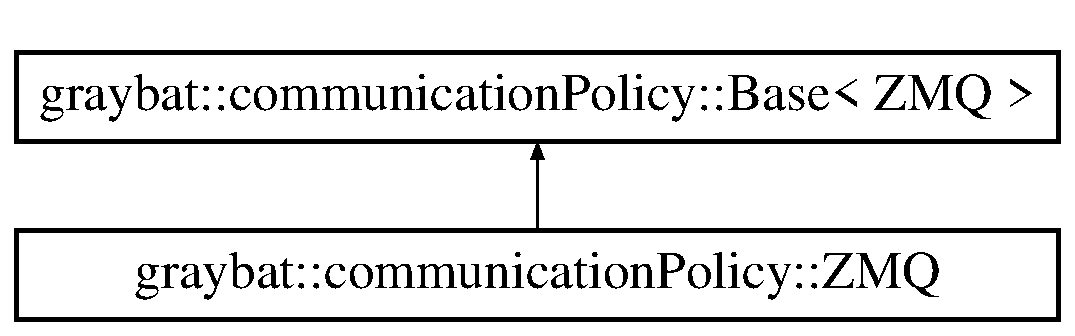
\includegraphics[height=2.000000cm]{structgraybat_1_1communicationPolicy_1_1ZMQ}
\end{center}
\end{figure}
\subsection*{Public Types}
\begin{DoxyCompactItemize}
\item 
\hypertarget{structgraybat_1_1communicationPolicy_1_1ZMQ_a70c989500cb46ab5b71768fae699759f}{}using {\bfseries Tag} = typename graybat\+::communication\+Policy\+::\+Tag$<$ \hyperlink{structgraybat_1_1communicationPolicy_1_1ZMQ}{Z\+M\+Q} $>$\label{structgraybat_1_1communicationPolicy_1_1ZMQ_a70c989500cb46ab5b71768fae699759f}

\item 
\hypertarget{structgraybat_1_1communicationPolicy_1_1ZMQ_af14a2e927b90f85e30e2eafe2fb86347}{}using {\bfseries Context\+I\+D} = typename graybat\+::communication\+Policy\+::\+Context\+I\+D$<$ \hyperlink{structgraybat_1_1communicationPolicy_1_1ZMQ}{Z\+M\+Q} $>$\label{structgraybat_1_1communicationPolicy_1_1ZMQ_af14a2e927b90f85e30e2eafe2fb86347}

\item 
\hypertarget{structgraybat_1_1communicationPolicy_1_1ZMQ_ac227f7b180d8eaee5d493b09917e10e7}{}using {\bfseries Msg\+Type} = typename graybat\+::communication\+Policy\+::\+Msg\+Type$<$ \hyperlink{structgraybat_1_1communicationPolicy_1_1ZMQ}{Z\+M\+Q} $>$\label{structgraybat_1_1communicationPolicy_1_1ZMQ_ac227f7b180d8eaee5d493b09917e10e7}

\item 
\hypertarget{structgraybat_1_1communicationPolicy_1_1ZMQ_a073da259521988b9e3ecacfc8db18029}{}using {\bfseries Msg\+I\+D} = typename graybat\+::communication\+Policy\+::\+Msg\+I\+D$<$ \hyperlink{structgraybat_1_1communicationPolicy_1_1ZMQ}{Z\+M\+Q} $>$\label{structgraybat_1_1communicationPolicy_1_1ZMQ_a073da259521988b9e3ecacfc8db18029}

\item 
\hypertarget{structgraybat_1_1communicationPolicy_1_1ZMQ_a6a60449eee02f72a8b6998dcd8eacb83}{}using {\bfseries V\+Addr} = typename graybat\+::communication\+Policy\+::\+V\+Addr$<$ \hyperlink{structgraybat_1_1communicationPolicy_1_1ZMQ}{Z\+M\+Q} $>$\label{structgraybat_1_1communicationPolicy_1_1ZMQ_a6a60449eee02f72a8b6998dcd8eacb83}

\item 
\hypertarget{structgraybat_1_1communicationPolicy_1_1ZMQ_a1675812d40f395451e11cabfd5fb28e1}{}using {\bfseries Context} = typename graybat\+::communication\+Policy\+::\+Context$<$ \hyperlink{structgraybat_1_1communicationPolicy_1_1ZMQ}{Z\+M\+Q} $>$\label{structgraybat_1_1communicationPolicy_1_1ZMQ_a1675812d40f395451e11cabfd5fb28e1}

\item 
\hypertarget{structgraybat_1_1communicationPolicy_1_1ZMQ_aa07df86b7967eeb6e35181995da85b4e}{}using {\bfseries Event} = typename graybat\+::communication\+Policy\+::\+Event$<$ \hyperlink{structgraybat_1_1communicationPolicy_1_1ZMQ}{Z\+M\+Q} $>$\label{structgraybat_1_1communicationPolicy_1_1ZMQ_aa07df86b7967eeb6e35181995da85b4e}

\item 
\hypertarget{structgraybat_1_1communicationPolicy_1_1ZMQ_a4b303911562bc088c3f85695a473e538}{}using {\bfseries Config} = typename graybat\+::communication\+Policy\+::\+Config$<$ \hyperlink{structgraybat_1_1communicationPolicy_1_1ZMQ}{Z\+M\+Q} $>$\label{structgraybat_1_1communicationPolicy_1_1ZMQ_a4b303911562bc088c3f85695a473e538}

\item 
\hypertarget{structgraybat_1_1communicationPolicy_1_1ZMQ_a1d25a8ae54bc4e64a65bff42470ca286}{}using {\bfseries Uri} = std\+::string\label{structgraybat_1_1communicationPolicy_1_1ZMQ_a1d25a8ae54bc4e64a65bff42470ca286}

\end{DoxyCompactItemize}
\subsection*{Public Member Functions}
\begin{DoxyCompactItemize}
\item 
\hypertarget{structgraybat_1_1communicationPolicy_1_1ZMQ_a1a8194fd0d25a4bd68f6eb01580ecaf0}{}{\bfseries Z\+M\+Q} (Config const config)\label{structgraybat_1_1communicationPolicy_1_1ZMQ_a1a8194fd0d25a4bd68f6eb01580ecaf0}

\item 
\hypertarget{structgraybat_1_1communicationPolicy_1_1ZMQ_a3e2677f395338d07c90b55afd66d9974}{}{\bfseries Z\+M\+Q} (\hyperlink{structgraybat_1_1communicationPolicy_1_1ZMQ}{Z\+M\+Q} \&\&other)=delete\label{structgraybat_1_1communicationPolicy_1_1ZMQ_a3e2677f395338d07c90b55afd66d9974}

\item 
\hypertarget{structgraybat_1_1communicationPolicy_1_1ZMQ_a5efe1d58e60411ea1f311b1b4eb61593}{}{\bfseries Z\+M\+Q} (\hyperlink{structgraybat_1_1communicationPolicy_1_1ZMQ}{Z\+M\+Q} \&other)=delete\label{structgraybat_1_1communicationPolicy_1_1ZMQ_a5efe1d58e60411ea1f311b1b4eb61593}

\end{DoxyCompactItemize}
\begin{Indent}{\bf Point to Point Communication Interface}\par
\begin{DoxyCompactItemize}
\item 
{\footnotesize template$<$typename T\+\_\+\+Send $>$ }\\void \hyperlink{structgraybat_1_1communicationPolicy_1_1ZMQ_a0b0b0a5a6f6b5c85a6c5b5b31fae6b1f}{send} (const V\+Addr dest\+V\+Addr, const \hyperlink{structTag}{Tag} tag, const Context context, const T\+\_\+\+Send \&send\+Data)
\begin{DoxyCompactList}\small\item\em Blocking transmission of a message send\+Data to peer with virtual address dest\+V\+Addr. \end{DoxyCompactList}\item 
{\footnotesize template$<$typename T\+\_\+\+Send $>$ }\\Event \hyperlink{structgraybat_1_1communicationPolicy_1_1ZMQ_a90e4cec7521e061aa682559d8bc72f1b}{async\+Send} (const V\+Addr dest\+V\+Addr, const \hyperlink{structTag}{Tag} tag, const Context context, T\+\_\+\+Send \&send\+Data)
\begin{DoxyCompactList}\small\item\em Non blocking transmission of a message send\+Data to peer with virtual address dest\+V\+Addr. \end{DoxyCompactList}\item 
\hypertarget{structgraybat_1_1communicationPolicy_1_1ZMQ_aba035ac9e25e20c89581c2e9ebdcf477}{}{\footnotesize template$<$typename T\+\_\+\+Send $>$ }\\void {\bfseries async\+Send\+Impl} (const Msg\+Type msg\+Type, const Msg\+I\+D msg\+I\+D, const Context context, const V\+Addr dest\+V\+Addr, const \hyperlink{structTag}{Tag} tag, T\+\_\+\+Send \&send\+Data)\label{structgraybat_1_1communicationPolicy_1_1ZMQ_aba035ac9e25e20c89581c2e9ebdcf477}

\item 
{\footnotesize template$<$typename T\+\_\+\+Recv $>$ }\\void \hyperlink{structgraybat_1_1communicationPolicy_1_1ZMQ_aed8fd6ad0f54a44d576f71e812064b17}{recv} (const V\+Addr src\+V\+Addr, const \hyperlink{structTag}{Tag} tag, const Context context, T\+\_\+\+Recv \&recv\+Data)
\begin{DoxyCompactList}\small\item\em Blocking receive of a message recv\+Data from peer with virtual address src\+V\+Addr. \end{DoxyCompactList}\item 
\hypertarget{structgraybat_1_1communicationPolicy_1_1ZMQ_a90e24f2d8431d0289d2067ed6a02f64c}{}{\footnotesize template$<$typename T\+\_\+\+Recv $>$ }\\Event {\bfseries recv} (const Context context, T\+\_\+\+Recv \&recv\+Data)\label{structgraybat_1_1communicationPolicy_1_1ZMQ_a90e24f2d8431d0289d2067ed6a02f64c}

\item 
\hypertarget{structgraybat_1_1communicationPolicy_1_1ZMQ_aca65dd2ffd1049f72e194c13968b846c}{}{\footnotesize template$<$typename T\+\_\+\+Recv $>$ }\\void {\bfseries recv\+Impl} (const Msg\+Type msg\+Type, const Context context, const V\+Addr src\+V\+Addr, const \hyperlink{structTag}{Tag} tag, T\+\_\+\+Recv \&recv\+Data)\label{structgraybat_1_1communicationPolicy_1_1ZMQ_aca65dd2ffd1049f72e194c13968b846c}

\item 
\hypertarget{structgraybat_1_1communicationPolicy_1_1ZMQ_a0c112e35dba53faa1ee222dc722eb20e}{}{\footnotesize template$<$typename T\+\_\+\+Recv $>$ }\\Event {\bfseries recv\+Impl} (const Context context, T\+\_\+\+Recv \&recv\+Data)\label{structgraybat_1_1communicationPolicy_1_1ZMQ_a0c112e35dba53faa1ee222dc722eb20e}

\item 
\hypertarget{structgraybat_1_1communicationPolicy_1_1ZMQ_aff4a73567456ebb5bf0a2a17bd8170fc}{}void {\bfseries wait} (const Msg\+Type msg\+I\+D, const Context context, const V\+Addr v\+Addr, const \hyperlink{structTag}{Tag} tag)\label{structgraybat_1_1communicationPolicy_1_1ZMQ_aff4a73567456ebb5bf0a2a17bd8170fc}

\item 
\hypertarget{structgraybat_1_1communicationPolicy_1_1ZMQ_acc3da7a5e16668628ae74161f6ab8e7b}{}bool {\bfseries ready} (const Msg\+Type msg\+I\+D, const Context context, const V\+Addr v\+Addr, const \hyperlink{structTag}{Tag} tag)\label{structgraybat_1_1communicationPolicy_1_1ZMQ_acc3da7a5e16668628ae74161f6ab8e7b}

\end{DoxyCompactItemize}
\end{Indent}
\begin{Indent}{\bf Context Interface}\par
\begin{DoxyCompactItemize}
\item 
Context \hyperlink{structgraybat_1_1communicationPolicy_1_1ZMQ_a6760648ce6f21fefad245292c46565f4}{split\+Context} (const bool is\+Member, const Context old\+Context)
\item 
\hypertarget{structgraybat_1_1communicationPolicy_1_1ZMQ_a8146abbd757a057ad24a929667a01ee6}{}Context \hyperlink{structgraybat_1_1communicationPolicy_1_1ZMQ_a8146abbd757a057ad24a929667a01ee6}{get\+Global\+Context} ()\label{structgraybat_1_1communicationPolicy_1_1ZMQ_a8146abbd757a057ad24a929667a01ee6}

\begin{DoxyCompactList}\small\item\em Returns the context that contains all peers. \end{DoxyCompactList}\end{DoxyCompactItemize}
\end{Indent}
\subsection*{Public Attributes}
\begin{DoxyCompactItemize}
\item 
\hypertarget{structgraybat_1_1communicationPolicy_1_1ZMQ_ac28925f4c8d0617d97283c18ed164217}{}\+::zmq\+::context\+\_\+t {\bfseries zmq\+Context}\label{structgraybat_1_1communicationPolicy_1_1ZMQ_ac28925f4c8d0617d97283c18ed164217}

\item 
\hypertarget{structgraybat_1_1communicationPolicy_1_1ZMQ_a7f9215005287fcb30fb21d21b10405fb}{}\+::zmq\+::context\+\_\+t {\bfseries zmq\+Signaling\+Context}\label{structgraybat_1_1communicationPolicy_1_1ZMQ_a7f9215005287fcb30fb21d21b10405fb}

\item 
\hypertarget{structgraybat_1_1communicationPolicy_1_1ZMQ_a55d3e9da96fd2deeada98ee678860cf9}{}\+::zmq\+::socket\+\_\+t {\bfseries recv\+Socket}\label{structgraybat_1_1communicationPolicy_1_1ZMQ_a55d3e9da96fd2deeada98ee678860cf9}

\item 
\hypertarget{structgraybat_1_1communicationPolicy_1_1ZMQ_ad3d52816f168d192b556ac1dc3d1e885}{}\+::zmq\+::socket\+\_\+t {\bfseries signaling\+Socket}\label{structgraybat_1_1communicationPolicy_1_1ZMQ_ad3d52816f168d192b556ac1dc3d1e885}

\item 
\hypertarget{structgraybat_1_1communicationPolicy_1_1ZMQ_a9d39af0540599d02ca1fbe3c3a3c53c6}{}const int {\bfseries zmq\+Hwm}\label{structgraybat_1_1communicationPolicy_1_1ZMQ_a9d39af0540599d02ca1fbe3c3a3c53c6}

\item 
\hypertarget{structgraybat_1_1communicationPolicy_1_1ZMQ_ac3194b52e98b31ada473e873f631b907}{}Context {\bfseries initial\+Context}\label{structgraybat_1_1communicationPolicy_1_1ZMQ_ac3194b52e98b31ada473e873f631b907}

\item 
\hypertarget{structgraybat_1_1communicationPolicy_1_1ZMQ_aaa8ad1285b17daba34d283a34349e3bc}{}std\+::map$<$ Context\+I\+D, std\+::map$<$ V\+Addr, std\+::size\+\_\+t $>$ $>$ {\bfseries send\+Socket\+Mappings}\label{structgraybat_1_1communicationPolicy_1_1ZMQ_aaa8ad1285b17daba34d283a34349e3bc}

\item 
\hypertarget{structgraybat_1_1communicationPolicy_1_1ZMQ_a6bd8f4319623f0a5ff4954fed2802009}{}std\+::vector$<$\+::zmq\+::socket\+\_\+t $>$ {\bfseries send\+Sockets}\label{structgraybat_1_1communicationPolicy_1_1ZMQ_a6bd8f4319623f0a5ff4954fed2802009}

\item 
\hypertarget{structgraybat_1_1communicationPolicy_1_1ZMQ_aacf828766b08157f9e13172949bc447b}{}std\+::map$<$ Context\+I\+D, std\+::map$<$ V\+Addr, Uri $>$ $>$ {\bfseries phone\+Book}\label{structgraybat_1_1communicationPolicy_1_1ZMQ_aacf828766b08157f9e13172949bc447b}

\item 
\hypertarget{structgraybat_1_1communicationPolicy_1_1ZMQ_a3c28dcbf8c7e5af3b282a3116130ade0}{}std\+::map$<$ Context\+I\+D, std\+::map$<$ Uri, V\+Addr $>$ $>$ {\bfseries inverse\+Phone\+Book}\label{structgraybat_1_1communicationPolicy_1_1ZMQ_a3c28dcbf8c7e5af3b282a3116130ade0}

\item 
\hypertarget{structgraybat_1_1communicationPolicy_1_1ZMQ_ab24f971152ddf296cf9e37a84f72ba43}{}std\+::map$<$ Context\+I\+D, Context $>$ {\bfseries contexts}\label{structgraybat_1_1communicationPolicy_1_1ZMQ_ab24f971152ddf296cf9e37a84f72ba43}

\item 
\hypertarget{structgraybat_1_1communicationPolicy_1_1ZMQ_a048cd99c3b30b8269695800aeec8b6b5}{}utils\+::\+Message\+Box$<$\+::zmq\+::message\+\_\+t, Msg\+Type, Context\+I\+D, V\+Addr, \hyperlink{structTag}{Tag} $>$ {\bfseries in\+Box}\label{structgraybat_1_1communicationPolicy_1_1ZMQ_a048cd99c3b30b8269695800aeec8b6b5}

\item 
\hypertarget{structgraybat_1_1communicationPolicy_1_1ZMQ_a5d8937267cb65df0d1954304eb60c060}{}unsigned {\bfseries max\+Msg\+I\+D}\label{structgraybat_1_1communicationPolicy_1_1ZMQ_a5d8937267cb65df0d1954304eb60c060}

\item 
\hypertarget{structgraybat_1_1communicationPolicy_1_1ZMQ_a0a46bd55b77c5d1638ee45779f591251}{}std\+::thread {\bfseries recv\+Handler}\label{structgraybat_1_1communicationPolicy_1_1ZMQ_a0a46bd55b77c5d1638ee45779f591251}

\item 
\hypertarget{structgraybat_1_1communicationPolicy_1_1ZMQ_a6330356fc4e18a28f820ad0d1ffd9b6c}{}std\+::mutex {\bfseries send\+Mtx}\label{structgraybat_1_1communicationPolicy_1_1ZMQ_a6330356fc4e18a28f820ad0d1ffd9b6c}

\item 
\hypertarget{structgraybat_1_1communicationPolicy_1_1ZMQ_ae962deaa23647ec055cdcb7ca91c5da6}{}std\+::mutex {\bfseries recv\+Mtx}\label{structgraybat_1_1communicationPolicy_1_1ZMQ_ae962deaa23647ec055cdcb7ca91c5da6}

\item 
\hypertarget{structgraybat_1_1communicationPolicy_1_1ZMQ_aeeeee6bb1e189218a66f53d442cc0726}{}const Uri {\bfseries master\+Uri}\label{structgraybat_1_1communicationPolicy_1_1ZMQ_aeeeee6bb1e189218a66f53d442cc0726}

\item 
\hypertarget{structgraybat_1_1communicationPolicy_1_1ZMQ_a0f4be8b5db76294a90adc532672f86a8}{}const Uri {\bfseries peer\+Uri}\label{structgraybat_1_1communicationPolicy_1_1ZMQ_a0f4be8b5db76294a90adc532672f86a8}

\end{DoxyCompactItemize}
\subsection*{Static Public Attributes}
\begin{DoxyCompactItemize}
\item 
\hypertarget{structgraybat_1_1communicationPolicy_1_1ZMQ_a75693f5486b00722fde46828a370a3e1}{}static const Msg\+Type {\bfseries V\+A\+D\+D\+R\+\_\+\+R\+E\+Q\+U\+E\+S\+T} = 0\label{structgraybat_1_1communicationPolicy_1_1ZMQ_a75693f5486b00722fde46828a370a3e1}

\item 
\hypertarget{structgraybat_1_1communicationPolicy_1_1ZMQ_ac9a6d846b671d488ccc2b48a213cb65c}{}static const Msg\+Type {\bfseries V\+A\+D\+D\+R\+\_\+\+L\+O\+O\+K\+U\+P} = 1\label{structgraybat_1_1communicationPolicy_1_1ZMQ_ac9a6d846b671d488ccc2b48a213cb65c}

\item 
\hypertarget{structgraybat_1_1communicationPolicy_1_1ZMQ_aa5fff922697df13ba51ab9c211125561}{}static const Msg\+Type {\bfseries D\+E\+S\+T\+R\+U\+C\+T} = 2\label{structgraybat_1_1communicationPolicy_1_1ZMQ_aa5fff922697df13ba51ab9c211125561}

\item 
\hypertarget{structgraybat_1_1communicationPolicy_1_1ZMQ_a3ebabd8f81881cd6ca82083da5912dc0}{}static const Msg\+Type {\bfseries R\+E\+T\+R\+Y} = 3\label{structgraybat_1_1communicationPolicy_1_1ZMQ_a3ebabd8f81881cd6ca82083da5912dc0}

\item 
\hypertarget{structgraybat_1_1communicationPolicy_1_1ZMQ_ae738003867ad7590787fbd72e470a0c7}{}static const Msg\+Type {\bfseries A\+C\+K} = 4\label{structgraybat_1_1communicationPolicy_1_1ZMQ_ae738003867ad7590787fbd72e470a0c7}

\item 
\hypertarget{structgraybat_1_1communicationPolicy_1_1ZMQ_a0fa73b38f80d3d2d2761b014ffd64410}{}static const Msg\+Type {\bfseries C\+O\+N\+T\+E\+X\+T\+\_\+\+I\+N\+I\+T} = 5\label{structgraybat_1_1communicationPolicy_1_1ZMQ_a0fa73b38f80d3d2d2761b014ffd64410}

\item 
\hypertarget{structgraybat_1_1communicationPolicy_1_1ZMQ_a36274d861cda1c40bf2cd384f359ac36}{}static const Msg\+Type {\bfseries C\+O\+N\+T\+E\+X\+T\+\_\+\+R\+E\+Q\+U\+E\+S\+T} = 6\label{structgraybat_1_1communicationPolicy_1_1ZMQ_a36274d861cda1c40bf2cd384f359ac36}

\item 
\hypertarget{structgraybat_1_1communicationPolicy_1_1ZMQ_a838f1280768e4b09b0f67cf202c4693f}{}static const Msg\+Type {\bfseries P\+E\+E\+R} = 7\label{structgraybat_1_1communicationPolicy_1_1ZMQ_a838f1280768e4b09b0f67cf202c4693f}

\item 
\hypertarget{structgraybat_1_1communicationPolicy_1_1ZMQ_a080083ad95e8edd5005dfa87dc247c9e}{}static const Msg\+Type {\bfseries C\+O\+N\+F\+I\+R\+M} = 8\label{structgraybat_1_1communicationPolicy_1_1ZMQ_a080083ad95e8edd5005dfa87dc247c9e}

\item 
\hypertarget{structgraybat_1_1communicationPolicy_1_1ZMQ_a253f8c42a3b412656465686ac4302556}{}static const Msg\+Type {\bfseries S\+P\+L\+I\+T} = 9\label{structgraybat_1_1communicationPolicy_1_1ZMQ_a253f8c42a3b412656465686ac4302556}

\end{DoxyCompactItemize}
\subsection*{Z\+M\+Q Utility functions}
\begin{DoxyCompactItemize}
\item 
\hypertarget{structgraybat_1_1communicationPolicy_1_1ZMQ_acabe8e002759a5893d7f2e935dae401e}{}Context\+I\+D {\bfseries get\+Initial\+Context\+I\+D} (\+::zmq\+::socket\+\_\+t \&socket, const size\+\_\+t context\+Size)\label{structgraybat_1_1communicationPolicy_1_1ZMQ_acabe8e002759a5893d7f2e935dae401e}

\item 
\hypertarget{structgraybat_1_1communicationPolicy_1_1ZMQ_a40180b6802337e67d2b5e3b981caad38}{}Context\+I\+D {\bfseries get\+Context\+I\+D} (\+::zmq\+::socket\+\_\+t \&socket)\label{structgraybat_1_1communicationPolicy_1_1ZMQ_a40180b6802337e67d2b5e3b981caad38}

\item 
\hypertarget{structgraybat_1_1communicationPolicy_1_1ZMQ_a037bd2bd2fc50566f6f3934f620fd8f2}{}V\+Addr {\bfseries get\+V\+Addr} (\+::zmq\+::socket\+\_\+t \&socket, const Context\+I\+D context\+I\+D, const Uri uri)\label{structgraybat_1_1communicationPolicy_1_1ZMQ_a037bd2bd2fc50566f6f3934f620fd8f2}

\item 
\hypertarget{structgraybat_1_1communicationPolicy_1_1ZMQ_a7c902560de928d4e60a7e750afe252b6}{}Uri {\bfseries get\+Uri} (\+::zmq\+::socket\+\_\+t \&socket, const Context\+I\+D context\+I\+D, const V\+Addr v\+Addr)\label{structgraybat_1_1communicationPolicy_1_1ZMQ_a7c902560de928d4e60a7e750afe252b6}

\item 
\hypertarget{structgraybat_1_1communicationPolicy_1_1ZMQ_ac758b90217607dbd584f0fa8c275b5ab}{}Msg\+I\+D {\bfseries get\+Msg\+I\+D} ()\label{structgraybat_1_1communicationPolicy_1_1ZMQ_ac758b90217607dbd584f0fa8c275b5ab}

\item 
\hypertarget{structgraybat_1_1communicationPolicy_1_1ZMQ_ae2a07880da111ca0f60f4fd811b36a63}{}{\footnotesize template$<$typename T\+\_\+\+Data $>$ }\\void {\bfseries zmq\+Message\+To\+Data} (\+::zmq\+::message\+\_\+t \&message, T\+\_\+\+Data \&data)\label{structgraybat_1_1communicationPolicy_1_1ZMQ_ae2a07880da111ca0f60f4fd811b36a63}

\item 
\hypertarget{structgraybat_1_1communicationPolicy_1_1ZMQ_a4b944514212a53c7bd653370a5e5523a}{}Uri {\bfseries bind\+To\+Next\+Free\+Port} (\+::zmq\+::socket\+\_\+t \&socket, const std\+::string peer\+Uri)\label{structgraybat_1_1communicationPolicy_1_1ZMQ_a4b944514212a53c7bd653370a5e5523a}

\item 
\hypertarget{structgraybat_1_1communicationPolicy_1_1ZMQ_a252494da3e7481ba0858b8989ff3885b}{}void {\bfseries handle\+Recv} ()\label{structgraybat_1_1communicationPolicy_1_1ZMQ_a252494da3e7481ba0858b8989ff3885b}

\item 
\hypertarget{structgraybat_1_1communicationPolicy_1_1ZMQ_ae539febea7852f497dc3e5b45210d8da}{}static char $\ast$ {\bfseries s\+\_\+recv} (\+::zmq\+::socket\+\_\+t \&socket)\label{structgraybat_1_1communicationPolicy_1_1ZMQ_ae539febea7852f497dc3e5b45210d8da}

\item 
\hypertarget{structgraybat_1_1communicationPolicy_1_1ZMQ_a61f299de4f180b2981ad1427f7a120fd}{}static int {\bfseries s\+\_\+send} (\+::zmq\+::socket\+\_\+t \&socket, const char $\ast$string)\label{structgraybat_1_1communicationPolicy_1_1ZMQ_a61f299de4f180b2981ad1427f7a120fd}

\end{DoxyCompactItemize}


\subsection{Detailed Description}
Implementation of the \hyperlink{structgraybat_1_1Cage}{Cage} communication\+Policy interface based on \hyperlink{structgraybat_1_1communicationPolicy_1_1ZMQ}{Z\+M\+Q}. 

\subsection{Member Function Documentation}
\hypertarget{structgraybat_1_1communicationPolicy_1_1ZMQ_a90e4cec7521e061aa682559d8bc72f1b}{}\index{graybat\+::communication\+Policy\+::\+Z\+M\+Q@{graybat\+::communication\+Policy\+::\+Z\+M\+Q}!async\+Send@{async\+Send}}
\index{async\+Send@{async\+Send}!graybat\+::communication\+Policy\+::\+Z\+M\+Q@{graybat\+::communication\+Policy\+::\+Z\+M\+Q}}
\subsubsection[{async\+Send(const V\+Addr dest\+V\+Addr, const Tag tag, const Context context, T\+\_\+\+Send \&send\+Data)}]{\setlength{\rightskip}{0pt plus 5cm}template$<$typename T\+\_\+\+Send $>$ Event graybat\+::communication\+Policy\+::\+Z\+M\+Q\+::async\+Send (
\begin{DoxyParamCaption}
\item[{const V\+Addr}]{dest\+V\+Addr, }
\item[{const {\bf Tag}}]{tag, }
\item[{const Context}]{context, }
\item[{T\+\_\+\+Send \&}]{send\+Data}
\end{DoxyParamCaption}
)\hspace{0.3cm}{\ttfamily [inline]}}\label{structgraybat_1_1communicationPolicy_1_1ZMQ_a90e4cec7521e061aa682559d8bc72f1b}


Non blocking transmission of a message send\+Data to peer with virtual address dest\+V\+Addr. 


\begin{DoxyParams}[1]{Parameters}
\mbox{\tt in}  & {\em dest\+V\+Addr} & V\+Addr of peer that will receive the message \\
\hline
\mbox{\tt in}  & {\em tag} & Description of the message to better distinguish messages types \\
\hline
\mbox{\tt in}  & {\em context} & Context in which both sender and receiver are included \\
\hline
\mbox{\tt in}  & {\em send\+Data} & Data reference of template type T will be. T need to provide the function data(), that returns the pointer to the data memory address. And the function size(), that return the amount of data elements to send. Notice, that std\+::vector and std\+::array implement this interface.\\
\hline
\end{DoxyParams}
\begin{DoxyReturn}{Returns}
Event 
\end{DoxyReturn}
\hypertarget{structgraybat_1_1communicationPolicy_1_1ZMQ_aed8fd6ad0f54a44d576f71e812064b17}{}\index{graybat\+::communication\+Policy\+::\+Z\+M\+Q@{graybat\+::communication\+Policy\+::\+Z\+M\+Q}!recv@{recv}}
\index{recv@{recv}!graybat\+::communication\+Policy\+::\+Z\+M\+Q@{graybat\+::communication\+Policy\+::\+Z\+M\+Q}}
\subsubsection[{recv(const V\+Addr src\+V\+Addr, const Tag tag, const Context context, T\+\_\+\+Recv \&recv\+Data)}]{\setlength{\rightskip}{0pt plus 5cm}template$<$typename T\+\_\+\+Recv $>$ void graybat\+::communication\+Policy\+::\+Z\+M\+Q\+::recv (
\begin{DoxyParamCaption}
\item[{const V\+Addr}]{src\+V\+Addr, }
\item[{const {\bf Tag}}]{tag, }
\item[{const Context}]{context, }
\item[{T\+\_\+\+Recv \&}]{recv\+Data}
\end{DoxyParamCaption}
)\hspace{0.3cm}{\ttfamily [inline]}}\label{structgraybat_1_1communicationPolicy_1_1ZMQ_aed8fd6ad0f54a44d576f71e812064b17}


Blocking receive of a message recv\+Data from peer with virtual address src\+V\+Addr. 


\begin{DoxyParams}[1]{Parameters}
\mbox{\tt in}  & {\em src\+V\+Addr} & V\+Addr of peer that sended the message \\
\hline
\mbox{\tt in}  & {\em tag} & Description of the message to better distinguish messages types \\
\hline
\mbox{\tt in}  & {\em context} & Context in which both sender and receiver are included \\
\hline
\mbox{\tt out}  & {\em recv\+Data} & Data reference of template type T will be received from sender peer. T need to provide the function data(), that returns the pointer to the data memory address. And the function size(), that return the amount of data elements to send. Notice, that std\+::vector and std\+::array implement this interface. \\
\hline
\end{DoxyParams}
\hypertarget{structgraybat_1_1communicationPolicy_1_1ZMQ_a0b0b0a5a6f6b5c85a6c5b5b31fae6b1f}{}\index{graybat\+::communication\+Policy\+::\+Z\+M\+Q@{graybat\+::communication\+Policy\+::\+Z\+M\+Q}!send@{send}}
\index{send@{send}!graybat\+::communication\+Policy\+::\+Z\+M\+Q@{graybat\+::communication\+Policy\+::\+Z\+M\+Q}}
\subsubsection[{send(const V\+Addr dest\+V\+Addr, const Tag tag, const Context context, const T\+\_\+\+Send \&send\+Data)}]{\setlength{\rightskip}{0pt plus 5cm}template$<$typename T\+\_\+\+Send $>$ void graybat\+::communication\+Policy\+::\+Z\+M\+Q\+::send (
\begin{DoxyParamCaption}
\item[{const V\+Addr}]{dest\+V\+Addr, }
\item[{const {\bf Tag}}]{tag, }
\item[{const Context}]{context, }
\item[{const T\+\_\+\+Send \&}]{send\+Data}
\end{DoxyParamCaption}
)\hspace{0.3cm}{\ttfamily [inline]}}\label{structgraybat_1_1communicationPolicy_1_1ZMQ_a0b0b0a5a6f6b5c85a6c5b5b31fae6b1f}


Blocking transmission of a message send\+Data to peer with virtual address dest\+V\+Addr. 


\begin{DoxyParams}[1]{Parameters}
\mbox{\tt in}  & {\em dest\+V\+Addr} & V\+Addr of peer that will receive the message \\
\hline
\mbox{\tt in}  & {\em tag} & Description of the message to better distinguish messages types \\
\hline
\mbox{\tt in}  & {\em context} & Context in which both sender and receiver are included \\
\hline
\mbox{\tt in}  & {\em send\+Data} & Data reference of template type T will be send to receiver peer. T need to provide the function data(), that returns the pointer to the data memory address. And the function size(), that return the amount of data elements to send. Notice, that std\+::vector and std\+::array implement this interface. \\
\hline
\end{DoxyParams}
\hypertarget{structgraybat_1_1communicationPolicy_1_1ZMQ_a6760648ce6f21fefad245292c46565f4}{}\index{graybat\+::communication\+Policy\+::\+Z\+M\+Q@{graybat\+::communication\+Policy\+::\+Z\+M\+Q}!split\+Context@{split\+Context}}
\index{split\+Context@{split\+Context}!graybat\+::communication\+Policy\+::\+Z\+M\+Q@{graybat\+::communication\+Policy\+::\+Z\+M\+Q}}
\subsubsection[{split\+Context(const bool is\+Member, const Context old\+Context)}]{\setlength{\rightskip}{0pt plus 5cm}Context graybat\+::communication\+Policy\+::\+Z\+M\+Q\+::split\+Context (
\begin{DoxyParamCaption}
\item[{const bool}]{is\+Member, }
\item[{const Context}]{old\+Context}
\end{DoxyParamCaption}
)\hspace{0.3cm}{\ttfamily [inline]}}\label{structgraybat_1_1communicationPolicy_1_1ZMQ_a6760648ce6f21fefad245292c46565f4}


The documentation for this class was generated from the following file\+:\begin{DoxyCompactItemize}
\item 
include/graybat/communication\+Policy/Z\+M\+Q.\+hpp\end{DoxyCompactItemize}

\chapter{Example Documentation}
\hypertarget{anyrecv_8cpp-example}{}\section{anyrecv.\+cpp}
A master recv messages from all slaves and answers.


\begin{DoxyCodeInclude}

\textcolor{comment}{// STL}
\textcolor{preprocessor}{#include <iostream>}   \textcolor{comment}{/* std::cout */}
\textcolor{preprocessor}{#include <vector>}     \textcolor{comment}{/* std::vector */}
\textcolor{preprocessor}{#include <array>}      \textcolor{comment}{/* std::array */}
\textcolor{preprocessor}{#include <functional>} \textcolor{comment}{/* std::bind */}

\textcolor{comment}{// GRAYBAT}
\textcolor{preprocessor}{#include <graybat/Cage.hpp>}
\textcolor{preprocessor}{#include <graybat/communicationPolicy/BMPI.hpp>}
\textcolor{preprocessor}{#include <graybat/graphPolicy/BGL.hpp>}
\textcolor{comment}{// GRAYBAT mappings}
\textcolor{preprocessor}{#include <graybat/mapping/Consecutive.hpp>}
\textcolor{preprocessor}{#include <graybat/mapping/Random.hpp>}
\textcolor{preprocessor}{#include <graybat/mapping/Roundrobin.hpp>}
\textcolor{comment}{// GRAYBAT pattern}
\textcolor{preprocessor}{#include <graybat/pattern/GridDiagonal.hpp>}
\textcolor{preprocessor}{#include <graybat/pattern/Chain.hpp>}
\textcolor{preprocessor}{#include <graybat/pattern/BiStar.hpp>}

\textcolor{keyword}{struct }\hyperlink{structFunction}{Function} \{
    
    \textcolor{keywordtype}{void} process(std::array<unsigned, 1> &data)\{
    foo(std::get<0>(data));
    
    \}

    std::function<void (unsigned&)> foo;
\};


\textcolor{keywordtype}{int} exp() \{
    \textcolor{comment}{/***************************************************************************}
\textcolor{comment}{     * Configuration}
\textcolor{comment}{     ****************************************************************************/}

    \textcolor{comment}{// CommunicationPolicy}
    \textcolor{keyword}{typedef} \hyperlink{structgraybat_1_1communicationPolicy_1_1BMPI}{graybat::communicationPolicy::BMPI} CP;
    \textcolor{keyword}{typedef} CP::Config                         Config;    
    
    \textcolor{comment}{// GraphPolicy}
    \textcolor{keyword}{typedef} \hyperlink{classgraybat_1_1graphPolicy_1_1BGL}{graybat::graphPolicy::BGL<Function>}    GP;
    
    \textcolor{comment}{// Cage}
    \textcolor{keyword}{typedef} \hyperlink{structgraybat_1_1Cage}{graybat::Cage<CP, GP>} Cage;
    \textcolor{keyword}{typedef} \textcolor{keyword}{typename} Cage::Vertex Vertex;
    \textcolor{keyword}{typedef} \textcolor{keyword}{typename} Cage::Edge Edge;

    \textcolor{comment}{/***************************************************************************}
\textcolor{comment}{     * Initialize Communication}
\textcolor{comment}{     ****************************************************************************/}
    \textcolor{comment}{// Create GoL Graph}
    Config config;
    Cage cage(config);

    \textcolor{comment}{// Set communication pattern}
    cage.setGraph(\hyperlink{structgraybat_1_1pattern_1_1BiStar}{graybat::pattern::BiStar<GP>}(cage.getPeers().size()));

    \textcolor{comment}{// Distribute vertices}
    cage.distribute(\hyperlink{structgraybat_1_1mapping_1_1Consecutive}{graybat::mapping::Consecutive}());
        

    \textcolor{comment}{/***************************************************************************}
\textcolor{comment}{     * Run Simulation}
\textcolor{comment}{     ****************************************************************************/}
    \textcolor{comment}{//std::vector<Event> events;}

    std::array<unsigned, 1> input \{\{0\}\};
    std::array<unsigned, 1> output \{\{0\}\};

    \textcolor{keyword}{const} Vertex reply = cage.getVertex(0);
    
    \textcolor{keywordflow}{for}(Vertex v : cage.hostedVertices)\{


        \textcolor{keywordflow}{if}(v == reply)\{
            \textcolor{keywordflow}{while}(\textcolor{keyword}{true})\{
                Edge e = cage.recv(output);
                std::cout << \textcolor{stringliteral}{"Got msg from "} << e.source.id << \textcolor{stringliteral}{": "}<< output[0] << std::endl;
                output[0]++;
                cage.send(e.inverse(), output);
            \}
            
        \}
        \textcolor{keywordflow}{else} \{
            input[0] = v.id;
            v.spread(input);
            v.collect(input);
            std::cout << \textcolor{stringliteral}{" Got input from master:"} << input[0] << std::endl;
        \}
 
    
    \}

    \textcolor{keywordflow}{return} 0;

\}

\textcolor{keywordtype}{int} main()\{
    exp();
    \textcolor{keywordflow}{return} 0;
\}
\end{DoxyCodeInclude}
 
\hypertarget{chain_8cpp-example}{}\section{chain.\+cpp}
Data is send through a chain of compute nodes and every node increments the value.


\begin{DoxyCodeInclude}

\textcolor{comment}{// STL}
\textcolor{preprocessor}{#include <iostream>}   \textcolor{comment}{/* std::cout */}
\textcolor{preprocessor}{#include <vector>}     \textcolor{comment}{/* std::vector */}
\textcolor{preprocessor}{#include <array>}      \textcolor{comment}{/* std::array */}
\textcolor{preprocessor}{#include <functional>} \textcolor{comment}{/* std::bind */}
\textcolor{preprocessor}{#include <cmath>}      \textcolor{comment}{/* sqrt */}
\textcolor{preprocessor}{#include <cstdlib>}    \textcolor{comment}{/* atoi */}
\textcolor{preprocessor}{#include <numeric>}    \textcolor{comment}{/* std::accumulate */}

\textcolor{comment}{// GRAYBAT}
\textcolor{preprocessor}{#include <graybat/Cage.hpp>}
\textcolor{preprocessor}{#include <graybat/communicationPolicy/BMPI.hpp>}
\textcolor{preprocessor}{#include <graybat/graphPolicy/BGL.hpp>}
\textcolor{comment}{// GRAYBAT mappings}
\textcolor{preprocessor}{#include <graybat/mapping/Consecutive.hpp>}
\textcolor{preprocessor}{#include <graybat/mapping/Random.hpp>}
\textcolor{preprocessor}{#include <graybat/mapping/Roundrobin.hpp>}
\textcolor{preprocessor}{#include <graybat/mapping/Filter.hpp>}
\textcolor{comment}{// GRAYBAT pattern}
\textcolor{preprocessor}{#include <graybat/pattern/Chain.hpp>}


\textcolor{keyword}{struct }\hyperlink{structTag}{Tag} \{
    \textcolor{keywordtype}{int} tag;
    
\};

\textcolor{keywordtype}{int} exp() \{
    \textcolor{comment}{/***************************************************************************}
\textcolor{comment}{     * Configuration}
\textcolor{comment}{     ****************************************************************************/}

    \textcolor{comment}{// CommunicationPolicy}
    \textcolor{keyword}{typedef} \hyperlink{structgraybat_1_1communicationPolicy_1_1BMPI}{graybat::communicationPolicy::BMPI} CP;
    \textcolor{keyword}{typedef} CP::Config                         Config;    
    
    \textcolor{comment}{// GraphPolicy}
    \textcolor{keyword}{typedef} \hyperlink{classgraybat_1_1graphPolicy_1_1BGL}{graybat::graphPolicy::BGL<Tag, Tag>}    GP;
    
    \textcolor{comment}{// Cage}
    \textcolor{keyword}{typedef} \hyperlink{structgraybat_1_1Cage}{graybat::Cage<CP, GP>} Cage;
    \textcolor{keyword}{typedef} \textcolor{keyword}{typename} Cage::Event  Event;
    \textcolor{keyword}{typedef} \textcolor{keyword}{typename} Cage::Vertex Vertex;

    \textcolor{comment}{/***************************************************************************}
\textcolor{comment}{     * Initialize Communication}
\textcolor{comment}{     ****************************************************************************/}
    \textcolor{keyword}{const} \textcolor{keywordtype}{unsigned} nChainLinks = 6;
    \textcolor{keyword}{auto} inc = [](\textcolor{keywordtype}{unsigned} &a)\{a++;\};

    \textcolor{comment}{// Create GoL Graph}
    Config config;
    Cage cage(config);

    cage.setGraph(\hyperlink{structgraybat_1_1pattern_1_1Chain}{graybat::pattern::Chain<GP>}(nChainLinks));
    
    \textcolor{comment}{// Distribute vertices}
    cage.distribute(\hyperlink{structgraybat_1_1mapping_1_1Filter}{graybat::mapping::Filter}(cage.comm.getGlobalContext().getVAddr(
      ) % 3));

    \textcolor{comment}{/***************************************************************************}
\textcolor{comment}{     * Run Simulation}
\textcolor{comment}{     ****************************************************************************/}
    std::vector<Event> events;

    std::array<unsigned, 1> input \{\{0\}\};
    std::array<unsigned, 1> output \{\{0\}\};
    std::array<unsigned, 1> intermediate \{\{0\}\};

    \textcolor{keyword}{const} Vertex entry = cage.getVertex(0);
    \textcolor{keyword}{const} Vertex exit  = cage.getVertex(nChainLinks-1);


    \textcolor{keywordflow}{for}(Vertex v : cage.hostedVertices)\{

        \textcolor{keywordflow}{if}(v == entry)\{
            v.spread(input, events);
            std::cout << \textcolor{stringliteral}{"Input: "} << input[0] << \textcolor{stringliteral}{" "} << cage.comm.getGlobalContext().getVAddr() << 
      std::endl;
        \}

        \textcolor{keywordflow}{if}(v == exit)\{
            v.collect(output);
            std::cout << \textcolor{stringliteral}{"Output: "} << output[0] << \textcolor{stringliteral}{" "} << cage.comm.getGlobalContext().getVAddr() << 
      std::endl;
        \}

        \textcolor{keywordflow}{if}(v != entry and v != exit)\{
            v.collect(intermediate);
            inc(intermediate[0]);
            std::cout << \textcolor{stringliteral}{"Increment: "} << intermediate[0] << \textcolor{stringliteral}{" "} << cage.comm.getGlobalContext().getVAddr()
       << std::endl;
            v.spread(intermediate, events);
        
        \}
    
    \}

    \textcolor{keywordflow}{for}(\textcolor{keywordtype}{unsigned} i = 0; i < events.size(); ++i)\{
        events.back().wait();
        events.pop\_back();
    \}
    
    \textcolor{keywordflow}{return} 0;

\}

\textcolor{keywordtype}{int} main()\{
    exp();
    \textcolor{keywordflow}{return} 0;
\}
\end{DoxyCodeInclude}
 
\hypertarget{forward_8cpp-example}{}\section{forward.\+cpp}
Data is forwarded through a chain of compute nodes.


\begin{DoxyCodeInclude}

\textcolor{comment}{// STL}
\textcolor{preprocessor}{#include <iostream>}   \textcolor{comment}{/* std::cout */}
\textcolor{preprocessor}{#include <vector>}     \textcolor{comment}{/* std::vector */}
\textcolor{preprocessor}{#include <array>}      \textcolor{comment}{/* std::array */}
\textcolor{preprocessor}{#include <functional>} \textcolor{comment}{/* std::bind */}

\textcolor{comment}{// GRAYBAT}
\textcolor{preprocessor}{#include <graybat/Cage.hpp>}
\textcolor{preprocessor}{#include <graybat/communicationPolicy/BMPI.hpp>}
\textcolor{preprocessor}{#include <graybat/graphPolicy/BGL.hpp>}
\textcolor{comment}{// GRAYBAT mappings}
\textcolor{preprocessor}{#include <graybat/mapping/Consecutive.hpp>}
\textcolor{preprocessor}{#include <graybat/mapping/Random.hpp>}
\textcolor{preprocessor}{#include <graybat/mapping/Roundrobin.hpp>}
\textcolor{comment}{// GRAYBAT pattern}
\textcolor{preprocessor}{#include <graybat/pattern/GridDiagonal.hpp>}
\textcolor{preprocessor}{#include <graybat/pattern/Chain.hpp>}

\textcolor{keyword}{struct }\hyperlink{structFunction}{Function} \{
    
    \textcolor{keywordtype}{void} process(std::array<unsigned, 1> &data)\{
    foo(std::get<0>(data));
    
    \}

    std::function<void (unsigned&)> foo;
\};


\textcolor{keywordtype}{int} exp() \{
    \textcolor{comment}{/***************************************************************************}
\textcolor{comment}{     * Configuration}
\textcolor{comment}{     ****************************************************************************/}

    \textcolor{comment}{// CommunicationPolicy}
    \textcolor{keyword}{typedef} \hyperlink{structgraybat_1_1communicationPolicy_1_1BMPI}{graybat::communicationPolicy::BMPI} CP;
    \textcolor{keyword}{typedef} CP::Config                         Config;
    
    \textcolor{comment}{// GraphPolicy}
    \textcolor{keyword}{typedef} \hyperlink{classgraybat_1_1graphPolicy_1_1BGL}{graybat::graphPolicy::BGL<Function>}    GP;
    
    \textcolor{comment}{// Cage}
    \textcolor{keyword}{typedef} \hyperlink{structgraybat_1_1Cage}{graybat::Cage<CP, GP>} Cage;
    \textcolor{keyword}{typedef} \textcolor{keyword}{typename} Cage::Event  Event;
    \textcolor{keyword}{typedef} \textcolor{keyword}{typename} Cage::Vertex Vertex;
    \textcolor{keyword}{typedef} \textcolor{keyword}{typename} Vertex::VertexProperty VertexProperty;

    \textcolor{comment}{/***************************************************************************}
\textcolor{comment}{     * Initialize Communication}
\textcolor{comment}{nn     ****************************************************************************/}
    \textcolor{keyword}{const} \textcolor{keywordtype}{unsigned} nChainLinks = 1000;
    
    \textcolor{comment}{// Create GoL Graph}
    Config config;
    Cage cage(config);

    \textcolor{comment}{// Set communication pattern}
    cage.setGraph(\hyperlink{structgraybat_1_1pattern_1_1Chain}{graybat::pattern::Chain<GP>}(nChainLinks));

    \textcolor{comment}{// Distribute vertices}
    cage.distribute(\hyperlink{structgraybat_1_1mapping_1_1Consecutive}{graybat::mapping::Consecutive}());

    \textcolor{comment}{// Set functions of vertices}
    \textcolor{keywordflow}{for}(Vertex &v : cage.getVertices())\{
    v().foo = [v](\textcolor{keywordtype}{unsigned} &a)->\textcolor{keywordtype}{void} \{a += v.id;\};
    \}
        

    \textcolor{comment}{/***************************************************************************}
\textcolor{comment}{     * Run Simulation}
\textcolor{comment}{     ****************************************************************************/}
    std::vector<Event> events;

    std::array<unsigned, 1> input \{\{0\}\};
    std::array<unsigned, 1> output \{\{0\}\};
    std::array<unsigned, 1> intermediate \{\{0\}\};

    \textcolor{keyword}{const} Vertex entry = cage.getVertex(0);
    \textcolor{keyword}{const} Vertex exit  = cage.getVertex(nChainLinks-1);
    
    \textcolor{keyword}{using namespace }std::placeholders;
    
    \textcolor{keywordflow}{for}(Vertex v : cage.hostedVertices)\{
    \textcolor{keywordflow}{if}(v == entry)\{
        v.spread(input, events);
        std::cout << \textcolor{stringliteral}{"Input: "} << input[0] << std::endl;                
    \}

    \textcolor{keywordflow}{if}(v == exit)\{
        v.collect(output);
        std::cout << \textcolor{stringliteral}{"Output: "} << output[0] << std::endl;
    \}

    \textcolor{keywordflow}{if}(v != entry and v != exit)\{
        v.forward(intermediate, std::bind(&VertexProperty::process, v(), std::placeholders::\_1));
        std::cout << \textcolor{stringliteral}{"Intermediate: "} << intermediate[0] << std::endl;
    \}
    
    \}

    \textcolor{keywordflow}{for}(\textcolor{keywordtype}{unsigned} i = 0; i < events.size(); ++i)\{
    events.back().wait();
    events.pop\_back();
    \}
    
    \textcolor{keywordflow}{return} 0;

\}

\textcolor{keywordtype}{int} main()\{
    exp();
    \textcolor{keywordflow}{return} 0;
\}
\end{DoxyCodeInclude}
 
\hypertarget{gol_8cpp-example}{}\section{gol.\+cpp}
Simple example that shows how to instantiate and use the Cage within a game of life.


\begin{DoxyCodeInclude}

\textcolor{comment}{// STL}
\textcolor{preprocessor}{#include <iostream>}   \textcolor{comment}{/* std::cout */}
\textcolor{preprocessor}{#include <vector>}     \textcolor{comment}{/* std::vector */}
\textcolor{preprocessor}{#include <array>}      \textcolor{comment}{/* std::array */}
\textcolor{preprocessor}{#include <cmath>}      \textcolor{comment}{/* sqrt */}
\textcolor{preprocessor}{#include <cstdlib>}    \textcolor{comment}{/* atoi */}
\textcolor{preprocessor}{#include <numeric>}    \textcolor{comment}{/* std::accumulate */}

\textcolor{comment}{// GRAYBAT}
\textcolor{preprocessor}{#include <graybat/Cage.hpp>}
\textcolor{preprocessor}{#include <graybat/communicationPolicy/BMPI.hpp>}
\textcolor{preprocessor}{#include <graybat/graphPolicy/BGL.hpp>}
\textcolor{comment}{// GRAYBAT mappings}
\textcolor{preprocessor}{#include <graybat/mapping/Consecutive.hpp>}
\textcolor{preprocessor}{#include <graybat/mapping/Random.hpp>}
\textcolor{preprocessor}{#include <graybat/mapping/Roundrobin.hpp>}
\textcolor{comment}{// GRAYBAT patterns}
\textcolor{preprocessor}{#include <graybat/pattern/GridDiagonal.hpp>}

\textcolor{keyword}{struct }\hyperlink{structCell}{Cell} \{
    \hyperlink{structCell}{Cell}() : isAlive\{\{0\}\}, aliveNeighbors(0)\{
    \textcolor{keywordtype}{unsigned} random = rand() % 10000;
    \textcolor{keywordflow}{if}(random < 3125)\{
        isAlive[0] = 1;
    \}

    \}
    
    std::array<unsigned, 1> isAlive;
    \textcolor{keywordtype}{unsigned} aliveNeighbors;

\};


\textcolor{keywordtype}{void} printGolDomain(\textcolor{keyword}{const} std::vector<unsigned> domain, \textcolor{keyword}{const} \textcolor{keywordtype}{unsigned} width, \textcolor{keyword}{const} \textcolor{keywordtype}{unsigned} height, \textcolor{keyword}{const} \textcolor{keywordtype}{
      unsigned} generation)\{
    \textcolor{keywordflow}{for}(\textcolor{keywordtype}{unsigned} i = 0; i < domain.size(); ++i)\{
    \textcolor{keywordflow}{if}((i % (width)) == 0)\{
        std::cerr << std::endl;
    \}

    \textcolor{keywordflow}{if}(domain.at(i))\{
        std::cerr << \textcolor{stringliteral}{"#"};
    \}
    \textcolor{keywordflow}{else} \{
        std::cerr << \textcolor{stringliteral}{" "};
    \}


    \}
    std::cerr << \textcolor{stringliteral}{"Generation: "} << generation << std::endl;
    \textcolor{keywordflow}{for}(\textcolor{keywordtype}{unsigned} i = 0; i < height+1; ++i)\{
    std::cerr << \textcolor{stringliteral}{"\(\backslash\)033[F"};
    \}

\}

\textcolor{keyword}{template} <\textcolor{keyword}{class} T\_Cell>
\textcolor{keywordtype}{void} updateState(T\_Cell &cell)\{

    \textcolor{keywordflow}{switch}(cell().aliveNeighbors)\{

    \textcolor{keywordflow}{case} 0:
    \textcolor{keywordflow}{case} 1:
    cell().isAlive[0] = 0;
    \textcolor{keywordflow}{break};

    \textcolor{keywordflow}{case} 2:
    cell().isAlive[0] = cell().isAlive[0];
    \textcolor{keywordflow}{break};
        
    \textcolor{keywordflow}{case} 3: 
    cell().isAlive[0] = 1;
    \textcolor{keywordflow}{break}; 

    \textcolor{keywordflow}{default}: 
    cell().isAlive[0] = 0;
    \textcolor{keywordflow}{break};

    \};

\}

std::array<unsigned,1> one\{\{1\}\};

\textcolor{keywordtype}{int} gol(\textcolor{keyword}{const} \textcolor{keywordtype}{unsigned} nCells, \textcolor{keyword}{const} \textcolor{keywordtype}{unsigned} nTimeSteps ) \{
    \textcolor{comment}{/***************************************************************************}
\textcolor{comment}{     * Configuration}
\textcolor{comment}{     ****************************************************************************/}

    \textcolor{comment}{// CommunicationPolicy}
    \textcolor{keyword}{typedef} \hyperlink{structgraybat_1_1communicationPolicy_1_1BMPI}{graybat::communicationPolicy::BMPI} CP;
    
    \textcolor{comment}{// GraphPolicy}
    \textcolor{keyword}{typedef} \hyperlink{classgraybat_1_1graphPolicy_1_1BGL}{graybat::graphPolicy::BGL<Cell>}    GP;
    
    \textcolor{comment}{// Cage}
    \textcolor{keyword}{typedef} \hyperlink{structgraybat_1_1Cage}{graybat::Cage<CP, GP>} Cage;
    \textcolor{keyword}{typedef} \textcolor{keyword}{typename} Cage::Event  Event;
    \textcolor{keyword}{typedef} \textcolor{keyword}{typename} Cage::Vertex Vertex;

    \textcolor{comment}{/***************************************************************************}
\textcolor{comment}{     * Initialize Communication}
\textcolor{comment}{     ****************************************************************************/}
    \textcolor{comment}{// Set Graph properties}
    \textcolor{keyword}{const} \textcolor{keywordtype}{unsigned} height = sqrt(nCells);
    \textcolor{keyword}{const} \textcolor{keywordtype}{unsigned} width  = height;

    \textcolor{comment}{// Create GoL Graph}
    Cage grid;    
    grid.setGraph(\hyperlink{structgraybat_1_1pattern_1_1GridDiagonal}{graybat::pattern::GridDiagonal<GP>}(height, width));

    
    \textcolor{comment}{// Distribute vertices}
    grid.distribute(\hyperlink{structgraybat_1_1mapping_1_1Consecutive}{graybat::mapping::Consecutive}());

    \textcolor{comment}{/***************************************************************************}
\textcolor{comment}{     * Run Simulation}
\textcolor{comment}{     ****************************************************************************/}
    std::vector<Event> events;   
    std::vector<unsigned> golDomain(grid.getVertices().size(), 0); 
    Vertex root = grid.getVertex(0);

    \textcolor{comment}{// Simulate life}
    \textcolor{keywordflow}{for}(\textcolor{keywordtype}{unsigned} timestep = 0; timestep < nTimeSteps; ++timestep)\{

    \textcolor{comment}{// Print life field by owner of vertex 0}
    \textcolor{keywordflow}{if}(grid.peerHostsVertex(root))\{
        printGolDomain(golDomain, width, height, timestep);
    \}
    
    \textcolor{comment}{// Send cell state to neighbor cells}
    std::vector<Event> es;   
    \textcolor{keywordflow}{for}(Vertex &cell : grid.hostedVertices)\{
        cell.spread(cell().isAlive, events);
    \}

    \textcolor{comment}{// Recv cell state from neighbor cells and update own cell states}
    \textcolor{keywordflow}{for}(Vertex &cell : grid.hostedVertices)\{
        cell().aliveNeighbors = cell.accumulate(std::plus<unsigned>(), 0);
        updateState(cell);
    \}

    \textcolor{comment}{// Wait to finish events}
    \textcolor{keywordflow}{for}(\textcolor{keywordtype}{unsigned} i = 0; i < events.size(); ++i)\{
        events.back().wait();
        events.pop\_back();
    \}

    \textcolor{comment}{// Gather state by vertex with id = 0}
    \textcolor{keywordflow}{for}(Vertex &cell: grid.hostedVertices)\{
        grid.gather(root, cell, cell().isAlive, golDomain, \textcolor{keyword}{true});
    \}
    
    \}
    
    \textcolor{keywordflow}{return} 0;

\}

\textcolor{keywordtype}{int} main(\textcolor{keywordtype}{int} argc, \textcolor{keywordtype}{char}** argv)\{

    \textcolor{keywordflow}{if}(argc < 3)\{
    std::cout << \textcolor{stringliteral}{"Usage ./GoL [nCells] [nTimeteps]"} << std::endl;
    \textcolor{keywordflow}{return} 0;
    \}

    \textcolor{keyword}{const} \textcolor{keywordtype}{unsigned} nCells    = atoi(argv[1]);
    \textcolor{keyword}{const} \textcolor{keywordtype}{unsigned} nTimeSteps = atoi(argv[2]);


    gol(nCells, nTimeSteps);


    \textcolor{keywordflow}{return} 0;
\}
\end{DoxyCodeInclude}
 
\hypertarget{ring_8cpp-example}{}\section{ring.\+cpp}
Data is send through a ring of nodes and every node transforms data with own function.


\begin{DoxyCodeInclude}

\textcolor{comment}{// STL}
\textcolor{preprocessor}{#include <iostream>}   \textcolor{comment}{/* std::cout */}
\textcolor{preprocessor}{#include <vector>}     \textcolor{comment}{/* std::vector */}
\textcolor{preprocessor}{#include <array>}      \textcolor{comment}{/* std::array */}

\textcolor{comment}{// GRAYBAT}
\textcolor{preprocessor}{#include <graybat/Cage.hpp>}
\textcolor{preprocessor}{#include <graybat/communicationPolicy/BMPI.hpp>}
\textcolor{preprocessor}{#include <graybat/graphPolicy/BGL.hpp>}
\textcolor{comment}{// GRAYBAT mappings}
\textcolor{preprocessor}{#include <graybat/mapping/Consecutive.hpp>}
\textcolor{preprocessor}{#include <graybat/mapping/Random.hpp>}
\textcolor{preprocessor}{#include <graybat/mapping/Roundrobin.hpp>}
\textcolor{comment}{// GRAYBAT patterns}
\textcolor{preprocessor}{#include <graybat/pattern/Ring.hpp>}

\textcolor{keyword}{struct }\hyperlink{structFunction}{Function} \{

    \textcolor{keywordtype}{void} process(std::tuple<unsigned, std::string> &a)\{
    std::get<0>(a)++;
    std::get<1>(a) += \textcolor{stringliteral}{" world"};
    
    \}
    
\};


\textcolor{keywordtype}{int} exp() \{
    \textcolor{comment}{/***************************************************************************}
\textcolor{comment}{     * Configuration}
\textcolor{comment}{     ****************************************************************************/}

    \textcolor{comment}{// CommunicationPolicy}
    \textcolor{keyword}{typedef} \hyperlink{structgraybat_1_1communicationPolicy_1_1BMPI}{graybat::communicationPolicy::BMPI} CP;
    \textcolor{keyword}{typedef} CP::Config                         Config;
    
    \textcolor{comment}{// GraphPolicy}
    \textcolor{keyword}{typedef} \hyperlink{classgraybat_1_1graphPolicy_1_1BGL}{graybat::graphPolicy::BGL<Function>}    GP;
    
    \textcolor{comment}{// Cage}
    \textcolor{keyword}{typedef} \hyperlink{structgraybat_1_1Cage}{graybat::Cage<CP, GP>} Cage;
    \textcolor{keyword}{typedef} \textcolor{keyword}{typename} Cage::Event  Event;
    \textcolor{keyword}{typedef} \textcolor{keyword}{typename} Cage::Vertex Vertex;

    \textcolor{comment}{/***************************************************************************}
\textcolor{comment}{     * Initialize Communication}
\textcolor{comment}{     ****************************************************************************/}
    \textcolor{keyword}{const} \textcolor{keywordtype}{unsigned} nRingLinks = 50;

    \textcolor{comment}{// Create GoL Graph}
    Config config;
    Cage cage(config);
    assert(cage.getPeers().size() >= nRingLinks);

    \textcolor{comment}{// Create ring communication pattern}
    cage.setGraph(\hyperlink{structgraybat_1_1pattern_1_1Ring}{graybat::pattern::Ring<GP>}(nRingLinks));

    
    \textcolor{comment}{// Distribute vertices}
    cage.distribute(\hyperlink{structgraybat_1_1mapping_1_1Roundrobin}{graybat::mapping::Roundrobin}());

    
    \textcolor{comment}{/***************************************************************************}
\textcolor{comment}{     * Run Simulation}
\textcolor{comment}{     ****************************************************************************/}
    std::vector<Event> events;

    std::array<std::tuple<unsigned, std::string>, 1> input\{\{std::make\_tuple(0, \textcolor{stringliteral}{"hello"})\}\};
    std::array<std::tuple<unsigned, std::string>, 1> output;
    std::array<std::tuple<unsigned, std::string>, 1> intermediate;

    \textcolor{keyword}{const} Vertex stimula = cage.getVertex(0);

    \textcolor{keywordflow}{for}(Vertex v : cage.hostedVertices)\{

        \textcolor{comment}{// Entry Vertex}
        \textcolor{keywordflow}{if}(v == stimula)\{
            v.spread(input, events);
            std::cout << \textcolor{stringliteral}{"Input: "} << std::get<0>(input[0]) << std::endl;               
        \}

    \textcolor{keywordflow}{while}(\textcolor{keyword}{true})\{
        v.collect(intermediate);
        v().process(intermediate[0]);
        std::cout << \textcolor{stringliteral}{"Increment: "} << std::get<0>(intermediate[0]) << std::endl;
        v.spread(intermediate);
        
    \}
        
    \}
    
    \textcolor{keywordflow}{return} 0;

\}

\textcolor{keywordtype}{int} main()\{
    exp();
    \textcolor{keywordflow}{return} 0;
\}
\end{DoxyCodeInclude}
 
%--- End generated contents ---

% Index
\backmatter
\newpage
\phantomsection
\clearemptydoublepage
\addcontentsline{toc}{chapter}{Index}
\printindex

\end{document}
